\documentclass[twoside]{book}

% Packages required by doxygen
\usepackage{fixltx2e}
\usepackage{calc}
\usepackage{doxygen}
\usepackage[export]{adjustbox} % also loads graphicx
\usepackage{graphicx}
\usepackage[utf8]{inputenc}
\usepackage{makeidx}
\usepackage{multicol}
\usepackage{multirow}
\PassOptionsToPackage{warn}{textcomp}
\usepackage{textcomp}
\usepackage[nointegrals]{wasysym}
\usepackage[table]{xcolor}

% Font selection
\usepackage[T1]{fontenc}
\usepackage[scaled=.90]{helvet}
\usepackage{courier}
\usepackage{amssymb}
\usepackage{sectsty}
\renewcommand{\familydefault}{\sfdefault}
\allsectionsfont{%
  \fontseries{bc}\selectfont%
  \color{darkgray}%
}
\renewcommand{\DoxyLabelFont}{%
  \fontseries{bc}\selectfont%
  \color{darkgray}%
}
\newcommand{\+}{\discretionary{\mbox{\scriptsize$\hookleftarrow$}}{}{}}

% Page & text layout
\usepackage{geometry}
\geometry{%
  a4paper,%
  top=2.5cm,%
  bottom=2.5cm,%
  left=2.5cm,%
  right=2.5cm%
}
\tolerance=750
\hfuzz=15pt
\hbadness=750
\setlength{\emergencystretch}{15pt}
\setlength{\parindent}{0cm}
\setlength{\parskip}{3ex plus 2ex minus 2ex}
\makeatletter
\renewcommand{\paragraph}{%
  \@startsection{paragraph}{4}{0ex}{-1.0ex}{1.0ex}{%
    \normalfont\normalsize\bfseries\SS@parafont%
  }%
}
\renewcommand{\subparagraph}{%
  \@startsection{subparagraph}{5}{0ex}{-1.0ex}{1.0ex}{%
    \normalfont\normalsize\bfseries\SS@subparafont%
  }%
}
\makeatother

% Headers & footers
\usepackage{fancyhdr}
\pagestyle{fancyplain}
\fancyhead[LE]{\fancyplain{}{\bfseries\thepage}}
\fancyhead[CE]{\fancyplain{}{}}
\fancyhead[RE]{\fancyplain{}{\bfseries\leftmark}}
\fancyhead[LO]{\fancyplain{}{\bfseries\rightmark}}
\fancyhead[CO]{\fancyplain{}{}}
\fancyhead[RO]{\fancyplain{}{\bfseries\thepage}}
\fancyfoot[LE]{\fancyplain{}{}}
\fancyfoot[CE]{\fancyplain{}{}}
\fancyfoot[RE]{\fancyplain{}{\bfseries\scriptsize Generated by Doxygen }}
\fancyfoot[LO]{\fancyplain{}{\bfseries\scriptsize Generated by Doxygen }}
\fancyfoot[CO]{\fancyplain{}{}}
\fancyfoot[RO]{\fancyplain{}{}}
\renewcommand{\footrulewidth}{0.4pt}
\renewcommand{\chaptermark}[1]{%
  \markboth{#1}{}%
}
\renewcommand{\sectionmark}[1]{%
  \markright{\thesection\ #1}%
}

% Indices & bibliography
\usepackage{natbib}
\usepackage[titles]{tocloft}
\setcounter{tocdepth}{3}
\setcounter{secnumdepth}{5}
\makeindex

% Custom commands
\newcommand{\clearemptydoublepage}{%
  \newpage{\pagestyle{empty}\cleardoublepage}%
}

\usepackage{caption}
\captionsetup{labelsep=space,justification=centering,font={bf},singlelinecheck=off,skip=4pt,position=top}

%===== C O N T E N T S =====

\begin{document}

% Titlepage & ToC
\pagenumbering{roman}
\begin{titlepage}
\vspace*{7cm}
\begin{center}%
{\Large My Project }\\
\vspace*{1cm}
{\large Generated by Doxygen 1.8.11}\\
\end{center}
\end{titlepage}
\clearemptydoublepage
\tableofcontents
\clearemptydoublepage
\pagenumbering{arabic}

%--- Begin generated contents ---
\chapter{Hierarchical Index}
\section{Class Hierarchy}
This inheritance list is sorted roughly, but not completely, alphabetically\+:\begin{DoxyCompactList}
\item \contentsline{section}{Color}{\pageref{struct_color}}{}
\item \contentsline{section}{Drawable}{\pageref{class_drawable}}{}
\begin{DoxyCompactList}
\item \contentsline{section}{Circle}{\pageref{class_circle}}{}
\item \contentsline{section}{Line}{\pageref{class_line}}{}
\item \contentsline{section}{Pixel}{\pageref{class_pixel}}{}
\item \contentsline{section}{Sqaure}{\pageref{class_sqaure}}{}
\item \contentsline{section}{Text}{\pageref{class_text}}{}
\end{DoxyCompactList}
\item \contentsline{section}{Enemy}{\pageref{class_enemy}}{}
\item \contentsline{section}{Fired\+Bullet}{\pageref{class_fired_bullet}}{}
\item \contentsline{section}{Point$<$ T $>$}{\pageref{class_point}}{}
\item \contentsline{section}{Point$<$ float $>$}{\pageref{class_point}}{}
\item \contentsline{section}{Turret}{\pageref{class_turret}}{}
\end{DoxyCompactList}

\chapter{Class Index}
\section{Class List}
Here are the classes, structs, unions and interfaces with brief descriptions\+:\begin{DoxyCompactList}
\item\contentsline{section}{\hyperlink{class_button}{Button} }{\pageref{class_button}}{}
\item\contentsline{section}{\hyperlink{class_circle}{Circle} }{\pageref{class_circle}}{}
\item\contentsline{section}{\hyperlink{struct_color}{Color} }{\pageref{struct_color}}{}
\item\contentsline{section}{\hyperlink{class_drawable}{Drawable} }{\pageref{class_drawable}}{}
\item\contentsline{section}{\hyperlink{class_enemy}{Enemy} }{\pageref{class_enemy}}{}
\item\contentsline{section}{\hyperlink{class_fired_bullet}{Fired\+Bullet} }{\pageref{class_fired_bullet}}{}
\item\contentsline{section}{\hyperlink{class_heart}{Heart} }{\pageref{class_heart}}{}
\item\contentsline{section}{\hyperlink{class_line}{Line} }{\pageref{class_line}}{}
\item\contentsline{section}{\hyperlink{class_pixel}{Pixel} }{\pageref{class_pixel}}{}
\item\contentsline{section}{\hyperlink{class_point}{Point$<$ T $>$} }{\pageref{class_point}}{}
\item\contentsline{section}{\hyperlink{class_sqaure}{Sqaure} }{\pageref{class_sqaure}}{}
\item\contentsline{section}{\hyperlink{class_text}{Text} }{\pageref{class_text}}{}
\item\contentsline{section}{\hyperlink{class_turret}{Turret} }{\pageref{class_turret}}{}
\end{DoxyCompactList}

\chapter{File Index}
\section{File List}
Here is a list of all files with brief descriptions\+:\begin{DoxyCompactList}
\item\contentsline{section}{Open\+G\+L\+Skeleton/{\bf drawlist.\+cpp} }{\pageref{drawlist_8cpp}}{}
\item\contentsline{section}{Open\+G\+L\+Skeleton/{\bf drawlist.\+h} }{\pageref{drawlist_8h}}{}
\item\contentsline{section}{Open\+G\+L\+Skeleton/{\bf drawtools.\+cpp} }{\pageref{drawtools_8cpp}}{}
\item\contentsline{section}{Open\+G\+L\+Skeleton/{\bf drawtools.\+h} }{\pageref{drawtools_8h}}{}
\item\contentsline{section}{Open\+G\+L\+Skeleton/{\bf Enemy.\+cpp} }{\pageref{_enemy_8cpp}}{}
\item\contentsline{section}{Open\+G\+L\+Skeleton/{\bf Enemy.\+h} }{\pageref{_enemy_8h}}{}
\item\contentsline{section}{Open\+G\+L\+Skeleton/{\bf Fired\+Bullet.\+cpp} }{\pageref{_fired_bullet_8cpp}}{}
\item\contentsline{section}{Open\+G\+L\+Skeleton/{\bf Fired\+Bullet.\+h} }{\pageref{_fired_bullet_8h}}{}
\item\contentsline{section}{Open\+G\+L\+Skeleton/{\bf glut.\+h} }{\pageref{glut_8h}}{}
\item\contentsline{section}{Open\+G\+L\+Skeleton/{\bf main.\+cpp} }{\pageref{main_8cpp}}{}
\item\contentsline{section}{Open\+G\+L\+Skeleton/{\bf main.\+h} }{\pageref{main_8h}}{}
\item\contentsline{section}{Open\+G\+L\+Skeleton/{\bf resource.\+h} }{\pageref{resource_8h}}{}
\item\contentsline{section}{Open\+G\+L\+Skeleton/{\bf Turret.\+cpp} }{\pageref{_turret_8cpp}}{}
\item\contentsline{section}{Open\+G\+L\+Skeleton/{\bf Turret.\+h} }{\pageref{_turret_8h}}{}
\item\contentsline{section}{Open\+G\+L\+Skeleton/{\bf zooi.\+cpp} }{\pageref{zooi_8cpp}}{}
\end{DoxyCompactList}

\chapter{Class Documentation}
\hypertarget{class_circle}{}\section{Circle Class Reference}
\label{class_circle}\index{Circle@{Circle}}


{\ttfamily \#include $<$drawtools.\+h$>$}



Inheritance diagram for Circle\+:
% FIG 0


Collaboration diagram for Circle\+:
% FIG 1
\subsection*{Public Member Functions}
\begin{DoxyCompactItemize}
\item 
\hyperlink{class_circle_aebd221fdf78d39b6901a66890d85fbb4}{Circle} (const \hyperlink{drawtools_8h_adc4a66bcb59b74164130ed47cb387ec3}{PointF} \&position, const \hyperlink{struct_color}{Color} \&color, float radius, int segments)
\item 
void \hyperlink{class_circle_ac80d2faf29eab56f1a5c041424a07db8}{draw} () const  override
\item 
void \hyperlink{class_circle_a1410f18d9caec03103d23c162ccce1d1}{print} () const  override
\end{DoxyCompactItemize}


\subsection{Constructor \& Destructor Documentation}
\index{Circle@{Circle}!Circle@{Circle}}
\index{Circle@{Circle}!Circle@{Circle}}
\subsubsection[{\texorpdfstring{Circle(const Point\+F \&position, const Color \&color, float radius, int segments)}{Circle(const PointF &position, const Color &color, float radius, int segments)}}]{\setlength{\rightskip}{0pt plus 5cm}Circle\+::\+Circle (
\begin{DoxyParamCaption}
\item[{const {\bf PointF} \&}]{position, }
\item[{const {\bf Color} \&}]{color, }
\item[{float}]{radius, }
\item[{int}]{segments}
\end{DoxyParamCaption}
)}\hypertarget{class_circle_aebd221fdf78d39b6901a66890d85fbb4}{}\label{class_circle_aebd221fdf78d39b6901a66890d85fbb4}


\subsection{Member Function Documentation}
\index{Circle@{Circle}!draw@{draw}}
\index{draw@{draw}!Circle@{Circle}}
\subsubsection[{\texorpdfstring{draw() const  override}{draw() const  override}}]{\setlength{\rightskip}{0pt plus 5cm}void Circle\+::draw (
\begin{DoxyParamCaption}
{}
\end{DoxyParamCaption}
) const\hspace{0.3cm}{\ttfamily [override]}, {\ttfamily [virtual]}}\hypertarget{class_circle_ac80d2faf29eab56f1a5c041424a07db8}{}\label{class_circle_ac80d2faf29eab56f1a5c041424a07db8}


Implements \hyperlink{class_drawable_a3b1a9e1398c758f1940ffa48938c35df}{Drawable}.



Here is the call graph for this function\+:
% FIG 2


\index{Circle@{Circle}!print@{print}}
\index{print@{print}!Circle@{Circle}}
\subsubsection[{\texorpdfstring{print() const  override}{print() const  override}}]{\setlength{\rightskip}{0pt plus 5cm}void Circle\+::print (
\begin{DoxyParamCaption}
{}
\end{DoxyParamCaption}
) const\hspace{0.3cm}{\ttfamily [override]}, {\ttfamily [virtual]}}\hypertarget{class_circle_a1410f18d9caec03103d23c162ccce1d1}{}\label{class_circle_a1410f18d9caec03103d23c162ccce1d1}


Implements \hyperlink{class_drawable_a7c2f20125950862e6b68109697d30076}{Drawable}.



The documentation for this class was generated from the following files\+:\begin{DoxyCompactItemize}
\item 
Open\+G\+L\+Skeleton/\hyperlink{drawtools_8h}{drawtools.\+h}\item 
Open\+G\+L\+Skeleton/\hyperlink{drawtools_8cpp}{drawtools.\+cpp}\end{DoxyCompactItemize}

\hypertarget{struct_color}{}\section{Color Struct Reference}
\label{struct_color}\index{Color@{Color}}


{\ttfamily \#include $<$drawtools.\+h$>$}

\subsection*{Public Member Functions}
\begin{DoxyCompactItemize}
\item 
\hyperlink{struct_color_a6fae8aa8b75d27cb134234e75b41caf2}{Color} ()=default
\item 
\hyperlink{struct_color_aa347facf3fa618a4817f94bef0c5d424}{Color} (float red, float green, float blue)
\item 
float \& \hyperlink{struct_color_a9023bb1107a89197950986157c4ef9de}{r} ()
\item 
const float \& \hyperlink{struct_color_aa8c2969df95019d942a36793120248f6}{r} () const 
\item 
float \& \hyperlink{struct_color_a4b63eac9efcfc3f626f10f43f4f13391}{g} ()
\item 
const float \& \hyperlink{struct_color_a47cf7afc5de2d5e3521a7fee442a9b24}{g} () const 
\item 
float \& \hyperlink{struct_color_a48ea644ea0e8f943f5049a1fae966c55}{b} ()
\item 
const float \& \hyperlink{struct_color_a2ded0f51cf6b9d7e570a10226c86f3cd}{b} () const 
\item 
float \& \hyperlink{struct_color_a825baaf508fa1fc1e7a5ed2715f21d95}{operator\mbox{[}$\,$\mbox{]}} (int i)
\item 
const float \& \hyperlink{struct_color_a5fa45b9e99a450800071d85b7ea1597e}{operator\mbox{[}$\,$\mbox{]}} (int i) const 
\item 
float $\ast$ \hyperlink{struct_color_a40cd03d7f9e5f481f163ddefff8e8cee}{data} ()
\item 
const float $\ast$ \hyperlink{struct_color_aa38a1482c148509679a046239bf9a3d9}{data} () const 
\end{DoxyCompactItemize}


\subsection{Constructor \& Destructor Documentation}
\index{Color@{Color}!Color@{Color}}
\index{Color@{Color}!Color@{Color}}
\subsubsection[{\texorpdfstring{Color()=default}{Color()=default}}]{\setlength{\rightskip}{0pt plus 5cm}Color\+::\+Color (
\begin{DoxyParamCaption}
{}
\end{DoxyParamCaption}
)\hspace{0.3cm}{\ttfamily [default]}}\hypertarget{struct_color_a6fae8aa8b75d27cb134234e75b41caf2}{}\label{struct_color_a6fae8aa8b75d27cb134234e75b41caf2}
\index{Color@{Color}!Color@{Color}}
\index{Color@{Color}!Color@{Color}}
\subsubsection[{\texorpdfstring{Color(float red, float green, float blue)}{Color(float red, float green, float blue)}}]{\setlength{\rightskip}{0pt plus 5cm}Color\+::\+Color (
\begin{DoxyParamCaption}
\item[{float}]{red, }
\item[{float}]{green, }
\item[{float}]{blue}
\end{DoxyParamCaption}
)\hspace{0.3cm}{\ttfamily [inline]}}\hypertarget{struct_color_aa347facf3fa618a4817f94bef0c5d424}{}\label{struct_color_aa347facf3fa618a4817f94bef0c5d424}


\subsection{Member Function Documentation}
\index{Color@{Color}!b@{b}}
\index{b@{b}!Color@{Color}}
\subsubsection[{\texorpdfstring{b()}{b()}}]{\setlength{\rightskip}{0pt plus 5cm}float\& Color\+::b (
\begin{DoxyParamCaption}
{}
\end{DoxyParamCaption}
)\hspace{0.3cm}{\ttfamily [inline]}}\hypertarget{struct_color_a48ea644ea0e8f943f5049a1fae966c55}{}\label{struct_color_a48ea644ea0e8f943f5049a1fae966c55}
\index{Color@{Color}!b@{b}}
\index{b@{b}!Color@{Color}}
\subsubsection[{\texorpdfstring{b() const }{b() const }}]{\setlength{\rightskip}{0pt plus 5cm}const float\& Color\+::b (
\begin{DoxyParamCaption}
{}
\end{DoxyParamCaption}
) const\hspace{0.3cm}{\ttfamily [inline]}}\hypertarget{struct_color_a2ded0f51cf6b9d7e570a10226c86f3cd}{}\label{struct_color_a2ded0f51cf6b9d7e570a10226c86f3cd}
\index{Color@{Color}!data@{data}}
\index{data@{data}!Color@{Color}}
\subsubsection[{\texorpdfstring{data()}{data()}}]{\setlength{\rightskip}{0pt plus 5cm}float$\ast$ Color\+::data (
\begin{DoxyParamCaption}
{}
\end{DoxyParamCaption}
)\hspace{0.3cm}{\ttfamily [inline]}}\hypertarget{struct_color_a40cd03d7f9e5f481f163ddefff8e8cee}{}\label{struct_color_a40cd03d7f9e5f481f163ddefff8e8cee}


Here is the caller graph for this function\+:\nopagebreak
\begin{figure}[H]
\begin{center}
\leavevmode
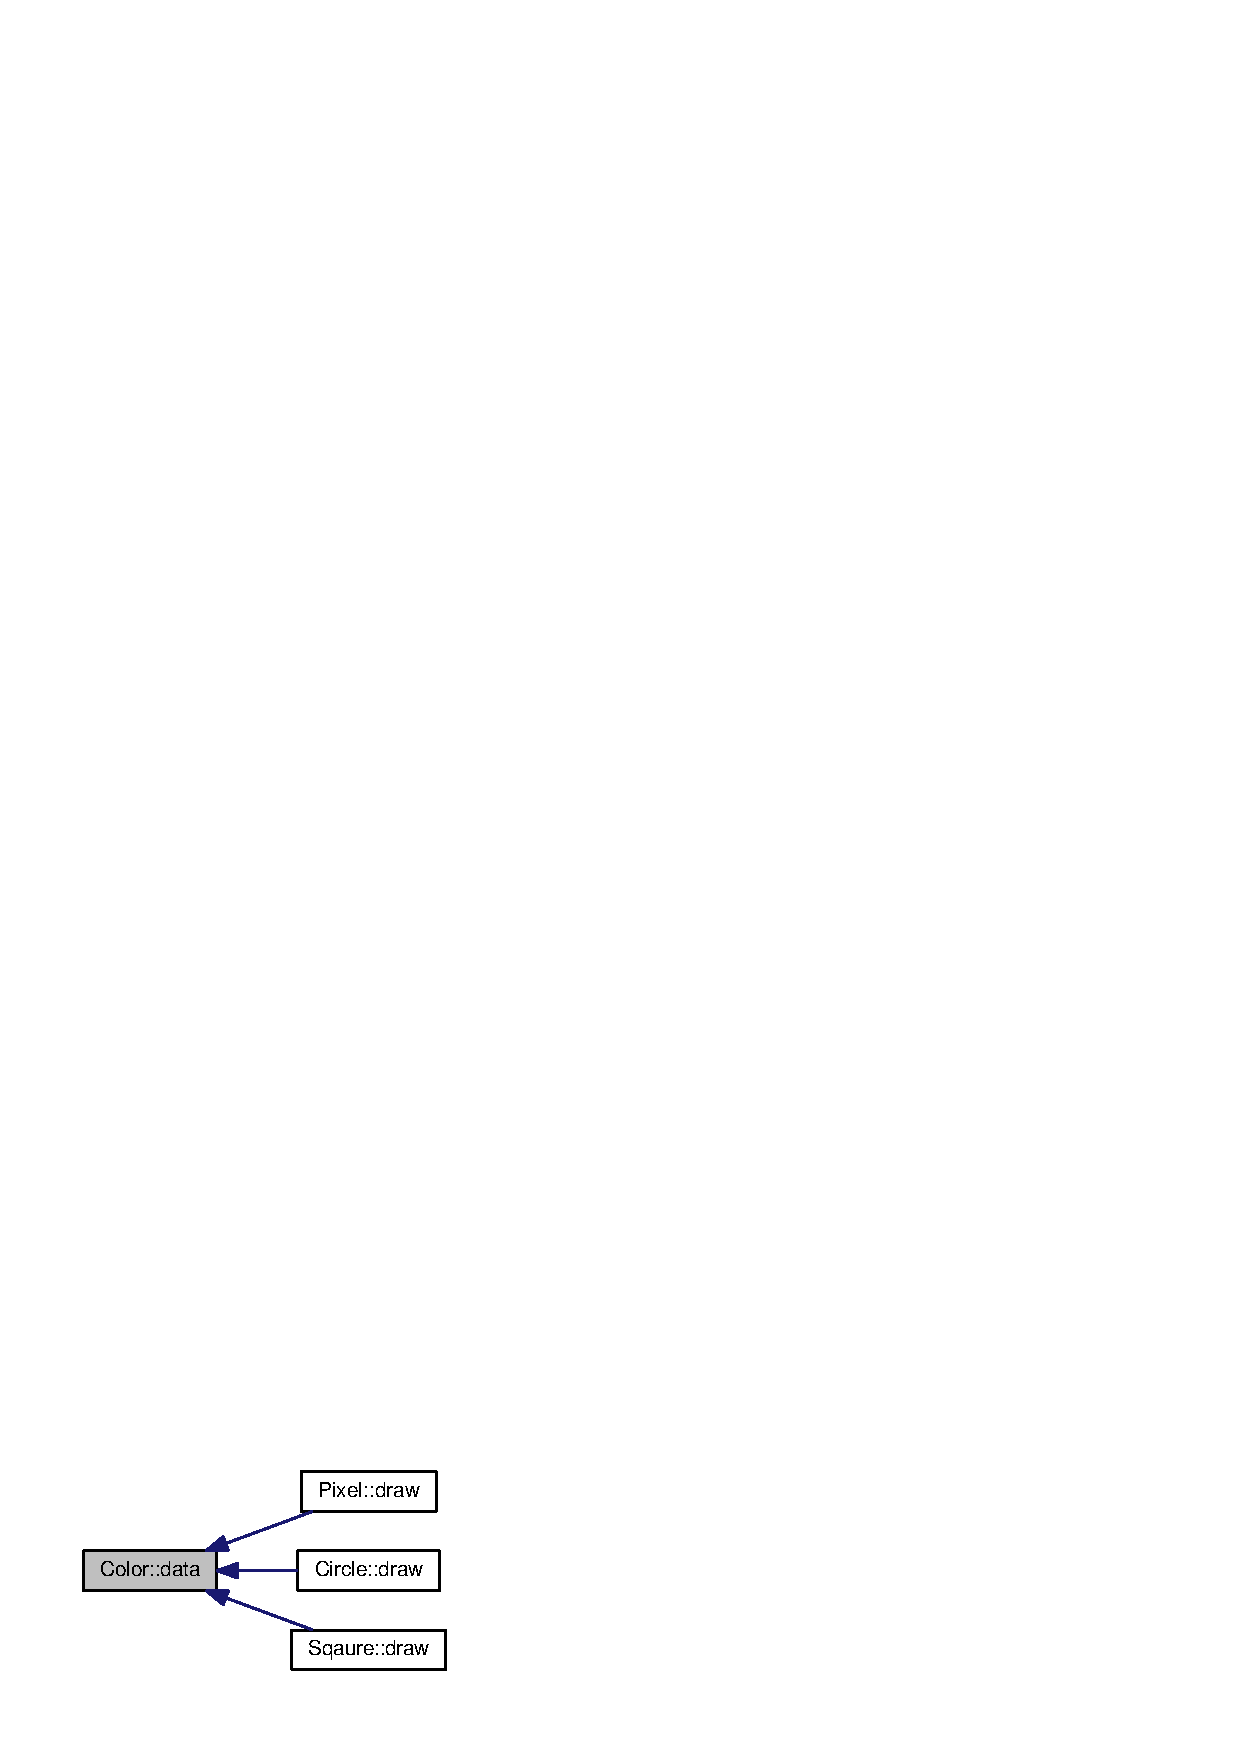
\includegraphics[width=254pt]{struct_color_a40cd03d7f9e5f481f163ddefff8e8cee_icgraph}
\end{center}
\end{figure}


\index{Color@{Color}!data@{data}}
\index{data@{data}!Color@{Color}}
\subsubsection[{\texorpdfstring{data() const }{data() const }}]{\setlength{\rightskip}{0pt plus 5cm}const float$\ast$ Color\+::data (
\begin{DoxyParamCaption}
{}
\end{DoxyParamCaption}
) const\hspace{0.3cm}{\ttfamily [inline]}}\hypertarget{struct_color_aa38a1482c148509679a046239bf9a3d9}{}\label{struct_color_aa38a1482c148509679a046239bf9a3d9}
\index{Color@{Color}!g@{g}}
\index{g@{g}!Color@{Color}}
\subsubsection[{\texorpdfstring{g()}{g()}}]{\setlength{\rightskip}{0pt plus 5cm}float\& Color\+::g (
\begin{DoxyParamCaption}
{}
\end{DoxyParamCaption}
)\hspace{0.3cm}{\ttfamily [inline]}}\hypertarget{struct_color_a4b63eac9efcfc3f626f10f43f4f13391}{}\label{struct_color_a4b63eac9efcfc3f626f10f43f4f13391}
\index{Color@{Color}!g@{g}}
\index{g@{g}!Color@{Color}}
\subsubsection[{\texorpdfstring{g() const }{g() const }}]{\setlength{\rightskip}{0pt plus 5cm}const float\& Color\+::g (
\begin{DoxyParamCaption}
{}
\end{DoxyParamCaption}
) const\hspace{0.3cm}{\ttfamily [inline]}}\hypertarget{struct_color_a47cf7afc5de2d5e3521a7fee442a9b24}{}\label{struct_color_a47cf7afc5de2d5e3521a7fee442a9b24}
\index{Color@{Color}!operator\mbox{[}$\,$\mbox{]}@{operator[]}}
\index{operator\mbox{[}$\,$\mbox{]}@{operator[]}!Color@{Color}}
\subsubsection[{\texorpdfstring{operator[](int i)}{operator[](int i)}}]{\setlength{\rightskip}{0pt plus 5cm}float\& Color\+::operator\mbox{[}$\,$\mbox{]} (
\begin{DoxyParamCaption}
\item[{int}]{i}
\end{DoxyParamCaption}
)\hspace{0.3cm}{\ttfamily [inline]}}\hypertarget{struct_color_a825baaf508fa1fc1e7a5ed2715f21d95}{}\label{struct_color_a825baaf508fa1fc1e7a5ed2715f21d95}
\index{Color@{Color}!operator\mbox{[}$\,$\mbox{]}@{operator[]}}
\index{operator\mbox{[}$\,$\mbox{]}@{operator[]}!Color@{Color}}
\subsubsection[{\texorpdfstring{operator[](int i) const }{operator[](int i) const }}]{\setlength{\rightskip}{0pt plus 5cm}const float\& Color\+::operator\mbox{[}$\,$\mbox{]} (
\begin{DoxyParamCaption}
\item[{int}]{i}
\end{DoxyParamCaption}
) const\hspace{0.3cm}{\ttfamily [inline]}}\hypertarget{struct_color_a5fa45b9e99a450800071d85b7ea1597e}{}\label{struct_color_a5fa45b9e99a450800071d85b7ea1597e}
\index{Color@{Color}!r@{r}}
\index{r@{r}!Color@{Color}}
\subsubsection[{\texorpdfstring{r()}{r()}}]{\setlength{\rightskip}{0pt plus 5cm}float\& Color\+::r (
\begin{DoxyParamCaption}
{}
\end{DoxyParamCaption}
)\hspace{0.3cm}{\ttfamily [inline]}}\hypertarget{struct_color_a9023bb1107a89197950986157c4ef9de}{}\label{struct_color_a9023bb1107a89197950986157c4ef9de}
\index{Color@{Color}!r@{r}}
\index{r@{r}!Color@{Color}}
\subsubsection[{\texorpdfstring{r() const }{r() const }}]{\setlength{\rightskip}{0pt plus 5cm}const float\& Color\+::r (
\begin{DoxyParamCaption}
{}
\end{DoxyParamCaption}
) const\hspace{0.3cm}{\ttfamily [inline]}}\hypertarget{struct_color_aa8c2969df95019d942a36793120248f6}{}\label{struct_color_aa8c2969df95019d942a36793120248f6}


The documentation for this struct was generated from the following file\+:\begin{DoxyCompactItemize}
\item 
Open\+G\+L\+Skeleton/\hyperlink{drawtools_8h}{drawtools.\+h}\end{DoxyCompactItemize}

\hypertarget{class_drawable}{}\section{Drawable Class Reference}
\label{class_drawable}\index{Drawable@{Drawable}}


{\ttfamily \#include $<$drawlist.\+h$>$}



Inheritance diagram for Drawable\+:
\nopagebreak
\begin{figure}[H]
\begin{center}
\leavevmode
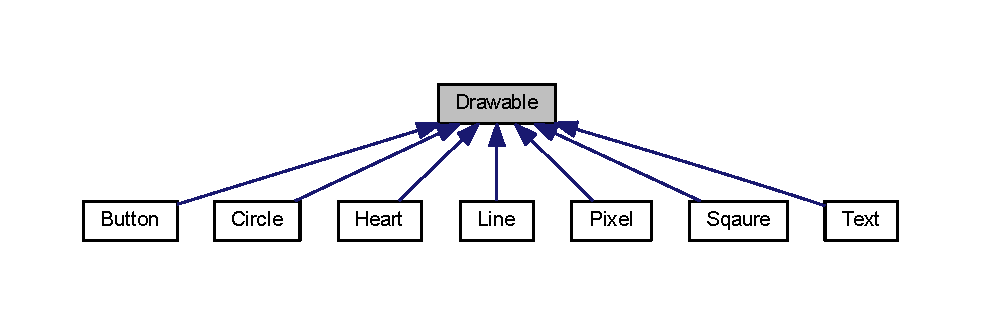
\includegraphics[width=350pt]{class_drawable__inherit__graph}
\end{center}
\end{figure}
\subsection*{Public Member Functions}
\begin{DoxyCompactItemize}
\item 
\hyperlink{class_drawable_a611d8615c65f4c7422db5f50941cd545}{Drawable} ()=default
\item 
\hyperlink{class_drawable_ac28ad19ed255d2aceee5b55b770e1377}{Drawable} (const std\+::string \&\hyperlink{class_drawable_a87794e3f62ed7128a85afee558460ae0}{name})
\item 
virtual \hyperlink{class_drawable_a489905d7db51e37ceee8fc7eaff6a762}{$\sim$\+Drawable} ()=default
\item 
virtual void \hyperlink{class_drawable_a3b1a9e1398c758f1940ffa48938c35df}{draw} () const  =0
\item 
virtual void \hyperlink{class_drawable_a7c2f20125950862e6b68109697d30076}{print} () const  =0
\item 
const std\+::string \& \hyperlink{class_drawable_a87794e3f62ed7128a85afee558460ae0}{name} () const 
\end{DoxyCompactItemize}


\subsection{Constructor \& Destructor Documentation}
\index{Drawable@{Drawable}!Drawable@{Drawable}}
\index{Drawable@{Drawable}!Drawable@{Drawable}}
\subsubsection[{\texorpdfstring{Drawable()=default}{Drawable()=default}}]{\setlength{\rightskip}{0pt plus 5cm}Drawable\+::\+Drawable (
\begin{DoxyParamCaption}
{}
\end{DoxyParamCaption}
)\hspace{0.3cm}{\ttfamily [default]}}\hypertarget{class_drawable_a611d8615c65f4c7422db5f50941cd545}{}\label{class_drawable_a611d8615c65f4c7422db5f50941cd545}
\index{Drawable@{Drawable}!Drawable@{Drawable}}
\index{Drawable@{Drawable}!Drawable@{Drawable}}
\subsubsection[{\texorpdfstring{Drawable(const std\+::string \&name)}{Drawable(const std::string &name)}}]{\setlength{\rightskip}{0pt plus 5cm}Drawable\+::\+Drawable (
\begin{DoxyParamCaption}
\item[{const std\+::string \&}]{name}
\end{DoxyParamCaption}
)}\hypertarget{class_drawable_ac28ad19ed255d2aceee5b55b770e1377}{}\label{class_drawable_ac28ad19ed255d2aceee5b55b770e1377}
\index{Drawable@{Drawable}!````~Drawable@{$\sim$\+Drawable}}
\index{````~Drawable@{$\sim$\+Drawable}!Drawable@{Drawable}}
\subsubsection[{\texorpdfstring{$\sim$\+Drawable()=default}{~Drawable()=default}}]{\setlength{\rightskip}{0pt plus 5cm}virtual Drawable\+::$\sim$\+Drawable (
\begin{DoxyParamCaption}
{}
\end{DoxyParamCaption}
)\hspace{0.3cm}{\ttfamily [virtual]}, {\ttfamily [default]}}\hypertarget{class_drawable_a489905d7db51e37ceee8fc7eaff6a762}{}\label{class_drawable_a489905d7db51e37ceee8fc7eaff6a762}


\subsection{Member Function Documentation}
\index{Drawable@{Drawable}!draw@{draw}}
\index{draw@{draw}!Drawable@{Drawable}}
\subsubsection[{\texorpdfstring{draw() const  =0}{draw() const  =0}}]{\setlength{\rightskip}{0pt plus 5cm}virtual void Drawable\+::draw (
\begin{DoxyParamCaption}
{}
\end{DoxyParamCaption}
) const\hspace{0.3cm}{\ttfamily [pure virtual]}}\hypertarget{class_drawable_a3b1a9e1398c758f1940ffa48938c35df}{}\label{class_drawable_a3b1a9e1398c758f1940ffa48938c35df}


Implemented in \hyperlink{class_button_aeb1ff67de69aef54504f36871e247edd}{Button}, \hyperlink{class_heart_a288df9fdfc652524ab2d61664bf78372}{Heart}, \hyperlink{class_text_a7216b35c6425969c0a103ec4e8ab035b}{Text}, \hyperlink{class_sqaure_add5bf042e4d2785db26c17584d3e407e}{Sqaure}, \hyperlink{class_circle_ac80d2faf29eab56f1a5c041424a07db8}{Circle}, \hyperlink{class_line_a4888aed5e5a7e51f86362eeb6ff68a6f}{Line}, and \hyperlink{class_pixel_a1b4934d22350c083260da1d5072c7a16}{Pixel}.

\index{Drawable@{Drawable}!name@{name}}
\index{name@{name}!Drawable@{Drawable}}
\subsubsection[{\texorpdfstring{name() const }{name() const }}]{\setlength{\rightskip}{0pt plus 5cm}const std\+::string \& Drawable\+::name (
\begin{DoxyParamCaption}
{}
\end{DoxyParamCaption}
) const}\hypertarget{class_drawable_a87794e3f62ed7128a85afee558460ae0}{}\label{class_drawable_a87794e3f62ed7128a85afee558460ae0}
\index{Drawable@{Drawable}!print@{print}}
\index{print@{print}!Drawable@{Drawable}}
\subsubsection[{\texorpdfstring{print() const  =0}{print() const  =0}}]{\setlength{\rightskip}{0pt plus 5cm}virtual void Drawable\+::print (
\begin{DoxyParamCaption}
{}
\end{DoxyParamCaption}
) const\hspace{0.3cm}{\ttfamily [pure virtual]}}\hypertarget{class_drawable_a7c2f20125950862e6b68109697d30076}{}\label{class_drawable_a7c2f20125950862e6b68109697d30076}


Implemented in \hyperlink{class_button_a1a416884dd2bfbf3570358200bbc0ba6}{Button}, \hyperlink{class_heart_aa097e9bf47b03cee55724db6b5f1c80d}{Heart}, \hyperlink{class_text_ac8f8d4208050ddfdeea3bb7bb4d52939}{Text}, \hyperlink{class_sqaure_a6a920c167c227af42d704d3184820140}{Sqaure}, \hyperlink{class_circle_a1410f18d9caec03103d23c162ccce1d1}{Circle}, \hyperlink{class_line_afde7d113f49b62a76836972013e1af14}{Line}, and \hyperlink{class_pixel_a221ff226e8e4485cb0ce5b9caa243808}{Pixel}.



The documentation for this class was generated from the following files\+:\begin{DoxyCompactItemize}
\item 
Open\+G\+L\+Skeleton/\hyperlink{drawlist_8h}{drawlist.\+h}\item 
Open\+G\+L\+Skeleton/\hyperlink{drawlist_8cpp}{drawlist.\+cpp}\end{DoxyCompactItemize}

\hypertarget{class_enemy}{}\section{Enemy Class Reference}
\label{class_enemy}\index{Enemy@{Enemy}}


{\ttfamily \#include $<$Enemy.\+h$>$}



Collaboration diagram for Enemy\+:
% FIG 0
\subsection*{Public Member Functions}
\begin{DoxyCompactItemize}
\item 
\hyperlink{class_enemy_a071d0a60046e25ffe08ea7be368d6693}{Enemy} (const \hyperlink{drawtools_8h_adc4a66bcb59b74164130ed47cb387ec3}{PointF} \&begin, \hyperlink{drawtools_8h_adc4a66bcb59b74164130ed47cb387ec3}{PointF} current, float speed, int health)
\item 
void \hyperlink{class_enemy_a7eb5149d39871cd4b004af55544e7764}{Health} (int i)
\item 
virtual \hyperlink{drawtools_8h_adc4a66bcb59b74164130ed47cb387ec3}{PointF} \hyperlink{class_enemy_a0ce854e74bf13c8e0d272490e29e4542}{Move} (int i, int j)
\item 
int \hyperlink{class_enemy_a1468172359f52b6f3616d3dddf5d2b0b}{Update} (\hyperlink{drawtools_8h_adc4a66bcb59b74164130ed47cb387ec3}{PointF} current)
\item 
\hyperlink{drawtools_8h_adc4a66bcb59b74164130ed47cb387ec3}{PointF} \hyperlink{class_enemy_a2fb6127ab87c9cb03eda0c1da8cefd81}{Value} ()
\end{DoxyCompactItemize}
\subsection*{Public Attributes}
\begin{DoxyCompactItemize}
\item 
\hyperlink{drawtools_8h_adc4a66bcb59b74164130ed47cb387ec3}{PointF} \hyperlink{class_enemy_a01a372cdebe6f7c5aa819aff02e3d817}{\+\_\+begin}
\item 
\hyperlink{drawtools_8h_adc4a66bcb59b74164130ed47cb387ec3}{PointF} \hyperlink{class_enemy_a2e53518ca8125c08fd204e3bf810fc8d}{\+\_\+current}
\item 
int \hyperlink{class_enemy_a410845277e89ce6c73b2df15d0621cf7}{\+\_\+health}
\item 
int \hyperlink{class_enemy_abb5f5667c06218536bf516b249d2d4cb}{\+\_\+id}
\item 
float \hyperlink{class_enemy_a5ad8a827b28dd24331a434d1993d5c01}{\+\_\+speed}
\end{DoxyCompactItemize}


\subsection{Constructor \& Destructor Documentation}
\index{Enemy@{Enemy}!Enemy@{Enemy}}
\index{Enemy@{Enemy}!Enemy@{Enemy}}
\subsubsection[{\texorpdfstring{Enemy(const Point\+F \&begin, Point\+F current, float speed, int health)}{Enemy(const PointF &begin, PointF current, float speed, int health)}}]{\setlength{\rightskip}{0pt plus 5cm}Enemy\+::\+Enemy (
\begin{DoxyParamCaption}
\item[{const {\bf PointF} \&}]{begin, }
\item[{{\bf PointF}}]{current, }
\item[{float}]{speed, }
\item[{int}]{health}
\end{DoxyParamCaption}
)}\hypertarget{class_enemy_a071d0a60046e25ffe08ea7be368d6693}{}\label{class_enemy_a071d0a60046e25ffe08ea7be368d6693}


\subsection{Member Function Documentation}
\index{Enemy@{Enemy}!Health@{Health}}
\index{Health@{Health}!Enemy@{Enemy}}
\subsubsection[{\texorpdfstring{Health(int i)}{Health(int i)}}]{\setlength{\rightskip}{0pt plus 5cm}void Enemy\+::\+Health (
\begin{DoxyParamCaption}
\item[{int}]{i}
\end{DoxyParamCaption}
)}\hypertarget{class_enemy_a7eb5149d39871cd4b004af55544e7764}{}\label{class_enemy_a7eb5149d39871cd4b004af55544e7764}
\index{Enemy@{Enemy}!Move@{Move}}
\index{Move@{Move}!Enemy@{Enemy}}
\subsubsection[{\texorpdfstring{Move(int i, int j)}{Move(int i, int j)}}]{\setlength{\rightskip}{0pt plus 5cm}{\bf PointF} Enemy\+::\+Move (
\begin{DoxyParamCaption}
\item[{int}]{i, }
\item[{int}]{j}
\end{DoxyParamCaption}
)\hspace{0.3cm}{\ttfamily [virtual]}}\hypertarget{class_enemy_a0ce854e74bf13c8e0d272490e29e4542}{}\label{class_enemy_a0ce854e74bf13c8e0d272490e29e4542}


Here is the call graph for this function\+:
% FIG 1




Here is the caller graph for this function\+:
% FIG 2


\index{Enemy@{Enemy}!Update@{Update}}
\index{Update@{Update}!Enemy@{Enemy}}
\subsubsection[{\texorpdfstring{Update(\+Point\+F current)}{Update(PointF current)}}]{\setlength{\rightskip}{0pt plus 5cm}int Enemy\+::\+Update (
\begin{DoxyParamCaption}
\item[{{\bf PointF}}]{current}
\end{DoxyParamCaption}
)}\hypertarget{class_enemy_a1468172359f52b6f3616d3dddf5d2b0b}{}\label{class_enemy_a1468172359f52b6f3616d3dddf5d2b0b}
\index{Enemy@{Enemy}!Value@{Value}}
\index{Value@{Value}!Enemy@{Enemy}}
\subsubsection[{\texorpdfstring{Value()}{Value()}}]{\setlength{\rightskip}{0pt plus 5cm}{\bf PointF} Enemy\+::\+Value (
\begin{DoxyParamCaption}
{}
\end{DoxyParamCaption}
)}\hypertarget{class_enemy_a2fb6127ab87c9cb03eda0c1da8cefd81}{}\label{class_enemy_a2fb6127ab87c9cb03eda0c1da8cefd81}


\subsection{Member Data Documentation}
\index{Enemy@{Enemy}!\+\_\+begin@{\+\_\+begin}}
\index{\+\_\+begin@{\+\_\+begin}!Enemy@{Enemy}}
\subsubsection[{\texorpdfstring{\+\_\+begin}{_begin}}]{\setlength{\rightskip}{0pt plus 5cm}{\bf PointF} Enemy\+::\+\_\+begin}\hypertarget{class_enemy_a01a372cdebe6f7c5aa819aff02e3d817}{}\label{class_enemy_a01a372cdebe6f7c5aa819aff02e3d817}
\index{Enemy@{Enemy}!\+\_\+current@{\+\_\+current}}
\index{\+\_\+current@{\+\_\+current}!Enemy@{Enemy}}
\subsubsection[{\texorpdfstring{\+\_\+current}{_current}}]{\setlength{\rightskip}{0pt plus 5cm}{\bf PointF} Enemy\+::\+\_\+current}\hypertarget{class_enemy_a2e53518ca8125c08fd204e3bf810fc8d}{}\label{class_enemy_a2e53518ca8125c08fd204e3bf810fc8d}
\index{Enemy@{Enemy}!\+\_\+health@{\+\_\+health}}
\index{\+\_\+health@{\+\_\+health}!Enemy@{Enemy}}
\subsubsection[{\texorpdfstring{\+\_\+health}{_health}}]{\setlength{\rightskip}{0pt plus 5cm}int Enemy\+::\+\_\+health}\hypertarget{class_enemy_a410845277e89ce6c73b2df15d0621cf7}{}\label{class_enemy_a410845277e89ce6c73b2df15d0621cf7}
\index{Enemy@{Enemy}!\+\_\+id@{\+\_\+id}}
\index{\+\_\+id@{\+\_\+id}!Enemy@{Enemy}}
\subsubsection[{\texorpdfstring{\+\_\+id}{_id}}]{\setlength{\rightskip}{0pt plus 5cm}int Enemy\+::\+\_\+id}\hypertarget{class_enemy_abb5f5667c06218536bf516b249d2d4cb}{}\label{class_enemy_abb5f5667c06218536bf516b249d2d4cb}
\index{Enemy@{Enemy}!\+\_\+speed@{\+\_\+speed}}
\index{\+\_\+speed@{\+\_\+speed}!Enemy@{Enemy}}
\subsubsection[{\texorpdfstring{\+\_\+speed}{_speed}}]{\setlength{\rightskip}{0pt plus 5cm}float Enemy\+::\+\_\+speed}\hypertarget{class_enemy_a5ad8a827b28dd24331a434d1993d5c01}{}\label{class_enemy_a5ad8a827b28dd24331a434d1993d5c01}


The documentation for this class was generated from the following files\+:\begin{DoxyCompactItemize}
\item 
Open\+G\+L\+Skeleton/\hyperlink{_enemy_8h}{Enemy.\+h}\item 
Open\+G\+L\+Skeleton/\hyperlink{_enemy_8cpp}{Enemy.\+cpp}\end{DoxyCompactItemize}

\hypertarget{class_fired_bullet}{}\section{Fired\+Bullet Class Reference}
\label{class_fired_bullet}\index{Fired\+Bullet@{Fired\+Bullet}}


{\ttfamily \#include $<$Fired\+Bullet.\+h$>$}



Collaboration diagram for Fired\+Bullet\+:\nopagebreak
\begin{figure}[H]
\begin{center}
\leavevmode
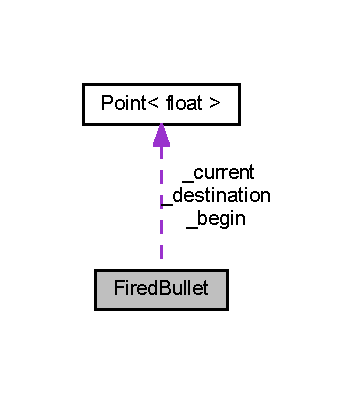
\includegraphics[width=171pt]{class_fired_bullet__coll__graph}
\end{center}
\end{figure}
\subsection*{Public Member Functions}
\begin{DoxyCompactItemize}
\item 
\hyperlink{class_fired_bullet_a529de1e268d0b6c42250b9990d5b78d0}{Fired\+Bullet} (\hyperlink{drawtools_8h_adc4a66bcb59b74164130ed47cb387ec3}{PointF} destination, \hyperlink{drawtools_8h_adc4a66bcb59b74164130ed47cb387ec3}{PointF} begin, \hyperlink{drawtools_8h_adc4a66bcb59b74164130ed47cb387ec3}{PointF} current, int speed)
\item 
\hyperlink{class_fired_bullet_a81edafb3aafe161e1757cf90d84725df}{$\sim$\+Fired\+Bullet} ()
\item 
\hyperlink{drawtools_8h_adc4a66bcb59b74164130ed47cb387ec3}{PointF} \hyperlink{class_fired_bullet_ad539d4400ec29a8d5acf32894c14c343}{Move} ()
\item 
\hyperlink{drawtools_8h_adc4a66bcb59b74164130ed47cb387ec3}{PointF} \hyperlink{class_fired_bullet_a23c23a8751529c4a6b65cb3834590c4a}{Move2} ()
\item 
void \hyperlink{class_fired_bullet_a2bd7ebc645c7db940bf3c97d57f25267}{Update} (\hyperlink{drawtools_8h_adc4a66bcb59b74164130ed47cb387ec3}{PointF} begin)
\item 
void \hyperlink{class_fired_bullet_a6517ef78bdc537d556083c093ad6ba91}{Update2} (\hyperlink{drawtools_8h_adc4a66bcb59b74164130ed47cb387ec3}{PointF} begin)
\end{DoxyCompactItemize}
\subsection*{Public Attributes}
\begin{DoxyCompactItemize}
\item 
\hyperlink{drawtools_8h_adc4a66bcb59b74164130ed47cb387ec3}{PointF} \hyperlink{class_fired_bullet_ad375a79880642a62919962703d517647}{\+\_\+begin}
\item 
\hyperlink{drawtools_8h_adc4a66bcb59b74164130ed47cb387ec3}{PointF} \hyperlink{class_fired_bullet_a288c5a49e15534f75c3ec5fde81dfa28}{\+\_\+destination}
\item 
\hyperlink{drawtools_8h_adc4a66bcb59b74164130ed47cb387ec3}{PointF} \hyperlink{class_fired_bullet_a6dd6875fc874a58132ecd2972c382889}{\+\_\+current}
\item 
int \hyperlink{class_fired_bullet_a740fdbda74e1c585cc1771d56d2a9807}{\+\_\+speed}
\item 
int \hyperlink{class_fired_bullet_aec3fb0f356070b8dfa295b771f8afb2e}{\+\_\+id}
\end{DoxyCompactItemize}


\subsection{Constructor \& Destructor Documentation}
\index{Fired\+Bullet@{Fired\+Bullet}!Fired\+Bullet@{Fired\+Bullet}}
\index{Fired\+Bullet@{Fired\+Bullet}!Fired\+Bullet@{Fired\+Bullet}}
\subsubsection[{\texorpdfstring{Fired\+Bullet(\+Point\+F destination, Point\+F begin, Point\+F current, int speed)}{FiredBullet(PointF destination, PointF begin, PointF current, int speed)}}]{\setlength{\rightskip}{0pt plus 5cm}Fired\+Bullet\+::\+Fired\+Bullet (
\begin{DoxyParamCaption}
\item[{{\bf PointF}}]{destination, }
\item[{{\bf PointF}}]{begin, }
\item[{{\bf PointF}}]{current, }
\item[{int}]{speed}
\end{DoxyParamCaption}
)}\hypertarget{class_fired_bullet_a529de1e268d0b6c42250b9990d5b78d0}{}\label{class_fired_bullet_a529de1e268d0b6c42250b9990d5b78d0}
\index{Fired\+Bullet@{Fired\+Bullet}!````~Fired\+Bullet@{$\sim$\+Fired\+Bullet}}
\index{````~Fired\+Bullet@{$\sim$\+Fired\+Bullet}!Fired\+Bullet@{Fired\+Bullet}}
\subsubsection[{\texorpdfstring{$\sim$\+Fired\+Bullet()}{~FiredBullet()}}]{\setlength{\rightskip}{0pt plus 5cm}Fired\+Bullet\+::$\sim$\+Fired\+Bullet (
\begin{DoxyParamCaption}
{}
\end{DoxyParamCaption}
)}\hypertarget{class_fired_bullet_a81edafb3aafe161e1757cf90d84725df}{}\label{class_fired_bullet_a81edafb3aafe161e1757cf90d84725df}


\subsection{Member Function Documentation}
\index{Fired\+Bullet@{Fired\+Bullet}!Move@{Move}}
\index{Move@{Move}!Fired\+Bullet@{Fired\+Bullet}}
\subsubsection[{\texorpdfstring{Move()}{Move()}}]{\setlength{\rightskip}{0pt plus 5cm}{\bf PointF} Fired\+Bullet\+::\+Move (
\begin{DoxyParamCaption}
{}
\end{DoxyParamCaption}
)}\hypertarget{class_fired_bullet_ad539d4400ec29a8d5acf32894c14c343}{}\label{class_fired_bullet_ad539d4400ec29a8d5acf32894c14c343}
\index{Fired\+Bullet@{Fired\+Bullet}!Move2@{Move2}}
\index{Move2@{Move2}!Fired\+Bullet@{Fired\+Bullet}}
\subsubsection[{\texorpdfstring{Move2()}{Move2()}}]{\setlength{\rightskip}{0pt plus 5cm}{\bf PointF} Fired\+Bullet\+::\+Move2 (
\begin{DoxyParamCaption}
{}
\end{DoxyParamCaption}
)}\hypertarget{class_fired_bullet_a23c23a8751529c4a6b65cb3834590c4a}{}\label{class_fired_bullet_a23c23a8751529c4a6b65cb3834590c4a}
\index{Fired\+Bullet@{Fired\+Bullet}!Update@{Update}}
\index{Update@{Update}!Fired\+Bullet@{Fired\+Bullet}}
\subsubsection[{\texorpdfstring{Update(\+Point\+F begin)}{Update(PointF begin)}}]{\setlength{\rightskip}{0pt plus 5cm}void Fired\+Bullet\+::\+Update (
\begin{DoxyParamCaption}
\item[{{\bf PointF}}]{begin}
\end{DoxyParamCaption}
)}\hypertarget{class_fired_bullet_a2bd7ebc645c7db940bf3c97d57f25267}{}\label{class_fired_bullet_a2bd7ebc645c7db940bf3c97d57f25267}
\index{Fired\+Bullet@{Fired\+Bullet}!Update2@{Update2}}
\index{Update2@{Update2}!Fired\+Bullet@{Fired\+Bullet}}
\subsubsection[{\texorpdfstring{Update2(\+Point\+F begin)}{Update2(PointF begin)}}]{\setlength{\rightskip}{0pt plus 5cm}void Fired\+Bullet\+::\+Update2 (
\begin{DoxyParamCaption}
\item[{{\bf PointF}}]{begin}
\end{DoxyParamCaption}
)}\hypertarget{class_fired_bullet_a6517ef78bdc537d556083c093ad6ba91}{}\label{class_fired_bullet_a6517ef78bdc537d556083c093ad6ba91}


\subsection{Member Data Documentation}
\index{Fired\+Bullet@{Fired\+Bullet}!\+\_\+begin@{\+\_\+begin}}
\index{\+\_\+begin@{\+\_\+begin}!Fired\+Bullet@{Fired\+Bullet}}
\subsubsection[{\texorpdfstring{\+\_\+begin}{_begin}}]{\setlength{\rightskip}{0pt plus 5cm}{\bf PointF} Fired\+Bullet\+::\+\_\+begin}\hypertarget{class_fired_bullet_ad375a79880642a62919962703d517647}{}\label{class_fired_bullet_ad375a79880642a62919962703d517647}
\index{Fired\+Bullet@{Fired\+Bullet}!\+\_\+current@{\+\_\+current}}
\index{\+\_\+current@{\+\_\+current}!Fired\+Bullet@{Fired\+Bullet}}
\subsubsection[{\texorpdfstring{\+\_\+current}{_current}}]{\setlength{\rightskip}{0pt plus 5cm}{\bf PointF} Fired\+Bullet\+::\+\_\+current}\hypertarget{class_fired_bullet_a6dd6875fc874a58132ecd2972c382889}{}\label{class_fired_bullet_a6dd6875fc874a58132ecd2972c382889}
\index{Fired\+Bullet@{Fired\+Bullet}!\+\_\+destination@{\+\_\+destination}}
\index{\+\_\+destination@{\+\_\+destination}!Fired\+Bullet@{Fired\+Bullet}}
\subsubsection[{\texorpdfstring{\+\_\+destination}{_destination}}]{\setlength{\rightskip}{0pt plus 5cm}{\bf PointF} Fired\+Bullet\+::\+\_\+destination}\hypertarget{class_fired_bullet_a288c5a49e15534f75c3ec5fde81dfa28}{}\label{class_fired_bullet_a288c5a49e15534f75c3ec5fde81dfa28}
\index{Fired\+Bullet@{Fired\+Bullet}!\+\_\+id@{\+\_\+id}}
\index{\+\_\+id@{\+\_\+id}!Fired\+Bullet@{Fired\+Bullet}}
\subsubsection[{\texorpdfstring{\+\_\+id}{_id}}]{\setlength{\rightskip}{0pt plus 5cm}int Fired\+Bullet\+::\+\_\+id}\hypertarget{class_fired_bullet_aec3fb0f356070b8dfa295b771f8afb2e}{}\label{class_fired_bullet_aec3fb0f356070b8dfa295b771f8afb2e}
\index{Fired\+Bullet@{Fired\+Bullet}!\+\_\+speed@{\+\_\+speed}}
\index{\+\_\+speed@{\+\_\+speed}!Fired\+Bullet@{Fired\+Bullet}}
\subsubsection[{\texorpdfstring{\+\_\+speed}{_speed}}]{\setlength{\rightskip}{0pt plus 5cm}int Fired\+Bullet\+::\+\_\+speed}\hypertarget{class_fired_bullet_a740fdbda74e1c585cc1771d56d2a9807}{}\label{class_fired_bullet_a740fdbda74e1c585cc1771d56d2a9807}


The documentation for this class was generated from the following files\+:\begin{DoxyCompactItemize}
\item 
Open\+G\+L\+Skeleton/\hyperlink{_fired_bullet_8h}{Fired\+Bullet.\+h}\item 
Open\+G\+L\+Skeleton/\hyperlink{_fired_bullet_8cpp}{Fired\+Bullet.\+cpp}\end{DoxyCompactItemize}

\section{Line Class Reference}
\label{class_line}\index{Line@{Line}}


{\ttfamily \#include $<$drawtools.\+h$>$}



Inheritance diagram for Line\+:
% FIG 0


Collaboration diagram for Line\+:
% FIG 1
\subsection*{Public Member Functions}
\begin{DoxyCompactItemize}
\item 
{\bf Line} (const {\bf PointF} \&{\bf begin}, const {\bf PointF} \&{\bf end}, const {\bf Color} \&color, float line\+Width)
\item 
const {\bf PointF} \& {\bf begin} () const 
\item 
const {\bf PointF} \& {\bf end} () const 
\item 
void {\bf draw} () const  override
\item 
void {\bf print} () const  override
\end{DoxyCompactItemize}


\subsection{Constructor \& Destructor Documentation}
\index{Line@{Line}!Line@{Line}}
\index{Line@{Line}!Line@{Line}}
\subsubsection[{Line(const Point\+F \&begin, const Point\+F \&end, const Color \&color, float line\+Width)}]{\setlength{\rightskip}{0pt plus 5cm}Line\+::\+Line (
\begin{DoxyParamCaption}
\item[{const {\bf PointF} \&}]{begin, }
\item[{const {\bf PointF} \&}]{end, }
\item[{const {\bf Color} \&}]{color, }
\item[{float}]{line\+Width}
\end{DoxyParamCaption}
)}\label{class_line_a0658a468cca251fce62dc16249cdf763}


Here is the call graph for this function\+:
% FIG 2




\subsection{Member Function Documentation}
\index{Line@{Line}!begin@{begin}}
\index{begin@{begin}!Line@{Line}}
\subsubsection[{begin() const }]{\setlength{\rightskip}{0pt plus 5cm}const {\bf PointF} \& Line\+::begin (
\begin{DoxyParamCaption}
{}
\end{DoxyParamCaption}
) const}\label{class_line_a9e91a70ec8ece5196f0209f4a0432e25}
\index{Line@{Line}!draw@{draw}}
\index{draw@{draw}!Line@{Line}}
\subsubsection[{draw() const  override}]{\setlength{\rightskip}{0pt plus 5cm}void Line\+::draw (
\begin{DoxyParamCaption}
{}
\end{DoxyParamCaption}
) const\hspace{0.3cm}{\ttfamily [override]}, {\ttfamily [virtual]}}\label{class_line_a4888aed5e5a7e51f86362eeb6ff68a6f}


Implements {\bf Drawable} \doxyref{}{p.}{class_drawable_a3b1a9e1398c758f1940ffa48938c35df}.



Here is the call graph for this function\+:
% FIG 3


\index{Line@{Line}!end@{end}}
\index{end@{end}!Line@{Line}}
\subsubsection[{end() const }]{\setlength{\rightskip}{0pt plus 5cm}const {\bf PointF} \& Line\+::end (
\begin{DoxyParamCaption}
{}
\end{DoxyParamCaption}
) const}\label{class_line_a22c8bc4b1bf059fab1741b3fa7102ad0}


Here is the caller graph for this function\+:
% FIG 4


\index{Line@{Line}!print@{print}}
\index{print@{print}!Line@{Line}}
\subsubsection[{print() const  override}]{\setlength{\rightskip}{0pt plus 5cm}void Line\+::print (
\begin{DoxyParamCaption}
{}
\end{DoxyParamCaption}
) const\hspace{0.3cm}{\ttfamily [override]}, {\ttfamily [virtual]}}\label{class_line_afde7d113f49b62a76836972013e1af14}


Implements {\bf Drawable} \doxyref{}{p.}{class_drawable_a7c2f20125950862e6b68109697d30076}.



The documentation for this class was generated from the following files\+:\begin{DoxyCompactItemize}
\item 
Open\+G\+L\+Skeleton/{\bf drawtools.\+h}\item 
Open\+G\+L\+Skeleton/{\bf drawtools.\+cpp}\end{DoxyCompactItemize}

\hypertarget{class_pixel}{}\section{Pixel Class Reference}
\label{class_pixel}\index{Pixel@{Pixel}}


{\ttfamily \#include $<$drawtools.\+h$>$}



Inheritance diagram for Pixel\+:
% FIG 0


Collaboration diagram for Pixel\+:
% FIG 1
\subsection*{Public Member Functions}
\begin{DoxyCompactItemize}
\item 
\hyperlink{class_pixel_a923b96aa409817e4e8bd144643bb6ffc}{Pixel} (const \hyperlink{drawtools_8h_adc4a66bcb59b74164130ed47cb387ec3}{PointF} \&position, const \hyperlink{struct_color}{Color} \&color)
\item 
void \hyperlink{class_pixel_a1b4934d22350c083260da1d5072c7a16}{draw} () const  override
\item 
void \hyperlink{class_pixel_a221ff226e8e4485cb0ce5b9caa243808}{print} () const  override
\end{DoxyCompactItemize}


\subsection{Constructor \& Destructor Documentation}
\index{Pixel@{Pixel}!Pixel@{Pixel}}
\index{Pixel@{Pixel}!Pixel@{Pixel}}
\subsubsection[{\texorpdfstring{Pixel(const Point\+F \&position, const Color \&color)}{Pixel(const PointF &position, const Color &color)}}]{\setlength{\rightskip}{0pt plus 5cm}Pixel\+::\+Pixel (
\begin{DoxyParamCaption}
\item[{const {\bf PointF} \&}]{position, }
\item[{const {\bf Color} \&}]{color}
\end{DoxyParamCaption}
)}\hypertarget{class_pixel_a923b96aa409817e4e8bd144643bb6ffc}{}\label{class_pixel_a923b96aa409817e4e8bd144643bb6ffc}


\subsection{Member Function Documentation}
\index{Pixel@{Pixel}!draw@{draw}}
\index{draw@{draw}!Pixel@{Pixel}}
\subsubsection[{\texorpdfstring{draw() const  override}{draw() const  override}}]{\setlength{\rightskip}{0pt plus 5cm}void Pixel\+::draw (
\begin{DoxyParamCaption}
{}
\end{DoxyParamCaption}
) const\hspace{0.3cm}{\ttfamily [override]}, {\ttfamily [virtual]}}\hypertarget{class_pixel_a1b4934d22350c083260da1d5072c7a16}{}\label{class_pixel_a1b4934d22350c083260da1d5072c7a16}


Implements \hyperlink{class_drawable_a3b1a9e1398c758f1940ffa48938c35df}{Drawable}.



Here is the call graph for this function\+:
% FIG 2


\index{Pixel@{Pixel}!print@{print}}
\index{print@{print}!Pixel@{Pixel}}
\subsubsection[{\texorpdfstring{print() const  override}{print() const  override}}]{\setlength{\rightskip}{0pt plus 5cm}void Pixel\+::print (
\begin{DoxyParamCaption}
{}
\end{DoxyParamCaption}
) const\hspace{0.3cm}{\ttfamily [override]}, {\ttfamily [virtual]}}\hypertarget{class_pixel_a221ff226e8e4485cb0ce5b9caa243808}{}\label{class_pixel_a221ff226e8e4485cb0ce5b9caa243808}


Implements \hyperlink{class_drawable_a7c2f20125950862e6b68109697d30076}{Drawable}.



The documentation for this class was generated from the following files\+:\begin{DoxyCompactItemize}
\item 
Open\+G\+L\+Skeleton/\hyperlink{drawtools_8h}{drawtools.\+h}\item 
Open\+G\+L\+Skeleton/\hyperlink{drawtools_8cpp}{drawtools.\+cpp}\end{DoxyCompactItemize}

\hypertarget{class_point}{}\section{Point$<$ T $>$ Class Template Reference}
\label{class_point}\index{Point$<$ T $>$@{Point$<$ T $>$}}


{\ttfamily \#include $<$drawtools.\+h$>$}

\subsection*{Public Member Functions}
\begin{DoxyCompactItemize}
\item 
\hyperlink{class_point_ae6a75fcca567819ab05482257ce36bdc}{Point} ()=default
\item 
\hyperlink{class_point_a04dfeba9060ba82f2012fd91e51b1c0e}{Point} (const T \&\hyperlink{class_point_a97a274fff44375b5d60e209f26d7382f}{x}, const T \&\hyperlink{class_point_a71672fd35753d43129ff157127dba575}{y})
\item 
T \& \hyperlink{class_point_a97a274fff44375b5d60e209f26d7382f}{x} ()
\item 
const T \& \hyperlink{class_point_ab2318285f4b0003ae1b5eac16365da89}{x} () const 
\item 
T \& \hyperlink{class_point_a71672fd35753d43129ff157127dba575}{y} ()
\item 
const T \& \hyperlink{class_point_a3b51ef3be91aa516ec98a8d14b6bb68f}{y} () const 
\item 
T \& \hyperlink{class_point_ad678b61ba9ebd74c4a7ce6d19b37d52b}{operator\mbox{[}$\,$\mbox{]}} (int i)
\item 
const T \& \hyperlink{class_point_a793b651c93b7ec0b38d147c0fe03d0cd}{operator\mbox{[}$\,$\mbox{]}} (int i) const 
\item 
T $\ast$ \hyperlink{class_point_ad8039edae63c5cbefefc6d671ba3197b}{data} ()
\item 
const T $\ast$ \hyperlink{class_point_abff7e82df3f1517cb32aae8c05f8f176}{data} () const 
\end{DoxyCompactItemize}


\subsection{Constructor \& Destructor Documentation}
\index{Point@{Point}!Point@{Point}}
\index{Point@{Point}!Point@{Point}}
\subsubsection[{\texorpdfstring{Point()=default}{Point()=default}}]{\setlength{\rightskip}{0pt plus 5cm}template$<$typename T$>$ {\bf Point}$<$ T $>$\+::{\bf Point} (
\begin{DoxyParamCaption}
{}
\end{DoxyParamCaption}
)\hspace{0.3cm}{\ttfamily [default]}}\hypertarget{class_point_ae6a75fcca567819ab05482257ce36bdc}{}\label{class_point_ae6a75fcca567819ab05482257ce36bdc}
\index{Point@{Point}!Point@{Point}}
\index{Point@{Point}!Point@{Point}}
\subsubsection[{\texorpdfstring{Point(const T \&x, const T \&y)}{Point(const T &x, const T &y)}}]{\setlength{\rightskip}{0pt plus 5cm}template$<$typename T$>$ {\bf Point}$<$ T $>$\+::{\bf Point} (
\begin{DoxyParamCaption}
\item[{const T \&}]{x, }
\item[{const T \&}]{y}
\end{DoxyParamCaption}
)\hspace{0.3cm}{\ttfamily [inline]}}\hypertarget{class_point_a04dfeba9060ba82f2012fd91e51b1c0e}{}\label{class_point_a04dfeba9060ba82f2012fd91e51b1c0e}


\subsection{Member Function Documentation}
\index{Point@{Point}!data@{data}}
\index{data@{data}!Point@{Point}}
\subsubsection[{\texorpdfstring{data()}{data()}}]{\setlength{\rightskip}{0pt plus 5cm}template$<$typename T$>$ T$\ast$ {\bf Point}$<$ T $>$\+::data (
\begin{DoxyParamCaption}
{}
\end{DoxyParamCaption}
)\hspace{0.3cm}{\ttfamily [inline]}}\hypertarget{class_point_ad8039edae63c5cbefefc6d671ba3197b}{}\label{class_point_ad8039edae63c5cbefefc6d671ba3197b}


Here is the caller graph for this function\+:
% FIG 0


\index{Point@{Point}!data@{data}}
\index{data@{data}!Point@{Point}}
\subsubsection[{\texorpdfstring{data() const }{data() const }}]{\setlength{\rightskip}{0pt plus 5cm}template$<$typename T$>$ const T$\ast$ {\bf Point}$<$ T $>$\+::data (
\begin{DoxyParamCaption}
{}
\end{DoxyParamCaption}
) const\hspace{0.3cm}{\ttfamily [inline]}}\hypertarget{class_point_abff7e82df3f1517cb32aae8c05f8f176}{}\label{class_point_abff7e82df3f1517cb32aae8c05f8f176}
\index{Point@{Point}!operator\mbox{[}$\,$\mbox{]}@{operator[]}}
\index{operator\mbox{[}$\,$\mbox{]}@{operator[]}!Point@{Point}}
\subsubsection[{\texorpdfstring{operator[](int i)}{operator[](int i)}}]{\setlength{\rightskip}{0pt plus 5cm}template$<$typename T$>$ T\& {\bf Point}$<$ T $>$\+::operator\mbox{[}$\,$\mbox{]} (
\begin{DoxyParamCaption}
\item[{int}]{i}
\end{DoxyParamCaption}
)\hspace{0.3cm}{\ttfamily [inline]}}\hypertarget{class_point_ad678b61ba9ebd74c4a7ce6d19b37d52b}{}\label{class_point_ad678b61ba9ebd74c4a7ce6d19b37d52b}
\index{Point@{Point}!operator\mbox{[}$\,$\mbox{]}@{operator[]}}
\index{operator\mbox{[}$\,$\mbox{]}@{operator[]}!Point@{Point}}
\subsubsection[{\texorpdfstring{operator[](int i) const }{operator[](int i) const }}]{\setlength{\rightskip}{0pt plus 5cm}template$<$typename T$>$ const T\& {\bf Point}$<$ T $>$\+::operator\mbox{[}$\,$\mbox{]} (
\begin{DoxyParamCaption}
\item[{int}]{i}
\end{DoxyParamCaption}
) const\hspace{0.3cm}{\ttfamily [inline]}}\hypertarget{class_point_a793b651c93b7ec0b38d147c0fe03d0cd}{}\label{class_point_a793b651c93b7ec0b38d147c0fe03d0cd}
\index{Point@{Point}!x@{x}}
\index{x@{x}!Point@{Point}}
\subsubsection[{\texorpdfstring{x()}{x()}}]{\setlength{\rightskip}{0pt plus 5cm}template$<$typename T$>$ T\& {\bf Point}$<$ T $>$\+::x (
\begin{DoxyParamCaption}
{}
\end{DoxyParamCaption}
)\hspace{0.3cm}{\ttfamily [inline]}}\hypertarget{class_point_a97a274fff44375b5d60e209f26d7382f}{}\label{class_point_a97a274fff44375b5d60e209f26d7382f}


Here is the caller graph for this function\+:
% FIG 1


\index{Point@{Point}!x@{x}}
\index{x@{x}!Point@{Point}}
\subsubsection[{\texorpdfstring{x() const }{x() const }}]{\setlength{\rightskip}{0pt plus 5cm}template$<$typename T$>$ const T\& {\bf Point}$<$ T $>$\+::x (
\begin{DoxyParamCaption}
{}
\end{DoxyParamCaption}
) const\hspace{0.3cm}{\ttfamily [inline]}}\hypertarget{class_point_ab2318285f4b0003ae1b5eac16365da89}{}\label{class_point_ab2318285f4b0003ae1b5eac16365da89}
\index{Point@{Point}!y@{y}}
\index{y@{y}!Point@{Point}}
\subsubsection[{\texorpdfstring{y()}{y()}}]{\setlength{\rightskip}{0pt plus 5cm}template$<$typename T$>$ T\& {\bf Point}$<$ T $>$\+::y (
\begin{DoxyParamCaption}
{}
\end{DoxyParamCaption}
)\hspace{0.3cm}{\ttfamily [inline]}}\hypertarget{class_point_a71672fd35753d43129ff157127dba575}{}\label{class_point_a71672fd35753d43129ff157127dba575}


Here is the caller graph for this function\+:
% FIG 2


\index{Point@{Point}!y@{y}}
\index{y@{y}!Point@{Point}}
\subsubsection[{\texorpdfstring{y() const }{y() const }}]{\setlength{\rightskip}{0pt plus 5cm}template$<$typename T$>$ const T\& {\bf Point}$<$ T $>$\+::y (
\begin{DoxyParamCaption}
{}
\end{DoxyParamCaption}
) const\hspace{0.3cm}{\ttfamily [inline]}}\hypertarget{class_point_a3b51ef3be91aa516ec98a8d14b6bb68f}{}\label{class_point_a3b51ef3be91aa516ec98a8d14b6bb68f}


The documentation for this class was generated from the following file\+:\begin{DoxyCompactItemize}
\item 
Open\+G\+L\+Skeleton/\hyperlink{drawtools_8h}{drawtools.\+h}\end{DoxyCompactItemize}

\hypertarget{class_sqaure}{}\section{Sqaure Class Reference}
\label{class_sqaure}\index{Sqaure@{Sqaure}}


{\ttfamily \#include $<$drawtools.\+h$>$}



Inheritance diagram for Sqaure\+:\nopagebreak
\begin{figure}[H]
\begin{center}
\leavevmode
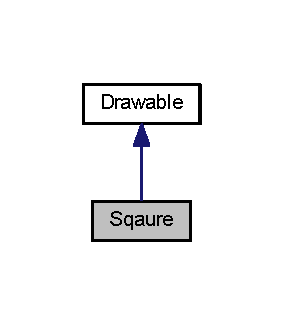
\includegraphics[width=136pt]{class_sqaure__inherit__graph}
\end{center}
\end{figure}


Collaboration diagram for Sqaure\+:\nopagebreak
\begin{figure}[H]
\begin{center}
\leavevmode
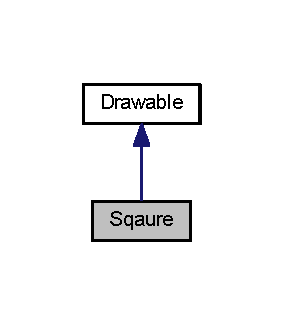
\includegraphics[width=136pt]{class_sqaure__coll__graph}
\end{center}
\end{figure}
\subsection*{Public Member Functions}
\begin{DoxyCompactItemize}
\item 
\hyperlink{class_sqaure_a64bbc7316e2c8b7e5c9096415b252206}{Sqaure} (const \hyperlink{drawtools_8h_adc4a66bcb59b74164130ed47cb387ec3}{PointF} \&begin, const \hyperlink{drawtools_8h_adc4a66bcb59b74164130ed47cb387ec3}{PointF} \&end, const \hyperlink{drawtools_8h_adc4a66bcb59b74164130ed47cb387ec3}{PointF} \&begin2, const \hyperlink{drawtools_8h_adc4a66bcb59b74164130ed47cb387ec3}{PointF} \&end2, const \hyperlink{struct_color}{Color} \&color)
\item 
void \hyperlink{class_sqaure_add5bf042e4d2785db26c17584d3e407e}{draw} () const  override
\item 
void \hyperlink{class_sqaure_a6a920c167c227af42d704d3184820140}{print} () const  override
\end{DoxyCompactItemize}


\subsection{Constructor \& Destructor Documentation}
\index{Sqaure@{Sqaure}!Sqaure@{Sqaure}}
\index{Sqaure@{Sqaure}!Sqaure@{Sqaure}}
\subsubsection[{\texorpdfstring{Sqaure(const Point\+F \&begin, const Point\+F \&end, const Point\+F \&begin2, const Point\+F \&end2, const Color \&color)}{Sqaure(const PointF &begin, const PointF &end, const PointF &begin2, const PointF &end2, const Color &color)}}]{\setlength{\rightskip}{0pt plus 5cm}Sqaure\+::\+Sqaure (
\begin{DoxyParamCaption}
\item[{const {\bf PointF} \&}]{begin, }
\item[{const {\bf PointF} \&}]{end, }
\item[{const {\bf PointF} \&}]{begin2, }
\item[{const {\bf PointF} \&}]{end2, }
\item[{const {\bf Color} \&}]{color}
\end{DoxyParamCaption}
)}\hypertarget{class_sqaure_a64bbc7316e2c8b7e5c9096415b252206}{}\label{class_sqaure_a64bbc7316e2c8b7e5c9096415b252206}


\subsection{Member Function Documentation}
\index{Sqaure@{Sqaure}!draw@{draw}}
\index{draw@{draw}!Sqaure@{Sqaure}}
\subsubsection[{\texorpdfstring{draw() const  override}{draw() const  override}}]{\setlength{\rightskip}{0pt plus 5cm}void Sqaure\+::draw (
\begin{DoxyParamCaption}
{}
\end{DoxyParamCaption}
) const\hspace{0.3cm}{\ttfamily [override]}, {\ttfamily [virtual]}}\hypertarget{class_sqaure_add5bf042e4d2785db26c17584d3e407e}{}\label{class_sqaure_add5bf042e4d2785db26c17584d3e407e}


Implements \hyperlink{class_drawable_a3b1a9e1398c758f1940ffa48938c35df}{Drawable}.



Here is the call graph for this function\+:\nopagebreak
\begin{figure}[H]
\begin{center}
\leavevmode
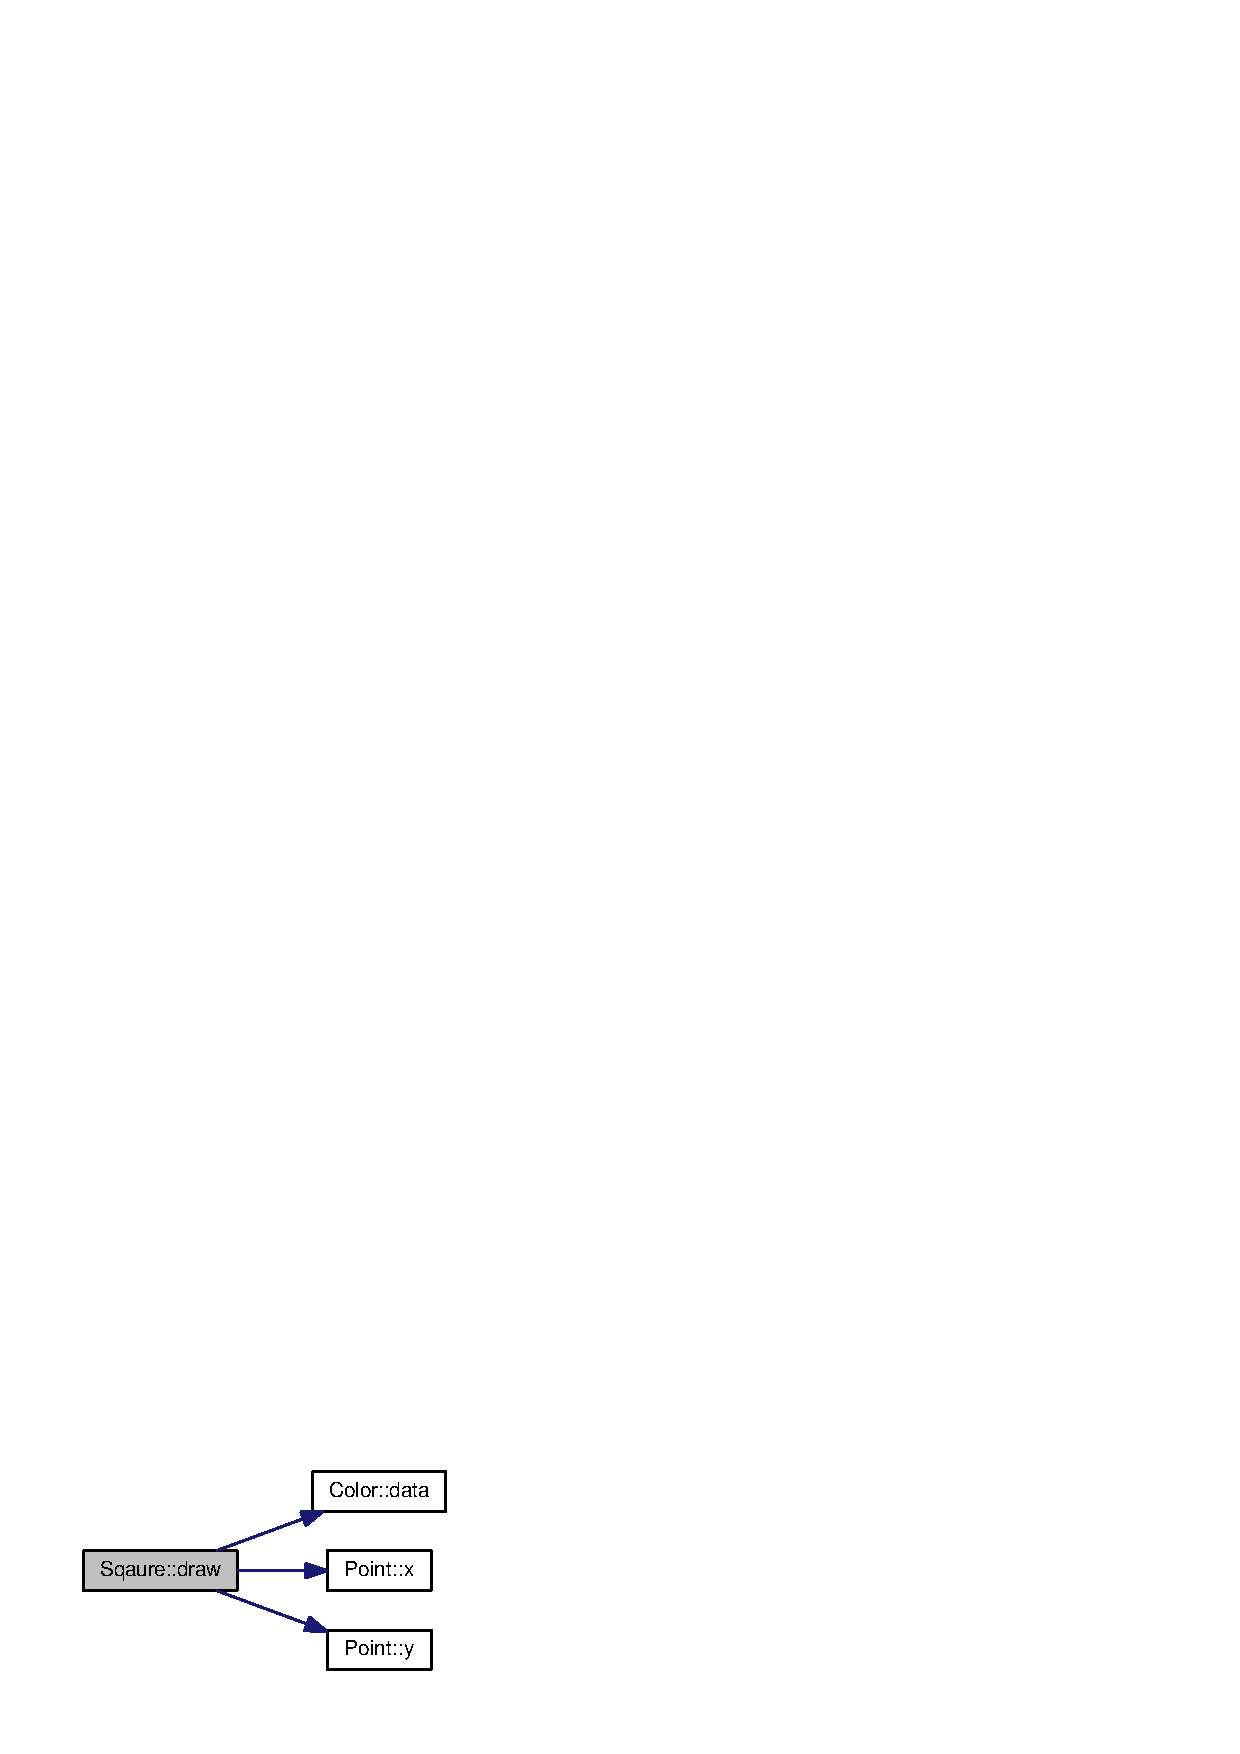
\includegraphics[width=254pt]{class_sqaure_add5bf042e4d2785db26c17584d3e407e_cgraph}
\end{center}
\end{figure}


\index{Sqaure@{Sqaure}!print@{print}}
\index{print@{print}!Sqaure@{Sqaure}}
\subsubsection[{\texorpdfstring{print() const  override}{print() const  override}}]{\setlength{\rightskip}{0pt plus 5cm}void Sqaure\+::print (
\begin{DoxyParamCaption}
{}
\end{DoxyParamCaption}
) const\hspace{0.3cm}{\ttfamily [override]}, {\ttfamily [virtual]}}\hypertarget{class_sqaure_a6a920c167c227af42d704d3184820140}{}\label{class_sqaure_a6a920c167c227af42d704d3184820140}


Implements \hyperlink{class_drawable_a7c2f20125950862e6b68109697d30076}{Drawable}.



The documentation for this class was generated from the following files\+:\begin{DoxyCompactItemize}
\item 
Open\+G\+L\+Skeleton/\hyperlink{drawtools_8h}{drawtools.\+h}\item 
Open\+G\+L\+Skeleton/\hyperlink{drawtools_8cpp}{drawtools.\+cpp}\end{DoxyCompactItemize}

\hypertarget{class_text}{}\section{Text Class Reference}
\label{class_text}\index{Text@{Text}}


{\ttfamily \#include $<$drawtools.\+h$>$}



Inheritance diagram for Text\+:
% FIG 0


Collaboration diagram for Text\+:
% FIG 1
\subsection*{Public Member Functions}
\begin{DoxyCompactItemize}
\item 
\hyperlink{class_text_a6601c5ff47564843254ee8b1a5588368}{Text} (const std\+::string \&str)
\item 
void \hyperlink{class_text_a7216b35c6425969c0a103ec4e8ab035b}{draw} () const  override
\item 
void \hyperlink{class_text_ac8f8d4208050ddfdeea3bb7bb4d52939}{print} () const  override
\end{DoxyCompactItemize}


\subsection{Constructor \& Destructor Documentation}
\index{Text@{Text}!Text@{Text}}
\index{Text@{Text}!Text@{Text}}
\subsubsection[{\texorpdfstring{Text(const std\+::string \&str)}{Text(const std::string &str)}}]{\setlength{\rightskip}{0pt plus 5cm}Text\+::\+Text (
\begin{DoxyParamCaption}
\item[{const std\+::string \&}]{str}
\end{DoxyParamCaption}
)}\hypertarget{class_text_a6601c5ff47564843254ee8b1a5588368}{}\label{class_text_a6601c5ff47564843254ee8b1a5588368}


\subsection{Member Function Documentation}
\index{Text@{Text}!draw@{draw}}
\index{draw@{draw}!Text@{Text}}
\subsubsection[{\texorpdfstring{draw() const  override}{draw() const  override}}]{\setlength{\rightskip}{0pt plus 5cm}void Text\+::draw (
\begin{DoxyParamCaption}
{}
\end{DoxyParamCaption}
) const\hspace{0.3cm}{\ttfamily [override]}, {\ttfamily [virtual]}}\hypertarget{class_text_a7216b35c6425969c0a103ec4e8ab035b}{}\label{class_text_a7216b35c6425969c0a103ec4e8ab035b}


Implements \hyperlink{class_drawable_a3b1a9e1398c758f1940ffa48938c35df}{Drawable}.

\index{Text@{Text}!print@{print}}
\index{print@{print}!Text@{Text}}
\subsubsection[{\texorpdfstring{print() const  override}{print() const  override}}]{\setlength{\rightskip}{0pt plus 5cm}void Text\+::print (
\begin{DoxyParamCaption}
{}
\end{DoxyParamCaption}
) const\hspace{0.3cm}{\ttfamily [override]}, {\ttfamily [virtual]}}\hypertarget{class_text_ac8f8d4208050ddfdeea3bb7bb4d52939}{}\label{class_text_ac8f8d4208050ddfdeea3bb7bb4d52939}


Implements \hyperlink{class_drawable_a7c2f20125950862e6b68109697d30076}{Drawable}.



The documentation for this class was generated from the following files\+:\begin{DoxyCompactItemize}
\item 
Open\+G\+L\+Skeleton/\hyperlink{drawtools_8h}{drawtools.\+h}\item 
Open\+G\+L\+Skeleton/\hyperlink{drawtools_8cpp}{drawtools.\+cpp}\end{DoxyCompactItemize}

\hypertarget{class_turret}{}\section{Turret Class Reference}
\label{class_turret}\index{Turret@{Turret}}


{\ttfamily \#include $<$Turret.\+h$>$}



Collaboration diagram for Turret\+:
% FIG 0
\subsection*{Public Member Functions}
\begin{DoxyCompactItemize}
\item 
\hyperlink{class_turret_a7c56fc2fe7272313a06fb69262f9f2e4}{Turret} (\hyperlink{drawtools_8h_adc4a66bcb59b74164130ed47cb387ec3}{PointF} position, \hyperlink{struct_color}{Color} color, int range, int health, int upgrade, int type)
\item 
int \hyperlink{class_turret_a8d3b80c4fd7534448f5e7e7ce6618062}{Aim} (int i)
\item 
\hyperlink{drawtools_8h_adc4a66bcb59b74164130ed47cb387ec3}{PointF} \hyperlink{class_turret_a86f457d14098684ab3954864b07dc560}{Position} ()
\end{DoxyCompactItemize}
\subsection*{Public Attributes}
\begin{DoxyCompactItemize}
\item 
\hyperlink{drawtools_8h_adc4a66bcb59b74164130ed47cb387ec3}{PointF} \hyperlink{class_turret_a0ef0ca5baa391a6874f97b6b3e440432}{\+\_\+position}
\item 
int \hyperlink{class_turret_a9af84b28b71291fd780c2959d331532d}{\+\_\+upgrade}
\item 
int \hyperlink{class_turret_a53bde4ee8aab3c1e2733445bfe26fb22}{\+\_\+type}
\item 
int \hyperlink{class_turret_ae0343faa95df71e2a8bf7269e617fc72}{\+\_\+range}
\item 
int \hyperlink{class_turret_ab2bf5de8417b19dd7d78f29ce041a16a}{\+\_\+health}
\item 
int \hyperlink{class_turret_a5c5b20c2a2e56f4ced002b7d79be0b25}{\+\_\+bullet\+Speed}
\item 
int \hyperlink{class_turret_a359ea4b0d1eb06880d0971dbc1c77c60}{\+\_\+aiming} = 0
\end{DoxyCompactItemize}


\subsection{Constructor \& Destructor Documentation}
\index{Turret@{Turret}!Turret@{Turret}}
\index{Turret@{Turret}!Turret@{Turret}}
\subsubsection[{\texorpdfstring{Turret(\+Point\+F position, Color color, int range, int health, int upgrade, int type)}{Turret(PointF position, Color color, int range, int health, int upgrade, int type)}}]{\setlength{\rightskip}{0pt plus 5cm}Turret\+::\+Turret (
\begin{DoxyParamCaption}
\item[{{\bf PointF}}]{position, }
\item[{{\bf Color}}]{color, }
\item[{int}]{range, }
\item[{int}]{health, }
\item[{int}]{upgrade, }
\item[{int}]{type}
\end{DoxyParamCaption}
)}\hypertarget{class_turret_a7c56fc2fe7272313a06fb69262f9f2e4}{}\label{class_turret_a7c56fc2fe7272313a06fb69262f9f2e4}


\subsection{Member Function Documentation}
\index{Turret@{Turret}!Aim@{Aim}}
\index{Aim@{Aim}!Turret@{Turret}}
\subsubsection[{\texorpdfstring{Aim(int i)}{Aim(int i)}}]{\setlength{\rightskip}{0pt plus 5cm}int Turret\+::\+Aim (
\begin{DoxyParamCaption}
\item[{int}]{i}
\end{DoxyParamCaption}
)}\hypertarget{class_turret_a8d3b80c4fd7534448f5e7e7ce6618062}{}\label{class_turret_a8d3b80c4fd7534448f5e7e7ce6618062}
\index{Turret@{Turret}!Position@{Position}}
\index{Position@{Position}!Turret@{Turret}}
\subsubsection[{\texorpdfstring{Position()}{Position()}}]{\setlength{\rightskip}{0pt plus 5cm}{\bf PointF} Turret\+::\+Position (
\begin{DoxyParamCaption}
{}
\end{DoxyParamCaption}
)}\hypertarget{class_turret_a86f457d14098684ab3954864b07dc560}{}\label{class_turret_a86f457d14098684ab3954864b07dc560}


\subsection{Member Data Documentation}
\index{Turret@{Turret}!\+\_\+aiming@{\+\_\+aiming}}
\index{\+\_\+aiming@{\+\_\+aiming}!Turret@{Turret}}
\subsubsection[{\texorpdfstring{\+\_\+aiming}{_aiming}}]{\setlength{\rightskip}{0pt plus 5cm}int Turret\+::\+\_\+aiming = 0}\hypertarget{class_turret_a359ea4b0d1eb06880d0971dbc1c77c60}{}\label{class_turret_a359ea4b0d1eb06880d0971dbc1c77c60}
\index{Turret@{Turret}!\+\_\+bullet\+Speed@{\+\_\+bullet\+Speed}}
\index{\+\_\+bullet\+Speed@{\+\_\+bullet\+Speed}!Turret@{Turret}}
\subsubsection[{\texorpdfstring{\+\_\+bullet\+Speed}{_bulletSpeed}}]{\setlength{\rightskip}{0pt plus 5cm}int Turret\+::\+\_\+bullet\+Speed}\hypertarget{class_turret_a5c5b20c2a2e56f4ced002b7d79be0b25}{}\label{class_turret_a5c5b20c2a2e56f4ced002b7d79be0b25}
\index{Turret@{Turret}!\+\_\+health@{\+\_\+health}}
\index{\+\_\+health@{\+\_\+health}!Turret@{Turret}}
\subsubsection[{\texorpdfstring{\+\_\+health}{_health}}]{\setlength{\rightskip}{0pt plus 5cm}int Turret\+::\+\_\+health}\hypertarget{class_turret_ab2bf5de8417b19dd7d78f29ce041a16a}{}\label{class_turret_ab2bf5de8417b19dd7d78f29ce041a16a}
\index{Turret@{Turret}!\+\_\+position@{\+\_\+position}}
\index{\+\_\+position@{\+\_\+position}!Turret@{Turret}}
\subsubsection[{\texorpdfstring{\+\_\+position}{_position}}]{\setlength{\rightskip}{0pt plus 5cm}{\bf PointF} Turret\+::\+\_\+position}\hypertarget{class_turret_a0ef0ca5baa391a6874f97b6b3e440432}{}\label{class_turret_a0ef0ca5baa391a6874f97b6b3e440432}
\index{Turret@{Turret}!\+\_\+range@{\+\_\+range}}
\index{\+\_\+range@{\+\_\+range}!Turret@{Turret}}
\subsubsection[{\texorpdfstring{\+\_\+range}{_range}}]{\setlength{\rightskip}{0pt plus 5cm}int Turret\+::\+\_\+range}\hypertarget{class_turret_ae0343faa95df71e2a8bf7269e617fc72}{}\label{class_turret_ae0343faa95df71e2a8bf7269e617fc72}
\index{Turret@{Turret}!\+\_\+type@{\+\_\+type}}
\index{\+\_\+type@{\+\_\+type}!Turret@{Turret}}
\subsubsection[{\texorpdfstring{\+\_\+type}{_type}}]{\setlength{\rightskip}{0pt plus 5cm}int Turret\+::\+\_\+type}\hypertarget{class_turret_a53bde4ee8aab3c1e2733445bfe26fb22}{}\label{class_turret_a53bde4ee8aab3c1e2733445bfe26fb22}
\index{Turret@{Turret}!\+\_\+upgrade@{\+\_\+upgrade}}
\index{\+\_\+upgrade@{\+\_\+upgrade}!Turret@{Turret}}
\subsubsection[{\texorpdfstring{\+\_\+upgrade}{_upgrade}}]{\setlength{\rightskip}{0pt plus 5cm}int Turret\+::\+\_\+upgrade}\hypertarget{class_turret_a9af84b28b71291fd780c2959d331532d}{}\label{class_turret_a9af84b28b71291fd780c2959d331532d}


The documentation for this class was generated from the following files\+:\begin{DoxyCompactItemize}
\item 
Open\+G\+L\+Skeleton/\hyperlink{_turret_8h}{Turret.\+h}\item 
Open\+G\+L\+Skeleton/\hyperlink{_turret_8cpp}{Turret.\+cpp}\end{DoxyCompactItemize}

\chapter{File Documentation}
\hypertarget{drawlist_8cpp}{}\section{Open\+G\+L\+Skeleton/drawlist.cpp File Reference}
\label{drawlist_8cpp}\index{Open\+G\+L\+Skeleton/drawlist.\+cpp@{Open\+G\+L\+Skeleton/drawlist.\+cpp}}
{\ttfamily \#include \char`\"{}drawlist.\+h\char`\"{}}\\*
{\ttfamily \#include $<$algorithm$>$}\\*
{\ttfamily \#include $<$iterator$>$}\\*
Include dependency graph for drawlist.\+cpp\+:\nopagebreak
\begin{figure}[H]
\begin{center}
\leavevmode
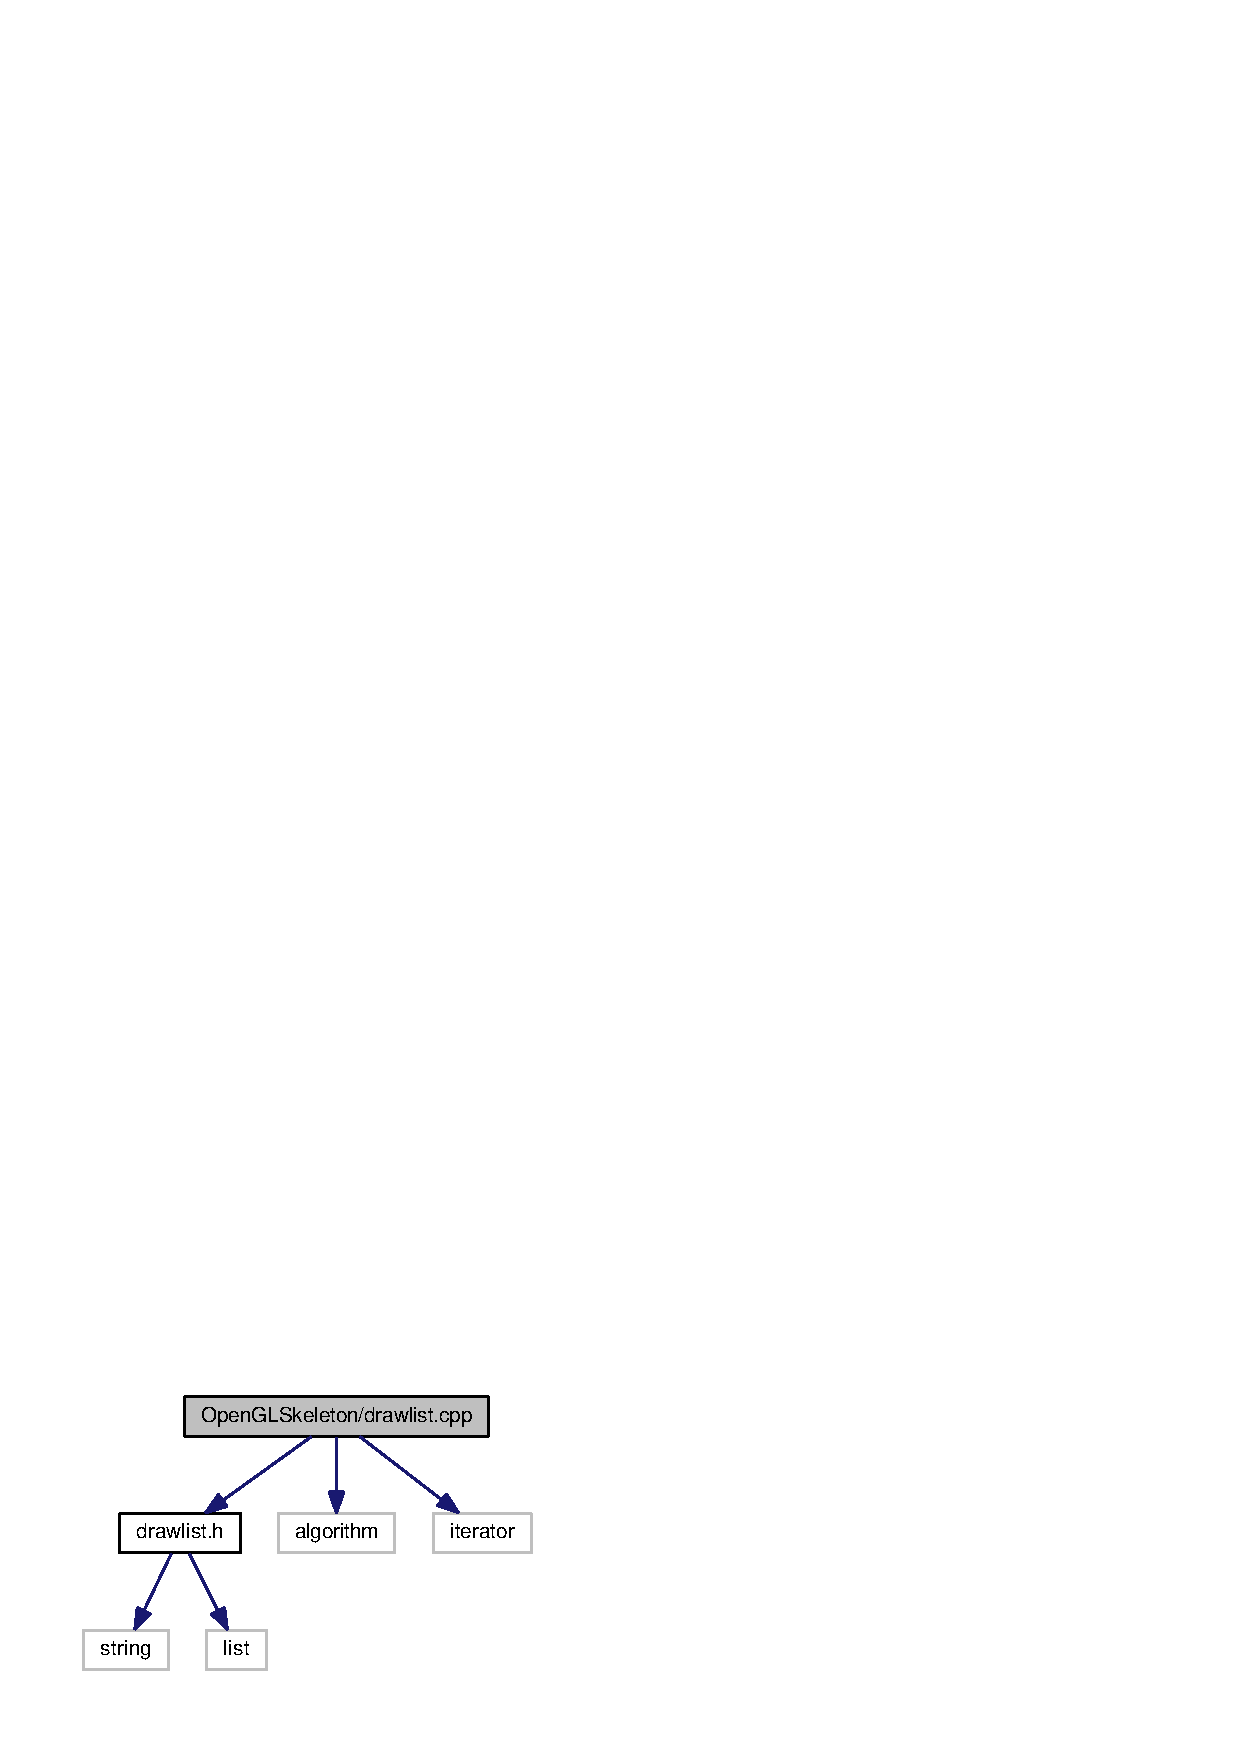
\includegraphics[width=295pt]{drawlist_8cpp__incl}
\end{center}
\end{figure}
\subsection*{Functions}
\begin{DoxyCompactItemize}
\item 
Draw\+List\+::iterator \hyperlink{drawlist_8cpp_a45b945c9a1a268e31ceb456e2cf5115c}{find\+Drawable} (\hyperlink{drawlist_8h_a4dd7049762619e3d87a40c5305bbbfb2}{Draw\+List} \&list, const std\+::string \&name)
\end{DoxyCompactItemize}


\subsection{Function Documentation}
\index{drawlist.\+cpp@{drawlist.\+cpp}!find\+Drawable@{find\+Drawable}}
\index{find\+Drawable@{find\+Drawable}!drawlist.\+cpp@{drawlist.\+cpp}}
\subsubsection[{\texorpdfstring{find\+Drawable(\+Draw\+List \&list, const std\+::string \&name)}{findDrawable(DrawList &list, const std::string &name)}}]{\setlength{\rightskip}{0pt plus 5cm}Draw\+List\+::iterator find\+Drawable (
\begin{DoxyParamCaption}
\item[{{\bf Draw\+List} \&}]{list, }
\item[{const std\+::string \&}]{name}
\end{DoxyParamCaption}
)}\hypertarget{drawlist_8cpp_a45b945c9a1a268e31ceb456e2cf5115c}{}\label{drawlist_8cpp_a45b945c9a1a268e31ceb456e2cf5115c}

\hypertarget{drawlist_8h}{}\section{Open\+G\+L\+Skeleton/drawlist.h File Reference}
\label{drawlist_8h}\index{Open\+G\+L\+Skeleton/drawlist.\+h@{Open\+G\+L\+Skeleton/drawlist.\+h}}
{\ttfamily \#include $<$string$>$}\\*
{\ttfamily \#include $<$list$>$}\\*
Include dependency graph for drawlist.\+h\+:\nopagebreak
\begin{figure}[H]
\begin{center}
\leavevmode
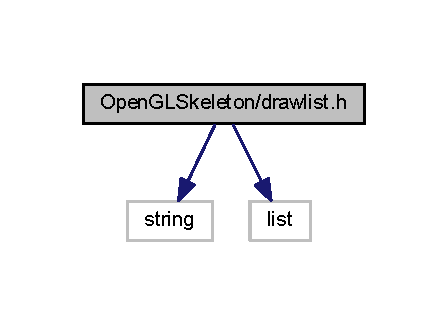
\includegraphics[width=215pt]{drawlist_8h__incl}
\end{center}
\end{figure}
This graph shows which files directly or indirectly include this file\+:\nopagebreak
\begin{figure}[H]
\begin{center}
\leavevmode
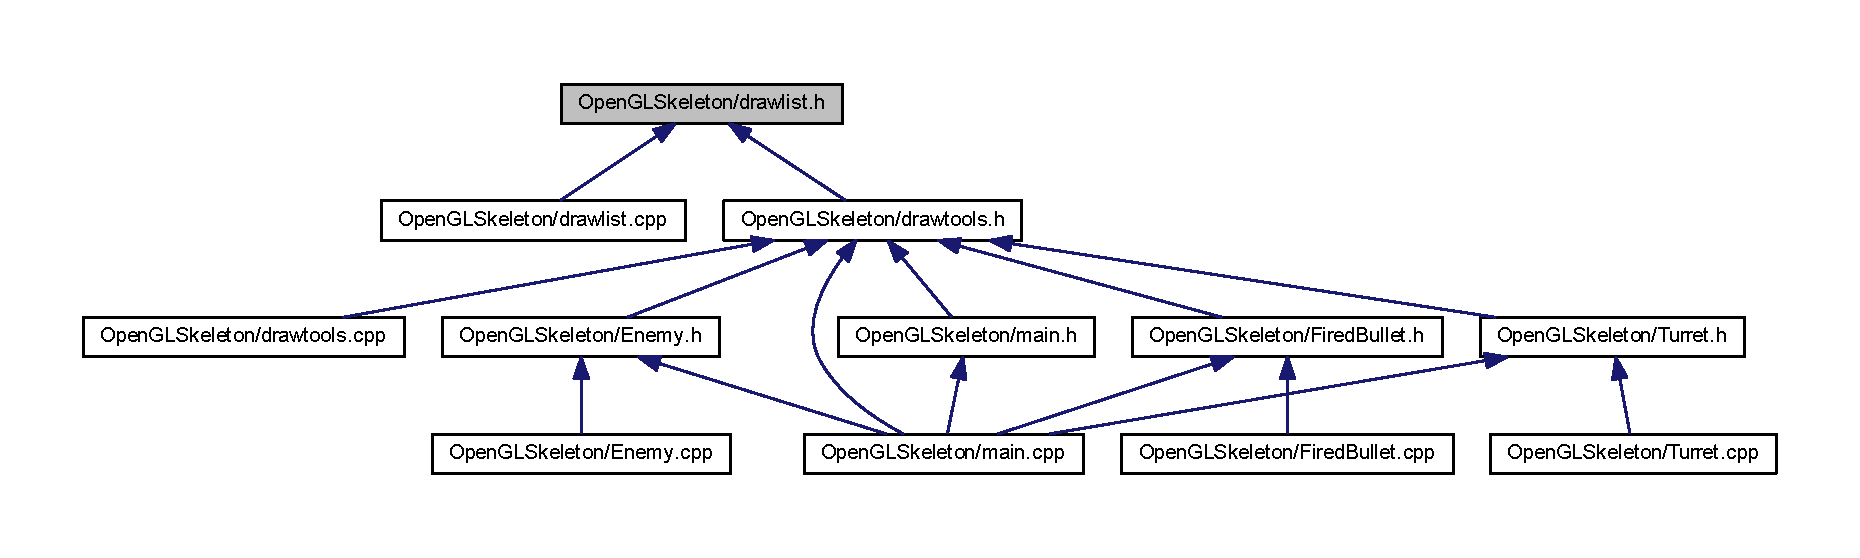
\includegraphics[width=350pt]{drawlist_8h__dep__incl}
\end{center}
\end{figure}
\subsection*{Classes}
\begin{DoxyCompactItemize}
\item 
class \hyperlink{class_drawable}{Drawable}
\end{DoxyCompactItemize}
\subsection*{Typedefs}
\begin{DoxyCompactItemize}
\item 
using \hyperlink{drawlist_8h_a4dd7049762619e3d87a40c5305bbbfb2}{Draw\+List} = std\+::list$<$ \hyperlink{class_drawable}{Drawable} $\ast$ $>$
\end{DoxyCompactItemize}
\subsection*{Functions}
\begin{DoxyCompactItemize}
\item 
Draw\+List\+::iterator \hyperlink{drawlist_8h_a45b945c9a1a268e31ceb456e2cf5115c}{find\+Drawable} (\hyperlink{drawlist_8h_a4dd7049762619e3d87a40c5305bbbfb2}{Draw\+List} \&list, const std\+::string \&name)
\end{DoxyCompactItemize}


\subsection{Typedef Documentation}
\index{drawlist.\+h@{drawlist.\+h}!Draw\+List@{Draw\+List}}
\index{Draw\+List@{Draw\+List}!drawlist.\+h@{drawlist.\+h}}
\subsubsection[{\texorpdfstring{Draw\+List}{DrawList}}]{\setlength{\rightskip}{0pt plus 5cm}using {\bf Draw\+List} =  std\+::list$<${\bf Drawable}$\ast$$>$}\hypertarget{drawlist_8h_a4dd7049762619e3d87a40c5305bbbfb2}{}\label{drawlist_8h_a4dd7049762619e3d87a40c5305bbbfb2}


\subsection{Function Documentation}
\index{drawlist.\+h@{drawlist.\+h}!find\+Drawable@{find\+Drawable}}
\index{find\+Drawable@{find\+Drawable}!drawlist.\+h@{drawlist.\+h}}
\subsubsection[{\texorpdfstring{find\+Drawable(\+Draw\+List \&list, const std\+::string \&name)}{findDrawable(DrawList &list, const std::string &name)}}]{\setlength{\rightskip}{0pt plus 5cm}Draw\+List\+::iterator find\+Drawable (
\begin{DoxyParamCaption}
\item[{{\bf Draw\+List} \&}]{list, }
\item[{const std\+::string \&}]{name}
\end{DoxyParamCaption}
)}\hypertarget{drawlist_8h_a45b945c9a1a268e31ceb456e2cf5115c}{}\label{drawlist_8h_a45b945c9a1a268e31ceb456e2cf5115c}

\hypertarget{drawtools_8cpp}{}\section{Open\+G\+L\+Skeleton/drawtools.cpp File Reference}
\label{drawtools_8cpp}\index{Open\+G\+L\+Skeleton/drawtools.\+cpp@{Open\+G\+L\+Skeleton/drawtools.\+cpp}}
{\ttfamily \#include $<$iostream$>$}\\*
{\ttfamily \#include $<$iomanip$>$}\\*
{\ttfamily \#include $<$string.\+h$>$}\\*
{\ttfamily \#include \char`\"{}glut.\+h\char`\"{}}\\*
{\ttfamily \#include \char`\"{}drawtools.\+h\char`\"{}}\\*
{\ttfamily \#include $<$math.\+h$>$}\\*
Include dependency graph for drawtools.\+cpp\+:
\nopagebreak
\begin{figure}[H]
\begin{center}
\leavevmode
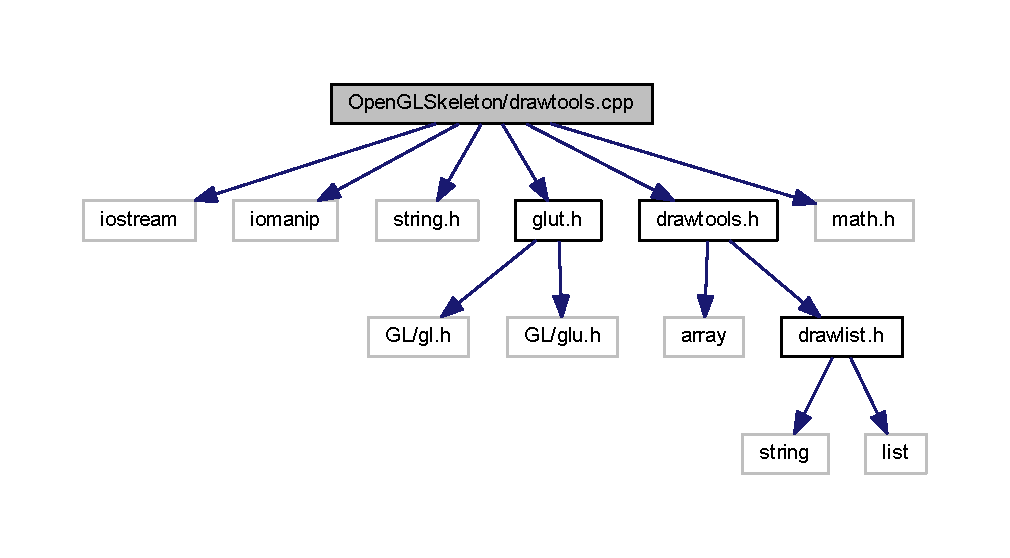
\includegraphics[width=350pt]{drawtools_8cpp__incl}
\end{center}
\end{figure}
\subsection*{Macros}
\begin{DoxyCompactItemize}
\item 
\#define \hyperlink{drawtools_8cpp_a525335710b53cb064ca56b936120431e}{\+\_\+\+U\+S\+E\+\_\+\+M\+A\+T\+H\+\_\+\+D\+E\+F\+I\+N\+ES}
\end{DoxyCompactItemize}


\subsection{Macro Definition Documentation}
\index{drawtools.\+cpp@{drawtools.\+cpp}!\+\_\+\+U\+S\+E\+\_\+\+M\+A\+T\+H\+\_\+\+D\+E\+F\+I\+N\+ES@{\+\_\+\+U\+S\+E\+\_\+\+M\+A\+T\+H\+\_\+\+D\+E\+F\+I\+N\+ES}}
\index{\+\_\+\+U\+S\+E\+\_\+\+M\+A\+T\+H\+\_\+\+D\+E\+F\+I\+N\+ES@{\+\_\+\+U\+S\+E\+\_\+\+M\+A\+T\+H\+\_\+\+D\+E\+F\+I\+N\+ES}!drawtools.\+cpp@{drawtools.\+cpp}}
\subsubsection[{\texorpdfstring{\+\_\+\+U\+S\+E\+\_\+\+M\+A\+T\+H\+\_\+\+D\+E\+F\+I\+N\+ES}{_USE_MATH_DEFINES}}]{\setlength{\rightskip}{0pt plus 5cm}\#define \+\_\+\+U\+S\+E\+\_\+\+M\+A\+T\+H\+\_\+\+D\+E\+F\+I\+N\+ES}\hypertarget{drawtools_8cpp_a525335710b53cb064ca56b936120431e}{}\label{drawtools_8cpp_a525335710b53cb064ca56b936120431e}

\hypertarget{drawtools_8h}{}\section{Open\+G\+L\+Skeleton/drawtools.h File Reference}
\label{drawtools_8h}\index{Open\+G\+L\+Skeleton/drawtools.\+h@{Open\+G\+L\+Skeleton/drawtools.\+h}}
{\ttfamily \#include $<$array$>$}\\*
{\ttfamily \#include \char`\"{}drawlist.\+h\char`\"{}}\\*
Include dependency graph for drawtools.\+h\+:
% FIG 0
This graph shows which files directly or indirectly include this file\+:
% FIG 1
\subsection*{Classes}
\begin{DoxyCompactItemize}
\item 
class \hyperlink{class_point}{Point$<$ T $>$}
\item 
struct \hyperlink{struct_color}{Color}
\item 
class \hyperlink{class_pixel}{Pixel}
\item 
class \hyperlink{class_line}{Line}
\item 
class \hyperlink{class_circle}{Circle}
\item 
class \hyperlink{class_sqaure}{Sqaure}
\item 
class \hyperlink{class_text}{Text}
\end{DoxyCompactItemize}
\subsection*{Typedefs}
\begin{DoxyCompactItemize}
\item 
using \hyperlink{drawtools_8h_aca011a8a706ad4f0b3d267cf3b099fac}{PointI} = \hyperlink{class_point}{Point}$<$ int $>$
\item 
using \hyperlink{drawtools_8h_adc4a66bcb59b74164130ed47cb387ec3}{PointF} = \hyperlink{class_point}{Point}$<$ float $>$
\end{DoxyCompactItemize}


\subsection{Typedef Documentation}
\index{drawtools.\+h@{drawtools.\+h}!PointF@{PointF}}
\index{PointF@{PointF}!drawtools.\+h@{drawtools.\+h}}
\subsubsection[{\texorpdfstring{PointF}{PointF}}]{\setlength{\rightskip}{0pt plus 5cm}using {\bf PointF} =  {\bf Point}$<$float$>$}\hypertarget{drawtools_8h_adc4a66bcb59b74164130ed47cb387ec3}{}\label{drawtools_8h_adc4a66bcb59b74164130ed47cb387ec3}
\index{drawtools.\+h@{drawtools.\+h}!PointI@{PointI}}
\index{PointI@{PointI}!drawtools.\+h@{drawtools.\+h}}
\subsubsection[{\texorpdfstring{PointI}{PointI}}]{\setlength{\rightskip}{0pt plus 5cm}using {\bf PointI} =  {\bf Point}$<$int$>$}\hypertarget{drawtools_8h_aca011a8a706ad4f0b3d267cf3b099fac}{}\label{drawtools_8h_aca011a8a706ad4f0b3d267cf3b099fac}

\hypertarget{_enemy_8cpp}{}\section{Open\+G\+L\+Skeleton/\+Enemy.cpp File Reference}
\label{_enemy_8cpp}\index{Open\+G\+L\+Skeleton/\+Enemy.\+cpp@{Open\+G\+L\+Skeleton/\+Enemy.\+cpp}}
{\ttfamily \#include \char`\"{}Enemy.\+h\char`\"{}}\\*
{\ttfamily \#include $<$iostream$>$}\\*
Include dependency graph for Enemy.\+cpp\+:\nopagebreak
\begin{figure}[H]
\begin{center}
\leavevmode
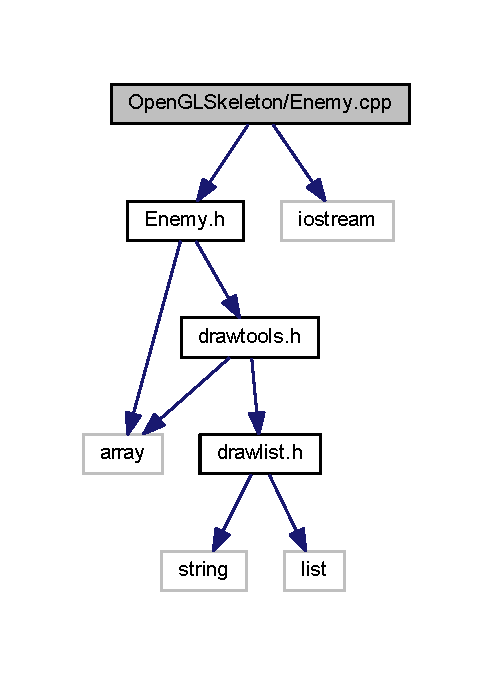
\includegraphics[width=237pt]{_enemy_8cpp__incl}
\end{center}
\end{figure}
\subsection*{Variables}
\begin{DoxyCompactItemize}
\item 
int \hyperlink{_enemy_8cpp_aad462966ed963f892117056de1eba502}{Count} = 1
\end{DoxyCompactItemize}


\subsection{Variable Documentation}
\index{Enemy.\+cpp@{Enemy.\+cpp}!Count@{Count}}
\index{Count@{Count}!Enemy.\+cpp@{Enemy.\+cpp}}
\subsubsection[{\texorpdfstring{Count}{Count}}]{\setlength{\rightskip}{0pt plus 5cm}int Count = 1}\hypertarget{_enemy_8cpp_aad462966ed963f892117056de1eba502}{}\label{_enemy_8cpp_aad462966ed963f892117056de1eba502}

\hypertarget{_enemy_8h}{}\section{Open\+G\+L\+Skeleton/\+Enemy.h File Reference}
\label{_enemy_8h}\index{Open\+G\+L\+Skeleton/\+Enemy.\+h@{Open\+G\+L\+Skeleton/\+Enemy.\+h}}
{\ttfamily \#include $<$array$>$}\\*
{\ttfamily \#include \char`\"{}drawtools.\+h\char`\"{}}\\*
Include dependency graph for Enemy.\+h\+:
% FIG 0
This graph shows which files directly or indirectly include this file\+:
% FIG 1
\subsection*{Classes}
\begin{DoxyCompactItemize}
\item 
class \hyperlink{class_enemy}{Enemy}
\end{DoxyCompactItemize}

\section{Open\+G\+L\+Skeleton/\+Fired\+Bullet.cpp File Reference}
\label{_fired_bullet_8cpp}\index{Open\+G\+L\+Skeleton/\+Fired\+Bullet.\+cpp@{Open\+G\+L\+Skeleton/\+Fired\+Bullet.\+cpp}}
{\ttfamily \#include \char`\"{}Fired\+Bullet.\+h\char`\"{}}\\*
{\ttfamily \#include $<$iostream$>$}\\*
{\ttfamily \#include $<$string$>$}\\*
Include dependency graph for Fired\+Bullet.\+cpp\+:
% FIG 0
\subsection*{Variables}
\begin{DoxyCompactItemize}
\item 
int {\bf Count2} = 0
\end{DoxyCompactItemize}


\subsection{Variable Documentation}
\index{Fired\+Bullet.\+cpp@{Fired\+Bullet.\+cpp}!Count2@{Count2}}
\index{Count2@{Count2}!Fired\+Bullet.\+cpp@{Fired\+Bullet.\+cpp}}
\subsubsection[{Count2}]{\setlength{\rightskip}{0pt plus 5cm}int Count2 = 0}\label{_fired_bullet_8cpp_a1018fd1d06f9728b1adae77ad969ad19}

\section{Open\+G\+L\+Skeleton/\+Fired\+Bullet.h File Reference}
\label{_fired_bullet_8h}\index{Open\+G\+L\+Skeleton/\+Fired\+Bullet.\+h@{Open\+G\+L\+Skeleton/\+Fired\+Bullet.\+h}}
{\ttfamily \#include \char`\"{}drawtools.\+h\char`\"{}}\\*
Include dependency graph for Fired\+Bullet.\+h\+:
% FIG 0
This graph shows which files directly or indirectly include this file\+:
% FIG 1
\subsection*{Classes}
\begin{DoxyCompactItemize}
\item 
class {\bf Fired\+Bullet}
\end{DoxyCompactItemize}
\subsection*{Macros}
\begin{DoxyCompactItemize}
\item 
\#define {\bf F\+I\+R\+E\+D\+B\+U\+L\+L\+E\+T\+\_\+H}
\end{DoxyCompactItemize}


\subsection{Macro Definition Documentation}
\index{Fired\+Bullet.\+h@{Fired\+Bullet.\+h}!F\+I\+R\+E\+D\+B\+U\+L\+L\+E\+T\+\_\+H@{F\+I\+R\+E\+D\+B\+U\+L\+L\+E\+T\+\_\+H}}
\index{F\+I\+R\+E\+D\+B\+U\+L\+L\+E\+T\+\_\+H@{F\+I\+R\+E\+D\+B\+U\+L\+L\+E\+T\+\_\+H}!Fired\+Bullet.\+h@{Fired\+Bullet.\+h}}
\subsubsection[{F\+I\+R\+E\+D\+B\+U\+L\+L\+E\+T\+\_\+H}]{\setlength{\rightskip}{0pt plus 5cm}\#define F\+I\+R\+E\+D\+B\+U\+L\+L\+E\+T\+\_\+H}\label{_fired_bullet_8h_a16f4b748457c5a2f2d2319a585421174}

\hypertarget{glut_8h}{}\section{Open\+G\+L\+Skeleton/glut.h File Reference}
\label{glut_8h}\index{Open\+G\+L\+Skeleton/glut.\+h@{Open\+G\+L\+Skeleton/glut.\+h}}
{\ttfamily \#include $<$G\+L/gl.\+h$>$}\\*
{\ttfamily \#include $<$G\+L/glu.\+h$>$}\\*
Include dependency graph for glut.\+h\+:\nopagebreak
\begin{figure}[H]
\begin{center}
\leavevmode
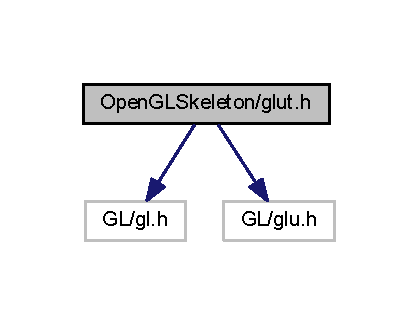
\includegraphics[width=201pt]{glut_8h__incl}
\end{center}
\end{figure}
This graph shows which files directly or indirectly include this file\+:\nopagebreak
\begin{figure}[H]
\begin{center}
\leavevmode
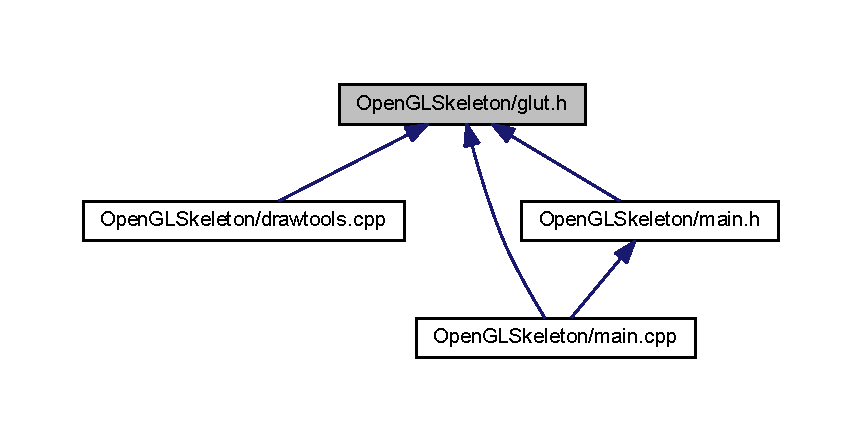
\includegraphics[width=350pt]{glut_8h__dep__incl}
\end{center}
\end{figure}
\subsection*{Macros}
\begin{DoxyCompactItemize}
\item 
\#define \hyperlink{glut_8h_a428a91acf2c2439dc1a257708ee1f805}{A\+P\+I\+E\+N\+T\+RY}
\item 
\#define \hyperlink{glut_8h_aaf538c0b5f6a3d6f0cbf54ff6740f42e}{G\+L\+U\+T\+\_\+\+A\+P\+I\+E\+N\+T\+R\+Y\+\_\+\+D\+E\+F\+I\+N\+ED}
\item 
\#define \hyperlink{glut_8h_ad48a1ae177f90ad8a0ccc92481c664a7}{C\+A\+L\+L\+B\+A\+CK}
\item 
\#define \hyperlink{glut_8h_aaffce4b1257a6919684ac58d7e04342e}{G\+L\+U\+T\+A\+PI}~extern
\item 
\#define \hyperlink{glut_8h_a207caac251f0305666a3d61a71af5fc7}{G\+L\+U\+T\+C\+A\+L\+L\+B\+A\+CK}
\item 
\#define \hyperlink{glut_8h_a2fc3bb51b9f38ac5b0cb7911be9caf94}{G\+L\+U\+T\+\_\+\+A\+P\+I\+\_\+\+V\+E\+R\+S\+I\+ON}~3
\item 
\#define \hyperlink{glut_8h_aa5c483c6696110f8f296009ddc7cefd3}{G\+L\+U\+T\+\_\+\+X\+L\+I\+B\+\_\+\+I\+M\+P\+L\+E\+M\+E\+N\+T\+A\+T\+I\+ON}~15
\item 
\#define \hyperlink{glut_8h_af72a6f59f18e560f3ee70b9feb40eeb5}{G\+L\+U\+T\+\_\+\+R\+GB}~0
\item 
\#define \hyperlink{glut_8h_a9766fe825112d4042a731effa96e9ed7}{G\+L\+U\+T\+\_\+\+R\+G\+BA}~\hyperlink{glut_8h_af72a6f59f18e560f3ee70b9feb40eeb5}{G\+L\+U\+T\+\_\+\+R\+GB}
\item 
\#define \hyperlink{glut_8h_a27cb2be9915eb425610664a7daeec74a}{G\+L\+U\+T\+\_\+\+I\+N\+D\+EX}~1
\item 
\#define \hyperlink{glut_8h_a3d45cc54fd3274143881a0633600709f}{G\+L\+U\+T\+\_\+\+S\+I\+N\+G\+LE}~0
\item 
\#define \hyperlink{glut_8h_a199f7f46cadfb6a94b2b7095f3ff3428}{G\+L\+U\+T\+\_\+\+D\+O\+U\+B\+LE}~2
\item 
\#define \hyperlink{glut_8h_a43896fd591995b08379ec5d945c6b9ca}{G\+L\+U\+T\+\_\+\+A\+C\+C\+UM}~4
\item 
\#define \hyperlink{glut_8h_a2d492a7606bd5c29f2ba12bb194b5866}{G\+L\+U\+T\+\_\+\+A\+L\+P\+HA}~8
\item 
\#define \hyperlink{glut_8h_a82a20e99a815f32f5f936971e2fa5651}{G\+L\+U\+T\+\_\+\+D\+E\+P\+TH}~16
\item 
\#define \hyperlink{glut_8h_af8f7a79dc36c44f922225d9109196403}{G\+L\+U\+T\+\_\+\+S\+T\+E\+N\+C\+IL}~32
\item 
\#define \hyperlink{glut_8h_a3f15e21c2a814e8db3d00ec1e9f58d71}{G\+L\+U\+T\+\_\+\+M\+U\+L\+T\+I\+S\+A\+M\+P\+LE}~128
\item 
\#define \hyperlink{glut_8h_a0cd1ad5ec8468b9a0cdd4158e791dc19}{G\+L\+U\+T\+\_\+\+S\+T\+E\+R\+EO}~256
\item 
\#define \hyperlink{glut_8h_aae79c99329207ad9262f2b3fbe4aa1ee}{G\+L\+U\+T\+\_\+\+L\+U\+M\+I\+N\+A\+N\+CE}~512
\item 
\#define \hyperlink{glut_8h_a889091fa01fbf2f7d4d6f86b5028b54b}{G\+L\+U\+T\+\_\+\+L\+E\+F\+T\+\_\+\+B\+U\+T\+T\+ON}~0
\item 
\#define \hyperlink{glut_8h_a99af895d2ade59903d17dc05167fc2e9}{G\+L\+U\+T\+\_\+\+M\+I\+D\+D\+L\+E\+\_\+\+B\+U\+T\+T\+ON}~1
\item 
\#define \hyperlink{glut_8h_ada993ed7a1ceee11b1c3326b8b15dbf3}{G\+L\+U\+T\+\_\+\+R\+I\+G\+H\+T\+\_\+\+B\+U\+T\+T\+ON}~2
\item 
\#define \hyperlink{glut_8h_a0ff13272cadc7de03287a4c2f1ccd74c}{G\+L\+U\+T\+\_\+\+W\+H\+E\+E\+L\+\_\+\+UP}~3
\item 
\#define \hyperlink{glut_8h_a04012499337ad32ddf797c3be334a9bc}{G\+L\+U\+T\+\_\+\+W\+H\+E\+E\+L\+\_\+\+D\+O\+WN}~4
\item 
\#define \hyperlink{glut_8h_a327b201ceafb47b9f919e3fb60596204}{G\+L\+U\+T\+\_\+\+X\+B\+U\+T\+T\+O\+N1}~5
\item 
\#define \hyperlink{glut_8h_a838389655c877d2495d5cf6de89f0792}{G\+L\+U\+T\+\_\+\+X\+B\+U\+T\+T\+O\+N2}~6
\item 
\#define \hyperlink{glut_8h_a30d72298588fe4f6204e9f6d86f955b3}{G\+L\+U\+T\+\_\+\+D\+O\+WN}~0
\item 
\#define \hyperlink{glut_8h_a1afddf27f2001b4e65470a41bdde30d9}{G\+L\+U\+T\+\_\+\+UP}~1
\item 
\#define \hyperlink{glut_8h_af63cc7b29a12af0955c42dea87829736}{G\+L\+U\+T\+\_\+\+K\+E\+Y\+\_\+\+F1}~1
\item 
\#define \hyperlink{glut_8h_acb72407f62b6cfc4faac1b9d79da2623}{G\+L\+U\+T\+\_\+\+K\+E\+Y\+\_\+\+F2}~2
\item 
\#define \hyperlink{glut_8h_a9680619e50bb1ec577e2e36be50c8b90}{G\+L\+U\+T\+\_\+\+K\+E\+Y\+\_\+\+F3}~3
\item 
\#define \hyperlink{glut_8h_ae8d810517559c68a5f62456d2b77425a}{G\+L\+U\+T\+\_\+\+K\+E\+Y\+\_\+\+F4}~4
\item 
\#define \hyperlink{glut_8h_a996d079f4f3f3a8c7c6a01ca6db9258b}{G\+L\+U\+T\+\_\+\+K\+E\+Y\+\_\+\+F5}~5
\item 
\#define \hyperlink{glut_8h_a14ff110c3b644cf9072d37197fa0a34e}{G\+L\+U\+T\+\_\+\+K\+E\+Y\+\_\+\+F6}~6
\item 
\#define \hyperlink{glut_8h_a0cb22cbc1ac854e2c8a1a5f6ae04665c}{G\+L\+U\+T\+\_\+\+K\+E\+Y\+\_\+\+F7}~7
\item 
\#define \hyperlink{glut_8h_aac707cfc5f4e56de1ea98466be5ea5ad}{G\+L\+U\+T\+\_\+\+K\+E\+Y\+\_\+\+F8}~8
\item 
\#define \hyperlink{glut_8h_aadc9265d666b1bc3827ba25570f18cf4}{G\+L\+U\+T\+\_\+\+K\+E\+Y\+\_\+\+F9}~9
\item 
\#define \hyperlink{glut_8h_aa0945fa7982b39eefa42014700f483c9}{G\+L\+U\+T\+\_\+\+K\+E\+Y\+\_\+\+F10}~10
\item 
\#define \hyperlink{glut_8h_a9ff68b79b29283e2602c936b5c3aefc5}{G\+L\+U\+T\+\_\+\+K\+E\+Y\+\_\+\+F11}~11
\item 
\#define \hyperlink{glut_8h_a29817688a1c9f26fd697d811da48e223}{G\+L\+U\+T\+\_\+\+K\+E\+Y\+\_\+\+F12}~12
\item 
\#define \hyperlink{glut_8h_abb193c04e62c29184751e2055fda89f5}{G\+L\+U\+T\+\_\+\+K\+E\+Y\+\_\+\+L\+E\+FT}~100
\item 
\#define \hyperlink{glut_8h_ada7f412e1ab4f271da990a217aca5b73}{G\+L\+U\+T\+\_\+\+K\+E\+Y\+\_\+\+UP}~101
\item 
\#define \hyperlink{glut_8h_a19beda7d173600127ee540aee53dd081}{G\+L\+U\+T\+\_\+\+K\+E\+Y\+\_\+\+R\+I\+G\+HT}~102
\item 
\#define \hyperlink{glut_8h_acf185aebae7f4bee9d4e95e0e889baa7}{G\+L\+U\+T\+\_\+\+K\+E\+Y\+\_\+\+D\+O\+WN}~103
\item 
\#define \hyperlink{glut_8h_a28093e59b0ac1a1a25790fe45413db52}{G\+L\+U\+T\+\_\+\+K\+E\+Y\+\_\+\+P\+A\+G\+E\+\_\+\+UP}~104
\item 
\#define \hyperlink{glut_8h_ada3e1475a629486163f75867350cddb4}{G\+L\+U\+T\+\_\+\+K\+E\+Y\+\_\+\+P\+A\+G\+E\+\_\+\+D\+O\+WN}~105
\item 
\#define \hyperlink{glut_8h_adf559535a9b6a83e60e19b503cbd8267}{G\+L\+U\+T\+\_\+\+K\+E\+Y\+\_\+\+H\+O\+ME}~106
\item 
\#define \hyperlink{glut_8h_a8e90fbfbeea6c49891e022e07c9de056}{G\+L\+U\+T\+\_\+\+K\+E\+Y\+\_\+\+E\+ND}~107
\item 
\#define \hyperlink{glut_8h_a73eebf3d2d1ccd5ce867a608e0e2a751}{G\+L\+U\+T\+\_\+\+K\+E\+Y\+\_\+\+I\+N\+S\+E\+RT}~108
\item 
\#define \hyperlink{glut_8h_af581f17fc90ea8883fb28a0ec26c889d}{G\+L\+U\+T\+\_\+\+L\+E\+FT}~0
\item 
\#define \hyperlink{glut_8h_a2442615bbc9f806206f3c0334fe73181}{G\+L\+U\+T\+\_\+\+E\+N\+T\+E\+R\+ED}~1
\item 
\#define \hyperlink{glut_8h_a52f844a404adac32c0754da123b1d471}{G\+L\+U\+T\+\_\+\+M\+E\+N\+U\+\_\+\+N\+O\+T\+\_\+\+I\+N\+\_\+\+U\+SE}~0
\item 
\#define \hyperlink{glut_8h_a4559f0cb6963c422c3cd87b998e42f4b}{G\+L\+U\+T\+\_\+\+M\+E\+N\+U\+\_\+\+I\+N\+\_\+\+U\+SE}~1
\item 
\#define \hyperlink{glut_8h_a64a22710d37c8674704e90fc2010c950}{G\+L\+U\+T\+\_\+\+N\+O\+T\+\_\+\+V\+I\+S\+I\+B\+LE}~0
\item 
\#define \hyperlink{glut_8h_a7037cf658e4512296cef256c020f0fdb}{G\+L\+U\+T\+\_\+\+V\+I\+S\+I\+B\+LE}~1
\item 
\#define \hyperlink{glut_8h_a68c1ead3367a836f1f8f59641fc2b299}{G\+L\+U\+T\+\_\+\+H\+I\+D\+D\+EN}~0
\item 
\#define \hyperlink{glut_8h_ab2c0c0640fe1157c8eb59fcb7d62e108}{G\+L\+U\+T\+\_\+\+F\+U\+L\+L\+Y\+\_\+\+R\+E\+T\+A\+I\+N\+ED}~1
\item 
\#define \hyperlink{glut_8h_a0382440b8fd65823c51bfc9847d06f7c}{G\+L\+U\+T\+\_\+\+P\+A\+R\+T\+I\+A\+L\+L\+Y\+\_\+\+R\+E\+T\+A\+I\+N\+ED}~2
\item 
\#define \hyperlink{glut_8h_a5ba05621d2288349a25b82f3295425cf}{G\+L\+U\+T\+\_\+\+F\+U\+L\+L\+Y\+\_\+\+C\+O\+V\+E\+R\+ED}~3
\item 
\#define \hyperlink{glut_8h_aef848f2d576af78e59be7201d45ea4ec}{G\+L\+U\+T\+\_\+\+R\+ED}~0
\item 
\#define \hyperlink{glut_8h_a3e31e620fa555ee3a0667a04827a7d0c}{G\+L\+U\+T\+\_\+\+G\+R\+E\+EN}~1
\item 
\#define \hyperlink{glut_8h_a074d38dfa1098ff10e371902adb0b8ed}{G\+L\+U\+T\+\_\+\+B\+L\+UE}~2
\item 
\#define \hyperlink{glut_8h_a8c868e8790fc8d62e4d6a3923cb2c007}{G\+L\+U\+T\+\_\+\+S\+T\+R\+O\+K\+E\+\_\+\+R\+O\+M\+AN}~(\&\hyperlink{glut_8h_a1661489685de33b42abe1412e2de1bfa}{glut\+Stroke\+Roman})
\item 
\#define \hyperlink{glut_8h_a6d845b04aa17e263c96e07b95872b404}{G\+L\+U\+T\+\_\+\+S\+T\+R\+O\+K\+E\+\_\+\+M\+O\+N\+O\+\_\+\+R\+O\+M\+AN}~(\&\hyperlink{glut_8h_a0c0898e93370396ca36cb4f138212612}{glut\+Stroke\+Mono\+Roman})
\item 
\#define \hyperlink{glut_8h_abd22ae2e12348f35e2822d9e23aa50de}{G\+L\+U\+T\+\_\+\+B\+I\+T\+M\+A\+P\+\_\+9\+\_\+\+B\+Y\+\_\+15}~(\&\hyperlink{glut_8h_ad22ab8ca3c4739db72045ba3f271c0fc}{glut\+Bitmap9\+By15})
\item 
\#define \hyperlink{glut_8h_a19b58769a20dd6fb34e6b5a2ecd42c2a}{G\+L\+U\+T\+\_\+\+B\+I\+T\+M\+A\+P\+\_\+8\+\_\+\+B\+Y\+\_\+13}~(\&\hyperlink{glut_8h_a8f2e1183e57f784e398b9d4e36cf6bd5}{glut\+Bitmap8\+By13})
\item 
\#define \hyperlink{glut_8h_ab570839ce3413815606992f14dc9a9d4}{G\+L\+U\+T\+\_\+\+B\+I\+T\+M\+A\+P\+\_\+\+T\+I\+M\+E\+S\+\_\+\+R\+O\+M\+A\+N\+\_\+10}~(\&\hyperlink{glut_8h_a8011e129e2c15dc5521d961ac46c1993}{glut\+Bitmap\+Times\+Roman10})
\item 
\#define \hyperlink{glut_8h_a3a5b5a835fb02e6a681b8092fe25cc8c}{G\+L\+U\+T\+\_\+\+B\+I\+T\+M\+A\+P\+\_\+\+T\+I\+M\+E\+S\+\_\+\+R\+O\+M\+A\+N\+\_\+24}~(\&\hyperlink{glut_8h_af52b68752d10ea87ec2b0816158bc548}{glut\+Bitmap\+Times\+Roman24})
\item 
\#define \hyperlink{glut_8h_ac11db7b9af4fb9c1b2e37be43728f34d}{G\+L\+U\+T\+\_\+\+B\+I\+T\+M\+A\+P\+\_\+\+H\+E\+L\+V\+E\+T\+I\+C\+A\+\_\+10}~(\&\hyperlink{glut_8h_a6d57e0271fd48ca0697689cbf4e13d89}{glut\+Bitmap\+Helvetica10})
\item 
\#define \hyperlink{glut_8h_a7148f404947be386e4a4cbd2ec84d15e}{G\+L\+U\+T\+\_\+\+B\+I\+T\+M\+A\+P\+\_\+\+H\+E\+L\+V\+E\+T\+I\+C\+A\+\_\+12}~(\&\hyperlink{glut_8h_af1da4ef00afcd5348c5ec67092986bf4}{glut\+Bitmap\+Helvetica12})
\item 
\#define \hyperlink{glut_8h_aa2733cf18efd2cf595fe00e2eef5fd46}{G\+L\+U\+T\+\_\+\+B\+I\+T\+M\+A\+P\+\_\+\+H\+E\+L\+V\+E\+T\+I\+C\+A\+\_\+18}~(\&\hyperlink{glut_8h_afeeccbc1d58560fe99b298495fb84d3a}{glut\+Bitmap\+Helvetica18})
\item 
\#define \hyperlink{glut_8h_afd840a4550534860f84493c99889444c}{G\+L\+U\+T\+\_\+\+W\+I\+N\+D\+O\+W\+\_\+X}~((G\+Lenum) 100)
\item 
\#define \hyperlink{glut_8h_af96c91347385211c5fc8c4e480e724bf}{G\+L\+U\+T\+\_\+\+W\+I\+N\+D\+O\+W\+\_\+Y}~((G\+Lenum) 101)
\item 
\#define \hyperlink{glut_8h_a0f3be11b8fee187ebb7404d963c7d31e}{G\+L\+U\+T\+\_\+\+W\+I\+N\+D\+O\+W\+\_\+\+W\+I\+D\+TH}~((G\+Lenum) 102)
\item 
\#define \hyperlink{glut_8h_aa59ab5701b62782baab5d05e71d646ab}{G\+L\+U\+T\+\_\+\+W\+I\+N\+D\+O\+W\+\_\+\+H\+E\+I\+G\+HT}~((G\+Lenum) 103)
\item 
\#define \hyperlink{glut_8h_a3a9c3935e7ddf12b8a70a7f5df3626c1}{G\+L\+U\+T\+\_\+\+W\+I\+N\+D\+O\+W\+\_\+\+B\+U\+F\+F\+E\+R\+\_\+\+S\+I\+ZE}~((G\+Lenum) 104)
\item 
\#define \hyperlink{glut_8h_adb9314f66a8f824f71322454decee406}{G\+L\+U\+T\+\_\+\+W\+I\+N\+D\+O\+W\+\_\+\+S\+T\+E\+N\+C\+I\+L\+\_\+\+S\+I\+ZE}~((G\+Lenum) 105)
\item 
\#define \hyperlink{glut_8h_a75550c7d5af9c48876449d0a1a2cb399}{G\+L\+U\+T\+\_\+\+W\+I\+N\+D\+O\+W\+\_\+\+D\+E\+P\+T\+H\+\_\+\+S\+I\+ZE}~((G\+Lenum) 106)
\item 
\#define \hyperlink{glut_8h_a44509f72b4642ec2eec721327cd1fb7f}{G\+L\+U\+T\+\_\+\+W\+I\+N\+D\+O\+W\+\_\+\+R\+E\+D\+\_\+\+S\+I\+ZE}~((G\+Lenum) 107)
\item 
\#define \hyperlink{glut_8h_a3ab3056f0fe86d066fa89af6cde18ed8}{G\+L\+U\+T\+\_\+\+W\+I\+N\+D\+O\+W\+\_\+\+G\+R\+E\+E\+N\+\_\+\+S\+I\+ZE}~((G\+Lenum) 108)
\item 
\#define \hyperlink{glut_8h_abdf4e98e2114bc0707239ea8019a9be9}{G\+L\+U\+T\+\_\+\+W\+I\+N\+D\+O\+W\+\_\+\+B\+L\+U\+E\+\_\+\+S\+I\+ZE}~((G\+Lenum) 109)
\item 
\#define \hyperlink{glut_8h_a57d82d9d76b5c6f5f8e7d3466609399e}{G\+L\+U\+T\+\_\+\+W\+I\+N\+D\+O\+W\+\_\+\+A\+L\+P\+H\+A\+\_\+\+S\+I\+ZE}~((G\+Lenum) 110)
\item 
\#define \hyperlink{glut_8h_a2110a2aecd5d4ad7a104a0b9477a3629}{G\+L\+U\+T\+\_\+\+W\+I\+N\+D\+O\+W\+\_\+\+A\+C\+C\+U\+M\+\_\+\+R\+E\+D\+\_\+\+S\+I\+ZE}~((G\+Lenum) 111)
\item 
\#define \hyperlink{glut_8h_aafbd9803c6c09cefc820bc0d9646c4a4}{G\+L\+U\+T\+\_\+\+W\+I\+N\+D\+O\+W\+\_\+\+A\+C\+C\+U\+M\+\_\+\+G\+R\+E\+E\+N\+\_\+\+S\+I\+ZE}~((G\+Lenum) 112)
\item 
\#define \hyperlink{glut_8h_a74844f3c9ea2afa20a81638a45049ad9}{G\+L\+U\+T\+\_\+\+W\+I\+N\+D\+O\+W\+\_\+\+A\+C\+C\+U\+M\+\_\+\+B\+L\+U\+E\+\_\+\+S\+I\+ZE}~((G\+Lenum) 113)
\item 
\#define \hyperlink{glut_8h_a253794e453f452508d170c62ac34e638}{G\+L\+U\+T\+\_\+\+W\+I\+N\+D\+O\+W\+\_\+\+A\+C\+C\+U\+M\+\_\+\+A\+L\+P\+H\+A\+\_\+\+S\+I\+ZE}~((G\+Lenum) 114)
\item 
\#define \hyperlink{glut_8h_a9209d34d3fb3805e395878acd78e2f02}{G\+L\+U\+T\+\_\+\+W\+I\+N\+D\+O\+W\+\_\+\+D\+O\+U\+B\+L\+E\+B\+U\+F\+F\+ER}~((G\+Lenum) 115)
\item 
\#define \hyperlink{glut_8h_a3b538c911c396c95b24c4a59be27ab3b}{G\+L\+U\+T\+\_\+\+W\+I\+N\+D\+O\+W\+\_\+\+R\+G\+BA}~((G\+Lenum) 116)
\item 
\#define \hyperlink{glut_8h_a724c63b0ab39db859a2a3a7b1212db8f}{G\+L\+U\+T\+\_\+\+W\+I\+N\+D\+O\+W\+\_\+\+P\+A\+R\+E\+NT}~((G\+Lenum) 117)
\item 
\#define \hyperlink{glut_8h_a3c4cc1eb509c112a06d2b727b4a4845a}{G\+L\+U\+T\+\_\+\+W\+I\+N\+D\+O\+W\+\_\+\+N\+U\+M\+\_\+\+C\+H\+I\+L\+D\+R\+EN}~((G\+Lenum) 118)
\item 
\#define \hyperlink{glut_8h_a02eae1e68c788e930924f1b1f36f5169}{G\+L\+U\+T\+\_\+\+W\+I\+N\+D\+O\+W\+\_\+\+C\+O\+L\+O\+R\+M\+A\+P\+\_\+\+S\+I\+ZE}~((G\+Lenum) 119)
\item 
\#define \hyperlink{glut_8h_ab45baab849e18a8dc86cb230d8582436}{G\+L\+U\+T\+\_\+\+W\+I\+N\+D\+O\+W\+\_\+\+N\+U\+M\+\_\+\+S\+A\+M\+P\+L\+ES}~((G\+Lenum) 120)
\item 
\#define \hyperlink{glut_8h_a37c7f9ceeb75ab4f4a02da02b0f50d4b}{G\+L\+U\+T\+\_\+\+W\+I\+N\+D\+O\+W\+\_\+\+S\+T\+E\+R\+EO}~((G\+Lenum) 121)
\item 
\#define \hyperlink{glut_8h_a887e0ff085061db7bf3daaa3d079f7e4}{G\+L\+U\+T\+\_\+\+W\+I\+N\+D\+O\+W\+\_\+\+C\+U\+R\+S\+OR}~((G\+Lenum) 122)
\item 
\#define \hyperlink{glut_8h_a6b65bdffe7a0842ddeb96e7df24bc052}{G\+L\+U\+T\+\_\+\+S\+C\+R\+E\+E\+N\+\_\+\+W\+I\+D\+TH}~((G\+Lenum) 200)
\item 
\#define \hyperlink{glut_8h_ab886a3d74de701fd9a6d225f440d7600}{G\+L\+U\+T\+\_\+\+S\+C\+R\+E\+E\+N\+\_\+\+H\+E\+I\+G\+HT}~((G\+Lenum) 201)
\item 
\#define \hyperlink{glut_8h_a118f8271d40bf215c6893e2b78651c0c}{G\+L\+U\+T\+\_\+\+S\+C\+R\+E\+E\+N\+\_\+\+W\+I\+D\+T\+H\+\_\+\+MM}~((G\+Lenum) 202)
\item 
\#define \hyperlink{glut_8h_a48916f3cd0b6a8805b4de3c72efad0e3}{G\+L\+U\+T\+\_\+\+S\+C\+R\+E\+E\+N\+\_\+\+H\+E\+I\+G\+H\+T\+\_\+\+MM}~((G\+Lenum) 203)
\item 
\#define \hyperlink{glut_8h_a81c9244e4286cf9ef3326e8197e3aae0}{G\+L\+U\+T\+\_\+\+M\+E\+N\+U\+\_\+\+N\+U\+M\+\_\+\+I\+T\+E\+MS}~((G\+Lenum) 300)
\item 
\#define \hyperlink{glut_8h_a679ca1a9f339a7cbced60f89e0fc8925}{G\+L\+U\+T\+\_\+\+D\+I\+S\+P\+L\+A\+Y\+\_\+\+M\+O\+D\+E\+\_\+\+P\+O\+S\+S\+I\+B\+LE}~((G\+Lenum) 400)
\item 
\#define \hyperlink{glut_8h_a7627ed8c6224d6389f30cabcf7cda967}{G\+L\+U\+T\+\_\+\+I\+N\+I\+T\+\_\+\+W\+I\+N\+D\+O\+W\+\_\+X}~((G\+Lenum) 500)
\item 
\#define \hyperlink{glut_8h_a8c3a6de14aa9b522d6a9c4993da064fb}{G\+L\+U\+T\+\_\+\+I\+N\+I\+T\+\_\+\+W\+I\+N\+D\+O\+W\+\_\+Y}~((G\+Lenum) 501)
\item 
\#define \hyperlink{glut_8h_a792dacbe7ae1d6d0cda0f1cc8fce6e9e}{G\+L\+U\+T\+\_\+\+I\+N\+I\+T\+\_\+\+W\+I\+N\+D\+O\+W\+\_\+\+W\+I\+D\+TH}~((G\+Lenum) 502)
\item 
\#define \hyperlink{glut_8h_abf9ae3b75dae2531ade9cec68b0da41a}{G\+L\+U\+T\+\_\+\+I\+N\+I\+T\+\_\+\+W\+I\+N\+D\+O\+W\+\_\+\+H\+E\+I\+G\+HT}~((G\+Lenum) 503)
\item 
\#define \hyperlink{glut_8h_a9f12a56b38000f6bc663aed7f5dbf803}{G\+L\+U\+T\+\_\+\+I\+N\+I\+T\+\_\+\+D\+I\+S\+P\+L\+A\+Y\+\_\+\+M\+O\+DE}~((G\+Lenum) 504)
\item 
\#define \hyperlink{glut_8h_a9a38f125fd6a5ca22bfbae59d5654146}{G\+L\+U\+T\+\_\+\+E\+L\+A\+P\+S\+E\+D\+\_\+\+T\+I\+ME}~((G\+Lenum) 700)
\item 
\#define \hyperlink{glut_8h_a8d884b32318ca281266952db0cb16ac9}{G\+L\+U\+T\+\_\+\+W\+I\+N\+D\+O\+W\+\_\+\+F\+O\+R\+M\+A\+T\+\_\+\+ID}~((G\+Lenum) 123)
\item 
\#define \hyperlink{glut_8h_afc9f178dce8da5d750839f8607986706}{G\+L\+U\+T\+\_\+\+H\+A\+S\+\_\+\+K\+E\+Y\+B\+O\+A\+RD}~((G\+Lenum) 600)
\item 
\#define \hyperlink{glut_8h_a4d860760b75e8ba688820a8917f54aa6}{G\+L\+U\+T\+\_\+\+H\+A\+S\+\_\+\+M\+O\+U\+SE}~((G\+Lenum) 601)
\item 
\#define \hyperlink{glut_8h_ac6f10f5ba7fa1db4236ff4350cbece04}{G\+L\+U\+T\+\_\+\+H\+A\+S\+\_\+\+S\+P\+A\+C\+E\+B\+A\+LL}~((G\+Lenum) 602)
\item 
\#define \hyperlink{glut_8h_a118efbf04d3b594b7fca68920254d2fe}{G\+L\+U\+T\+\_\+\+H\+A\+S\+\_\+\+D\+I\+A\+L\+\_\+\+A\+N\+D\+\_\+\+B\+U\+T\+T\+O\+N\+\_\+\+B\+OX}~((G\+Lenum) 603)
\item 
\#define \hyperlink{glut_8h_ab909efdd1d504d879e958b36dedc2173}{G\+L\+U\+T\+\_\+\+H\+A\+S\+\_\+\+T\+A\+B\+L\+ET}~((G\+Lenum) 604)
\item 
\#define \hyperlink{glut_8h_a202d9c83876fe0b87d1af980463caefa}{G\+L\+U\+T\+\_\+\+N\+U\+M\+\_\+\+M\+O\+U\+S\+E\+\_\+\+B\+U\+T\+T\+O\+NS}~((G\+Lenum) 605)
\item 
\#define \hyperlink{glut_8h_aa4ff5141791cc3999281dcdb1fadc4a5}{G\+L\+U\+T\+\_\+\+N\+U\+M\+\_\+\+S\+P\+A\+C\+E\+B\+A\+L\+L\+\_\+\+B\+U\+T\+T\+O\+NS}~((G\+Lenum) 606)
\item 
\#define \hyperlink{glut_8h_af5f59269acd5687125d7c3c7b6e3fd35}{G\+L\+U\+T\+\_\+\+N\+U\+M\+\_\+\+B\+U\+T\+T\+O\+N\+\_\+\+B\+O\+X\+\_\+\+B\+U\+T\+T\+O\+NS}~((G\+Lenum) 607)
\item 
\#define \hyperlink{glut_8h_a494de5ea1c0624bd31f8aa3ea919494b}{G\+L\+U\+T\+\_\+\+N\+U\+M\+\_\+\+D\+I\+A\+LS}~((G\+Lenum) 608)
\item 
\#define \hyperlink{glut_8h_aee4d8f95dfd13e13f762c3a081c6036a}{G\+L\+U\+T\+\_\+\+N\+U\+M\+\_\+\+T\+A\+B\+L\+E\+T\+\_\+\+B\+U\+T\+T\+O\+NS}~((G\+Lenum) 609)
\item 
\#define \hyperlink{glut_8h_a7d1e2be6f8992e6767726ba46662e53c}{G\+L\+U\+T\+\_\+\+D\+E\+V\+I\+C\+E\+\_\+\+I\+G\+N\+O\+R\+E\+\_\+\+K\+E\+Y\+\_\+\+R\+E\+P\+E\+AT}~((G\+Lenum) 610)
\item 
\#define \hyperlink{glut_8h_a162161f62031108981e49e564a80f2ce}{G\+L\+U\+T\+\_\+\+D\+E\+V\+I\+C\+E\+\_\+\+K\+E\+Y\+\_\+\+R\+E\+P\+E\+AT}~((G\+Lenum) 611)
\item 
\#define \hyperlink{glut_8h_a7057c6b4ce201e5022db8eca0654c58a}{G\+L\+U\+T\+\_\+\+H\+A\+S\+\_\+\+J\+O\+Y\+S\+T\+I\+CK}~((G\+Lenum) 612)
\item 
\#define \hyperlink{glut_8h_ad22e11bb01cb47ce949bccdec92795bc}{G\+L\+U\+T\+\_\+\+O\+W\+N\+S\+\_\+\+J\+O\+Y\+S\+T\+I\+CK}~((G\+Lenum) 613)
\item 
\#define \hyperlink{glut_8h_aee9661dc1d1c6008d6840f041b48a147}{G\+L\+U\+T\+\_\+\+J\+O\+Y\+S\+T\+I\+C\+K\+\_\+\+B\+U\+T\+T\+O\+NS}~((G\+Lenum) 614)
\item 
\#define \hyperlink{glut_8h_aa5791fbb080215bb03cbc7aa6f99dfbe}{G\+L\+U\+T\+\_\+\+J\+O\+Y\+S\+T\+I\+C\+K\+\_\+\+A\+X\+ES}~((G\+Lenum) 615)
\item 
\#define \hyperlink{glut_8h_a6b795288bbad3105e0aef5a1257421b4}{G\+L\+U\+T\+\_\+\+J\+O\+Y\+S\+T\+I\+C\+K\+\_\+\+P\+O\+L\+L\+\_\+\+R\+A\+TE}~((G\+Lenum) 616)
\item 
\#define \hyperlink{glut_8h_a7bebe6fa7f34719ba4d19d94f4445049}{G\+L\+U\+T\+\_\+\+O\+V\+E\+R\+L\+A\+Y\+\_\+\+P\+O\+S\+S\+I\+B\+LE}~((G\+Lenum) 800)
\item 
\#define \hyperlink{glut_8h_a088ca8b3e257d80ac16f956d62de0e67}{G\+L\+U\+T\+\_\+\+L\+A\+Y\+E\+R\+\_\+\+I\+N\+\_\+\+U\+SE}~((G\+Lenum) 801)
\item 
\#define \hyperlink{glut_8h_a9500fab96177bfe4fce8d66b6ae516d6}{G\+L\+U\+T\+\_\+\+H\+A\+S\+\_\+\+O\+V\+E\+R\+L\+AY}~((G\+Lenum) 802)
\item 
\#define \hyperlink{glut_8h_a99aa25e36a0b01c418a79ce1219dbf56}{G\+L\+U\+T\+\_\+\+T\+R\+A\+N\+S\+P\+A\+R\+E\+N\+T\+\_\+\+I\+N\+D\+EX}~((G\+Lenum) 803)
\item 
\#define \hyperlink{glut_8h_a6c8c766cfc7dd33026befb89de05b49f}{G\+L\+U\+T\+\_\+\+N\+O\+R\+M\+A\+L\+\_\+\+D\+A\+M\+A\+G\+ED}~((G\+Lenum) 804)
\item 
\#define \hyperlink{glut_8h_a27e1cc27b271dac2d0c51a1ff9d0ae06}{G\+L\+U\+T\+\_\+\+O\+V\+E\+R\+L\+A\+Y\+\_\+\+D\+A\+M\+A\+G\+ED}~((G\+Lenum) 805)
\item 
\#define \hyperlink{glut_8h_a80f49e509c83c9e79f8b23d3be0b2455}{G\+L\+U\+T\+\_\+\+V\+I\+D\+E\+O\+\_\+\+R\+E\+S\+I\+Z\+E\+\_\+\+P\+O\+S\+S\+I\+B\+LE}~((G\+Lenum) 900)
\item 
\#define \hyperlink{glut_8h_ae8c73f30c654b038f19d06753a47a2a0}{G\+L\+U\+T\+\_\+\+V\+I\+D\+E\+O\+\_\+\+R\+E\+S\+I\+Z\+E\+\_\+\+I\+N\+\_\+\+U\+SE}~((G\+Lenum) 901)
\item 
\#define \hyperlink{glut_8h_a8a1f6c28ca944439595057a5f6b47b64}{G\+L\+U\+T\+\_\+\+V\+I\+D\+E\+O\+\_\+\+R\+E\+S\+I\+Z\+E\+\_\+\+X\+\_\+\+D\+E\+L\+TA}~((G\+Lenum) 902)
\item 
\#define \hyperlink{glut_8h_a55d460e4e193b091cd92c95faa2f39a4}{G\+L\+U\+T\+\_\+\+V\+I\+D\+E\+O\+\_\+\+R\+E\+S\+I\+Z\+E\+\_\+\+Y\+\_\+\+D\+E\+L\+TA}~((G\+Lenum) 903)
\item 
\#define \hyperlink{glut_8h_af2c7d226790ee1d0a24de0d60bfcb157}{G\+L\+U\+T\+\_\+\+V\+I\+D\+E\+O\+\_\+\+R\+E\+S\+I\+Z\+E\+\_\+\+W\+I\+D\+T\+H\+\_\+\+D\+E\+L\+TA}~((G\+Lenum) 904)
\item 
\#define \hyperlink{glut_8h_ad5aa84c37a4f5e068ba3eb01c7894942}{G\+L\+U\+T\+\_\+\+V\+I\+D\+E\+O\+\_\+\+R\+E\+S\+I\+Z\+E\+\_\+\+H\+E\+I\+G\+H\+T\+\_\+\+D\+E\+L\+TA}~((G\+Lenum) 905)
\item 
\#define \hyperlink{glut_8h_afa45af4907319a8ccdec4866de9e0b99}{G\+L\+U\+T\+\_\+\+V\+I\+D\+E\+O\+\_\+\+R\+E\+S\+I\+Z\+E\+\_\+X}~((G\+Lenum) 906)
\item 
\#define \hyperlink{glut_8h_ab9c3e70a7ed6e49cd97f4caa5c6cb5e6}{G\+L\+U\+T\+\_\+\+V\+I\+D\+E\+O\+\_\+\+R\+E\+S\+I\+Z\+E\+\_\+Y}~((G\+Lenum) 907)
\item 
\#define \hyperlink{glut_8h_af610cbe154e160a37764a3c175bbe071}{G\+L\+U\+T\+\_\+\+V\+I\+D\+E\+O\+\_\+\+R\+E\+S\+I\+Z\+E\+\_\+\+W\+I\+D\+TH}~((G\+Lenum) 908)
\item 
\#define \hyperlink{glut_8h_aaf15be280dc57864d4ced516a9bb9e56}{G\+L\+U\+T\+\_\+\+V\+I\+D\+E\+O\+\_\+\+R\+E\+S\+I\+Z\+E\+\_\+\+H\+E\+I\+G\+HT}~((G\+Lenum) 909)
\item 
\#define \hyperlink{glut_8h_a35a0cdb606dff93c9b200d08f65f110c}{G\+L\+U\+T\+\_\+\+N\+O\+R\+M\+AL}~((G\+Lenum) 0)
\item 
\#define \hyperlink{glut_8h_a955e05a13f7604768eef710f3d872b39}{G\+L\+U\+T\+\_\+\+O\+V\+E\+R\+L\+AY}~((G\+Lenum) 1)
\item 
\#define \hyperlink{glut_8h_a074ada7313052bd2a64a65dbfba76e33}{G\+L\+U\+T\+\_\+\+A\+C\+T\+I\+V\+E\+\_\+\+S\+H\+I\+FT}~1
\item 
\#define \hyperlink{glut_8h_a67d60a193db259524360cfb6b39a0c82}{G\+L\+U\+T\+\_\+\+A\+C\+T\+I\+V\+E\+\_\+\+C\+T\+RL}~2
\item 
\#define \hyperlink{glut_8h_a37fa1ad406c601777f4b9d64319fa20c}{G\+L\+U\+T\+\_\+\+A\+C\+T\+I\+V\+E\+\_\+\+A\+LT}~4
\item 
\#define \hyperlink{glut_8h_a530956f6af4109bbf423edc44d99af6e}{G\+L\+U\+T\+\_\+\+C\+U\+R\+S\+O\+R\+\_\+\+R\+I\+G\+H\+T\+\_\+\+A\+R\+R\+OW}~0
\item 
\#define \hyperlink{glut_8h_aa6a025062db4baaeef55877f5e76346d}{G\+L\+U\+T\+\_\+\+C\+U\+R\+S\+O\+R\+\_\+\+L\+E\+F\+T\+\_\+\+A\+R\+R\+OW}~1
\item 
\#define \hyperlink{glut_8h_ade986ae64d50da64a4febd740259a286}{G\+L\+U\+T\+\_\+\+C\+U\+R\+S\+O\+R\+\_\+\+I\+N\+FO}~2
\item 
\#define \hyperlink{glut_8h_a81a013ad9d0ca13d92e4736375ae7ad1}{G\+L\+U\+T\+\_\+\+C\+U\+R\+S\+O\+R\+\_\+\+D\+E\+S\+T\+R\+OY}~3
\item 
\#define \hyperlink{glut_8h_abbb0d0f6aa73cfa15856ee183846f794}{G\+L\+U\+T\+\_\+\+C\+U\+R\+S\+O\+R\+\_\+\+H\+E\+LP}~4
\item 
\#define \hyperlink{glut_8h_ac28acff8776266f8ae7e1d4f8d82d62f}{G\+L\+U\+T\+\_\+\+C\+U\+R\+S\+O\+R\+\_\+\+C\+Y\+C\+LE}~5
\item 
\#define \hyperlink{glut_8h_a5cc671426e10120f1d8c4a6844269cb1}{G\+L\+U\+T\+\_\+\+C\+U\+R\+S\+O\+R\+\_\+\+S\+P\+R\+AY}~6
\item 
\#define \hyperlink{glut_8h_a510bc737668232ba061f8740b6b48bc8}{G\+L\+U\+T\+\_\+\+C\+U\+R\+S\+O\+R\+\_\+\+W\+A\+IT}~7
\item 
\#define \hyperlink{glut_8h_a639f8771f4ccdfb8f028c81d840f9d4f}{G\+L\+U\+T\+\_\+\+C\+U\+R\+S\+O\+R\+\_\+\+T\+E\+XT}~8
\item 
\#define \hyperlink{glut_8h_a34f28d1c6c7a9b566ed65760b7abe5f0}{G\+L\+U\+T\+\_\+\+C\+U\+R\+S\+O\+R\+\_\+\+C\+R\+O\+S\+S\+H\+A\+IR}~9
\item 
\#define \hyperlink{glut_8h_a0348dfb00fee4e121ba0b9dbeb775883}{G\+L\+U\+T\+\_\+\+C\+U\+R\+S\+O\+R\+\_\+\+U\+P\+\_\+\+D\+O\+WN}~10
\item 
\#define \hyperlink{glut_8h_a071ef1aafcf8d354a0418d1408ac344d}{G\+L\+U\+T\+\_\+\+C\+U\+R\+S\+O\+R\+\_\+\+L\+E\+F\+T\+\_\+\+R\+I\+G\+HT}~11
\item 
\#define \hyperlink{glut_8h_a146e07be459e49d23b5f9de6d4d1e287}{G\+L\+U\+T\+\_\+\+C\+U\+R\+S\+O\+R\+\_\+\+T\+O\+P\+\_\+\+S\+I\+DE}~12
\item 
\#define \hyperlink{glut_8h_af757d463504a3523d7bd485fc2d27297}{G\+L\+U\+T\+\_\+\+C\+U\+R\+S\+O\+R\+\_\+\+B\+O\+T\+T\+O\+M\+\_\+\+S\+I\+DE}~13
\item 
\#define \hyperlink{glut_8h_a304db09d1c4e39e7837d42ff8864c5f7}{G\+L\+U\+T\+\_\+\+C\+U\+R\+S\+O\+R\+\_\+\+L\+E\+F\+T\+\_\+\+S\+I\+DE}~14
\item 
\#define \hyperlink{glut_8h_aee778fd5e4df79e02e4df89ff4a6e223}{G\+L\+U\+T\+\_\+\+C\+U\+R\+S\+O\+R\+\_\+\+R\+I\+G\+H\+T\+\_\+\+S\+I\+DE}~15
\item 
\#define \hyperlink{glut_8h_a189b7b54f88e48c838597695e80ee39c}{G\+L\+U\+T\+\_\+\+C\+U\+R\+S\+O\+R\+\_\+\+T\+O\+P\+\_\+\+L\+E\+F\+T\+\_\+\+C\+O\+R\+N\+ER}~16
\item 
\#define \hyperlink{glut_8h_aa678faed809a40e29999796f0d5e7498}{G\+L\+U\+T\+\_\+\+C\+U\+R\+S\+O\+R\+\_\+\+T\+O\+P\+\_\+\+R\+I\+G\+H\+T\+\_\+\+C\+O\+R\+N\+ER}~17
\item 
\#define \hyperlink{glut_8h_a1bd3a12e71f61b89c1ea2f099048cdf0}{G\+L\+U\+T\+\_\+\+C\+U\+R\+S\+O\+R\+\_\+\+B\+O\+T\+T\+O\+M\+\_\+\+R\+I\+G\+H\+T\+\_\+\+C\+O\+R\+N\+ER}~18
\item 
\#define \hyperlink{glut_8h_ac3d56e72d9d67368344d00d2c4b11904}{G\+L\+U\+T\+\_\+\+C\+U\+R\+S\+O\+R\+\_\+\+B\+O\+T\+T\+O\+M\+\_\+\+L\+E\+F\+T\+\_\+\+C\+O\+R\+N\+ER}~19
\item 
\#define \hyperlink{glut_8h_aafa2626801284529c4d55007b47e20f4}{G\+L\+U\+T\+\_\+\+C\+U\+R\+S\+O\+R\+\_\+\+I\+N\+H\+E\+R\+IT}~100
\item 
\#define \hyperlink{glut_8h_a8ba21c7c933925c5d9a1e64180c14023}{G\+L\+U\+T\+\_\+\+C\+U\+R\+S\+O\+R\+\_\+\+N\+O\+NE}~101
\item 
\#define \hyperlink{glut_8h_af4d3eefea3797a4a06e652e90e17a938}{G\+L\+U\+T\+\_\+\+C\+U\+R\+S\+O\+R\+\_\+\+F\+U\+L\+L\+\_\+\+C\+R\+O\+S\+S\+H\+A\+IR}~102
\item 
\#define \hyperlink{glut_8h_a97bf652f9934e7f7b172b90dc57a97d2}{G\+L\+U\+T\+\_\+\+K\+E\+Y\+\_\+\+R\+E\+P\+E\+A\+T\+\_\+\+O\+FF}~0
\item 
\#define \hyperlink{glut_8h_a5e601d09fb7d1971032ac3cef2a950f7}{G\+L\+U\+T\+\_\+\+K\+E\+Y\+\_\+\+R\+E\+P\+E\+A\+T\+\_\+\+ON}~1
\item 
\#define \hyperlink{glut_8h_aeda8b6c2c3def3569930fa47ca8b92cf}{G\+L\+U\+T\+\_\+\+K\+E\+Y\+\_\+\+R\+E\+P\+E\+A\+T\+\_\+\+D\+E\+F\+A\+U\+LT}~2
\item 
\#define \hyperlink{glut_8h_a92e09c20d13373321464dd4d60e8a465}{G\+L\+U\+T\+\_\+\+J\+O\+Y\+S\+T\+I\+C\+K\+\_\+\+B\+U\+T\+T\+O\+N\+\_\+A}~1
\item 
\#define \hyperlink{glut_8h_a7153c171ec622df15986d4bde7b730c0}{G\+L\+U\+T\+\_\+\+J\+O\+Y\+S\+T\+I\+C\+K\+\_\+\+B\+U\+T\+T\+O\+N\+\_\+B}~2
\item 
\#define \hyperlink{glut_8h_af3728766dd1a9861fc39499733d9b4ef}{G\+L\+U\+T\+\_\+\+J\+O\+Y\+S\+T\+I\+C\+K\+\_\+\+B\+U\+T\+T\+O\+N\+\_\+C}~4
\item 
\#define \hyperlink{glut_8h_a0168522d4667b4e0aa238ccb6b6d92df}{G\+L\+U\+T\+\_\+\+J\+O\+Y\+S\+T\+I\+C\+K\+\_\+\+B\+U\+T\+T\+O\+N\+\_\+D}~8
\item 
\#define \hyperlink{glut_8h_a26815474a9a9159a349209c75ea3a05b}{G\+L\+U\+T\+\_\+\+G\+A\+M\+E\+\_\+\+M\+O\+D\+E\+\_\+\+A\+C\+T\+I\+VE}~((G\+Lenum) 0)
\item 
\#define \hyperlink{glut_8h_a428549955aa4ece9347d1fd240a818ce}{G\+L\+U\+T\+\_\+\+G\+A\+M\+E\+\_\+\+M\+O\+D\+E\+\_\+\+P\+O\+S\+S\+I\+B\+LE}~((G\+Lenum) 1)
\item 
\#define \hyperlink{glut_8h_a1f68b63544390dad4a50a3a9f20c04e2}{G\+L\+U\+T\+\_\+\+G\+A\+M\+E\+\_\+\+M\+O\+D\+E\+\_\+\+W\+I\+D\+TH}~((G\+Lenum) 2)
\item 
\#define \hyperlink{glut_8h_ab9994c776abd7f6ecec2bb0ca69ba6c2}{G\+L\+U\+T\+\_\+\+G\+A\+M\+E\+\_\+\+M\+O\+D\+E\+\_\+\+H\+E\+I\+G\+HT}~((G\+Lenum) 3)
\item 
\#define \hyperlink{glut_8h_a400c2aca3d2351ab7e9826f30ec962ff}{G\+L\+U\+T\+\_\+\+G\+A\+M\+E\+\_\+\+M\+O\+D\+E\+\_\+\+P\+I\+X\+E\+L\+\_\+\+D\+E\+P\+TH}~((G\+Lenum) 4)
\item 
\#define \hyperlink{glut_8h_a5ca74555c4c1f54721d3775390b401eb}{G\+L\+U\+T\+\_\+\+G\+A\+M\+E\+\_\+\+M\+O\+D\+E\+\_\+\+R\+E\+F\+R\+E\+S\+H\+\_\+\+R\+A\+TE}~((G\+Lenum) 5)
\item 
\#define \hyperlink{glut_8h_af6a13df41198349462708996efc2ff00}{G\+L\+U\+T\+\_\+\+G\+A\+M\+E\+\_\+\+M\+O\+D\+E\+\_\+\+D\+I\+S\+P\+L\+A\+Y\+\_\+\+C\+H\+A\+N\+G\+ED}~((G\+Lenum) 6)
\end{DoxyCompactItemize}
\subsection*{Functions}
\begin{DoxyCompactItemize}
\item 
void \hyperlink{glut_8h_a6f255d924f7a6bb2c4be0c8c2f2d9ce3}{exit} (int)
\item 
\hyperlink{glut_8h_aaffce4b1257a6919684ac58d7e04342e}{G\+L\+U\+T\+A\+PI} void \hyperlink{glut_8h_a428a91acf2c2439dc1a257708ee1f805}{A\+P\+I\+E\+N\+T\+RY} \hyperlink{glut_8h_a2bed9db3feab26e4087ce7e710126438}{glut\+Init} (int $\ast$argcp, char $\ast$$\ast$argv)
\item 
\hyperlink{glut_8h_aaffce4b1257a6919684ac58d7e04342e}{G\+L\+U\+T\+A\+PI} void \hyperlink{glut_8h_a428a91acf2c2439dc1a257708ee1f805}{A\+P\+I\+E\+N\+T\+RY} \hyperlink{glut_8h_a2b7096cd64af1c2372f5f3953635d2ed}{glut\+Init\+Display\+Mode} (unsigned int mode)
\item 
\hyperlink{glut_8h_aaffce4b1257a6919684ac58d7e04342e}{G\+L\+U\+T\+A\+PI} void \hyperlink{glut_8h_a428a91acf2c2439dc1a257708ee1f805}{A\+P\+I\+E\+N\+T\+RY} \hyperlink{glut_8h_a3fbdf5362eae63e91a90ec854ea86d98}{glut\+Init\+Display\+String} (const char $\ast$string)
\item 
\hyperlink{glut_8h_aaffce4b1257a6919684ac58d7e04342e}{G\+L\+U\+T\+A\+PI} void \hyperlink{glut_8h_a428a91acf2c2439dc1a257708ee1f805}{A\+P\+I\+E\+N\+T\+RY} \hyperlink{glut_8h_a76cc6cf86f45849b366ceea0f527680f}{glut\+Init\+Window\+Position} (int x, int y)
\item 
\hyperlink{glut_8h_aaffce4b1257a6919684ac58d7e04342e}{G\+L\+U\+T\+A\+PI} void \hyperlink{glut_8h_a428a91acf2c2439dc1a257708ee1f805}{A\+P\+I\+E\+N\+T\+RY} \hyperlink{glut_8h_a9501b45b128db8d666d197715b7adf06}{glut\+Init\+Window\+Size} (int width, int height)
\item 
\hyperlink{glut_8h_aaffce4b1257a6919684ac58d7e04342e}{G\+L\+U\+T\+A\+PI} void \hyperlink{glut_8h_a428a91acf2c2439dc1a257708ee1f805}{A\+P\+I\+E\+N\+T\+RY} \hyperlink{glut_8h_a9dab481c63c132f43ad05a1e8c0b5a0f}{glut\+Main\+Loop} (void)
\item 
\hyperlink{glut_8h_aaffce4b1257a6919684ac58d7e04342e}{G\+L\+U\+T\+A\+PI} int \hyperlink{glut_8h_a428a91acf2c2439dc1a257708ee1f805}{A\+P\+I\+E\+N\+T\+RY} \hyperlink{glut_8h_aeb55aa096bb7a2f81779b924b5eac215}{glut\+Create\+Window} (const char $\ast$title)
\item 
\hyperlink{glut_8h_aaffce4b1257a6919684ac58d7e04342e}{G\+L\+U\+T\+A\+PI} int \hyperlink{glut_8h_a428a91acf2c2439dc1a257708ee1f805}{A\+P\+I\+E\+N\+T\+RY} \hyperlink{glut_8h_ad13a95066ec52d117aca24555c8e2ba9}{glut\+Create\+Sub\+Window} (int win, int x, int y, int width, int height)
\item 
\hyperlink{glut_8h_aaffce4b1257a6919684ac58d7e04342e}{G\+L\+U\+T\+A\+PI} void \hyperlink{glut_8h_a428a91acf2c2439dc1a257708ee1f805}{A\+P\+I\+E\+N\+T\+RY} \hyperlink{glut_8h_a6b081fbdac8ae609c1883075d7f6bf82}{glut\+Destroy\+Window} (int win)
\item 
\hyperlink{glut_8h_aaffce4b1257a6919684ac58d7e04342e}{G\+L\+U\+T\+A\+PI} void \hyperlink{glut_8h_a428a91acf2c2439dc1a257708ee1f805}{A\+P\+I\+E\+N\+T\+RY} \hyperlink{glut_8h_a4844b2228c60161628d1cd3b52d93a47}{glut\+Post\+Redisplay} (void)
\item 
\hyperlink{glut_8h_aaffce4b1257a6919684ac58d7e04342e}{G\+L\+U\+T\+A\+PI} void \hyperlink{glut_8h_a428a91acf2c2439dc1a257708ee1f805}{A\+P\+I\+E\+N\+T\+RY} \hyperlink{glut_8h_aea39e494d75668057445d333b0b9a37c}{glut\+Post\+Window\+Redisplay} (int win)
\item 
\hyperlink{glut_8h_aaffce4b1257a6919684ac58d7e04342e}{G\+L\+U\+T\+A\+PI} void \hyperlink{glut_8h_a428a91acf2c2439dc1a257708ee1f805}{A\+P\+I\+E\+N\+T\+RY} \hyperlink{glut_8h_a2bac7044bca3fc35d484beab86d19bca}{glut\+Swap\+Buffers} (void)
\item 
\hyperlink{glut_8h_aaffce4b1257a6919684ac58d7e04342e}{G\+L\+U\+T\+A\+PI} int \hyperlink{glut_8h_a428a91acf2c2439dc1a257708ee1f805}{A\+P\+I\+E\+N\+T\+RY} \hyperlink{glut_8h_a660d1612b47f2d0ea5795ae253b18c14}{glut\+Get\+Window} (void)
\item 
\hyperlink{glut_8h_aaffce4b1257a6919684ac58d7e04342e}{G\+L\+U\+T\+A\+PI} void \hyperlink{glut_8h_a428a91acf2c2439dc1a257708ee1f805}{A\+P\+I\+E\+N\+T\+RY} \hyperlink{glut_8h_ae8bbf78c1bdf9381e694b6045c1160a7}{glut\+Set\+Window} (int win)
\item 
\hyperlink{glut_8h_aaffce4b1257a6919684ac58d7e04342e}{G\+L\+U\+T\+A\+PI} void \hyperlink{glut_8h_a428a91acf2c2439dc1a257708ee1f805}{A\+P\+I\+E\+N\+T\+RY} \hyperlink{glut_8h_a5d13a1c8fe3efd73a5e808bad1004942}{glut\+Set\+Window\+Title} (const char $\ast$title)
\item 
\hyperlink{glut_8h_aaffce4b1257a6919684ac58d7e04342e}{G\+L\+U\+T\+A\+PI} void \hyperlink{glut_8h_a428a91acf2c2439dc1a257708ee1f805}{A\+P\+I\+E\+N\+T\+RY} \hyperlink{glut_8h_a8411bc0423f976a779e6242c9f72581f}{glut\+Set\+Icon\+Title} (const char $\ast$title)
\item 
\hyperlink{glut_8h_aaffce4b1257a6919684ac58d7e04342e}{G\+L\+U\+T\+A\+PI} void \hyperlink{glut_8h_a428a91acf2c2439dc1a257708ee1f805}{A\+P\+I\+E\+N\+T\+RY} \hyperlink{glut_8h_addc944fd8637d7ff7c21d7633b89ba14}{glut\+Position\+Window} (int x, int y)
\item 
\hyperlink{glut_8h_aaffce4b1257a6919684ac58d7e04342e}{G\+L\+U\+T\+A\+PI} void \hyperlink{glut_8h_a428a91acf2c2439dc1a257708ee1f805}{A\+P\+I\+E\+N\+T\+RY} \hyperlink{glut_8h_ad4bf6d18169e9f5728b4be412e475880}{glut\+Reshape\+Window} (int width, int height)
\item 
\hyperlink{glut_8h_aaffce4b1257a6919684ac58d7e04342e}{G\+L\+U\+T\+A\+PI} void \hyperlink{glut_8h_a428a91acf2c2439dc1a257708ee1f805}{A\+P\+I\+E\+N\+T\+RY} \hyperlink{glut_8h_ac324e575191ff76fea304b0ec0d92d37}{glut\+Pop\+Window} (void)
\item 
\hyperlink{glut_8h_aaffce4b1257a6919684ac58d7e04342e}{G\+L\+U\+T\+A\+PI} void \hyperlink{glut_8h_a428a91acf2c2439dc1a257708ee1f805}{A\+P\+I\+E\+N\+T\+RY} \hyperlink{glut_8h_ac449ad8fb577eb843dd20fb07b6e28cd}{glut\+Push\+Window} (void)
\item 
\hyperlink{glut_8h_aaffce4b1257a6919684ac58d7e04342e}{G\+L\+U\+T\+A\+PI} void \hyperlink{glut_8h_a428a91acf2c2439dc1a257708ee1f805}{A\+P\+I\+E\+N\+T\+RY} \hyperlink{glut_8h_a6e7e9f1e877fd7a291108479a34374cd}{glut\+Iconify\+Window} (void)
\item 
\hyperlink{glut_8h_aaffce4b1257a6919684ac58d7e04342e}{G\+L\+U\+T\+A\+PI} void \hyperlink{glut_8h_a428a91acf2c2439dc1a257708ee1f805}{A\+P\+I\+E\+N\+T\+RY} \hyperlink{glut_8h_a73cfdf652dbb5ca9618ef12ca9f2a4ce}{glut\+Show\+Window} (void)
\item 
\hyperlink{glut_8h_aaffce4b1257a6919684ac58d7e04342e}{G\+L\+U\+T\+A\+PI} void \hyperlink{glut_8h_a428a91acf2c2439dc1a257708ee1f805}{A\+P\+I\+E\+N\+T\+RY} \hyperlink{glut_8h_a6b64edd75bc235bde37462e1477cc3bd}{glut\+Hide\+Window} (void)
\item 
\hyperlink{glut_8h_aaffce4b1257a6919684ac58d7e04342e}{G\+L\+U\+T\+A\+PI} void \hyperlink{glut_8h_a428a91acf2c2439dc1a257708ee1f805}{A\+P\+I\+E\+N\+T\+RY} \hyperlink{glut_8h_a825ff1ec0f9324d7ef57ff1b48b36209}{glut\+Full\+Screen} (void)
\item 
\hyperlink{glut_8h_aaffce4b1257a6919684ac58d7e04342e}{G\+L\+U\+T\+A\+PI} void \hyperlink{glut_8h_a428a91acf2c2439dc1a257708ee1f805}{A\+P\+I\+E\+N\+T\+RY} \hyperlink{glut_8h_af392b5960a629106e0be07060b81c158}{glut\+Set\+Cursor} (int cursor)
\item 
\hyperlink{glut_8h_aaffce4b1257a6919684ac58d7e04342e}{G\+L\+U\+T\+A\+PI} void \hyperlink{glut_8h_a428a91acf2c2439dc1a257708ee1f805}{A\+P\+I\+E\+N\+T\+RY} \hyperlink{glut_8h_a8bb075f7a0d0928795ba07db45b77632}{glut\+Warp\+Pointer} (int x, int y)
\item 
\hyperlink{glut_8h_aaffce4b1257a6919684ac58d7e04342e}{G\+L\+U\+T\+A\+PI} void \hyperlink{glut_8h_a428a91acf2c2439dc1a257708ee1f805}{A\+P\+I\+E\+N\+T\+RY} \hyperlink{glut_8h_ab1debf8002b8b6685a91368be3a7fdfd}{glut\+Establish\+Overlay} (void)
\item 
\hyperlink{glut_8h_aaffce4b1257a6919684ac58d7e04342e}{G\+L\+U\+T\+A\+PI} void \hyperlink{glut_8h_a428a91acf2c2439dc1a257708ee1f805}{A\+P\+I\+E\+N\+T\+RY} \hyperlink{glut_8h_a331dc63969f4ab3bbf9f32a3aa4c6e9a}{glut\+Remove\+Overlay} (void)
\item 
\hyperlink{glut_8h_aaffce4b1257a6919684ac58d7e04342e}{G\+L\+U\+T\+A\+PI} void \hyperlink{glut_8h_a428a91acf2c2439dc1a257708ee1f805}{A\+P\+I\+E\+N\+T\+RY} \hyperlink{glut_8h_ac94c8b8ddf060c9bf1ecc7d66a35d9e1}{glut\+Use\+Layer} (G\+Lenum layer)
\item 
\hyperlink{glut_8h_aaffce4b1257a6919684ac58d7e04342e}{G\+L\+U\+T\+A\+PI} void \hyperlink{glut_8h_a428a91acf2c2439dc1a257708ee1f805}{A\+P\+I\+E\+N\+T\+RY} \hyperlink{glut_8h_afcfa0f563920deaa3632bf027b56dbd3}{glut\+Post\+Overlay\+Redisplay} (void)
\item 
\hyperlink{glut_8h_aaffce4b1257a6919684ac58d7e04342e}{G\+L\+U\+T\+A\+PI} void \hyperlink{glut_8h_a428a91acf2c2439dc1a257708ee1f805}{A\+P\+I\+E\+N\+T\+RY} \hyperlink{glut_8h_a6ed8ca14ff36fd6fda379a89b8f7bf58}{glut\+Post\+Window\+Overlay\+Redisplay} (int win)
\item 
\hyperlink{glut_8h_aaffce4b1257a6919684ac58d7e04342e}{G\+L\+U\+T\+A\+PI} void \hyperlink{glut_8h_a428a91acf2c2439dc1a257708ee1f805}{A\+P\+I\+E\+N\+T\+RY} \hyperlink{glut_8h_a12742ccc282e821f685a440914d5d803}{glut\+Show\+Overlay} (void)
\item 
\hyperlink{glut_8h_aaffce4b1257a6919684ac58d7e04342e}{G\+L\+U\+T\+A\+PI} void \hyperlink{glut_8h_a428a91acf2c2439dc1a257708ee1f805}{A\+P\+I\+E\+N\+T\+RY} \hyperlink{glut_8h_ade82bbf847ef99417224806532d15a2c}{glut\+Hide\+Overlay} (void)
\item 
\hyperlink{glut_8h_aaffce4b1257a6919684ac58d7e04342e}{G\+L\+U\+T\+A\+PI} int \hyperlink{glut_8h_a428a91acf2c2439dc1a257708ee1f805}{A\+P\+I\+E\+N\+T\+RY} \hyperlink{glut_8h_a3a359b0601f11d3ccf58f6804a691168}{glut\+Create\+Menu} (void(\hyperlink{glut_8h_a207caac251f0305666a3d61a71af5fc7}{G\+L\+U\+T\+C\+A\+L\+L\+B\+A\+CK} $\ast$func)(int))
\item 
\hyperlink{glut_8h_aaffce4b1257a6919684ac58d7e04342e}{G\+L\+U\+T\+A\+PI} void \hyperlink{glut_8h_a428a91acf2c2439dc1a257708ee1f805}{A\+P\+I\+E\+N\+T\+RY} \hyperlink{glut_8h_ad5555a0c69eb306fe6651f9ccab96731}{glut\+Destroy\+Menu} (int \hyperlink{main_8cpp_a6508d93879d4a974e3d48adb16f27650}{menu})
\item 
\hyperlink{glut_8h_aaffce4b1257a6919684ac58d7e04342e}{G\+L\+U\+T\+A\+PI} int \hyperlink{glut_8h_a428a91acf2c2439dc1a257708ee1f805}{A\+P\+I\+E\+N\+T\+RY} \hyperlink{glut_8h_abba12063a4f153b32998533b75a505c9}{glut\+Get\+Menu} (void)
\item 
\hyperlink{glut_8h_aaffce4b1257a6919684ac58d7e04342e}{G\+L\+U\+T\+A\+PI} void \hyperlink{glut_8h_a428a91acf2c2439dc1a257708ee1f805}{A\+P\+I\+E\+N\+T\+RY} \hyperlink{glut_8h_a93c6f280fe66c8e6223ac7c2942aa8e7}{glut\+Set\+Menu} (int \hyperlink{main_8cpp_a6508d93879d4a974e3d48adb16f27650}{menu})
\item 
\hyperlink{glut_8h_aaffce4b1257a6919684ac58d7e04342e}{G\+L\+U\+T\+A\+PI} void \hyperlink{glut_8h_a428a91acf2c2439dc1a257708ee1f805}{A\+P\+I\+E\+N\+T\+RY} \hyperlink{glut_8h_ad879b9b853c58e76b1a58c7b35eea7d9}{glut\+Add\+Menu\+Entry} (const char $\ast$label, int value)
\item 
\hyperlink{glut_8h_aaffce4b1257a6919684ac58d7e04342e}{G\+L\+U\+T\+A\+PI} void \hyperlink{glut_8h_a428a91acf2c2439dc1a257708ee1f805}{A\+P\+I\+E\+N\+T\+RY} \hyperlink{glut_8h_a9556f1a5276612adef4ca7a883ce7bd7}{glut\+Add\+Sub\+Menu} (const char $\ast$label, int submenu)
\item 
\hyperlink{glut_8h_aaffce4b1257a6919684ac58d7e04342e}{G\+L\+U\+T\+A\+PI} void \hyperlink{glut_8h_a428a91acf2c2439dc1a257708ee1f805}{A\+P\+I\+E\+N\+T\+RY} \hyperlink{glut_8h_a80fcca98dfa0922e456aefbf5c35ff5f}{glut\+Change\+To\+Menu\+Entry} (int item, const char $\ast$label, int value)
\item 
\hyperlink{glut_8h_aaffce4b1257a6919684ac58d7e04342e}{G\+L\+U\+T\+A\+PI} void \hyperlink{glut_8h_a428a91acf2c2439dc1a257708ee1f805}{A\+P\+I\+E\+N\+T\+RY} \hyperlink{glut_8h_a810444cc98d47a4b49460bcda65793d3}{glut\+Change\+To\+Sub\+Menu} (int item, const char $\ast$label, int submenu)
\item 
\hyperlink{glut_8h_aaffce4b1257a6919684ac58d7e04342e}{G\+L\+U\+T\+A\+PI} void \hyperlink{glut_8h_a428a91acf2c2439dc1a257708ee1f805}{A\+P\+I\+E\+N\+T\+RY} \hyperlink{glut_8h_afea40e85451d30fad99af0c5f0094790}{glut\+Remove\+Menu\+Item} (int item)
\item 
\hyperlink{glut_8h_aaffce4b1257a6919684ac58d7e04342e}{G\+L\+U\+T\+A\+PI} void \hyperlink{glut_8h_a428a91acf2c2439dc1a257708ee1f805}{A\+P\+I\+E\+N\+T\+RY} \hyperlink{glut_8h_ad5b169c2158dfe62d7d8112ab92d22e7}{glut\+Attach\+Menu} (int button)
\item 
\hyperlink{glut_8h_aaffce4b1257a6919684ac58d7e04342e}{G\+L\+U\+T\+A\+PI} void \hyperlink{glut_8h_a428a91acf2c2439dc1a257708ee1f805}{A\+P\+I\+E\+N\+T\+RY} \hyperlink{glut_8h_a7342114cf710e8953898f2ad5eb61f35}{glut\+Detach\+Menu} (int button)
\item 
\hyperlink{glut_8h_aaffce4b1257a6919684ac58d7e04342e}{G\+L\+U\+T\+A\+PI} void \hyperlink{glut_8h_a428a91acf2c2439dc1a257708ee1f805}{A\+P\+I\+E\+N\+T\+RY} \hyperlink{glut_8h_a03cb35d5ea9264067a4cf08be8973f4f}{glut\+Display\+Func} (void(\hyperlink{glut_8h_a207caac251f0305666a3d61a71af5fc7}{G\+L\+U\+T\+C\+A\+L\+L\+B\+A\+CK} $\ast$func)(void))
\item 
\hyperlink{glut_8h_aaffce4b1257a6919684ac58d7e04342e}{G\+L\+U\+T\+A\+PI} void \hyperlink{glut_8h_a428a91acf2c2439dc1a257708ee1f805}{A\+P\+I\+E\+N\+T\+RY} \hyperlink{glut_8h_a6b08a5b035a6a8c0f11b76b82aa83fc8}{glut\+Reshape\+Func} (void(\hyperlink{glut_8h_a207caac251f0305666a3d61a71af5fc7}{G\+L\+U\+T\+C\+A\+L\+L\+B\+A\+CK} $\ast$func)(int width, int height))
\item 
\hyperlink{glut_8h_aaffce4b1257a6919684ac58d7e04342e}{G\+L\+U\+T\+A\+PI} void \hyperlink{glut_8h_a428a91acf2c2439dc1a257708ee1f805}{A\+P\+I\+E\+N\+T\+RY} \hyperlink{glut_8h_a5098c4d36b149b8ad436786ed24b03a3}{glut\+Keyboard\+Func} (void(\hyperlink{glut_8h_a207caac251f0305666a3d61a71af5fc7}{G\+L\+U\+T\+C\+A\+L\+L\+B\+A\+CK} $\ast$func)(unsigned char key, int x, int y))
\item 
\hyperlink{glut_8h_aaffce4b1257a6919684ac58d7e04342e}{G\+L\+U\+T\+A\+PI} void \hyperlink{glut_8h_a428a91acf2c2439dc1a257708ee1f805}{A\+P\+I\+E\+N\+T\+RY} \hyperlink{glut_8h_aea5873dafdddd04820a338d438f8497b}{glut\+Mouse\+Func} (void(\hyperlink{glut_8h_a207caac251f0305666a3d61a71af5fc7}{G\+L\+U\+T\+C\+A\+L\+L\+B\+A\+CK} $\ast$func)(int button, int state, int x, int y))
\item 
\hyperlink{glut_8h_aaffce4b1257a6919684ac58d7e04342e}{G\+L\+U\+T\+A\+PI} void \hyperlink{glut_8h_a428a91acf2c2439dc1a257708ee1f805}{A\+P\+I\+E\+N\+T\+RY} \hyperlink{glut_8h_a437895d0cd962908790ba033cb01e0f4}{glut\+Motion\+Func} (void(\hyperlink{glut_8h_a207caac251f0305666a3d61a71af5fc7}{G\+L\+U\+T\+C\+A\+L\+L\+B\+A\+CK} $\ast$func)(int x, int y))
\item 
\hyperlink{glut_8h_aaffce4b1257a6919684ac58d7e04342e}{G\+L\+U\+T\+A\+PI} void \hyperlink{glut_8h_a428a91acf2c2439dc1a257708ee1f805}{A\+P\+I\+E\+N\+T\+RY} \hyperlink{glut_8h_a5dd0b0c28f116a6b217d56e844898207}{glut\+Passive\+Motion\+Func} (void(\hyperlink{glut_8h_a207caac251f0305666a3d61a71af5fc7}{G\+L\+U\+T\+C\+A\+L\+L\+B\+A\+CK} $\ast$func)(int x, int y))
\item 
\hyperlink{glut_8h_aaffce4b1257a6919684ac58d7e04342e}{G\+L\+U\+T\+A\+PI} void \hyperlink{glut_8h_a428a91acf2c2439dc1a257708ee1f805}{A\+P\+I\+E\+N\+T\+RY} \hyperlink{glut_8h_a231ef65d63503ca71a27bec67cbf806d}{glut\+Entry\+Func} (void(\hyperlink{glut_8h_a207caac251f0305666a3d61a71af5fc7}{G\+L\+U\+T\+C\+A\+L\+L\+B\+A\+CK} $\ast$func)(int state))
\item 
\hyperlink{glut_8h_aaffce4b1257a6919684ac58d7e04342e}{G\+L\+U\+T\+A\+PI} void \hyperlink{glut_8h_a428a91acf2c2439dc1a257708ee1f805}{A\+P\+I\+E\+N\+T\+RY} \hyperlink{glut_8h_ab33c5c9ce634c13115f8d6d3548cfdd8}{glut\+Visibility\+Func} (void(\hyperlink{glut_8h_a207caac251f0305666a3d61a71af5fc7}{G\+L\+U\+T\+C\+A\+L\+L\+B\+A\+CK} $\ast$func)(int state))
\item 
\hyperlink{glut_8h_aaffce4b1257a6919684ac58d7e04342e}{G\+L\+U\+T\+A\+PI} void \hyperlink{glut_8h_a428a91acf2c2439dc1a257708ee1f805}{A\+P\+I\+E\+N\+T\+RY} \hyperlink{glut_8h_a52b8f31c71db8649f8cf769b1f614e92}{glut\+Idle\+Func} (void(\hyperlink{glut_8h_a207caac251f0305666a3d61a71af5fc7}{G\+L\+U\+T\+C\+A\+L\+L\+B\+A\+CK} $\ast$func)(void))
\item 
\hyperlink{glut_8h_aaffce4b1257a6919684ac58d7e04342e}{G\+L\+U\+T\+A\+PI} void \hyperlink{glut_8h_a428a91acf2c2439dc1a257708ee1f805}{A\+P\+I\+E\+N\+T\+RY} \hyperlink{glut_8h_a3a5b2c8df487b9894f40ba22ade02d4d}{glut\+Timer\+Func} (unsigned int millis, void(\hyperlink{glut_8h_a207caac251f0305666a3d61a71af5fc7}{G\+L\+U\+T\+C\+A\+L\+L\+B\+A\+CK} $\ast$func)(int value), int value)
\item 
\hyperlink{glut_8h_aaffce4b1257a6919684ac58d7e04342e}{G\+L\+U\+T\+A\+PI} void \hyperlink{glut_8h_a428a91acf2c2439dc1a257708ee1f805}{A\+P\+I\+E\+N\+T\+RY} \hyperlink{glut_8h_a6451be871a0da2c0bb0270d876f17902}{glut\+Menu\+State\+Func} (void(\hyperlink{glut_8h_a207caac251f0305666a3d61a71af5fc7}{G\+L\+U\+T\+C\+A\+L\+L\+B\+A\+CK} $\ast$func)(int state))
\item 
\hyperlink{glut_8h_aaffce4b1257a6919684ac58d7e04342e}{G\+L\+U\+T\+A\+PI} void \hyperlink{glut_8h_a428a91acf2c2439dc1a257708ee1f805}{A\+P\+I\+E\+N\+T\+RY} \hyperlink{glut_8h_a32cd95afa912b45f1b9b3eae0d72bce8}{glut\+Special\+Func} (void(\hyperlink{glut_8h_a207caac251f0305666a3d61a71af5fc7}{G\+L\+U\+T\+C\+A\+L\+L\+B\+A\+CK} $\ast$func)(int key, int x, int y))
\item 
\hyperlink{glut_8h_aaffce4b1257a6919684ac58d7e04342e}{G\+L\+U\+T\+A\+PI} void \hyperlink{glut_8h_a428a91acf2c2439dc1a257708ee1f805}{A\+P\+I\+E\+N\+T\+RY} \hyperlink{glut_8h_a87a27b42fd4f91b6e49524ca85c94e2b}{glut\+Spaceball\+Motion\+Func} (void(\hyperlink{glut_8h_a207caac251f0305666a3d61a71af5fc7}{G\+L\+U\+T\+C\+A\+L\+L\+B\+A\+CK} $\ast$func)(int x, int y, int z))
\item 
\hyperlink{glut_8h_aaffce4b1257a6919684ac58d7e04342e}{G\+L\+U\+T\+A\+PI} void \hyperlink{glut_8h_a428a91acf2c2439dc1a257708ee1f805}{A\+P\+I\+E\+N\+T\+RY} \hyperlink{glut_8h_a08e9301d982d1fe13382fa2f6e8b2059}{glut\+Spaceball\+Rotate\+Func} (void(\hyperlink{glut_8h_a207caac251f0305666a3d61a71af5fc7}{G\+L\+U\+T\+C\+A\+L\+L\+B\+A\+CK} $\ast$func)(int x, int y, int z))
\item 
\hyperlink{glut_8h_aaffce4b1257a6919684ac58d7e04342e}{G\+L\+U\+T\+A\+PI} void \hyperlink{glut_8h_a428a91acf2c2439dc1a257708ee1f805}{A\+P\+I\+E\+N\+T\+RY} \hyperlink{glut_8h_ae599fd158fdecead2d758a0ef7f0b2ad}{glut\+Spaceball\+Button\+Func} (void(\hyperlink{glut_8h_a207caac251f0305666a3d61a71af5fc7}{G\+L\+U\+T\+C\+A\+L\+L\+B\+A\+CK} $\ast$func)(int button, int state))
\item 
\hyperlink{glut_8h_aaffce4b1257a6919684ac58d7e04342e}{G\+L\+U\+T\+A\+PI} void \hyperlink{glut_8h_a428a91acf2c2439dc1a257708ee1f805}{A\+P\+I\+E\+N\+T\+RY} \hyperlink{glut_8h_a740459d23af262295e71e0fefddae9e2}{glut\+Button\+Box\+Func} (void(\hyperlink{glut_8h_a207caac251f0305666a3d61a71af5fc7}{G\+L\+U\+T\+C\+A\+L\+L\+B\+A\+CK} $\ast$func)(int button, int state))
\item 
\hyperlink{glut_8h_aaffce4b1257a6919684ac58d7e04342e}{G\+L\+U\+T\+A\+PI} void \hyperlink{glut_8h_a428a91acf2c2439dc1a257708ee1f805}{A\+P\+I\+E\+N\+T\+RY} \hyperlink{glut_8h_a0ec70b5e34818d6ed6c95bb085661bce}{glut\+Dials\+Func} (void(\hyperlink{glut_8h_a207caac251f0305666a3d61a71af5fc7}{G\+L\+U\+T\+C\+A\+L\+L\+B\+A\+CK} $\ast$func)(int dial, int value))
\item 
\hyperlink{glut_8h_aaffce4b1257a6919684ac58d7e04342e}{G\+L\+U\+T\+A\+PI} void \hyperlink{glut_8h_a428a91acf2c2439dc1a257708ee1f805}{A\+P\+I\+E\+N\+T\+RY} \hyperlink{glut_8h_afe6e7a9c326a0bce285b4d5504d3985b}{glut\+Tablet\+Motion\+Func} (void(\hyperlink{glut_8h_a207caac251f0305666a3d61a71af5fc7}{G\+L\+U\+T\+C\+A\+L\+L\+B\+A\+CK} $\ast$func)(int x, int y))
\item 
\hyperlink{glut_8h_aaffce4b1257a6919684ac58d7e04342e}{G\+L\+U\+T\+A\+PI} void \hyperlink{glut_8h_a428a91acf2c2439dc1a257708ee1f805}{A\+P\+I\+E\+N\+T\+RY} \hyperlink{glut_8h_ad81d2f8db8f012875866c944a8beb4c2}{glut\+Tablet\+Button\+Func} (void(\hyperlink{glut_8h_a207caac251f0305666a3d61a71af5fc7}{G\+L\+U\+T\+C\+A\+L\+L\+B\+A\+CK} $\ast$func)(int button, int state, int x, int y))
\item 
\hyperlink{glut_8h_aaffce4b1257a6919684ac58d7e04342e}{G\+L\+U\+T\+A\+PI} void \hyperlink{glut_8h_a428a91acf2c2439dc1a257708ee1f805}{A\+P\+I\+E\+N\+T\+RY} \hyperlink{glut_8h_aadc16896d80701943636cb22495abcfc}{glut\+Menu\+Status\+Func} (void(\hyperlink{glut_8h_a207caac251f0305666a3d61a71af5fc7}{G\+L\+U\+T\+C\+A\+L\+L\+B\+A\+CK} $\ast$func)(int status, int x, int y))
\item 
\hyperlink{glut_8h_aaffce4b1257a6919684ac58d7e04342e}{G\+L\+U\+T\+A\+PI} void \hyperlink{glut_8h_a428a91acf2c2439dc1a257708ee1f805}{A\+P\+I\+E\+N\+T\+RY} \hyperlink{glut_8h_a1727642ed452086ddb61d7eb8791a1e7}{glut\+Overlay\+Display\+Func} (void(\hyperlink{glut_8h_a207caac251f0305666a3d61a71af5fc7}{G\+L\+U\+T\+C\+A\+L\+L\+B\+A\+CK} $\ast$func)(void))
\item 
\hyperlink{glut_8h_aaffce4b1257a6919684ac58d7e04342e}{G\+L\+U\+T\+A\+PI} void \hyperlink{glut_8h_a428a91acf2c2439dc1a257708ee1f805}{A\+P\+I\+E\+N\+T\+RY} \hyperlink{glut_8h_aab9dea611aa71508115c481dc40aed4b}{glut\+Window\+Status\+Func} (void(\hyperlink{glut_8h_a207caac251f0305666a3d61a71af5fc7}{G\+L\+U\+T\+C\+A\+L\+L\+B\+A\+CK} $\ast$func)(int state))
\item 
\hyperlink{glut_8h_aaffce4b1257a6919684ac58d7e04342e}{G\+L\+U\+T\+A\+PI} void \hyperlink{glut_8h_a428a91acf2c2439dc1a257708ee1f805}{A\+P\+I\+E\+N\+T\+RY} \hyperlink{glut_8h_af2f5d3a7d9eae641db7b1e6410d8d0f8}{glut\+Keyboard\+Up\+Func} (void(\hyperlink{glut_8h_a207caac251f0305666a3d61a71af5fc7}{G\+L\+U\+T\+C\+A\+L\+L\+B\+A\+CK} $\ast$func)(unsigned char key, int x, int y))
\item 
\hyperlink{glut_8h_aaffce4b1257a6919684ac58d7e04342e}{G\+L\+U\+T\+A\+PI} void \hyperlink{glut_8h_a428a91acf2c2439dc1a257708ee1f805}{A\+P\+I\+E\+N\+T\+RY} \hyperlink{glut_8h_ae226c68a11e7dc7bb919c8a500f071cb}{glut\+Special\+Up\+Func} (void(\hyperlink{glut_8h_a207caac251f0305666a3d61a71af5fc7}{G\+L\+U\+T\+C\+A\+L\+L\+B\+A\+CK} $\ast$func)(int key, int x, int y))
\item 
\hyperlink{glut_8h_aaffce4b1257a6919684ac58d7e04342e}{G\+L\+U\+T\+A\+PI} void \hyperlink{glut_8h_a428a91acf2c2439dc1a257708ee1f805}{A\+P\+I\+E\+N\+T\+RY} \hyperlink{glut_8h_a464b1e4d6c4080eab11b446ca32c9e3a}{glut\+Joystick\+Func} (void(\hyperlink{glut_8h_a207caac251f0305666a3d61a71af5fc7}{G\+L\+U\+T\+C\+A\+L\+L\+B\+A\+CK} $\ast$func)(unsigned int button\+Mask, int x, int y, int z), int poll\+Interval)
\item 
\hyperlink{glut_8h_aaffce4b1257a6919684ac58d7e04342e}{G\+L\+U\+T\+A\+PI} void \hyperlink{glut_8h_a428a91acf2c2439dc1a257708ee1f805}{A\+P\+I\+E\+N\+T\+RY} \hyperlink{glut_8h_a9e95c888cf4711e07dd757d93f73217d}{glut\+Set\+Color} (int, G\+Lfloat red, G\+Lfloat green, G\+Lfloat blue)
\item 
\hyperlink{glut_8h_aaffce4b1257a6919684ac58d7e04342e}{G\+L\+U\+T\+A\+PI} G\+Lfloat \hyperlink{glut_8h_a428a91acf2c2439dc1a257708ee1f805}{A\+P\+I\+E\+N\+T\+RY} \hyperlink{glut_8h_a8ddf598d6a6d8d935997202472c28949}{glut\+Get\+Color} (int ndx, int component)
\item 
\hyperlink{glut_8h_aaffce4b1257a6919684ac58d7e04342e}{G\+L\+U\+T\+A\+PI} void \hyperlink{glut_8h_a428a91acf2c2439dc1a257708ee1f805}{A\+P\+I\+E\+N\+T\+RY} \hyperlink{glut_8h_a5976cfe11e724b6f4491e7755035aae7}{glut\+Copy\+Colormap} (int win)
\item 
\hyperlink{glut_8h_aaffce4b1257a6919684ac58d7e04342e}{G\+L\+U\+T\+A\+PI} int \hyperlink{glut_8h_a428a91acf2c2439dc1a257708ee1f805}{A\+P\+I\+E\+N\+T\+RY} \hyperlink{glut_8h_a1dbcb6b634a9c7c63672aca9bdae4ee9}{glut\+Get} (G\+Lenum type)
\item 
\hyperlink{glut_8h_aaffce4b1257a6919684ac58d7e04342e}{G\+L\+U\+T\+A\+PI} int \hyperlink{glut_8h_a428a91acf2c2439dc1a257708ee1f805}{A\+P\+I\+E\+N\+T\+RY} \hyperlink{glut_8h_acec09f2f73f7c9ebf0b8de6e84ad8089}{glut\+Device\+Get} (G\+Lenum type)
\item 
\hyperlink{glut_8h_aaffce4b1257a6919684ac58d7e04342e}{G\+L\+U\+T\+A\+PI} int \hyperlink{glut_8h_a428a91acf2c2439dc1a257708ee1f805}{A\+P\+I\+E\+N\+T\+RY} \hyperlink{glut_8h_ac74f1efbf5aefc746c2ce0b64c8ede9c}{glut\+Extension\+Supported} (const char $\ast$name)
\item 
\hyperlink{glut_8h_aaffce4b1257a6919684ac58d7e04342e}{G\+L\+U\+T\+A\+PI} int \hyperlink{glut_8h_a428a91acf2c2439dc1a257708ee1f805}{A\+P\+I\+E\+N\+T\+RY} \hyperlink{glut_8h_aa1ca712cb006916ba712fccfdda84dc4}{glut\+Get\+Modifiers} (void)
\item 
\hyperlink{glut_8h_aaffce4b1257a6919684ac58d7e04342e}{G\+L\+U\+T\+A\+PI} int \hyperlink{glut_8h_a428a91acf2c2439dc1a257708ee1f805}{A\+P\+I\+E\+N\+T\+RY} \hyperlink{glut_8h_a840d862b7c2f7e5b46401591e1a9e5ee}{glut\+Layer\+Get} (G\+Lenum type)
\item 
\hyperlink{glut_8h_aaffce4b1257a6919684ac58d7e04342e}{G\+L\+U\+T\+A\+PI} void \hyperlink{glut_8h_a428a91acf2c2439dc1a257708ee1f805}{A\+P\+I\+E\+N\+T\+RY} \hyperlink{glut_8h_a014d6c29378b2b5c7063ff5bcd7252e6}{glut\+Bitmap\+Character} (void $\ast$font, int character)
\item 
\hyperlink{glut_8h_aaffce4b1257a6919684ac58d7e04342e}{G\+L\+U\+T\+A\+PI} int \hyperlink{glut_8h_a428a91acf2c2439dc1a257708ee1f805}{A\+P\+I\+E\+N\+T\+RY} \hyperlink{glut_8h_a4b9eee6f4d8b2a1134ce32b6612a872a}{glut\+Bitmap\+Width} (void $\ast$font, int character)
\item 
\hyperlink{glut_8h_aaffce4b1257a6919684ac58d7e04342e}{G\+L\+U\+T\+A\+PI} void \hyperlink{glut_8h_a428a91acf2c2439dc1a257708ee1f805}{A\+P\+I\+E\+N\+T\+RY} \hyperlink{glut_8h_a7b5fabed56d47500eb0c95b830582c00}{glut\+Stroke\+Character} (void $\ast$font, int character)
\item 
\hyperlink{glut_8h_aaffce4b1257a6919684ac58d7e04342e}{G\+L\+U\+T\+A\+PI} int \hyperlink{glut_8h_a428a91acf2c2439dc1a257708ee1f805}{A\+P\+I\+E\+N\+T\+RY} \hyperlink{glut_8h_a568989800e4a9a694fd8f5d3a576a2f2}{glut\+Stroke\+Width} (void $\ast$font, int character)
\item 
\hyperlink{glut_8h_aaffce4b1257a6919684ac58d7e04342e}{G\+L\+U\+T\+A\+PI} int \hyperlink{glut_8h_a428a91acf2c2439dc1a257708ee1f805}{A\+P\+I\+E\+N\+T\+RY} \hyperlink{glut_8h_aeadb419eaa7a1513f6296c2f29b461fa}{glut\+Bitmap\+Length} (void $\ast$font, const unsigned char $\ast$string)
\item 
\hyperlink{glut_8h_aaffce4b1257a6919684ac58d7e04342e}{G\+L\+U\+T\+A\+PI} int \hyperlink{glut_8h_a428a91acf2c2439dc1a257708ee1f805}{A\+P\+I\+E\+N\+T\+RY} \hyperlink{glut_8h_a58a5ff2a55bcc77d43e319402b728ce6}{glut\+Stroke\+Length} (void $\ast$font, const unsigned char $\ast$string)
\item 
\hyperlink{glut_8h_aaffce4b1257a6919684ac58d7e04342e}{G\+L\+U\+T\+A\+PI} void \hyperlink{glut_8h_a428a91acf2c2439dc1a257708ee1f805}{A\+P\+I\+E\+N\+T\+RY} \hyperlink{glut_8h_a349539de2e22663ab63e0deb6d7cef13}{glut\+Wire\+Sphere} (G\+Ldouble radius, G\+Lint slices, G\+Lint stacks)
\item 
\hyperlink{glut_8h_aaffce4b1257a6919684ac58d7e04342e}{G\+L\+U\+T\+A\+PI} void \hyperlink{glut_8h_a428a91acf2c2439dc1a257708ee1f805}{A\+P\+I\+E\+N\+T\+RY} \hyperlink{glut_8h_a2e03042246b28f171150dbc8f4cd6a90}{glut\+Solid\+Sphere} (G\+Ldouble radius, G\+Lint slices, G\+Lint stacks)
\item 
\hyperlink{glut_8h_aaffce4b1257a6919684ac58d7e04342e}{G\+L\+U\+T\+A\+PI} void \hyperlink{glut_8h_a428a91acf2c2439dc1a257708ee1f805}{A\+P\+I\+E\+N\+T\+RY} \hyperlink{glut_8h_aa663cda7c12ce3d6a149821fc445bbf2}{glut\+Wire\+Cone} (G\+Ldouble base, G\+Ldouble height, G\+Lint slices, G\+Lint stacks)
\item 
\hyperlink{glut_8h_aaffce4b1257a6919684ac58d7e04342e}{G\+L\+U\+T\+A\+PI} void \hyperlink{glut_8h_a428a91acf2c2439dc1a257708ee1f805}{A\+P\+I\+E\+N\+T\+RY} \hyperlink{glut_8h_a1edbbbd4f4c944fb078450e8a0fa59c8}{glut\+Solid\+Cone} (G\+Ldouble base, G\+Ldouble height, G\+Lint slices, G\+Lint stacks)
\item 
\hyperlink{glut_8h_aaffce4b1257a6919684ac58d7e04342e}{G\+L\+U\+T\+A\+PI} void \hyperlink{glut_8h_a428a91acf2c2439dc1a257708ee1f805}{A\+P\+I\+E\+N\+T\+RY} \hyperlink{glut_8h_adca4200437868a3f92f237698f308af4}{glut\+Wire\+Cube} (G\+Ldouble size)
\item 
\hyperlink{glut_8h_aaffce4b1257a6919684ac58d7e04342e}{G\+L\+U\+T\+A\+PI} void \hyperlink{glut_8h_a428a91acf2c2439dc1a257708ee1f805}{A\+P\+I\+E\+N\+T\+RY} \hyperlink{glut_8h_aa2a5ff4ea8620b9443fcbee9fb10828b}{glut\+Solid\+Cube} (G\+Ldouble size)
\item 
\hyperlink{glut_8h_aaffce4b1257a6919684ac58d7e04342e}{G\+L\+U\+T\+A\+PI} void \hyperlink{glut_8h_a428a91acf2c2439dc1a257708ee1f805}{A\+P\+I\+E\+N\+T\+RY} \hyperlink{glut_8h_abec4a5fe925b0b9e0c9be43e3e711816}{glut\+Wire\+Torus} (G\+Ldouble inner\+Radius, G\+Ldouble outer\+Radius, G\+Lint sides, G\+Lint rings)
\item 
\hyperlink{glut_8h_aaffce4b1257a6919684ac58d7e04342e}{G\+L\+U\+T\+A\+PI} void \hyperlink{glut_8h_a428a91acf2c2439dc1a257708ee1f805}{A\+P\+I\+E\+N\+T\+RY} \hyperlink{glut_8h_a5d55db5aa3d5c39ddc3be7ee0c811e18}{glut\+Solid\+Torus} (G\+Ldouble inner\+Radius, G\+Ldouble outer\+Radius, G\+Lint sides, G\+Lint rings)
\item 
\hyperlink{glut_8h_aaffce4b1257a6919684ac58d7e04342e}{G\+L\+U\+T\+A\+PI} void \hyperlink{glut_8h_a428a91acf2c2439dc1a257708ee1f805}{A\+P\+I\+E\+N\+T\+RY} \hyperlink{glut_8h_a4a62df06330511cefe5f9dbf4a44eaa1}{glut\+Wire\+Dodecahedron} (void)
\item 
\hyperlink{glut_8h_aaffce4b1257a6919684ac58d7e04342e}{G\+L\+U\+T\+A\+PI} void \hyperlink{glut_8h_a428a91acf2c2439dc1a257708ee1f805}{A\+P\+I\+E\+N\+T\+RY} \hyperlink{glut_8h_aa0372a3f6a7e9ddd9d915240154a75b4}{glut\+Solid\+Dodecahedron} (void)
\item 
\hyperlink{glut_8h_aaffce4b1257a6919684ac58d7e04342e}{G\+L\+U\+T\+A\+PI} void \hyperlink{glut_8h_a428a91acf2c2439dc1a257708ee1f805}{A\+P\+I\+E\+N\+T\+RY} \hyperlink{glut_8h_a36f001c7f741ed0f9cea6d3e690e37d0}{glut\+Wire\+Teapot} (G\+Ldouble size)
\item 
\hyperlink{glut_8h_aaffce4b1257a6919684ac58d7e04342e}{G\+L\+U\+T\+A\+PI} void \hyperlink{glut_8h_a428a91acf2c2439dc1a257708ee1f805}{A\+P\+I\+E\+N\+T\+RY} \hyperlink{glut_8h_a5c8ddf8aa5b6c6c129bc54191905d3c5}{glut\+Solid\+Teapot} (G\+Ldouble size)
\item 
\hyperlink{glut_8h_aaffce4b1257a6919684ac58d7e04342e}{G\+L\+U\+T\+A\+PI} void \hyperlink{glut_8h_a428a91acf2c2439dc1a257708ee1f805}{A\+P\+I\+E\+N\+T\+RY} \hyperlink{glut_8h_ab433362e0ff151190ffd43fa3ecd049f}{glut\+Wire\+Octahedron} (void)
\item 
\hyperlink{glut_8h_aaffce4b1257a6919684ac58d7e04342e}{G\+L\+U\+T\+A\+PI} void \hyperlink{glut_8h_a428a91acf2c2439dc1a257708ee1f805}{A\+P\+I\+E\+N\+T\+RY} \hyperlink{glut_8h_a59b4906f54360b013b3f0d3025a686c2}{glut\+Solid\+Octahedron} (void)
\item 
\hyperlink{glut_8h_aaffce4b1257a6919684ac58d7e04342e}{G\+L\+U\+T\+A\+PI} void \hyperlink{glut_8h_a428a91acf2c2439dc1a257708ee1f805}{A\+P\+I\+E\+N\+T\+RY} \hyperlink{glut_8h_a64e2b4b8257d38d644dec87c61d3e4a2}{glut\+Wire\+Tetrahedron} (void)
\item 
\hyperlink{glut_8h_aaffce4b1257a6919684ac58d7e04342e}{G\+L\+U\+T\+A\+PI} void \hyperlink{glut_8h_a428a91acf2c2439dc1a257708ee1f805}{A\+P\+I\+E\+N\+T\+RY} \hyperlink{glut_8h_af4b5f2cadaa3c92010a07bd807eec435}{glut\+Solid\+Tetrahedron} (void)
\item 
\hyperlink{glut_8h_aaffce4b1257a6919684ac58d7e04342e}{G\+L\+U\+T\+A\+PI} void \hyperlink{glut_8h_a428a91acf2c2439dc1a257708ee1f805}{A\+P\+I\+E\+N\+T\+RY} \hyperlink{glut_8h_a23e5b9ab868b5f2122364dfe206f0ed9}{glut\+Wire\+Icosahedron} (void)
\item 
\hyperlink{glut_8h_aaffce4b1257a6919684ac58d7e04342e}{G\+L\+U\+T\+A\+PI} void \hyperlink{glut_8h_a428a91acf2c2439dc1a257708ee1f805}{A\+P\+I\+E\+N\+T\+RY} \hyperlink{glut_8h_a50236a350e2001d7b1500053a76b0d2c}{glut\+Solid\+Icosahedron} (void)
\item 
\hyperlink{glut_8h_aaffce4b1257a6919684ac58d7e04342e}{G\+L\+U\+T\+A\+PI} int \hyperlink{glut_8h_a428a91acf2c2439dc1a257708ee1f805}{A\+P\+I\+E\+N\+T\+RY} \hyperlink{glut_8h_a4e92e5239863b13ae98c920cccfcc056}{glut\+Video\+Resize\+Get} (G\+Lenum param)
\item 
\hyperlink{glut_8h_aaffce4b1257a6919684ac58d7e04342e}{G\+L\+U\+T\+A\+PI} void \hyperlink{glut_8h_a428a91acf2c2439dc1a257708ee1f805}{A\+P\+I\+E\+N\+T\+RY} \hyperlink{glut_8h_ae704bac8178f5cc6c5c7982052106844}{glut\+Setup\+Video\+Resizing} (void)
\item 
\hyperlink{glut_8h_aaffce4b1257a6919684ac58d7e04342e}{G\+L\+U\+T\+A\+PI} void \hyperlink{glut_8h_a428a91acf2c2439dc1a257708ee1f805}{A\+P\+I\+E\+N\+T\+RY} \hyperlink{glut_8h_abaeb145ecfd2c5a0932dfb6d451e0fa6}{glut\+Stop\+Video\+Resizing} (void)
\item 
\hyperlink{glut_8h_aaffce4b1257a6919684ac58d7e04342e}{G\+L\+U\+T\+A\+PI} void \hyperlink{glut_8h_a428a91acf2c2439dc1a257708ee1f805}{A\+P\+I\+E\+N\+T\+RY} \hyperlink{glut_8h_ab50c7e2c957903f697caecb0d5952773}{glut\+Video\+Resize} (int x, int y, int width, int height)
\item 
\hyperlink{glut_8h_aaffce4b1257a6919684ac58d7e04342e}{G\+L\+U\+T\+A\+PI} void \hyperlink{glut_8h_a428a91acf2c2439dc1a257708ee1f805}{A\+P\+I\+E\+N\+T\+RY} \hyperlink{glut_8h_a4fe03a9b7b48c37bbe04bc05b80bc417}{glut\+Video\+Pan} (int x, int y, int width, int height)
\item 
\hyperlink{glut_8h_aaffce4b1257a6919684ac58d7e04342e}{G\+L\+U\+T\+A\+PI} void \hyperlink{glut_8h_a428a91acf2c2439dc1a257708ee1f805}{A\+P\+I\+E\+N\+T\+RY} \hyperlink{glut_8h_a733ba6aaa5c7cfc7f66839d1cde32937}{glut\+Report\+Errors} (void)
\item 
\hyperlink{glut_8h_aaffce4b1257a6919684ac58d7e04342e}{G\+L\+U\+T\+A\+PI} void \hyperlink{glut_8h_a428a91acf2c2439dc1a257708ee1f805}{A\+P\+I\+E\+N\+T\+RY} \hyperlink{glut_8h_a5e88e6cbd44974b50ad37b3f873aa0b7}{glut\+Ignore\+Key\+Repeat} (int ignore)
\item 
\hyperlink{glut_8h_aaffce4b1257a6919684ac58d7e04342e}{G\+L\+U\+T\+A\+PI} void \hyperlink{glut_8h_a428a91acf2c2439dc1a257708ee1f805}{A\+P\+I\+E\+N\+T\+RY} \hyperlink{glut_8h_ac3bf6ea5c5b697edf0cc743c024193c3}{glut\+Set\+Key\+Repeat} (int repeat\+Mode)
\item 
\hyperlink{glut_8h_aaffce4b1257a6919684ac58d7e04342e}{G\+L\+U\+T\+A\+PI} void \hyperlink{glut_8h_a428a91acf2c2439dc1a257708ee1f805}{A\+P\+I\+E\+N\+T\+RY} \hyperlink{glut_8h_a544ce7e70b3470eccf53cf16a7154856}{glut\+Force\+Joystick\+Func} (void)
\item 
\hyperlink{glut_8h_aaffce4b1257a6919684ac58d7e04342e}{G\+L\+U\+T\+A\+PI} void \hyperlink{glut_8h_a428a91acf2c2439dc1a257708ee1f805}{A\+P\+I\+E\+N\+T\+RY} \hyperlink{glut_8h_ae4aa9aaaf290ae03767e6dfd3434abc5}{glut\+Game\+Mode\+String} (const char $\ast$string)
\item 
\hyperlink{glut_8h_aaffce4b1257a6919684ac58d7e04342e}{G\+L\+U\+T\+A\+PI} int \hyperlink{glut_8h_a428a91acf2c2439dc1a257708ee1f805}{A\+P\+I\+E\+N\+T\+RY} \hyperlink{glut_8h_a198d7f54b0086e9ea69c43826103089b}{glut\+Enter\+Game\+Mode} (void)
\item 
\hyperlink{glut_8h_aaffce4b1257a6919684ac58d7e04342e}{G\+L\+U\+T\+A\+PI} void \hyperlink{glut_8h_a428a91acf2c2439dc1a257708ee1f805}{A\+P\+I\+E\+N\+T\+RY} \hyperlink{glut_8h_afa9a345cb734837434150ec4892cfa42}{glut\+Leave\+Game\+Mode} (void)
\item 
\hyperlink{glut_8h_aaffce4b1257a6919684ac58d7e04342e}{G\+L\+U\+T\+A\+PI} int \hyperlink{glut_8h_a428a91acf2c2439dc1a257708ee1f805}{A\+P\+I\+E\+N\+T\+RY} \hyperlink{glut_8h_a637cfc18087be547ca581d26dd8ab2d2}{glut\+Game\+Mode\+Get} (G\+Lenum mode)
\end{DoxyCompactItemize}
\subsection*{Variables}
\begin{DoxyCompactItemize}
\item 
\hyperlink{glut_8h_aaffce4b1257a6919684ac58d7e04342e}{G\+L\+U\+T\+A\+PI} void $\ast$ \hyperlink{glut_8h_a1661489685de33b42abe1412e2de1bfa}{glut\+Stroke\+Roman}
\item 
\hyperlink{glut_8h_aaffce4b1257a6919684ac58d7e04342e}{G\+L\+U\+T\+A\+PI} void $\ast$ \hyperlink{glut_8h_a0c0898e93370396ca36cb4f138212612}{glut\+Stroke\+Mono\+Roman}
\item 
\hyperlink{glut_8h_aaffce4b1257a6919684ac58d7e04342e}{G\+L\+U\+T\+A\+PI} void $\ast$ \hyperlink{glut_8h_ad22ab8ca3c4739db72045ba3f271c0fc}{glut\+Bitmap9\+By15}
\item 
\hyperlink{glut_8h_aaffce4b1257a6919684ac58d7e04342e}{G\+L\+U\+T\+A\+PI} void $\ast$ \hyperlink{glut_8h_a8f2e1183e57f784e398b9d4e36cf6bd5}{glut\+Bitmap8\+By13}
\item 
\hyperlink{glut_8h_aaffce4b1257a6919684ac58d7e04342e}{G\+L\+U\+T\+A\+PI} void $\ast$ \hyperlink{glut_8h_a8011e129e2c15dc5521d961ac46c1993}{glut\+Bitmap\+Times\+Roman10}
\item 
\hyperlink{glut_8h_aaffce4b1257a6919684ac58d7e04342e}{G\+L\+U\+T\+A\+PI} void $\ast$ \hyperlink{glut_8h_af52b68752d10ea87ec2b0816158bc548}{glut\+Bitmap\+Times\+Roman24}
\item 
\hyperlink{glut_8h_aaffce4b1257a6919684ac58d7e04342e}{G\+L\+U\+T\+A\+PI} void $\ast$ \hyperlink{glut_8h_a6d57e0271fd48ca0697689cbf4e13d89}{glut\+Bitmap\+Helvetica10}
\item 
\hyperlink{glut_8h_aaffce4b1257a6919684ac58d7e04342e}{G\+L\+U\+T\+A\+PI} void $\ast$ \hyperlink{glut_8h_af1da4ef00afcd5348c5ec67092986bf4}{glut\+Bitmap\+Helvetica12}
\item 
\hyperlink{glut_8h_aaffce4b1257a6919684ac58d7e04342e}{G\+L\+U\+T\+A\+PI} void $\ast$ \hyperlink{glut_8h_afeeccbc1d58560fe99b298495fb84d3a}{glut\+Bitmap\+Helvetica18}
\end{DoxyCompactItemize}


\subsection{Macro Definition Documentation}
\index{glut.\+h@{glut.\+h}!A\+P\+I\+E\+N\+T\+RY@{A\+P\+I\+E\+N\+T\+RY}}
\index{A\+P\+I\+E\+N\+T\+RY@{A\+P\+I\+E\+N\+T\+RY}!glut.\+h@{glut.\+h}}
\subsubsection[{\texorpdfstring{A\+P\+I\+E\+N\+T\+RY}{APIENTRY}}]{\setlength{\rightskip}{0pt plus 5cm}\#define A\+P\+I\+E\+N\+T\+RY}\hypertarget{glut_8h_a428a91acf2c2439dc1a257708ee1f805}{}\label{glut_8h_a428a91acf2c2439dc1a257708ee1f805}
\index{glut.\+h@{glut.\+h}!C\+A\+L\+L\+B\+A\+CK@{C\+A\+L\+L\+B\+A\+CK}}
\index{C\+A\+L\+L\+B\+A\+CK@{C\+A\+L\+L\+B\+A\+CK}!glut.\+h@{glut.\+h}}
\subsubsection[{\texorpdfstring{C\+A\+L\+L\+B\+A\+CK}{CALLBACK}}]{\setlength{\rightskip}{0pt plus 5cm}\#define C\+A\+L\+L\+B\+A\+CK}\hypertarget{glut_8h_ad48a1ae177f90ad8a0ccc92481c664a7}{}\label{glut_8h_ad48a1ae177f90ad8a0ccc92481c664a7}
\index{glut.\+h@{glut.\+h}!G\+L\+U\+T\+\_\+\+A\+C\+C\+UM@{G\+L\+U\+T\+\_\+\+A\+C\+C\+UM}}
\index{G\+L\+U\+T\+\_\+\+A\+C\+C\+UM@{G\+L\+U\+T\+\_\+\+A\+C\+C\+UM}!glut.\+h@{glut.\+h}}
\subsubsection[{\texorpdfstring{G\+L\+U\+T\+\_\+\+A\+C\+C\+UM}{GLUT_ACCUM}}]{\setlength{\rightskip}{0pt plus 5cm}\#define G\+L\+U\+T\+\_\+\+A\+C\+C\+UM~4}\hypertarget{glut_8h_a43896fd591995b08379ec5d945c6b9ca}{}\label{glut_8h_a43896fd591995b08379ec5d945c6b9ca}
\index{glut.\+h@{glut.\+h}!G\+L\+U\+T\+\_\+\+A\+C\+T\+I\+V\+E\+\_\+\+A\+LT@{G\+L\+U\+T\+\_\+\+A\+C\+T\+I\+V\+E\+\_\+\+A\+LT}}
\index{G\+L\+U\+T\+\_\+\+A\+C\+T\+I\+V\+E\+\_\+\+A\+LT@{G\+L\+U\+T\+\_\+\+A\+C\+T\+I\+V\+E\+\_\+\+A\+LT}!glut.\+h@{glut.\+h}}
\subsubsection[{\texorpdfstring{G\+L\+U\+T\+\_\+\+A\+C\+T\+I\+V\+E\+\_\+\+A\+LT}{GLUT_ACTIVE_ALT}}]{\setlength{\rightskip}{0pt plus 5cm}\#define G\+L\+U\+T\+\_\+\+A\+C\+T\+I\+V\+E\+\_\+\+A\+LT~4}\hypertarget{glut_8h_a37fa1ad406c601777f4b9d64319fa20c}{}\label{glut_8h_a37fa1ad406c601777f4b9d64319fa20c}
\index{glut.\+h@{glut.\+h}!G\+L\+U\+T\+\_\+\+A\+C\+T\+I\+V\+E\+\_\+\+C\+T\+RL@{G\+L\+U\+T\+\_\+\+A\+C\+T\+I\+V\+E\+\_\+\+C\+T\+RL}}
\index{G\+L\+U\+T\+\_\+\+A\+C\+T\+I\+V\+E\+\_\+\+C\+T\+RL@{G\+L\+U\+T\+\_\+\+A\+C\+T\+I\+V\+E\+\_\+\+C\+T\+RL}!glut.\+h@{glut.\+h}}
\subsubsection[{\texorpdfstring{G\+L\+U\+T\+\_\+\+A\+C\+T\+I\+V\+E\+\_\+\+C\+T\+RL}{GLUT_ACTIVE_CTRL}}]{\setlength{\rightskip}{0pt plus 5cm}\#define G\+L\+U\+T\+\_\+\+A\+C\+T\+I\+V\+E\+\_\+\+C\+T\+RL~2}\hypertarget{glut_8h_a67d60a193db259524360cfb6b39a0c82}{}\label{glut_8h_a67d60a193db259524360cfb6b39a0c82}
\index{glut.\+h@{glut.\+h}!G\+L\+U\+T\+\_\+\+A\+C\+T\+I\+V\+E\+\_\+\+S\+H\+I\+FT@{G\+L\+U\+T\+\_\+\+A\+C\+T\+I\+V\+E\+\_\+\+S\+H\+I\+FT}}
\index{G\+L\+U\+T\+\_\+\+A\+C\+T\+I\+V\+E\+\_\+\+S\+H\+I\+FT@{G\+L\+U\+T\+\_\+\+A\+C\+T\+I\+V\+E\+\_\+\+S\+H\+I\+FT}!glut.\+h@{glut.\+h}}
\subsubsection[{\texorpdfstring{G\+L\+U\+T\+\_\+\+A\+C\+T\+I\+V\+E\+\_\+\+S\+H\+I\+FT}{GLUT_ACTIVE_SHIFT}}]{\setlength{\rightskip}{0pt plus 5cm}\#define G\+L\+U\+T\+\_\+\+A\+C\+T\+I\+V\+E\+\_\+\+S\+H\+I\+FT~1}\hypertarget{glut_8h_a074ada7313052bd2a64a65dbfba76e33}{}\label{glut_8h_a074ada7313052bd2a64a65dbfba76e33}
\index{glut.\+h@{glut.\+h}!G\+L\+U\+T\+\_\+\+A\+L\+P\+HA@{G\+L\+U\+T\+\_\+\+A\+L\+P\+HA}}
\index{G\+L\+U\+T\+\_\+\+A\+L\+P\+HA@{G\+L\+U\+T\+\_\+\+A\+L\+P\+HA}!glut.\+h@{glut.\+h}}
\subsubsection[{\texorpdfstring{G\+L\+U\+T\+\_\+\+A\+L\+P\+HA}{GLUT_ALPHA}}]{\setlength{\rightskip}{0pt plus 5cm}\#define G\+L\+U\+T\+\_\+\+A\+L\+P\+HA~8}\hypertarget{glut_8h_a2d492a7606bd5c29f2ba12bb194b5866}{}\label{glut_8h_a2d492a7606bd5c29f2ba12bb194b5866}
\index{glut.\+h@{glut.\+h}!G\+L\+U\+T\+\_\+\+A\+P\+I\+\_\+\+V\+E\+R\+S\+I\+ON@{G\+L\+U\+T\+\_\+\+A\+P\+I\+\_\+\+V\+E\+R\+S\+I\+ON}}
\index{G\+L\+U\+T\+\_\+\+A\+P\+I\+\_\+\+V\+E\+R\+S\+I\+ON@{G\+L\+U\+T\+\_\+\+A\+P\+I\+\_\+\+V\+E\+R\+S\+I\+ON}!glut.\+h@{glut.\+h}}
\subsubsection[{\texorpdfstring{G\+L\+U\+T\+\_\+\+A\+P\+I\+\_\+\+V\+E\+R\+S\+I\+ON}{GLUT_API_VERSION}}]{\setlength{\rightskip}{0pt plus 5cm}\#define G\+L\+U\+T\+\_\+\+A\+P\+I\+\_\+\+V\+E\+R\+S\+I\+ON~3}\hypertarget{glut_8h_a2fc3bb51b9f38ac5b0cb7911be9caf94}{}\label{glut_8h_a2fc3bb51b9f38ac5b0cb7911be9caf94}
G\+L\+UT A\+PI revision history\+:

G\+L\+U\+T\+\_\+\+A\+P\+I\+\_\+\+V\+E\+R\+S\+I\+ON is updated to reflect incompatible G\+L\+UT A\+PI changes (interface changes, semantic changes, deletions, or additions).

G\+L\+U\+T\+\_\+\+A\+P\+I\+\_\+\+V\+E\+R\+S\+I\+ON=1 First public release of G\+L\+UT. 11/29/94

G\+L\+U\+T\+\_\+\+A\+P\+I\+\_\+\+V\+E\+R\+S\+I\+ON=2 Added support for Open\+G\+L/\+G\+LX multisampling, extension. Supports new input devices like tablet, dial and button box, and Spaceball. Easy to query Open\+GL extensions.

G\+L\+U\+T\+\_\+\+A\+P\+I\+\_\+\+V\+E\+R\+S\+I\+ON=3 glut\+Menu\+Status added.

G\+L\+U\+T\+\_\+\+A\+P\+I\+\_\+\+V\+E\+R\+S\+I\+ON=4 glut\+Init\+Display\+String, glut\+Warp\+Pointer, glut\+Bitmap\+Length, glut\+Stroke\+Length, glut\+Window\+Status\+Func, dynamic video resize sub\+A\+PI, glut\+Post\+Window\+Redisplay, glut\+Keyboard\+Up\+Func, glut\+Special\+Up\+Func, glut\+Ignore\+Key\+Repeat, glut\+Set\+Key\+Repeat, glut\+Joystick\+Func, glut\+Force\+Joystick\+Func (N\+OT F\+I\+N\+A\+L\+I\+Z\+E\+D!). \index{glut.\+h@{glut.\+h}!G\+L\+U\+T\+\_\+\+A\+P\+I\+E\+N\+T\+R\+Y\+\_\+\+D\+E\+F\+I\+N\+ED@{G\+L\+U\+T\+\_\+\+A\+P\+I\+E\+N\+T\+R\+Y\+\_\+\+D\+E\+F\+I\+N\+ED}}
\index{G\+L\+U\+T\+\_\+\+A\+P\+I\+E\+N\+T\+R\+Y\+\_\+\+D\+E\+F\+I\+N\+ED@{G\+L\+U\+T\+\_\+\+A\+P\+I\+E\+N\+T\+R\+Y\+\_\+\+D\+E\+F\+I\+N\+ED}!glut.\+h@{glut.\+h}}
\subsubsection[{\texorpdfstring{G\+L\+U\+T\+\_\+\+A\+P\+I\+E\+N\+T\+R\+Y\+\_\+\+D\+E\+F\+I\+N\+ED}{GLUT_APIENTRY_DEFINED}}]{\setlength{\rightskip}{0pt plus 5cm}\#define G\+L\+U\+T\+\_\+\+A\+P\+I\+E\+N\+T\+R\+Y\+\_\+\+D\+E\+F\+I\+N\+ED}\hypertarget{glut_8h_aaf538c0b5f6a3d6f0cbf54ff6740f42e}{}\label{glut_8h_aaf538c0b5f6a3d6f0cbf54ff6740f42e}
\index{glut.\+h@{glut.\+h}!G\+L\+U\+T\+\_\+\+B\+I\+T\+M\+A\+P\+\_\+8\+\_\+\+B\+Y\+\_\+13@{G\+L\+U\+T\+\_\+\+B\+I\+T\+M\+A\+P\+\_\+8\+\_\+\+B\+Y\+\_\+13}}
\index{G\+L\+U\+T\+\_\+\+B\+I\+T\+M\+A\+P\+\_\+8\+\_\+\+B\+Y\+\_\+13@{G\+L\+U\+T\+\_\+\+B\+I\+T\+M\+A\+P\+\_\+8\+\_\+\+B\+Y\+\_\+13}!glut.\+h@{glut.\+h}}
\subsubsection[{\texorpdfstring{G\+L\+U\+T\+\_\+\+B\+I\+T\+M\+A\+P\+\_\+8\+\_\+\+B\+Y\+\_\+13}{GLUT_BITMAP_8_BY_13}}]{\setlength{\rightskip}{0pt plus 5cm}\#define G\+L\+U\+T\+\_\+\+B\+I\+T\+M\+A\+P\+\_\+8\+\_\+\+B\+Y\+\_\+13~(\&{\bf glut\+Bitmap8\+By13})}\hypertarget{glut_8h_a19b58769a20dd6fb34e6b5a2ecd42c2a}{}\label{glut_8h_a19b58769a20dd6fb34e6b5a2ecd42c2a}
\index{glut.\+h@{glut.\+h}!G\+L\+U\+T\+\_\+\+B\+I\+T\+M\+A\+P\+\_\+9\+\_\+\+B\+Y\+\_\+15@{G\+L\+U\+T\+\_\+\+B\+I\+T\+M\+A\+P\+\_\+9\+\_\+\+B\+Y\+\_\+15}}
\index{G\+L\+U\+T\+\_\+\+B\+I\+T\+M\+A\+P\+\_\+9\+\_\+\+B\+Y\+\_\+15@{G\+L\+U\+T\+\_\+\+B\+I\+T\+M\+A\+P\+\_\+9\+\_\+\+B\+Y\+\_\+15}!glut.\+h@{glut.\+h}}
\subsubsection[{\texorpdfstring{G\+L\+U\+T\+\_\+\+B\+I\+T\+M\+A\+P\+\_\+9\+\_\+\+B\+Y\+\_\+15}{GLUT_BITMAP_9_BY_15}}]{\setlength{\rightskip}{0pt plus 5cm}\#define G\+L\+U\+T\+\_\+\+B\+I\+T\+M\+A\+P\+\_\+9\+\_\+\+B\+Y\+\_\+15~(\&{\bf glut\+Bitmap9\+By15})}\hypertarget{glut_8h_abd22ae2e12348f35e2822d9e23aa50de}{}\label{glut_8h_abd22ae2e12348f35e2822d9e23aa50de}
\index{glut.\+h@{glut.\+h}!G\+L\+U\+T\+\_\+\+B\+I\+T\+M\+A\+P\+\_\+\+H\+E\+L\+V\+E\+T\+I\+C\+A\+\_\+10@{G\+L\+U\+T\+\_\+\+B\+I\+T\+M\+A\+P\+\_\+\+H\+E\+L\+V\+E\+T\+I\+C\+A\+\_\+10}}
\index{G\+L\+U\+T\+\_\+\+B\+I\+T\+M\+A\+P\+\_\+\+H\+E\+L\+V\+E\+T\+I\+C\+A\+\_\+10@{G\+L\+U\+T\+\_\+\+B\+I\+T\+M\+A\+P\+\_\+\+H\+E\+L\+V\+E\+T\+I\+C\+A\+\_\+10}!glut.\+h@{glut.\+h}}
\subsubsection[{\texorpdfstring{G\+L\+U\+T\+\_\+\+B\+I\+T\+M\+A\+P\+\_\+\+H\+E\+L\+V\+E\+T\+I\+C\+A\+\_\+10}{GLUT_BITMAP_HELVETICA_10}}]{\setlength{\rightskip}{0pt plus 5cm}\#define G\+L\+U\+T\+\_\+\+B\+I\+T\+M\+A\+P\+\_\+\+H\+E\+L\+V\+E\+T\+I\+C\+A\+\_\+10~(\&{\bf glut\+Bitmap\+Helvetica10})}\hypertarget{glut_8h_ac11db7b9af4fb9c1b2e37be43728f34d}{}\label{glut_8h_ac11db7b9af4fb9c1b2e37be43728f34d}
\index{glut.\+h@{glut.\+h}!G\+L\+U\+T\+\_\+\+B\+I\+T\+M\+A\+P\+\_\+\+H\+E\+L\+V\+E\+T\+I\+C\+A\+\_\+12@{G\+L\+U\+T\+\_\+\+B\+I\+T\+M\+A\+P\+\_\+\+H\+E\+L\+V\+E\+T\+I\+C\+A\+\_\+12}}
\index{G\+L\+U\+T\+\_\+\+B\+I\+T\+M\+A\+P\+\_\+\+H\+E\+L\+V\+E\+T\+I\+C\+A\+\_\+12@{G\+L\+U\+T\+\_\+\+B\+I\+T\+M\+A\+P\+\_\+\+H\+E\+L\+V\+E\+T\+I\+C\+A\+\_\+12}!glut.\+h@{glut.\+h}}
\subsubsection[{\texorpdfstring{G\+L\+U\+T\+\_\+\+B\+I\+T\+M\+A\+P\+\_\+\+H\+E\+L\+V\+E\+T\+I\+C\+A\+\_\+12}{GLUT_BITMAP_HELVETICA_12}}]{\setlength{\rightskip}{0pt plus 5cm}\#define G\+L\+U\+T\+\_\+\+B\+I\+T\+M\+A\+P\+\_\+\+H\+E\+L\+V\+E\+T\+I\+C\+A\+\_\+12~(\&{\bf glut\+Bitmap\+Helvetica12})}\hypertarget{glut_8h_a7148f404947be386e4a4cbd2ec84d15e}{}\label{glut_8h_a7148f404947be386e4a4cbd2ec84d15e}
\index{glut.\+h@{glut.\+h}!G\+L\+U\+T\+\_\+\+B\+I\+T\+M\+A\+P\+\_\+\+H\+E\+L\+V\+E\+T\+I\+C\+A\+\_\+18@{G\+L\+U\+T\+\_\+\+B\+I\+T\+M\+A\+P\+\_\+\+H\+E\+L\+V\+E\+T\+I\+C\+A\+\_\+18}}
\index{G\+L\+U\+T\+\_\+\+B\+I\+T\+M\+A\+P\+\_\+\+H\+E\+L\+V\+E\+T\+I\+C\+A\+\_\+18@{G\+L\+U\+T\+\_\+\+B\+I\+T\+M\+A\+P\+\_\+\+H\+E\+L\+V\+E\+T\+I\+C\+A\+\_\+18}!glut.\+h@{glut.\+h}}
\subsubsection[{\texorpdfstring{G\+L\+U\+T\+\_\+\+B\+I\+T\+M\+A\+P\+\_\+\+H\+E\+L\+V\+E\+T\+I\+C\+A\+\_\+18}{GLUT_BITMAP_HELVETICA_18}}]{\setlength{\rightskip}{0pt plus 5cm}\#define G\+L\+U\+T\+\_\+\+B\+I\+T\+M\+A\+P\+\_\+\+H\+E\+L\+V\+E\+T\+I\+C\+A\+\_\+18~(\&{\bf glut\+Bitmap\+Helvetica18})}\hypertarget{glut_8h_aa2733cf18efd2cf595fe00e2eef5fd46}{}\label{glut_8h_aa2733cf18efd2cf595fe00e2eef5fd46}
\index{glut.\+h@{glut.\+h}!G\+L\+U\+T\+\_\+\+B\+I\+T\+M\+A\+P\+\_\+\+T\+I\+M\+E\+S\+\_\+\+R\+O\+M\+A\+N\+\_\+10@{G\+L\+U\+T\+\_\+\+B\+I\+T\+M\+A\+P\+\_\+\+T\+I\+M\+E\+S\+\_\+\+R\+O\+M\+A\+N\+\_\+10}}
\index{G\+L\+U\+T\+\_\+\+B\+I\+T\+M\+A\+P\+\_\+\+T\+I\+M\+E\+S\+\_\+\+R\+O\+M\+A\+N\+\_\+10@{G\+L\+U\+T\+\_\+\+B\+I\+T\+M\+A\+P\+\_\+\+T\+I\+M\+E\+S\+\_\+\+R\+O\+M\+A\+N\+\_\+10}!glut.\+h@{glut.\+h}}
\subsubsection[{\texorpdfstring{G\+L\+U\+T\+\_\+\+B\+I\+T\+M\+A\+P\+\_\+\+T\+I\+M\+E\+S\+\_\+\+R\+O\+M\+A\+N\+\_\+10}{GLUT_BITMAP_TIMES_ROMAN_10}}]{\setlength{\rightskip}{0pt plus 5cm}\#define G\+L\+U\+T\+\_\+\+B\+I\+T\+M\+A\+P\+\_\+\+T\+I\+M\+E\+S\+\_\+\+R\+O\+M\+A\+N\+\_\+10~(\&{\bf glut\+Bitmap\+Times\+Roman10})}\hypertarget{glut_8h_ab570839ce3413815606992f14dc9a9d4}{}\label{glut_8h_ab570839ce3413815606992f14dc9a9d4}
\index{glut.\+h@{glut.\+h}!G\+L\+U\+T\+\_\+\+B\+I\+T\+M\+A\+P\+\_\+\+T\+I\+M\+E\+S\+\_\+\+R\+O\+M\+A\+N\+\_\+24@{G\+L\+U\+T\+\_\+\+B\+I\+T\+M\+A\+P\+\_\+\+T\+I\+M\+E\+S\+\_\+\+R\+O\+M\+A\+N\+\_\+24}}
\index{G\+L\+U\+T\+\_\+\+B\+I\+T\+M\+A\+P\+\_\+\+T\+I\+M\+E\+S\+\_\+\+R\+O\+M\+A\+N\+\_\+24@{G\+L\+U\+T\+\_\+\+B\+I\+T\+M\+A\+P\+\_\+\+T\+I\+M\+E\+S\+\_\+\+R\+O\+M\+A\+N\+\_\+24}!glut.\+h@{glut.\+h}}
\subsubsection[{\texorpdfstring{G\+L\+U\+T\+\_\+\+B\+I\+T\+M\+A\+P\+\_\+\+T\+I\+M\+E\+S\+\_\+\+R\+O\+M\+A\+N\+\_\+24}{GLUT_BITMAP_TIMES_ROMAN_24}}]{\setlength{\rightskip}{0pt plus 5cm}\#define G\+L\+U\+T\+\_\+\+B\+I\+T\+M\+A\+P\+\_\+\+T\+I\+M\+E\+S\+\_\+\+R\+O\+M\+A\+N\+\_\+24~(\&{\bf glut\+Bitmap\+Times\+Roman24})}\hypertarget{glut_8h_a3a5b5a835fb02e6a681b8092fe25cc8c}{}\label{glut_8h_a3a5b5a835fb02e6a681b8092fe25cc8c}
\index{glut.\+h@{glut.\+h}!G\+L\+U\+T\+\_\+\+B\+L\+UE@{G\+L\+U\+T\+\_\+\+B\+L\+UE}}
\index{G\+L\+U\+T\+\_\+\+B\+L\+UE@{G\+L\+U\+T\+\_\+\+B\+L\+UE}!glut.\+h@{glut.\+h}}
\subsubsection[{\texorpdfstring{G\+L\+U\+T\+\_\+\+B\+L\+UE}{GLUT_BLUE}}]{\setlength{\rightskip}{0pt plus 5cm}\#define G\+L\+U\+T\+\_\+\+B\+L\+UE~2}\hypertarget{glut_8h_a074d38dfa1098ff10e371902adb0b8ed}{}\label{glut_8h_a074d38dfa1098ff10e371902adb0b8ed}
\index{glut.\+h@{glut.\+h}!G\+L\+U\+T\+\_\+\+C\+U\+R\+S\+O\+R\+\_\+\+B\+O\+T\+T\+O\+M\+\_\+\+L\+E\+F\+T\+\_\+\+C\+O\+R\+N\+ER@{G\+L\+U\+T\+\_\+\+C\+U\+R\+S\+O\+R\+\_\+\+B\+O\+T\+T\+O\+M\+\_\+\+L\+E\+F\+T\+\_\+\+C\+O\+R\+N\+ER}}
\index{G\+L\+U\+T\+\_\+\+C\+U\+R\+S\+O\+R\+\_\+\+B\+O\+T\+T\+O\+M\+\_\+\+L\+E\+F\+T\+\_\+\+C\+O\+R\+N\+ER@{G\+L\+U\+T\+\_\+\+C\+U\+R\+S\+O\+R\+\_\+\+B\+O\+T\+T\+O\+M\+\_\+\+L\+E\+F\+T\+\_\+\+C\+O\+R\+N\+ER}!glut.\+h@{glut.\+h}}
\subsubsection[{\texorpdfstring{G\+L\+U\+T\+\_\+\+C\+U\+R\+S\+O\+R\+\_\+\+B\+O\+T\+T\+O\+M\+\_\+\+L\+E\+F\+T\+\_\+\+C\+O\+R\+N\+ER}{GLUT_CURSOR_BOTTOM_LEFT_CORNER}}]{\setlength{\rightskip}{0pt plus 5cm}\#define G\+L\+U\+T\+\_\+\+C\+U\+R\+S\+O\+R\+\_\+\+B\+O\+T\+T\+O\+M\+\_\+\+L\+E\+F\+T\+\_\+\+C\+O\+R\+N\+ER~19}\hypertarget{glut_8h_ac3d56e72d9d67368344d00d2c4b11904}{}\label{glut_8h_ac3d56e72d9d67368344d00d2c4b11904}
\index{glut.\+h@{glut.\+h}!G\+L\+U\+T\+\_\+\+C\+U\+R\+S\+O\+R\+\_\+\+B\+O\+T\+T\+O\+M\+\_\+\+R\+I\+G\+H\+T\+\_\+\+C\+O\+R\+N\+ER@{G\+L\+U\+T\+\_\+\+C\+U\+R\+S\+O\+R\+\_\+\+B\+O\+T\+T\+O\+M\+\_\+\+R\+I\+G\+H\+T\+\_\+\+C\+O\+R\+N\+ER}}
\index{G\+L\+U\+T\+\_\+\+C\+U\+R\+S\+O\+R\+\_\+\+B\+O\+T\+T\+O\+M\+\_\+\+R\+I\+G\+H\+T\+\_\+\+C\+O\+R\+N\+ER@{G\+L\+U\+T\+\_\+\+C\+U\+R\+S\+O\+R\+\_\+\+B\+O\+T\+T\+O\+M\+\_\+\+R\+I\+G\+H\+T\+\_\+\+C\+O\+R\+N\+ER}!glut.\+h@{glut.\+h}}
\subsubsection[{\texorpdfstring{G\+L\+U\+T\+\_\+\+C\+U\+R\+S\+O\+R\+\_\+\+B\+O\+T\+T\+O\+M\+\_\+\+R\+I\+G\+H\+T\+\_\+\+C\+O\+R\+N\+ER}{GLUT_CURSOR_BOTTOM_RIGHT_CORNER}}]{\setlength{\rightskip}{0pt plus 5cm}\#define G\+L\+U\+T\+\_\+\+C\+U\+R\+S\+O\+R\+\_\+\+B\+O\+T\+T\+O\+M\+\_\+\+R\+I\+G\+H\+T\+\_\+\+C\+O\+R\+N\+ER~18}\hypertarget{glut_8h_a1bd3a12e71f61b89c1ea2f099048cdf0}{}\label{glut_8h_a1bd3a12e71f61b89c1ea2f099048cdf0}
\index{glut.\+h@{glut.\+h}!G\+L\+U\+T\+\_\+\+C\+U\+R\+S\+O\+R\+\_\+\+B\+O\+T\+T\+O\+M\+\_\+\+S\+I\+DE@{G\+L\+U\+T\+\_\+\+C\+U\+R\+S\+O\+R\+\_\+\+B\+O\+T\+T\+O\+M\+\_\+\+S\+I\+DE}}
\index{G\+L\+U\+T\+\_\+\+C\+U\+R\+S\+O\+R\+\_\+\+B\+O\+T\+T\+O\+M\+\_\+\+S\+I\+DE@{G\+L\+U\+T\+\_\+\+C\+U\+R\+S\+O\+R\+\_\+\+B\+O\+T\+T\+O\+M\+\_\+\+S\+I\+DE}!glut.\+h@{glut.\+h}}
\subsubsection[{\texorpdfstring{G\+L\+U\+T\+\_\+\+C\+U\+R\+S\+O\+R\+\_\+\+B\+O\+T\+T\+O\+M\+\_\+\+S\+I\+DE}{GLUT_CURSOR_BOTTOM_SIDE}}]{\setlength{\rightskip}{0pt plus 5cm}\#define G\+L\+U\+T\+\_\+\+C\+U\+R\+S\+O\+R\+\_\+\+B\+O\+T\+T\+O\+M\+\_\+\+S\+I\+DE~13}\hypertarget{glut_8h_af757d463504a3523d7bd485fc2d27297}{}\label{glut_8h_af757d463504a3523d7bd485fc2d27297}
\index{glut.\+h@{glut.\+h}!G\+L\+U\+T\+\_\+\+C\+U\+R\+S\+O\+R\+\_\+\+C\+R\+O\+S\+S\+H\+A\+IR@{G\+L\+U\+T\+\_\+\+C\+U\+R\+S\+O\+R\+\_\+\+C\+R\+O\+S\+S\+H\+A\+IR}}
\index{G\+L\+U\+T\+\_\+\+C\+U\+R\+S\+O\+R\+\_\+\+C\+R\+O\+S\+S\+H\+A\+IR@{G\+L\+U\+T\+\_\+\+C\+U\+R\+S\+O\+R\+\_\+\+C\+R\+O\+S\+S\+H\+A\+IR}!glut.\+h@{glut.\+h}}
\subsubsection[{\texorpdfstring{G\+L\+U\+T\+\_\+\+C\+U\+R\+S\+O\+R\+\_\+\+C\+R\+O\+S\+S\+H\+A\+IR}{GLUT_CURSOR_CROSSHAIR}}]{\setlength{\rightskip}{0pt plus 5cm}\#define G\+L\+U\+T\+\_\+\+C\+U\+R\+S\+O\+R\+\_\+\+C\+R\+O\+S\+S\+H\+A\+IR~9}\hypertarget{glut_8h_a34f28d1c6c7a9b566ed65760b7abe5f0}{}\label{glut_8h_a34f28d1c6c7a9b566ed65760b7abe5f0}
\index{glut.\+h@{glut.\+h}!G\+L\+U\+T\+\_\+\+C\+U\+R\+S\+O\+R\+\_\+\+C\+Y\+C\+LE@{G\+L\+U\+T\+\_\+\+C\+U\+R\+S\+O\+R\+\_\+\+C\+Y\+C\+LE}}
\index{G\+L\+U\+T\+\_\+\+C\+U\+R\+S\+O\+R\+\_\+\+C\+Y\+C\+LE@{G\+L\+U\+T\+\_\+\+C\+U\+R\+S\+O\+R\+\_\+\+C\+Y\+C\+LE}!glut.\+h@{glut.\+h}}
\subsubsection[{\texorpdfstring{G\+L\+U\+T\+\_\+\+C\+U\+R\+S\+O\+R\+\_\+\+C\+Y\+C\+LE}{GLUT_CURSOR_CYCLE}}]{\setlength{\rightskip}{0pt plus 5cm}\#define G\+L\+U\+T\+\_\+\+C\+U\+R\+S\+O\+R\+\_\+\+C\+Y\+C\+LE~5}\hypertarget{glut_8h_ac28acff8776266f8ae7e1d4f8d82d62f}{}\label{glut_8h_ac28acff8776266f8ae7e1d4f8d82d62f}
\index{glut.\+h@{glut.\+h}!G\+L\+U\+T\+\_\+\+C\+U\+R\+S\+O\+R\+\_\+\+D\+E\+S\+T\+R\+OY@{G\+L\+U\+T\+\_\+\+C\+U\+R\+S\+O\+R\+\_\+\+D\+E\+S\+T\+R\+OY}}
\index{G\+L\+U\+T\+\_\+\+C\+U\+R\+S\+O\+R\+\_\+\+D\+E\+S\+T\+R\+OY@{G\+L\+U\+T\+\_\+\+C\+U\+R\+S\+O\+R\+\_\+\+D\+E\+S\+T\+R\+OY}!glut.\+h@{glut.\+h}}
\subsubsection[{\texorpdfstring{G\+L\+U\+T\+\_\+\+C\+U\+R\+S\+O\+R\+\_\+\+D\+E\+S\+T\+R\+OY}{GLUT_CURSOR_DESTROY}}]{\setlength{\rightskip}{0pt plus 5cm}\#define G\+L\+U\+T\+\_\+\+C\+U\+R\+S\+O\+R\+\_\+\+D\+E\+S\+T\+R\+OY~3}\hypertarget{glut_8h_a81a013ad9d0ca13d92e4736375ae7ad1}{}\label{glut_8h_a81a013ad9d0ca13d92e4736375ae7ad1}
\index{glut.\+h@{glut.\+h}!G\+L\+U\+T\+\_\+\+C\+U\+R\+S\+O\+R\+\_\+\+F\+U\+L\+L\+\_\+\+C\+R\+O\+S\+S\+H\+A\+IR@{G\+L\+U\+T\+\_\+\+C\+U\+R\+S\+O\+R\+\_\+\+F\+U\+L\+L\+\_\+\+C\+R\+O\+S\+S\+H\+A\+IR}}
\index{G\+L\+U\+T\+\_\+\+C\+U\+R\+S\+O\+R\+\_\+\+F\+U\+L\+L\+\_\+\+C\+R\+O\+S\+S\+H\+A\+IR@{G\+L\+U\+T\+\_\+\+C\+U\+R\+S\+O\+R\+\_\+\+F\+U\+L\+L\+\_\+\+C\+R\+O\+S\+S\+H\+A\+IR}!glut.\+h@{glut.\+h}}
\subsubsection[{\texorpdfstring{G\+L\+U\+T\+\_\+\+C\+U\+R\+S\+O\+R\+\_\+\+F\+U\+L\+L\+\_\+\+C\+R\+O\+S\+S\+H\+A\+IR}{GLUT_CURSOR_FULL_CROSSHAIR}}]{\setlength{\rightskip}{0pt plus 5cm}\#define G\+L\+U\+T\+\_\+\+C\+U\+R\+S\+O\+R\+\_\+\+F\+U\+L\+L\+\_\+\+C\+R\+O\+S\+S\+H\+A\+IR~102}\hypertarget{glut_8h_af4d3eefea3797a4a06e652e90e17a938}{}\label{glut_8h_af4d3eefea3797a4a06e652e90e17a938}
\index{glut.\+h@{glut.\+h}!G\+L\+U\+T\+\_\+\+C\+U\+R\+S\+O\+R\+\_\+\+H\+E\+LP@{G\+L\+U\+T\+\_\+\+C\+U\+R\+S\+O\+R\+\_\+\+H\+E\+LP}}
\index{G\+L\+U\+T\+\_\+\+C\+U\+R\+S\+O\+R\+\_\+\+H\+E\+LP@{G\+L\+U\+T\+\_\+\+C\+U\+R\+S\+O\+R\+\_\+\+H\+E\+LP}!glut.\+h@{glut.\+h}}
\subsubsection[{\texorpdfstring{G\+L\+U\+T\+\_\+\+C\+U\+R\+S\+O\+R\+\_\+\+H\+E\+LP}{GLUT_CURSOR_HELP}}]{\setlength{\rightskip}{0pt plus 5cm}\#define G\+L\+U\+T\+\_\+\+C\+U\+R\+S\+O\+R\+\_\+\+H\+E\+LP~4}\hypertarget{glut_8h_abbb0d0f6aa73cfa15856ee183846f794}{}\label{glut_8h_abbb0d0f6aa73cfa15856ee183846f794}
\index{glut.\+h@{glut.\+h}!G\+L\+U\+T\+\_\+\+C\+U\+R\+S\+O\+R\+\_\+\+I\+N\+FO@{G\+L\+U\+T\+\_\+\+C\+U\+R\+S\+O\+R\+\_\+\+I\+N\+FO}}
\index{G\+L\+U\+T\+\_\+\+C\+U\+R\+S\+O\+R\+\_\+\+I\+N\+FO@{G\+L\+U\+T\+\_\+\+C\+U\+R\+S\+O\+R\+\_\+\+I\+N\+FO}!glut.\+h@{glut.\+h}}
\subsubsection[{\texorpdfstring{G\+L\+U\+T\+\_\+\+C\+U\+R\+S\+O\+R\+\_\+\+I\+N\+FO}{GLUT_CURSOR_INFO}}]{\setlength{\rightskip}{0pt plus 5cm}\#define G\+L\+U\+T\+\_\+\+C\+U\+R\+S\+O\+R\+\_\+\+I\+N\+FO~2}\hypertarget{glut_8h_ade986ae64d50da64a4febd740259a286}{}\label{glut_8h_ade986ae64d50da64a4febd740259a286}
\index{glut.\+h@{glut.\+h}!G\+L\+U\+T\+\_\+\+C\+U\+R\+S\+O\+R\+\_\+\+I\+N\+H\+E\+R\+IT@{G\+L\+U\+T\+\_\+\+C\+U\+R\+S\+O\+R\+\_\+\+I\+N\+H\+E\+R\+IT}}
\index{G\+L\+U\+T\+\_\+\+C\+U\+R\+S\+O\+R\+\_\+\+I\+N\+H\+E\+R\+IT@{G\+L\+U\+T\+\_\+\+C\+U\+R\+S\+O\+R\+\_\+\+I\+N\+H\+E\+R\+IT}!glut.\+h@{glut.\+h}}
\subsubsection[{\texorpdfstring{G\+L\+U\+T\+\_\+\+C\+U\+R\+S\+O\+R\+\_\+\+I\+N\+H\+E\+R\+IT}{GLUT_CURSOR_INHERIT}}]{\setlength{\rightskip}{0pt plus 5cm}\#define G\+L\+U\+T\+\_\+\+C\+U\+R\+S\+O\+R\+\_\+\+I\+N\+H\+E\+R\+IT~100}\hypertarget{glut_8h_aafa2626801284529c4d55007b47e20f4}{}\label{glut_8h_aafa2626801284529c4d55007b47e20f4}
\index{glut.\+h@{glut.\+h}!G\+L\+U\+T\+\_\+\+C\+U\+R\+S\+O\+R\+\_\+\+L\+E\+F\+T\+\_\+\+A\+R\+R\+OW@{G\+L\+U\+T\+\_\+\+C\+U\+R\+S\+O\+R\+\_\+\+L\+E\+F\+T\+\_\+\+A\+R\+R\+OW}}
\index{G\+L\+U\+T\+\_\+\+C\+U\+R\+S\+O\+R\+\_\+\+L\+E\+F\+T\+\_\+\+A\+R\+R\+OW@{G\+L\+U\+T\+\_\+\+C\+U\+R\+S\+O\+R\+\_\+\+L\+E\+F\+T\+\_\+\+A\+R\+R\+OW}!glut.\+h@{glut.\+h}}
\subsubsection[{\texorpdfstring{G\+L\+U\+T\+\_\+\+C\+U\+R\+S\+O\+R\+\_\+\+L\+E\+F\+T\+\_\+\+A\+R\+R\+OW}{GLUT_CURSOR_LEFT_ARROW}}]{\setlength{\rightskip}{0pt plus 5cm}\#define G\+L\+U\+T\+\_\+\+C\+U\+R\+S\+O\+R\+\_\+\+L\+E\+F\+T\+\_\+\+A\+R\+R\+OW~1}\hypertarget{glut_8h_aa6a025062db4baaeef55877f5e76346d}{}\label{glut_8h_aa6a025062db4baaeef55877f5e76346d}
\index{glut.\+h@{glut.\+h}!G\+L\+U\+T\+\_\+\+C\+U\+R\+S\+O\+R\+\_\+\+L\+E\+F\+T\+\_\+\+R\+I\+G\+HT@{G\+L\+U\+T\+\_\+\+C\+U\+R\+S\+O\+R\+\_\+\+L\+E\+F\+T\+\_\+\+R\+I\+G\+HT}}
\index{G\+L\+U\+T\+\_\+\+C\+U\+R\+S\+O\+R\+\_\+\+L\+E\+F\+T\+\_\+\+R\+I\+G\+HT@{G\+L\+U\+T\+\_\+\+C\+U\+R\+S\+O\+R\+\_\+\+L\+E\+F\+T\+\_\+\+R\+I\+G\+HT}!glut.\+h@{glut.\+h}}
\subsubsection[{\texorpdfstring{G\+L\+U\+T\+\_\+\+C\+U\+R\+S\+O\+R\+\_\+\+L\+E\+F\+T\+\_\+\+R\+I\+G\+HT}{GLUT_CURSOR_LEFT_RIGHT}}]{\setlength{\rightskip}{0pt plus 5cm}\#define G\+L\+U\+T\+\_\+\+C\+U\+R\+S\+O\+R\+\_\+\+L\+E\+F\+T\+\_\+\+R\+I\+G\+HT~11}\hypertarget{glut_8h_a071ef1aafcf8d354a0418d1408ac344d}{}\label{glut_8h_a071ef1aafcf8d354a0418d1408ac344d}
\index{glut.\+h@{glut.\+h}!G\+L\+U\+T\+\_\+\+C\+U\+R\+S\+O\+R\+\_\+\+L\+E\+F\+T\+\_\+\+S\+I\+DE@{G\+L\+U\+T\+\_\+\+C\+U\+R\+S\+O\+R\+\_\+\+L\+E\+F\+T\+\_\+\+S\+I\+DE}}
\index{G\+L\+U\+T\+\_\+\+C\+U\+R\+S\+O\+R\+\_\+\+L\+E\+F\+T\+\_\+\+S\+I\+DE@{G\+L\+U\+T\+\_\+\+C\+U\+R\+S\+O\+R\+\_\+\+L\+E\+F\+T\+\_\+\+S\+I\+DE}!glut.\+h@{glut.\+h}}
\subsubsection[{\texorpdfstring{G\+L\+U\+T\+\_\+\+C\+U\+R\+S\+O\+R\+\_\+\+L\+E\+F\+T\+\_\+\+S\+I\+DE}{GLUT_CURSOR_LEFT_SIDE}}]{\setlength{\rightskip}{0pt plus 5cm}\#define G\+L\+U\+T\+\_\+\+C\+U\+R\+S\+O\+R\+\_\+\+L\+E\+F\+T\+\_\+\+S\+I\+DE~14}\hypertarget{glut_8h_a304db09d1c4e39e7837d42ff8864c5f7}{}\label{glut_8h_a304db09d1c4e39e7837d42ff8864c5f7}
\index{glut.\+h@{glut.\+h}!G\+L\+U\+T\+\_\+\+C\+U\+R\+S\+O\+R\+\_\+\+N\+O\+NE@{G\+L\+U\+T\+\_\+\+C\+U\+R\+S\+O\+R\+\_\+\+N\+O\+NE}}
\index{G\+L\+U\+T\+\_\+\+C\+U\+R\+S\+O\+R\+\_\+\+N\+O\+NE@{G\+L\+U\+T\+\_\+\+C\+U\+R\+S\+O\+R\+\_\+\+N\+O\+NE}!glut.\+h@{glut.\+h}}
\subsubsection[{\texorpdfstring{G\+L\+U\+T\+\_\+\+C\+U\+R\+S\+O\+R\+\_\+\+N\+O\+NE}{GLUT_CURSOR_NONE}}]{\setlength{\rightskip}{0pt plus 5cm}\#define G\+L\+U\+T\+\_\+\+C\+U\+R\+S\+O\+R\+\_\+\+N\+O\+NE~101}\hypertarget{glut_8h_a8ba21c7c933925c5d9a1e64180c14023}{}\label{glut_8h_a8ba21c7c933925c5d9a1e64180c14023}
\index{glut.\+h@{glut.\+h}!G\+L\+U\+T\+\_\+\+C\+U\+R\+S\+O\+R\+\_\+\+R\+I\+G\+H\+T\+\_\+\+A\+R\+R\+OW@{G\+L\+U\+T\+\_\+\+C\+U\+R\+S\+O\+R\+\_\+\+R\+I\+G\+H\+T\+\_\+\+A\+R\+R\+OW}}
\index{G\+L\+U\+T\+\_\+\+C\+U\+R\+S\+O\+R\+\_\+\+R\+I\+G\+H\+T\+\_\+\+A\+R\+R\+OW@{G\+L\+U\+T\+\_\+\+C\+U\+R\+S\+O\+R\+\_\+\+R\+I\+G\+H\+T\+\_\+\+A\+R\+R\+OW}!glut.\+h@{glut.\+h}}
\subsubsection[{\texorpdfstring{G\+L\+U\+T\+\_\+\+C\+U\+R\+S\+O\+R\+\_\+\+R\+I\+G\+H\+T\+\_\+\+A\+R\+R\+OW}{GLUT_CURSOR_RIGHT_ARROW}}]{\setlength{\rightskip}{0pt plus 5cm}\#define G\+L\+U\+T\+\_\+\+C\+U\+R\+S\+O\+R\+\_\+\+R\+I\+G\+H\+T\+\_\+\+A\+R\+R\+OW~0}\hypertarget{glut_8h_a530956f6af4109bbf423edc44d99af6e}{}\label{glut_8h_a530956f6af4109bbf423edc44d99af6e}
\index{glut.\+h@{glut.\+h}!G\+L\+U\+T\+\_\+\+C\+U\+R\+S\+O\+R\+\_\+\+R\+I\+G\+H\+T\+\_\+\+S\+I\+DE@{G\+L\+U\+T\+\_\+\+C\+U\+R\+S\+O\+R\+\_\+\+R\+I\+G\+H\+T\+\_\+\+S\+I\+DE}}
\index{G\+L\+U\+T\+\_\+\+C\+U\+R\+S\+O\+R\+\_\+\+R\+I\+G\+H\+T\+\_\+\+S\+I\+DE@{G\+L\+U\+T\+\_\+\+C\+U\+R\+S\+O\+R\+\_\+\+R\+I\+G\+H\+T\+\_\+\+S\+I\+DE}!glut.\+h@{glut.\+h}}
\subsubsection[{\texorpdfstring{G\+L\+U\+T\+\_\+\+C\+U\+R\+S\+O\+R\+\_\+\+R\+I\+G\+H\+T\+\_\+\+S\+I\+DE}{GLUT_CURSOR_RIGHT_SIDE}}]{\setlength{\rightskip}{0pt plus 5cm}\#define G\+L\+U\+T\+\_\+\+C\+U\+R\+S\+O\+R\+\_\+\+R\+I\+G\+H\+T\+\_\+\+S\+I\+DE~15}\hypertarget{glut_8h_aee778fd5e4df79e02e4df89ff4a6e223}{}\label{glut_8h_aee778fd5e4df79e02e4df89ff4a6e223}
\index{glut.\+h@{glut.\+h}!G\+L\+U\+T\+\_\+\+C\+U\+R\+S\+O\+R\+\_\+\+S\+P\+R\+AY@{G\+L\+U\+T\+\_\+\+C\+U\+R\+S\+O\+R\+\_\+\+S\+P\+R\+AY}}
\index{G\+L\+U\+T\+\_\+\+C\+U\+R\+S\+O\+R\+\_\+\+S\+P\+R\+AY@{G\+L\+U\+T\+\_\+\+C\+U\+R\+S\+O\+R\+\_\+\+S\+P\+R\+AY}!glut.\+h@{glut.\+h}}
\subsubsection[{\texorpdfstring{G\+L\+U\+T\+\_\+\+C\+U\+R\+S\+O\+R\+\_\+\+S\+P\+R\+AY}{GLUT_CURSOR_SPRAY}}]{\setlength{\rightskip}{0pt plus 5cm}\#define G\+L\+U\+T\+\_\+\+C\+U\+R\+S\+O\+R\+\_\+\+S\+P\+R\+AY~6}\hypertarget{glut_8h_a5cc671426e10120f1d8c4a6844269cb1}{}\label{glut_8h_a5cc671426e10120f1d8c4a6844269cb1}
\index{glut.\+h@{glut.\+h}!G\+L\+U\+T\+\_\+\+C\+U\+R\+S\+O\+R\+\_\+\+T\+E\+XT@{G\+L\+U\+T\+\_\+\+C\+U\+R\+S\+O\+R\+\_\+\+T\+E\+XT}}
\index{G\+L\+U\+T\+\_\+\+C\+U\+R\+S\+O\+R\+\_\+\+T\+E\+XT@{G\+L\+U\+T\+\_\+\+C\+U\+R\+S\+O\+R\+\_\+\+T\+E\+XT}!glut.\+h@{glut.\+h}}
\subsubsection[{\texorpdfstring{G\+L\+U\+T\+\_\+\+C\+U\+R\+S\+O\+R\+\_\+\+T\+E\+XT}{GLUT_CURSOR_TEXT}}]{\setlength{\rightskip}{0pt plus 5cm}\#define G\+L\+U\+T\+\_\+\+C\+U\+R\+S\+O\+R\+\_\+\+T\+E\+XT~8}\hypertarget{glut_8h_a639f8771f4ccdfb8f028c81d840f9d4f}{}\label{glut_8h_a639f8771f4ccdfb8f028c81d840f9d4f}
\index{glut.\+h@{glut.\+h}!G\+L\+U\+T\+\_\+\+C\+U\+R\+S\+O\+R\+\_\+\+T\+O\+P\+\_\+\+L\+E\+F\+T\+\_\+\+C\+O\+R\+N\+ER@{G\+L\+U\+T\+\_\+\+C\+U\+R\+S\+O\+R\+\_\+\+T\+O\+P\+\_\+\+L\+E\+F\+T\+\_\+\+C\+O\+R\+N\+ER}}
\index{G\+L\+U\+T\+\_\+\+C\+U\+R\+S\+O\+R\+\_\+\+T\+O\+P\+\_\+\+L\+E\+F\+T\+\_\+\+C\+O\+R\+N\+ER@{G\+L\+U\+T\+\_\+\+C\+U\+R\+S\+O\+R\+\_\+\+T\+O\+P\+\_\+\+L\+E\+F\+T\+\_\+\+C\+O\+R\+N\+ER}!glut.\+h@{glut.\+h}}
\subsubsection[{\texorpdfstring{G\+L\+U\+T\+\_\+\+C\+U\+R\+S\+O\+R\+\_\+\+T\+O\+P\+\_\+\+L\+E\+F\+T\+\_\+\+C\+O\+R\+N\+ER}{GLUT_CURSOR_TOP_LEFT_CORNER}}]{\setlength{\rightskip}{0pt plus 5cm}\#define G\+L\+U\+T\+\_\+\+C\+U\+R\+S\+O\+R\+\_\+\+T\+O\+P\+\_\+\+L\+E\+F\+T\+\_\+\+C\+O\+R\+N\+ER~16}\hypertarget{glut_8h_a189b7b54f88e48c838597695e80ee39c}{}\label{glut_8h_a189b7b54f88e48c838597695e80ee39c}
\index{glut.\+h@{glut.\+h}!G\+L\+U\+T\+\_\+\+C\+U\+R\+S\+O\+R\+\_\+\+T\+O\+P\+\_\+\+R\+I\+G\+H\+T\+\_\+\+C\+O\+R\+N\+ER@{G\+L\+U\+T\+\_\+\+C\+U\+R\+S\+O\+R\+\_\+\+T\+O\+P\+\_\+\+R\+I\+G\+H\+T\+\_\+\+C\+O\+R\+N\+ER}}
\index{G\+L\+U\+T\+\_\+\+C\+U\+R\+S\+O\+R\+\_\+\+T\+O\+P\+\_\+\+R\+I\+G\+H\+T\+\_\+\+C\+O\+R\+N\+ER@{G\+L\+U\+T\+\_\+\+C\+U\+R\+S\+O\+R\+\_\+\+T\+O\+P\+\_\+\+R\+I\+G\+H\+T\+\_\+\+C\+O\+R\+N\+ER}!glut.\+h@{glut.\+h}}
\subsubsection[{\texorpdfstring{G\+L\+U\+T\+\_\+\+C\+U\+R\+S\+O\+R\+\_\+\+T\+O\+P\+\_\+\+R\+I\+G\+H\+T\+\_\+\+C\+O\+R\+N\+ER}{GLUT_CURSOR_TOP_RIGHT_CORNER}}]{\setlength{\rightskip}{0pt plus 5cm}\#define G\+L\+U\+T\+\_\+\+C\+U\+R\+S\+O\+R\+\_\+\+T\+O\+P\+\_\+\+R\+I\+G\+H\+T\+\_\+\+C\+O\+R\+N\+ER~17}\hypertarget{glut_8h_aa678faed809a40e29999796f0d5e7498}{}\label{glut_8h_aa678faed809a40e29999796f0d5e7498}
\index{glut.\+h@{glut.\+h}!G\+L\+U\+T\+\_\+\+C\+U\+R\+S\+O\+R\+\_\+\+T\+O\+P\+\_\+\+S\+I\+DE@{G\+L\+U\+T\+\_\+\+C\+U\+R\+S\+O\+R\+\_\+\+T\+O\+P\+\_\+\+S\+I\+DE}}
\index{G\+L\+U\+T\+\_\+\+C\+U\+R\+S\+O\+R\+\_\+\+T\+O\+P\+\_\+\+S\+I\+DE@{G\+L\+U\+T\+\_\+\+C\+U\+R\+S\+O\+R\+\_\+\+T\+O\+P\+\_\+\+S\+I\+DE}!glut.\+h@{glut.\+h}}
\subsubsection[{\texorpdfstring{G\+L\+U\+T\+\_\+\+C\+U\+R\+S\+O\+R\+\_\+\+T\+O\+P\+\_\+\+S\+I\+DE}{GLUT_CURSOR_TOP_SIDE}}]{\setlength{\rightskip}{0pt plus 5cm}\#define G\+L\+U\+T\+\_\+\+C\+U\+R\+S\+O\+R\+\_\+\+T\+O\+P\+\_\+\+S\+I\+DE~12}\hypertarget{glut_8h_a146e07be459e49d23b5f9de6d4d1e287}{}\label{glut_8h_a146e07be459e49d23b5f9de6d4d1e287}
\index{glut.\+h@{glut.\+h}!G\+L\+U\+T\+\_\+\+C\+U\+R\+S\+O\+R\+\_\+\+U\+P\+\_\+\+D\+O\+WN@{G\+L\+U\+T\+\_\+\+C\+U\+R\+S\+O\+R\+\_\+\+U\+P\+\_\+\+D\+O\+WN}}
\index{G\+L\+U\+T\+\_\+\+C\+U\+R\+S\+O\+R\+\_\+\+U\+P\+\_\+\+D\+O\+WN@{G\+L\+U\+T\+\_\+\+C\+U\+R\+S\+O\+R\+\_\+\+U\+P\+\_\+\+D\+O\+WN}!glut.\+h@{glut.\+h}}
\subsubsection[{\texorpdfstring{G\+L\+U\+T\+\_\+\+C\+U\+R\+S\+O\+R\+\_\+\+U\+P\+\_\+\+D\+O\+WN}{GLUT_CURSOR_UP_DOWN}}]{\setlength{\rightskip}{0pt plus 5cm}\#define G\+L\+U\+T\+\_\+\+C\+U\+R\+S\+O\+R\+\_\+\+U\+P\+\_\+\+D\+O\+WN~10}\hypertarget{glut_8h_a0348dfb00fee4e121ba0b9dbeb775883}{}\label{glut_8h_a0348dfb00fee4e121ba0b9dbeb775883}
\index{glut.\+h@{glut.\+h}!G\+L\+U\+T\+\_\+\+C\+U\+R\+S\+O\+R\+\_\+\+W\+A\+IT@{G\+L\+U\+T\+\_\+\+C\+U\+R\+S\+O\+R\+\_\+\+W\+A\+IT}}
\index{G\+L\+U\+T\+\_\+\+C\+U\+R\+S\+O\+R\+\_\+\+W\+A\+IT@{G\+L\+U\+T\+\_\+\+C\+U\+R\+S\+O\+R\+\_\+\+W\+A\+IT}!glut.\+h@{glut.\+h}}
\subsubsection[{\texorpdfstring{G\+L\+U\+T\+\_\+\+C\+U\+R\+S\+O\+R\+\_\+\+W\+A\+IT}{GLUT_CURSOR_WAIT}}]{\setlength{\rightskip}{0pt plus 5cm}\#define G\+L\+U\+T\+\_\+\+C\+U\+R\+S\+O\+R\+\_\+\+W\+A\+IT~7}\hypertarget{glut_8h_a510bc737668232ba061f8740b6b48bc8}{}\label{glut_8h_a510bc737668232ba061f8740b6b48bc8}
\index{glut.\+h@{glut.\+h}!G\+L\+U\+T\+\_\+\+D\+E\+P\+TH@{G\+L\+U\+T\+\_\+\+D\+E\+P\+TH}}
\index{G\+L\+U\+T\+\_\+\+D\+E\+P\+TH@{G\+L\+U\+T\+\_\+\+D\+E\+P\+TH}!glut.\+h@{glut.\+h}}
\subsubsection[{\texorpdfstring{G\+L\+U\+T\+\_\+\+D\+E\+P\+TH}{GLUT_DEPTH}}]{\setlength{\rightskip}{0pt plus 5cm}\#define G\+L\+U\+T\+\_\+\+D\+E\+P\+TH~16}\hypertarget{glut_8h_a82a20e99a815f32f5f936971e2fa5651}{}\label{glut_8h_a82a20e99a815f32f5f936971e2fa5651}
\index{glut.\+h@{glut.\+h}!G\+L\+U\+T\+\_\+\+D\+E\+V\+I\+C\+E\+\_\+\+I\+G\+N\+O\+R\+E\+\_\+\+K\+E\+Y\+\_\+\+R\+E\+P\+E\+AT@{G\+L\+U\+T\+\_\+\+D\+E\+V\+I\+C\+E\+\_\+\+I\+G\+N\+O\+R\+E\+\_\+\+K\+E\+Y\+\_\+\+R\+E\+P\+E\+AT}}
\index{G\+L\+U\+T\+\_\+\+D\+E\+V\+I\+C\+E\+\_\+\+I\+G\+N\+O\+R\+E\+\_\+\+K\+E\+Y\+\_\+\+R\+E\+P\+E\+AT@{G\+L\+U\+T\+\_\+\+D\+E\+V\+I\+C\+E\+\_\+\+I\+G\+N\+O\+R\+E\+\_\+\+K\+E\+Y\+\_\+\+R\+E\+P\+E\+AT}!glut.\+h@{glut.\+h}}
\subsubsection[{\texorpdfstring{G\+L\+U\+T\+\_\+\+D\+E\+V\+I\+C\+E\+\_\+\+I\+G\+N\+O\+R\+E\+\_\+\+K\+E\+Y\+\_\+\+R\+E\+P\+E\+AT}{GLUT_DEVICE_IGNORE_KEY_REPEAT}}]{\setlength{\rightskip}{0pt plus 5cm}\#define G\+L\+U\+T\+\_\+\+D\+E\+V\+I\+C\+E\+\_\+\+I\+G\+N\+O\+R\+E\+\_\+\+K\+E\+Y\+\_\+\+R\+E\+P\+E\+AT~((G\+Lenum) 610)}\hypertarget{glut_8h_a7d1e2be6f8992e6767726ba46662e53c}{}\label{glut_8h_a7d1e2be6f8992e6767726ba46662e53c}
\index{glut.\+h@{glut.\+h}!G\+L\+U\+T\+\_\+\+D\+E\+V\+I\+C\+E\+\_\+\+K\+E\+Y\+\_\+\+R\+E\+P\+E\+AT@{G\+L\+U\+T\+\_\+\+D\+E\+V\+I\+C\+E\+\_\+\+K\+E\+Y\+\_\+\+R\+E\+P\+E\+AT}}
\index{G\+L\+U\+T\+\_\+\+D\+E\+V\+I\+C\+E\+\_\+\+K\+E\+Y\+\_\+\+R\+E\+P\+E\+AT@{G\+L\+U\+T\+\_\+\+D\+E\+V\+I\+C\+E\+\_\+\+K\+E\+Y\+\_\+\+R\+E\+P\+E\+AT}!glut.\+h@{glut.\+h}}
\subsubsection[{\texorpdfstring{G\+L\+U\+T\+\_\+\+D\+E\+V\+I\+C\+E\+\_\+\+K\+E\+Y\+\_\+\+R\+E\+P\+E\+AT}{GLUT_DEVICE_KEY_REPEAT}}]{\setlength{\rightskip}{0pt plus 5cm}\#define G\+L\+U\+T\+\_\+\+D\+E\+V\+I\+C\+E\+\_\+\+K\+E\+Y\+\_\+\+R\+E\+P\+E\+AT~((G\+Lenum) 611)}\hypertarget{glut_8h_a162161f62031108981e49e564a80f2ce}{}\label{glut_8h_a162161f62031108981e49e564a80f2ce}
\index{glut.\+h@{glut.\+h}!G\+L\+U\+T\+\_\+\+D\+I\+S\+P\+L\+A\+Y\+\_\+\+M\+O\+D\+E\+\_\+\+P\+O\+S\+S\+I\+B\+LE@{G\+L\+U\+T\+\_\+\+D\+I\+S\+P\+L\+A\+Y\+\_\+\+M\+O\+D\+E\+\_\+\+P\+O\+S\+S\+I\+B\+LE}}
\index{G\+L\+U\+T\+\_\+\+D\+I\+S\+P\+L\+A\+Y\+\_\+\+M\+O\+D\+E\+\_\+\+P\+O\+S\+S\+I\+B\+LE@{G\+L\+U\+T\+\_\+\+D\+I\+S\+P\+L\+A\+Y\+\_\+\+M\+O\+D\+E\+\_\+\+P\+O\+S\+S\+I\+B\+LE}!glut.\+h@{glut.\+h}}
\subsubsection[{\texorpdfstring{G\+L\+U\+T\+\_\+\+D\+I\+S\+P\+L\+A\+Y\+\_\+\+M\+O\+D\+E\+\_\+\+P\+O\+S\+S\+I\+B\+LE}{GLUT_DISPLAY_MODE_POSSIBLE}}]{\setlength{\rightskip}{0pt plus 5cm}\#define G\+L\+U\+T\+\_\+\+D\+I\+S\+P\+L\+A\+Y\+\_\+\+M\+O\+D\+E\+\_\+\+P\+O\+S\+S\+I\+B\+LE~((G\+Lenum) 400)}\hypertarget{glut_8h_a679ca1a9f339a7cbced60f89e0fc8925}{}\label{glut_8h_a679ca1a9f339a7cbced60f89e0fc8925}
\index{glut.\+h@{glut.\+h}!G\+L\+U\+T\+\_\+\+D\+O\+U\+B\+LE@{G\+L\+U\+T\+\_\+\+D\+O\+U\+B\+LE}}
\index{G\+L\+U\+T\+\_\+\+D\+O\+U\+B\+LE@{G\+L\+U\+T\+\_\+\+D\+O\+U\+B\+LE}!glut.\+h@{glut.\+h}}
\subsubsection[{\texorpdfstring{G\+L\+U\+T\+\_\+\+D\+O\+U\+B\+LE}{GLUT_DOUBLE}}]{\setlength{\rightskip}{0pt plus 5cm}\#define G\+L\+U\+T\+\_\+\+D\+O\+U\+B\+LE~2}\hypertarget{glut_8h_a199f7f46cadfb6a94b2b7095f3ff3428}{}\label{glut_8h_a199f7f46cadfb6a94b2b7095f3ff3428}
\index{glut.\+h@{glut.\+h}!G\+L\+U\+T\+\_\+\+D\+O\+WN@{G\+L\+U\+T\+\_\+\+D\+O\+WN}}
\index{G\+L\+U\+T\+\_\+\+D\+O\+WN@{G\+L\+U\+T\+\_\+\+D\+O\+WN}!glut.\+h@{glut.\+h}}
\subsubsection[{\texorpdfstring{G\+L\+U\+T\+\_\+\+D\+O\+WN}{GLUT_DOWN}}]{\setlength{\rightskip}{0pt plus 5cm}\#define G\+L\+U\+T\+\_\+\+D\+O\+WN~0}\hypertarget{glut_8h_a30d72298588fe4f6204e9f6d86f955b3}{}\label{glut_8h_a30d72298588fe4f6204e9f6d86f955b3}
\index{glut.\+h@{glut.\+h}!G\+L\+U\+T\+\_\+\+E\+L\+A\+P\+S\+E\+D\+\_\+\+T\+I\+ME@{G\+L\+U\+T\+\_\+\+E\+L\+A\+P\+S\+E\+D\+\_\+\+T\+I\+ME}}
\index{G\+L\+U\+T\+\_\+\+E\+L\+A\+P\+S\+E\+D\+\_\+\+T\+I\+ME@{G\+L\+U\+T\+\_\+\+E\+L\+A\+P\+S\+E\+D\+\_\+\+T\+I\+ME}!glut.\+h@{glut.\+h}}
\subsubsection[{\texorpdfstring{G\+L\+U\+T\+\_\+\+E\+L\+A\+P\+S\+E\+D\+\_\+\+T\+I\+ME}{GLUT_ELAPSED_TIME}}]{\setlength{\rightskip}{0pt plus 5cm}\#define G\+L\+U\+T\+\_\+\+E\+L\+A\+P\+S\+E\+D\+\_\+\+T\+I\+ME~((G\+Lenum) 700)}\hypertarget{glut_8h_a9a38f125fd6a5ca22bfbae59d5654146}{}\label{glut_8h_a9a38f125fd6a5ca22bfbae59d5654146}
\index{glut.\+h@{glut.\+h}!G\+L\+U\+T\+\_\+\+E\+N\+T\+E\+R\+ED@{G\+L\+U\+T\+\_\+\+E\+N\+T\+E\+R\+ED}}
\index{G\+L\+U\+T\+\_\+\+E\+N\+T\+E\+R\+ED@{G\+L\+U\+T\+\_\+\+E\+N\+T\+E\+R\+ED}!glut.\+h@{glut.\+h}}
\subsubsection[{\texorpdfstring{G\+L\+U\+T\+\_\+\+E\+N\+T\+E\+R\+ED}{GLUT_ENTERED}}]{\setlength{\rightskip}{0pt plus 5cm}\#define G\+L\+U\+T\+\_\+\+E\+N\+T\+E\+R\+ED~1}\hypertarget{glut_8h_a2442615bbc9f806206f3c0334fe73181}{}\label{glut_8h_a2442615bbc9f806206f3c0334fe73181}
\index{glut.\+h@{glut.\+h}!G\+L\+U\+T\+\_\+\+F\+U\+L\+L\+Y\+\_\+\+C\+O\+V\+E\+R\+ED@{G\+L\+U\+T\+\_\+\+F\+U\+L\+L\+Y\+\_\+\+C\+O\+V\+E\+R\+ED}}
\index{G\+L\+U\+T\+\_\+\+F\+U\+L\+L\+Y\+\_\+\+C\+O\+V\+E\+R\+ED@{G\+L\+U\+T\+\_\+\+F\+U\+L\+L\+Y\+\_\+\+C\+O\+V\+E\+R\+ED}!glut.\+h@{glut.\+h}}
\subsubsection[{\texorpdfstring{G\+L\+U\+T\+\_\+\+F\+U\+L\+L\+Y\+\_\+\+C\+O\+V\+E\+R\+ED}{GLUT_FULLY_COVERED}}]{\setlength{\rightskip}{0pt plus 5cm}\#define G\+L\+U\+T\+\_\+\+F\+U\+L\+L\+Y\+\_\+\+C\+O\+V\+E\+R\+ED~3}\hypertarget{glut_8h_a5ba05621d2288349a25b82f3295425cf}{}\label{glut_8h_a5ba05621d2288349a25b82f3295425cf}
\index{glut.\+h@{glut.\+h}!G\+L\+U\+T\+\_\+\+F\+U\+L\+L\+Y\+\_\+\+R\+E\+T\+A\+I\+N\+ED@{G\+L\+U\+T\+\_\+\+F\+U\+L\+L\+Y\+\_\+\+R\+E\+T\+A\+I\+N\+ED}}
\index{G\+L\+U\+T\+\_\+\+F\+U\+L\+L\+Y\+\_\+\+R\+E\+T\+A\+I\+N\+ED@{G\+L\+U\+T\+\_\+\+F\+U\+L\+L\+Y\+\_\+\+R\+E\+T\+A\+I\+N\+ED}!glut.\+h@{glut.\+h}}
\subsubsection[{\texorpdfstring{G\+L\+U\+T\+\_\+\+F\+U\+L\+L\+Y\+\_\+\+R\+E\+T\+A\+I\+N\+ED}{GLUT_FULLY_RETAINED}}]{\setlength{\rightskip}{0pt plus 5cm}\#define G\+L\+U\+T\+\_\+\+F\+U\+L\+L\+Y\+\_\+\+R\+E\+T\+A\+I\+N\+ED~1}\hypertarget{glut_8h_ab2c0c0640fe1157c8eb59fcb7d62e108}{}\label{glut_8h_ab2c0c0640fe1157c8eb59fcb7d62e108}
\index{glut.\+h@{glut.\+h}!G\+L\+U\+T\+\_\+\+G\+A\+M\+E\+\_\+\+M\+O\+D\+E\+\_\+\+A\+C\+T\+I\+VE@{G\+L\+U\+T\+\_\+\+G\+A\+M\+E\+\_\+\+M\+O\+D\+E\+\_\+\+A\+C\+T\+I\+VE}}
\index{G\+L\+U\+T\+\_\+\+G\+A\+M\+E\+\_\+\+M\+O\+D\+E\+\_\+\+A\+C\+T\+I\+VE@{G\+L\+U\+T\+\_\+\+G\+A\+M\+E\+\_\+\+M\+O\+D\+E\+\_\+\+A\+C\+T\+I\+VE}!glut.\+h@{glut.\+h}}
\subsubsection[{\texorpdfstring{G\+L\+U\+T\+\_\+\+G\+A\+M\+E\+\_\+\+M\+O\+D\+E\+\_\+\+A\+C\+T\+I\+VE}{GLUT_GAME_MODE_ACTIVE}}]{\setlength{\rightskip}{0pt plus 5cm}\#define G\+L\+U\+T\+\_\+\+G\+A\+M\+E\+\_\+\+M\+O\+D\+E\+\_\+\+A\+C\+T\+I\+VE~((G\+Lenum) 0)}\hypertarget{glut_8h_a26815474a9a9159a349209c75ea3a05b}{}\label{glut_8h_a26815474a9a9159a349209c75ea3a05b}
\index{glut.\+h@{glut.\+h}!G\+L\+U\+T\+\_\+\+G\+A\+M\+E\+\_\+\+M\+O\+D\+E\+\_\+\+D\+I\+S\+P\+L\+A\+Y\+\_\+\+C\+H\+A\+N\+G\+ED@{G\+L\+U\+T\+\_\+\+G\+A\+M\+E\+\_\+\+M\+O\+D\+E\+\_\+\+D\+I\+S\+P\+L\+A\+Y\+\_\+\+C\+H\+A\+N\+G\+ED}}
\index{G\+L\+U\+T\+\_\+\+G\+A\+M\+E\+\_\+\+M\+O\+D\+E\+\_\+\+D\+I\+S\+P\+L\+A\+Y\+\_\+\+C\+H\+A\+N\+G\+ED@{G\+L\+U\+T\+\_\+\+G\+A\+M\+E\+\_\+\+M\+O\+D\+E\+\_\+\+D\+I\+S\+P\+L\+A\+Y\+\_\+\+C\+H\+A\+N\+G\+ED}!glut.\+h@{glut.\+h}}
\subsubsection[{\texorpdfstring{G\+L\+U\+T\+\_\+\+G\+A\+M\+E\+\_\+\+M\+O\+D\+E\+\_\+\+D\+I\+S\+P\+L\+A\+Y\+\_\+\+C\+H\+A\+N\+G\+ED}{GLUT_GAME_MODE_DISPLAY_CHANGED}}]{\setlength{\rightskip}{0pt plus 5cm}\#define G\+L\+U\+T\+\_\+\+G\+A\+M\+E\+\_\+\+M\+O\+D\+E\+\_\+\+D\+I\+S\+P\+L\+A\+Y\+\_\+\+C\+H\+A\+N\+G\+ED~((G\+Lenum) 6)}\hypertarget{glut_8h_af6a13df41198349462708996efc2ff00}{}\label{glut_8h_af6a13df41198349462708996efc2ff00}
\index{glut.\+h@{glut.\+h}!G\+L\+U\+T\+\_\+\+G\+A\+M\+E\+\_\+\+M\+O\+D\+E\+\_\+\+H\+E\+I\+G\+HT@{G\+L\+U\+T\+\_\+\+G\+A\+M\+E\+\_\+\+M\+O\+D\+E\+\_\+\+H\+E\+I\+G\+HT}}
\index{G\+L\+U\+T\+\_\+\+G\+A\+M\+E\+\_\+\+M\+O\+D\+E\+\_\+\+H\+E\+I\+G\+HT@{G\+L\+U\+T\+\_\+\+G\+A\+M\+E\+\_\+\+M\+O\+D\+E\+\_\+\+H\+E\+I\+G\+HT}!glut.\+h@{glut.\+h}}
\subsubsection[{\texorpdfstring{G\+L\+U\+T\+\_\+\+G\+A\+M\+E\+\_\+\+M\+O\+D\+E\+\_\+\+H\+E\+I\+G\+HT}{GLUT_GAME_MODE_HEIGHT}}]{\setlength{\rightskip}{0pt plus 5cm}\#define G\+L\+U\+T\+\_\+\+G\+A\+M\+E\+\_\+\+M\+O\+D\+E\+\_\+\+H\+E\+I\+G\+HT~((G\+Lenum) 3)}\hypertarget{glut_8h_ab9994c776abd7f6ecec2bb0ca69ba6c2}{}\label{glut_8h_ab9994c776abd7f6ecec2bb0ca69ba6c2}
\index{glut.\+h@{glut.\+h}!G\+L\+U\+T\+\_\+\+G\+A\+M\+E\+\_\+\+M\+O\+D\+E\+\_\+\+P\+I\+X\+E\+L\+\_\+\+D\+E\+P\+TH@{G\+L\+U\+T\+\_\+\+G\+A\+M\+E\+\_\+\+M\+O\+D\+E\+\_\+\+P\+I\+X\+E\+L\+\_\+\+D\+E\+P\+TH}}
\index{G\+L\+U\+T\+\_\+\+G\+A\+M\+E\+\_\+\+M\+O\+D\+E\+\_\+\+P\+I\+X\+E\+L\+\_\+\+D\+E\+P\+TH@{G\+L\+U\+T\+\_\+\+G\+A\+M\+E\+\_\+\+M\+O\+D\+E\+\_\+\+P\+I\+X\+E\+L\+\_\+\+D\+E\+P\+TH}!glut.\+h@{glut.\+h}}
\subsubsection[{\texorpdfstring{G\+L\+U\+T\+\_\+\+G\+A\+M\+E\+\_\+\+M\+O\+D\+E\+\_\+\+P\+I\+X\+E\+L\+\_\+\+D\+E\+P\+TH}{GLUT_GAME_MODE_PIXEL_DEPTH}}]{\setlength{\rightskip}{0pt plus 5cm}\#define G\+L\+U\+T\+\_\+\+G\+A\+M\+E\+\_\+\+M\+O\+D\+E\+\_\+\+P\+I\+X\+E\+L\+\_\+\+D\+E\+P\+TH~((G\+Lenum) 4)}\hypertarget{glut_8h_a400c2aca3d2351ab7e9826f30ec962ff}{}\label{glut_8h_a400c2aca3d2351ab7e9826f30ec962ff}
\index{glut.\+h@{glut.\+h}!G\+L\+U\+T\+\_\+\+G\+A\+M\+E\+\_\+\+M\+O\+D\+E\+\_\+\+P\+O\+S\+S\+I\+B\+LE@{G\+L\+U\+T\+\_\+\+G\+A\+M\+E\+\_\+\+M\+O\+D\+E\+\_\+\+P\+O\+S\+S\+I\+B\+LE}}
\index{G\+L\+U\+T\+\_\+\+G\+A\+M\+E\+\_\+\+M\+O\+D\+E\+\_\+\+P\+O\+S\+S\+I\+B\+LE@{G\+L\+U\+T\+\_\+\+G\+A\+M\+E\+\_\+\+M\+O\+D\+E\+\_\+\+P\+O\+S\+S\+I\+B\+LE}!glut.\+h@{glut.\+h}}
\subsubsection[{\texorpdfstring{G\+L\+U\+T\+\_\+\+G\+A\+M\+E\+\_\+\+M\+O\+D\+E\+\_\+\+P\+O\+S\+S\+I\+B\+LE}{GLUT_GAME_MODE_POSSIBLE}}]{\setlength{\rightskip}{0pt plus 5cm}\#define G\+L\+U\+T\+\_\+\+G\+A\+M\+E\+\_\+\+M\+O\+D\+E\+\_\+\+P\+O\+S\+S\+I\+B\+LE~((G\+Lenum) 1)}\hypertarget{glut_8h_a428549955aa4ece9347d1fd240a818ce}{}\label{glut_8h_a428549955aa4ece9347d1fd240a818ce}
\index{glut.\+h@{glut.\+h}!G\+L\+U\+T\+\_\+\+G\+A\+M\+E\+\_\+\+M\+O\+D\+E\+\_\+\+R\+E\+F\+R\+E\+S\+H\+\_\+\+R\+A\+TE@{G\+L\+U\+T\+\_\+\+G\+A\+M\+E\+\_\+\+M\+O\+D\+E\+\_\+\+R\+E\+F\+R\+E\+S\+H\+\_\+\+R\+A\+TE}}
\index{G\+L\+U\+T\+\_\+\+G\+A\+M\+E\+\_\+\+M\+O\+D\+E\+\_\+\+R\+E\+F\+R\+E\+S\+H\+\_\+\+R\+A\+TE@{G\+L\+U\+T\+\_\+\+G\+A\+M\+E\+\_\+\+M\+O\+D\+E\+\_\+\+R\+E\+F\+R\+E\+S\+H\+\_\+\+R\+A\+TE}!glut.\+h@{glut.\+h}}
\subsubsection[{\texorpdfstring{G\+L\+U\+T\+\_\+\+G\+A\+M\+E\+\_\+\+M\+O\+D\+E\+\_\+\+R\+E\+F\+R\+E\+S\+H\+\_\+\+R\+A\+TE}{GLUT_GAME_MODE_REFRESH_RATE}}]{\setlength{\rightskip}{0pt plus 5cm}\#define G\+L\+U\+T\+\_\+\+G\+A\+M\+E\+\_\+\+M\+O\+D\+E\+\_\+\+R\+E\+F\+R\+E\+S\+H\+\_\+\+R\+A\+TE~((G\+Lenum) 5)}\hypertarget{glut_8h_a5ca74555c4c1f54721d3775390b401eb}{}\label{glut_8h_a5ca74555c4c1f54721d3775390b401eb}
\index{glut.\+h@{glut.\+h}!G\+L\+U\+T\+\_\+\+G\+A\+M\+E\+\_\+\+M\+O\+D\+E\+\_\+\+W\+I\+D\+TH@{G\+L\+U\+T\+\_\+\+G\+A\+M\+E\+\_\+\+M\+O\+D\+E\+\_\+\+W\+I\+D\+TH}}
\index{G\+L\+U\+T\+\_\+\+G\+A\+M\+E\+\_\+\+M\+O\+D\+E\+\_\+\+W\+I\+D\+TH@{G\+L\+U\+T\+\_\+\+G\+A\+M\+E\+\_\+\+M\+O\+D\+E\+\_\+\+W\+I\+D\+TH}!glut.\+h@{glut.\+h}}
\subsubsection[{\texorpdfstring{G\+L\+U\+T\+\_\+\+G\+A\+M\+E\+\_\+\+M\+O\+D\+E\+\_\+\+W\+I\+D\+TH}{GLUT_GAME_MODE_WIDTH}}]{\setlength{\rightskip}{0pt plus 5cm}\#define G\+L\+U\+T\+\_\+\+G\+A\+M\+E\+\_\+\+M\+O\+D\+E\+\_\+\+W\+I\+D\+TH~((G\+Lenum) 2)}\hypertarget{glut_8h_a1f68b63544390dad4a50a3a9f20c04e2}{}\label{glut_8h_a1f68b63544390dad4a50a3a9f20c04e2}
\index{glut.\+h@{glut.\+h}!G\+L\+U\+T\+\_\+\+G\+R\+E\+EN@{G\+L\+U\+T\+\_\+\+G\+R\+E\+EN}}
\index{G\+L\+U\+T\+\_\+\+G\+R\+E\+EN@{G\+L\+U\+T\+\_\+\+G\+R\+E\+EN}!glut.\+h@{glut.\+h}}
\subsubsection[{\texorpdfstring{G\+L\+U\+T\+\_\+\+G\+R\+E\+EN}{GLUT_GREEN}}]{\setlength{\rightskip}{0pt plus 5cm}\#define G\+L\+U\+T\+\_\+\+G\+R\+E\+EN~1}\hypertarget{glut_8h_a3e31e620fa555ee3a0667a04827a7d0c}{}\label{glut_8h_a3e31e620fa555ee3a0667a04827a7d0c}
\index{glut.\+h@{glut.\+h}!G\+L\+U\+T\+\_\+\+H\+A\+S\+\_\+\+D\+I\+A\+L\+\_\+\+A\+N\+D\+\_\+\+B\+U\+T\+T\+O\+N\+\_\+\+B\+OX@{G\+L\+U\+T\+\_\+\+H\+A\+S\+\_\+\+D\+I\+A\+L\+\_\+\+A\+N\+D\+\_\+\+B\+U\+T\+T\+O\+N\+\_\+\+B\+OX}}
\index{G\+L\+U\+T\+\_\+\+H\+A\+S\+\_\+\+D\+I\+A\+L\+\_\+\+A\+N\+D\+\_\+\+B\+U\+T\+T\+O\+N\+\_\+\+B\+OX@{G\+L\+U\+T\+\_\+\+H\+A\+S\+\_\+\+D\+I\+A\+L\+\_\+\+A\+N\+D\+\_\+\+B\+U\+T\+T\+O\+N\+\_\+\+B\+OX}!glut.\+h@{glut.\+h}}
\subsubsection[{\texorpdfstring{G\+L\+U\+T\+\_\+\+H\+A\+S\+\_\+\+D\+I\+A\+L\+\_\+\+A\+N\+D\+\_\+\+B\+U\+T\+T\+O\+N\+\_\+\+B\+OX}{GLUT_HAS_DIAL_AND_BUTTON_BOX}}]{\setlength{\rightskip}{0pt plus 5cm}\#define G\+L\+U\+T\+\_\+\+H\+A\+S\+\_\+\+D\+I\+A\+L\+\_\+\+A\+N\+D\+\_\+\+B\+U\+T\+T\+O\+N\+\_\+\+B\+OX~((G\+Lenum) 603)}\hypertarget{glut_8h_a118efbf04d3b594b7fca68920254d2fe}{}\label{glut_8h_a118efbf04d3b594b7fca68920254d2fe}
\index{glut.\+h@{glut.\+h}!G\+L\+U\+T\+\_\+\+H\+A\+S\+\_\+\+J\+O\+Y\+S\+T\+I\+CK@{G\+L\+U\+T\+\_\+\+H\+A\+S\+\_\+\+J\+O\+Y\+S\+T\+I\+CK}}
\index{G\+L\+U\+T\+\_\+\+H\+A\+S\+\_\+\+J\+O\+Y\+S\+T\+I\+CK@{G\+L\+U\+T\+\_\+\+H\+A\+S\+\_\+\+J\+O\+Y\+S\+T\+I\+CK}!glut.\+h@{glut.\+h}}
\subsubsection[{\texorpdfstring{G\+L\+U\+T\+\_\+\+H\+A\+S\+\_\+\+J\+O\+Y\+S\+T\+I\+CK}{GLUT_HAS_JOYSTICK}}]{\setlength{\rightskip}{0pt plus 5cm}\#define G\+L\+U\+T\+\_\+\+H\+A\+S\+\_\+\+J\+O\+Y\+S\+T\+I\+CK~((G\+Lenum) 612)}\hypertarget{glut_8h_a7057c6b4ce201e5022db8eca0654c58a}{}\label{glut_8h_a7057c6b4ce201e5022db8eca0654c58a}
\index{glut.\+h@{glut.\+h}!G\+L\+U\+T\+\_\+\+H\+A\+S\+\_\+\+K\+E\+Y\+B\+O\+A\+RD@{G\+L\+U\+T\+\_\+\+H\+A\+S\+\_\+\+K\+E\+Y\+B\+O\+A\+RD}}
\index{G\+L\+U\+T\+\_\+\+H\+A\+S\+\_\+\+K\+E\+Y\+B\+O\+A\+RD@{G\+L\+U\+T\+\_\+\+H\+A\+S\+\_\+\+K\+E\+Y\+B\+O\+A\+RD}!glut.\+h@{glut.\+h}}
\subsubsection[{\texorpdfstring{G\+L\+U\+T\+\_\+\+H\+A\+S\+\_\+\+K\+E\+Y\+B\+O\+A\+RD}{GLUT_HAS_KEYBOARD}}]{\setlength{\rightskip}{0pt plus 5cm}\#define G\+L\+U\+T\+\_\+\+H\+A\+S\+\_\+\+K\+E\+Y\+B\+O\+A\+RD~((G\+Lenum) 600)}\hypertarget{glut_8h_afc9f178dce8da5d750839f8607986706}{}\label{glut_8h_afc9f178dce8da5d750839f8607986706}
\index{glut.\+h@{glut.\+h}!G\+L\+U\+T\+\_\+\+H\+A\+S\+\_\+\+M\+O\+U\+SE@{G\+L\+U\+T\+\_\+\+H\+A\+S\+\_\+\+M\+O\+U\+SE}}
\index{G\+L\+U\+T\+\_\+\+H\+A\+S\+\_\+\+M\+O\+U\+SE@{G\+L\+U\+T\+\_\+\+H\+A\+S\+\_\+\+M\+O\+U\+SE}!glut.\+h@{glut.\+h}}
\subsubsection[{\texorpdfstring{G\+L\+U\+T\+\_\+\+H\+A\+S\+\_\+\+M\+O\+U\+SE}{GLUT_HAS_MOUSE}}]{\setlength{\rightskip}{0pt plus 5cm}\#define G\+L\+U\+T\+\_\+\+H\+A\+S\+\_\+\+M\+O\+U\+SE~((G\+Lenum) 601)}\hypertarget{glut_8h_a4d860760b75e8ba688820a8917f54aa6}{}\label{glut_8h_a4d860760b75e8ba688820a8917f54aa6}
\index{glut.\+h@{glut.\+h}!G\+L\+U\+T\+\_\+\+H\+A\+S\+\_\+\+O\+V\+E\+R\+L\+AY@{G\+L\+U\+T\+\_\+\+H\+A\+S\+\_\+\+O\+V\+E\+R\+L\+AY}}
\index{G\+L\+U\+T\+\_\+\+H\+A\+S\+\_\+\+O\+V\+E\+R\+L\+AY@{G\+L\+U\+T\+\_\+\+H\+A\+S\+\_\+\+O\+V\+E\+R\+L\+AY}!glut.\+h@{glut.\+h}}
\subsubsection[{\texorpdfstring{G\+L\+U\+T\+\_\+\+H\+A\+S\+\_\+\+O\+V\+E\+R\+L\+AY}{GLUT_HAS_OVERLAY}}]{\setlength{\rightskip}{0pt plus 5cm}\#define G\+L\+U\+T\+\_\+\+H\+A\+S\+\_\+\+O\+V\+E\+R\+L\+AY~((G\+Lenum) 802)}\hypertarget{glut_8h_a9500fab96177bfe4fce8d66b6ae516d6}{}\label{glut_8h_a9500fab96177bfe4fce8d66b6ae516d6}
\index{glut.\+h@{glut.\+h}!G\+L\+U\+T\+\_\+\+H\+A\+S\+\_\+\+S\+P\+A\+C\+E\+B\+A\+LL@{G\+L\+U\+T\+\_\+\+H\+A\+S\+\_\+\+S\+P\+A\+C\+E\+B\+A\+LL}}
\index{G\+L\+U\+T\+\_\+\+H\+A\+S\+\_\+\+S\+P\+A\+C\+E\+B\+A\+LL@{G\+L\+U\+T\+\_\+\+H\+A\+S\+\_\+\+S\+P\+A\+C\+E\+B\+A\+LL}!glut.\+h@{glut.\+h}}
\subsubsection[{\texorpdfstring{G\+L\+U\+T\+\_\+\+H\+A\+S\+\_\+\+S\+P\+A\+C\+E\+B\+A\+LL}{GLUT_HAS_SPACEBALL}}]{\setlength{\rightskip}{0pt plus 5cm}\#define G\+L\+U\+T\+\_\+\+H\+A\+S\+\_\+\+S\+P\+A\+C\+E\+B\+A\+LL~((G\+Lenum) 602)}\hypertarget{glut_8h_ac6f10f5ba7fa1db4236ff4350cbece04}{}\label{glut_8h_ac6f10f5ba7fa1db4236ff4350cbece04}
\index{glut.\+h@{glut.\+h}!G\+L\+U\+T\+\_\+\+H\+A\+S\+\_\+\+T\+A\+B\+L\+ET@{G\+L\+U\+T\+\_\+\+H\+A\+S\+\_\+\+T\+A\+B\+L\+ET}}
\index{G\+L\+U\+T\+\_\+\+H\+A\+S\+\_\+\+T\+A\+B\+L\+ET@{G\+L\+U\+T\+\_\+\+H\+A\+S\+\_\+\+T\+A\+B\+L\+ET}!glut.\+h@{glut.\+h}}
\subsubsection[{\texorpdfstring{G\+L\+U\+T\+\_\+\+H\+A\+S\+\_\+\+T\+A\+B\+L\+ET}{GLUT_HAS_TABLET}}]{\setlength{\rightskip}{0pt plus 5cm}\#define G\+L\+U\+T\+\_\+\+H\+A\+S\+\_\+\+T\+A\+B\+L\+ET~((G\+Lenum) 604)}\hypertarget{glut_8h_ab909efdd1d504d879e958b36dedc2173}{}\label{glut_8h_ab909efdd1d504d879e958b36dedc2173}
\index{glut.\+h@{glut.\+h}!G\+L\+U\+T\+\_\+\+H\+I\+D\+D\+EN@{G\+L\+U\+T\+\_\+\+H\+I\+D\+D\+EN}}
\index{G\+L\+U\+T\+\_\+\+H\+I\+D\+D\+EN@{G\+L\+U\+T\+\_\+\+H\+I\+D\+D\+EN}!glut.\+h@{glut.\+h}}
\subsubsection[{\texorpdfstring{G\+L\+U\+T\+\_\+\+H\+I\+D\+D\+EN}{GLUT_HIDDEN}}]{\setlength{\rightskip}{0pt plus 5cm}\#define G\+L\+U\+T\+\_\+\+H\+I\+D\+D\+EN~0}\hypertarget{glut_8h_a68c1ead3367a836f1f8f59641fc2b299}{}\label{glut_8h_a68c1ead3367a836f1f8f59641fc2b299}
\index{glut.\+h@{glut.\+h}!G\+L\+U\+T\+\_\+\+I\+N\+D\+EX@{G\+L\+U\+T\+\_\+\+I\+N\+D\+EX}}
\index{G\+L\+U\+T\+\_\+\+I\+N\+D\+EX@{G\+L\+U\+T\+\_\+\+I\+N\+D\+EX}!glut.\+h@{glut.\+h}}
\subsubsection[{\texorpdfstring{G\+L\+U\+T\+\_\+\+I\+N\+D\+EX}{GLUT_INDEX}}]{\setlength{\rightskip}{0pt plus 5cm}\#define G\+L\+U\+T\+\_\+\+I\+N\+D\+EX~1}\hypertarget{glut_8h_a27cb2be9915eb425610664a7daeec74a}{}\label{glut_8h_a27cb2be9915eb425610664a7daeec74a}
\index{glut.\+h@{glut.\+h}!G\+L\+U\+T\+\_\+\+I\+N\+I\+T\+\_\+\+D\+I\+S\+P\+L\+A\+Y\+\_\+\+M\+O\+DE@{G\+L\+U\+T\+\_\+\+I\+N\+I\+T\+\_\+\+D\+I\+S\+P\+L\+A\+Y\+\_\+\+M\+O\+DE}}
\index{G\+L\+U\+T\+\_\+\+I\+N\+I\+T\+\_\+\+D\+I\+S\+P\+L\+A\+Y\+\_\+\+M\+O\+DE@{G\+L\+U\+T\+\_\+\+I\+N\+I\+T\+\_\+\+D\+I\+S\+P\+L\+A\+Y\+\_\+\+M\+O\+DE}!glut.\+h@{glut.\+h}}
\subsubsection[{\texorpdfstring{G\+L\+U\+T\+\_\+\+I\+N\+I\+T\+\_\+\+D\+I\+S\+P\+L\+A\+Y\+\_\+\+M\+O\+DE}{GLUT_INIT_DISPLAY_MODE}}]{\setlength{\rightskip}{0pt plus 5cm}\#define G\+L\+U\+T\+\_\+\+I\+N\+I\+T\+\_\+\+D\+I\+S\+P\+L\+A\+Y\+\_\+\+M\+O\+DE~((G\+Lenum) 504)}\hypertarget{glut_8h_a9f12a56b38000f6bc663aed7f5dbf803}{}\label{glut_8h_a9f12a56b38000f6bc663aed7f5dbf803}
\index{glut.\+h@{glut.\+h}!G\+L\+U\+T\+\_\+\+I\+N\+I\+T\+\_\+\+W\+I\+N\+D\+O\+W\+\_\+\+H\+E\+I\+G\+HT@{G\+L\+U\+T\+\_\+\+I\+N\+I\+T\+\_\+\+W\+I\+N\+D\+O\+W\+\_\+\+H\+E\+I\+G\+HT}}
\index{G\+L\+U\+T\+\_\+\+I\+N\+I\+T\+\_\+\+W\+I\+N\+D\+O\+W\+\_\+\+H\+E\+I\+G\+HT@{G\+L\+U\+T\+\_\+\+I\+N\+I\+T\+\_\+\+W\+I\+N\+D\+O\+W\+\_\+\+H\+E\+I\+G\+HT}!glut.\+h@{glut.\+h}}
\subsubsection[{\texorpdfstring{G\+L\+U\+T\+\_\+\+I\+N\+I\+T\+\_\+\+W\+I\+N\+D\+O\+W\+\_\+\+H\+E\+I\+G\+HT}{GLUT_INIT_WINDOW_HEIGHT}}]{\setlength{\rightskip}{0pt plus 5cm}\#define G\+L\+U\+T\+\_\+\+I\+N\+I\+T\+\_\+\+W\+I\+N\+D\+O\+W\+\_\+\+H\+E\+I\+G\+HT~((G\+Lenum) 503)}\hypertarget{glut_8h_abf9ae3b75dae2531ade9cec68b0da41a}{}\label{glut_8h_abf9ae3b75dae2531ade9cec68b0da41a}
\index{glut.\+h@{glut.\+h}!G\+L\+U\+T\+\_\+\+I\+N\+I\+T\+\_\+\+W\+I\+N\+D\+O\+W\+\_\+\+W\+I\+D\+TH@{G\+L\+U\+T\+\_\+\+I\+N\+I\+T\+\_\+\+W\+I\+N\+D\+O\+W\+\_\+\+W\+I\+D\+TH}}
\index{G\+L\+U\+T\+\_\+\+I\+N\+I\+T\+\_\+\+W\+I\+N\+D\+O\+W\+\_\+\+W\+I\+D\+TH@{G\+L\+U\+T\+\_\+\+I\+N\+I\+T\+\_\+\+W\+I\+N\+D\+O\+W\+\_\+\+W\+I\+D\+TH}!glut.\+h@{glut.\+h}}
\subsubsection[{\texorpdfstring{G\+L\+U\+T\+\_\+\+I\+N\+I\+T\+\_\+\+W\+I\+N\+D\+O\+W\+\_\+\+W\+I\+D\+TH}{GLUT_INIT_WINDOW_WIDTH}}]{\setlength{\rightskip}{0pt plus 5cm}\#define G\+L\+U\+T\+\_\+\+I\+N\+I\+T\+\_\+\+W\+I\+N\+D\+O\+W\+\_\+\+W\+I\+D\+TH~((G\+Lenum) 502)}\hypertarget{glut_8h_a792dacbe7ae1d6d0cda0f1cc8fce6e9e}{}\label{glut_8h_a792dacbe7ae1d6d0cda0f1cc8fce6e9e}
\index{glut.\+h@{glut.\+h}!G\+L\+U\+T\+\_\+\+I\+N\+I\+T\+\_\+\+W\+I\+N\+D\+O\+W\+\_\+X@{G\+L\+U\+T\+\_\+\+I\+N\+I\+T\+\_\+\+W\+I\+N\+D\+O\+W\+\_\+X}}
\index{G\+L\+U\+T\+\_\+\+I\+N\+I\+T\+\_\+\+W\+I\+N\+D\+O\+W\+\_\+X@{G\+L\+U\+T\+\_\+\+I\+N\+I\+T\+\_\+\+W\+I\+N\+D\+O\+W\+\_\+X}!glut.\+h@{glut.\+h}}
\subsubsection[{\texorpdfstring{G\+L\+U\+T\+\_\+\+I\+N\+I\+T\+\_\+\+W\+I\+N\+D\+O\+W\+\_\+X}{GLUT_INIT_WINDOW_X}}]{\setlength{\rightskip}{0pt plus 5cm}\#define G\+L\+U\+T\+\_\+\+I\+N\+I\+T\+\_\+\+W\+I\+N\+D\+O\+W\+\_\+X~((G\+Lenum) 500)}\hypertarget{glut_8h_a7627ed8c6224d6389f30cabcf7cda967}{}\label{glut_8h_a7627ed8c6224d6389f30cabcf7cda967}
\index{glut.\+h@{glut.\+h}!G\+L\+U\+T\+\_\+\+I\+N\+I\+T\+\_\+\+W\+I\+N\+D\+O\+W\+\_\+Y@{G\+L\+U\+T\+\_\+\+I\+N\+I\+T\+\_\+\+W\+I\+N\+D\+O\+W\+\_\+Y}}
\index{G\+L\+U\+T\+\_\+\+I\+N\+I\+T\+\_\+\+W\+I\+N\+D\+O\+W\+\_\+Y@{G\+L\+U\+T\+\_\+\+I\+N\+I\+T\+\_\+\+W\+I\+N\+D\+O\+W\+\_\+Y}!glut.\+h@{glut.\+h}}
\subsubsection[{\texorpdfstring{G\+L\+U\+T\+\_\+\+I\+N\+I\+T\+\_\+\+W\+I\+N\+D\+O\+W\+\_\+Y}{GLUT_INIT_WINDOW_Y}}]{\setlength{\rightskip}{0pt plus 5cm}\#define G\+L\+U\+T\+\_\+\+I\+N\+I\+T\+\_\+\+W\+I\+N\+D\+O\+W\+\_\+Y~((G\+Lenum) 501)}\hypertarget{glut_8h_a8c3a6de14aa9b522d6a9c4993da064fb}{}\label{glut_8h_a8c3a6de14aa9b522d6a9c4993da064fb}
\index{glut.\+h@{glut.\+h}!G\+L\+U\+T\+\_\+\+J\+O\+Y\+S\+T\+I\+C\+K\+\_\+\+A\+X\+ES@{G\+L\+U\+T\+\_\+\+J\+O\+Y\+S\+T\+I\+C\+K\+\_\+\+A\+X\+ES}}
\index{G\+L\+U\+T\+\_\+\+J\+O\+Y\+S\+T\+I\+C\+K\+\_\+\+A\+X\+ES@{G\+L\+U\+T\+\_\+\+J\+O\+Y\+S\+T\+I\+C\+K\+\_\+\+A\+X\+ES}!glut.\+h@{glut.\+h}}
\subsubsection[{\texorpdfstring{G\+L\+U\+T\+\_\+\+J\+O\+Y\+S\+T\+I\+C\+K\+\_\+\+A\+X\+ES}{GLUT_JOYSTICK_AXES}}]{\setlength{\rightskip}{0pt plus 5cm}\#define G\+L\+U\+T\+\_\+\+J\+O\+Y\+S\+T\+I\+C\+K\+\_\+\+A\+X\+ES~((G\+Lenum) 615)}\hypertarget{glut_8h_aa5791fbb080215bb03cbc7aa6f99dfbe}{}\label{glut_8h_aa5791fbb080215bb03cbc7aa6f99dfbe}
\index{glut.\+h@{glut.\+h}!G\+L\+U\+T\+\_\+\+J\+O\+Y\+S\+T\+I\+C\+K\+\_\+\+B\+U\+T\+T\+O\+N\+\_\+A@{G\+L\+U\+T\+\_\+\+J\+O\+Y\+S\+T\+I\+C\+K\+\_\+\+B\+U\+T\+T\+O\+N\+\_\+A}}
\index{G\+L\+U\+T\+\_\+\+J\+O\+Y\+S\+T\+I\+C\+K\+\_\+\+B\+U\+T\+T\+O\+N\+\_\+A@{G\+L\+U\+T\+\_\+\+J\+O\+Y\+S\+T\+I\+C\+K\+\_\+\+B\+U\+T\+T\+O\+N\+\_\+A}!glut.\+h@{glut.\+h}}
\subsubsection[{\texorpdfstring{G\+L\+U\+T\+\_\+\+J\+O\+Y\+S\+T\+I\+C\+K\+\_\+\+B\+U\+T\+T\+O\+N\+\_\+A}{GLUT_JOYSTICK_BUTTON_A}}]{\setlength{\rightskip}{0pt plus 5cm}\#define G\+L\+U\+T\+\_\+\+J\+O\+Y\+S\+T\+I\+C\+K\+\_\+\+B\+U\+T\+T\+O\+N\+\_\+A~1}\hypertarget{glut_8h_a92e09c20d13373321464dd4d60e8a465}{}\label{glut_8h_a92e09c20d13373321464dd4d60e8a465}
\index{glut.\+h@{glut.\+h}!G\+L\+U\+T\+\_\+\+J\+O\+Y\+S\+T\+I\+C\+K\+\_\+\+B\+U\+T\+T\+O\+N\+\_\+B@{G\+L\+U\+T\+\_\+\+J\+O\+Y\+S\+T\+I\+C\+K\+\_\+\+B\+U\+T\+T\+O\+N\+\_\+B}}
\index{G\+L\+U\+T\+\_\+\+J\+O\+Y\+S\+T\+I\+C\+K\+\_\+\+B\+U\+T\+T\+O\+N\+\_\+B@{G\+L\+U\+T\+\_\+\+J\+O\+Y\+S\+T\+I\+C\+K\+\_\+\+B\+U\+T\+T\+O\+N\+\_\+B}!glut.\+h@{glut.\+h}}
\subsubsection[{\texorpdfstring{G\+L\+U\+T\+\_\+\+J\+O\+Y\+S\+T\+I\+C\+K\+\_\+\+B\+U\+T\+T\+O\+N\+\_\+B}{GLUT_JOYSTICK_BUTTON_B}}]{\setlength{\rightskip}{0pt plus 5cm}\#define G\+L\+U\+T\+\_\+\+J\+O\+Y\+S\+T\+I\+C\+K\+\_\+\+B\+U\+T\+T\+O\+N\+\_\+B~2}\hypertarget{glut_8h_a7153c171ec622df15986d4bde7b730c0}{}\label{glut_8h_a7153c171ec622df15986d4bde7b730c0}
\index{glut.\+h@{glut.\+h}!G\+L\+U\+T\+\_\+\+J\+O\+Y\+S\+T\+I\+C\+K\+\_\+\+B\+U\+T\+T\+O\+N\+\_\+C@{G\+L\+U\+T\+\_\+\+J\+O\+Y\+S\+T\+I\+C\+K\+\_\+\+B\+U\+T\+T\+O\+N\+\_\+C}}
\index{G\+L\+U\+T\+\_\+\+J\+O\+Y\+S\+T\+I\+C\+K\+\_\+\+B\+U\+T\+T\+O\+N\+\_\+C@{G\+L\+U\+T\+\_\+\+J\+O\+Y\+S\+T\+I\+C\+K\+\_\+\+B\+U\+T\+T\+O\+N\+\_\+C}!glut.\+h@{glut.\+h}}
\subsubsection[{\texorpdfstring{G\+L\+U\+T\+\_\+\+J\+O\+Y\+S\+T\+I\+C\+K\+\_\+\+B\+U\+T\+T\+O\+N\+\_\+C}{GLUT_JOYSTICK_BUTTON_C}}]{\setlength{\rightskip}{0pt plus 5cm}\#define G\+L\+U\+T\+\_\+\+J\+O\+Y\+S\+T\+I\+C\+K\+\_\+\+B\+U\+T\+T\+O\+N\+\_\+C~4}\hypertarget{glut_8h_af3728766dd1a9861fc39499733d9b4ef}{}\label{glut_8h_af3728766dd1a9861fc39499733d9b4ef}
\index{glut.\+h@{glut.\+h}!G\+L\+U\+T\+\_\+\+J\+O\+Y\+S\+T\+I\+C\+K\+\_\+\+B\+U\+T\+T\+O\+N\+\_\+D@{G\+L\+U\+T\+\_\+\+J\+O\+Y\+S\+T\+I\+C\+K\+\_\+\+B\+U\+T\+T\+O\+N\+\_\+D}}
\index{G\+L\+U\+T\+\_\+\+J\+O\+Y\+S\+T\+I\+C\+K\+\_\+\+B\+U\+T\+T\+O\+N\+\_\+D@{G\+L\+U\+T\+\_\+\+J\+O\+Y\+S\+T\+I\+C\+K\+\_\+\+B\+U\+T\+T\+O\+N\+\_\+D}!glut.\+h@{glut.\+h}}
\subsubsection[{\texorpdfstring{G\+L\+U\+T\+\_\+\+J\+O\+Y\+S\+T\+I\+C\+K\+\_\+\+B\+U\+T\+T\+O\+N\+\_\+D}{GLUT_JOYSTICK_BUTTON_D}}]{\setlength{\rightskip}{0pt plus 5cm}\#define G\+L\+U\+T\+\_\+\+J\+O\+Y\+S\+T\+I\+C\+K\+\_\+\+B\+U\+T\+T\+O\+N\+\_\+D~8}\hypertarget{glut_8h_a0168522d4667b4e0aa238ccb6b6d92df}{}\label{glut_8h_a0168522d4667b4e0aa238ccb6b6d92df}
\index{glut.\+h@{glut.\+h}!G\+L\+U\+T\+\_\+\+J\+O\+Y\+S\+T\+I\+C\+K\+\_\+\+B\+U\+T\+T\+O\+NS@{G\+L\+U\+T\+\_\+\+J\+O\+Y\+S\+T\+I\+C\+K\+\_\+\+B\+U\+T\+T\+O\+NS}}
\index{G\+L\+U\+T\+\_\+\+J\+O\+Y\+S\+T\+I\+C\+K\+\_\+\+B\+U\+T\+T\+O\+NS@{G\+L\+U\+T\+\_\+\+J\+O\+Y\+S\+T\+I\+C\+K\+\_\+\+B\+U\+T\+T\+O\+NS}!glut.\+h@{glut.\+h}}
\subsubsection[{\texorpdfstring{G\+L\+U\+T\+\_\+\+J\+O\+Y\+S\+T\+I\+C\+K\+\_\+\+B\+U\+T\+T\+O\+NS}{GLUT_JOYSTICK_BUTTONS}}]{\setlength{\rightskip}{0pt plus 5cm}\#define G\+L\+U\+T\+\_\+\+J\+O\+Y\+S\+T\+I\+C\+K\+\_\+\+B\+U\+T\+T\+O\+NS~((G\+Lenum) 614)}\hypertarget{glut_8h_aee9661dc1d1c6008d6840f041b48a147}{}\label{glut_8h_aee9661dc1d1c6008d6840f041b48a147}
\index{glut.\+h@{glut.\+h}!G\+L\+U\+T\+\_\+\+J\+O\+Y\+S\+T\+I\+C\+K\+\_\+\+P\+O\+L\+L\+\_\+\+R\+A\+TE@{G\+L\+U\+T\+\_\+\+J\+O\+Y\+S\+T\+I\+C\+K\+\_\+\+P\+O\+L\+L\+\_\+\+R\+A\+TE}}
\index{G\+L\+U\+T\+\_\+\+J\+O\+Y\+S\+T\+I\+C\+K\+\_\+\+P\+O\+L\+L\+\_\+\+R\+A\+TE@{G\+L\+U\+T\+\_\+\+J\+O\+Y\+S\+T\+I\+C\+K\+\_\+\+P\+O\+L\+L\+\_\+\+R\+A\+TE}!glut.\+h@{glut.\+h}}
\subsubsection[{\texorpdfstring{G\+L\+U\+T\+\_\+\+J\+O\+Y\+S\+T\+I\+C\+K\+\_\+\+P\+O\+L\+L\+\_\+\+R\+A\+TE}{GLUT_JOYSTICK_POLL_RATE}}]{\setlength{\rightskip}{0pt plus 5cm}\#define G\+L\+U\+T\+\_\+\+J\+O\+Y\+S\+T\+I\+C\+K\+\_\+\+P\+O\+L\+L\+\_\+\+R\+A\+TE~((G\+Lenum) 616)}\hypertarget{glut_8h_a6b795288bbad3105e0aef5a1257421b4}{}\label{glut_8h_a6b795288bbad3105e0aef5a1257421b4}
\index{glut.\+h@{glut.\+h}!G\+L\+U\+T\+\_\+\+K\+E\+Y\+\_\+\+D\+O\+WN@{G\+L\+U\+T\+\_\+\+K\+E\+Y\+\_\+\+D\+O\+WN}}
\index{G\+L\+U\+T\+\_\+\+K\+E\+Y\+\_\+\+D\+O\+WN@{G\+L\+U\+T\+\_\+\+K\+E\+Y\+\_\+\+D\+O\+WN}!glut.\+h@{glut.\+h}}
\subsubsection[{\texorpdfstring{G\+L\+U\+T\+\_\+\+K\+E\+Y\+\_\+\+D\+O\+WN}{GLUT_KEY_DOWN}}]{\setlength{\rightskip}{0pt plus 5cm}\#define G\+L\+U\+T\+\_\+\+K\+E\+Y\+\_\+\+D\+O\+WN~103}\hypertarget{glut_8h_acf185aebae7f4bee9d4e95e0e889baa7}{}\label{glut_8h_acf185aebae7f4bee9d4e95e0e889baa7}
\index{glut.\+h@{glut.\+h}!G\+L\+U\+T\+\_\+\+K\+E\+Y\+\_\+\+E\+ND@{G\+L\+U\+T\+\_\+\+K\+E\+Y\+\_\+\+E\+ND}}
\index{G\+L\+U\+T\+\_\+\+K\+E\+Y\+\_\+\+E\+ND@{G\+L\+U\+T\+\_\+\+K\+E\+Y\+\_\+\+E\+ND}!glut.\+h@{glut.\+h}}
\subsubsection[{\texorpdfstring{G\+L\+U\+T\+\_\+\+K\+E\+Y\+\_\+\+E\+ND}{GLUT_KEY_END}}]{\setlength{\rightskip}{0pt plus 5cm}\#define G\+L\+U\+T\+\_\+\+K\+E\+Y\+\_\+\+E\+ND~107}\hypertarget{glut_8h_a8e90fbfbeea6c49891e022e07c9de056}{}\label{glut_8h_a8e90fbfbeea6c49891e022e07c9de056}
\index{glut.\+h@{glut.\+h}!G\+L\+U\+T\+\_\+\+K\+E\+Y\+\_\+\+F1@{G\+L\+U\+T\+\_\+\+K\+E\+Y\+\_\+\+F1}}
\index{G\+L\+U\+T\+\_\+\+K\+E\+Y\+\_\+\+F1@{G\+L\+U\+T\+\_\+\+K\+E\+Y\+\_\+\+F1}!glut.\+h@{glut.\+h}}
\subsubsection[{\texorpdfstring{G\+L\+U\+T\+\_\+\+K\+E\+Y\+\_\+\+F1}{GLUT_KEY_F1}}]{\setlength{\rightskip}{0pt plus 5cm}\#define G\+L\+U\+T\+\_\+\+K\+E\+Y\+\_\+\+F1~1}\hypertarget{glut_8h_af63cc7b29a12af0955c42dea87829736}{}\label{glut_8h_af63cc7b29a12af0955c42dea87829736}
\index{glut.\+h@{glut.\+h}!G\+L\+U\+T\+\_\+\+K\+E\+Y\+\_\+\+F10@{G\+L\+U\+T\+\_\+\+K\+E\+Y\+\_\+\+F10}}
\index{G\+L\+U\+T\+\_\+\+K\+E\+Y\+\_\+\+F10@{G\+L\+U\+T\+\_\+\+K\+E\+Y\+\_\+\+F10}!glut.\+h@{glut.\+h}}
\subsubsection[{\texorpdfstring{G\+L\+U\+T\+\_\+\+K\+E\+Y\+\_\+\+F10}{GLUT_KEY_F10}}]{\setlength{\rightskip}{0pt plus 5cm}\#define G\+L\+U\+T\+\_\+\+K\+E\+Y\+\_\+\+F10~10}\hypertarget{glut_8h_aa0945fa7982b39eefa42014700f483c9}{}\label{glut_8h_aa0945fa7982b39eefa42014700f483c9}
\index{glut.\+h@{glut.\+h}!G\+L\+U\+T\+\_\+\+K\+E\+Y\+\_\+\+F11@{G\+L\+U\+T\+\_\+\+K\+E\+Y\+\_\+\+F11}}
\index{G\+L\+U\+T\+\_\+\+K\+E\+Y\+\_\+\+F11@{G\+L\+U\+T\+\_\+\+K\+E\+Y\+\_\+\+F11}!glut.\+h@{glut.\+h}}
\subsubsection[{\texorpdfstring{G\+L\+U\+T\+\_\+\+K\+E\+Y\+\_\+\+F11}{GLUT_KEY_F11}}]{\setlength{\rightskip}{0pt plus 5cm}\#define G\+L\+U\+T\+\_\+\+K\+E\+Y\+\_\+\+F11~11}\hypertarget{glut_8h_a9ff68b79b29283e2602c936b5c3aefc5}{}\label{glut_8h_a9ff68b79b29283e2602c936b5c3aefc5}
\index{glut.\+h@{glut.\+h}!G\+L\+U\+T\+\_\+\+K\+E\+Y\+\_\+\+F12@{G\+L\+U\+T\+\_\+\+K\+E\+Y\+\_\+\+F12}}
\index{G\+L\+U\+T\+\_\+\+K\+E\+Y\+\_\+\+F12@{G\+L\+U\+T\+\_\+\+K\+E\+Y\+\_\+\+F12}!glut.\+h@{glut.\+h}}
\subsubsection[{\texorpdfstring{G\+L\+U\+T\+\_\+\+K\+E\+Y\+\_\+\+F12}{GLUT_KEY_F12}}]{\setlength{\rightskip}{0pt plus 5cm}\#define G\+L\+U\+T\+\_\+\+K\+E\+Y\+\_\+\+F12~12}\hypertarget{glut_8h_a29817688a1c9f26fd697d811da48e223}{}\label{glut_8h_a29817688a1c9f26fd697d811da48e223}
\index{glut.\+h@{glut.\+h}!G\+L\+U\+T\+\_\+\+K\+E\+Y\+\_\+\+F2@{G\+L\+U\+T\+\_\+\+K\+E\+Y\+\_\+\+F2}}
\index{G\+L\+U\+T\+\_\+\+K\+E\+Y\+\_\+\+F2@{G\+L\+U\+T\+\_\+\+K\+E\+Y\+\_\+\+F2}!glut.\+h@{glut.\+h}}
\subsubsection[{\texorpdfstring{G\+L\+U\+T\+\_\+\+K\+E\+Y\+\_\+\+F2}{GLUT_KEY_F2}}]{\setlength{\rightskip}{0pt plus 5cm}\#define G\+L\+U\+T\+\_\+\+K\+E\+Y\+\_\+\+F2~2}\hypertarget{glut_8h_acb72407f62b6cfc4faac1b9d79da2623}{}\label{glut_8h_acb72407f62b6cfc4faac1b9d79da2623}
\index{glut.\+h@{glut.\+h}!G\+L\+U\+T\+\_\+\+K\+E\+Y\+\_\+\+F3@{G\+L\+U\+T\+\_\+\+K\+E\+Y\+\_\+\+F3}}
\index{G\+L\+U\+T\+\_\+\+K\+E\+Y\+\_\+\+F3@{G\+L\+U\+T\+\_\+\+K\+E\+Y\+\_\+\+F3}!glut.\+h@{glut.\+h}}
\subsubsection[{\texorpdfstring{G\+L\+U\+T\+\_\+\+K\+E\+Y\+\_\+\+F3}{GLUT_KEY_F3}}]{\setlength{\rightskip}{0pt plus 5cm}\#define G\+L\+U\+T\+\_\+\+K\+E\+Y\+\_\+\+F3~3}\hypertarget{glut_8h_a9680619e50bb1ec577e2e36be50c8b90}{}\label{glut_8h_a9680619e50bb1ec577e2e36be50c8b90}
\index{glut.\+h@{glut.\+h}!G\+L\+U\+T\+\_\+\+K\+E\+Y\+\_\+\+F4@{G\+L\+U\+T\+\_\+\+K\+E\+Y\+\_\+\+F4}}
\index{G\+L\+U\+T\+\_\+\+K\+E\+Y\+\_\+\+F4@{G\+L\+U\+T\+\_\+\+K\+E\+Y\+\_\+\+F4}!glut.\+h@{glut.\+h}}
\subsubsection[{\texorpdfstring{G\+L\+U\+T\+\_\+\+K\+E\+Y\+\_\+\+F4}{GLUT_KEY_F4}}]{\setlength{\rightskip}{0pt plus 5cm}\#define G\+L\+U\+T\+\_\+\+K\+E\+Y\+\_\+\+F4~4}\hypertarget{glut_8h_ae8d810517559c68a5f62456d2b77425a}{}\label{glut_8h_ae8d810517559c68a5f62456d2b77425a}
\index{glut.\+h@{glut.\+h}!G\+L\+U\+T\+\_\+\+K\+E\+Y\+\_\+\+F5@{G\+L\+U\+T\+\_\+\+K\+E\+Y\+\_\+\+F5}}
\index{G\+L\+U\+T\+\_\+\+K\+E\+Y\+\_\+\+F5@{G\+L\+U\+T\+\_\+\+K\+E\+Y\+\_\+\+F5}!glut.\+h@{glut.\+h}}
\subsubsection[{\texorpdfstring{G\+L\+U\+T\+\_\+\+K\+E\+Y\+\_\+\+F5}{GLUT_KEY_F5}}]{\setlength{\rightskip}{0pt plus 5cm}\#define G\+L\+U\+T\+\_\+\+K\+E\+Y\+\_\+\+F5~5}\hypertarget{glut_8h_a996d079f4f3f3a8c7c6a01ca6db9258b}{}\label{glut_8h_a996d079f4f3f3a8c7c6a01ca6db9258b}
\index{glut.\+h@{glut.\+h}!G\+L\+U\+T\+\_\+\+K\+E\+Y\+\_\+\+F6@{G\+L\+U\+T\+\_\+\+K\+E\+Y\+\_\+\+F6}}
\index{G\+L\+U\+T\+\_\+\+K\+E\+Y\+\_\+\+F6@{G\+L\+U\+T\+\_\+\+K\+E\+Y\+\_\+\+F6}!glut.\+h@{glut.\+h}}
\subsubsection[{\texorpdfstring{G\+L\+U\+T\+\_\+\+K\+E\+Y\+\_\+\+F6}{GLUT_KEY_F6}}]{\setlength{\rightskip}{0pt plus 5cm}\#define G\+L\+U\+T\+\_\+\+K\+E\+Y\+\_\+\+F6~6}\hypertarget{glut_8h_a14ff110c3b644cf9072d37197fa0a34e}{}\label{glut_8h_a14ff110c3b644cf9072d37197fa0a34e}
\index{glut.\+h@{glut.\+h}!G\+L\+U\+T\+\_\+\+K\+E\+Y\+\_\+\+F7@{G\+L\+U\+T\+\_\+\+K\+E\+Y\+\_\+\+F7}}
\index{G\+L\+U\+T\+\_\+\+K\+E\+Y\+\_\+\+F7@{G\+L\+U\+T\+\_\+\+K\+E\+Y\+\_\+\+F7}!glut.\+h@{glut.\+h}}
\subsubsection[{\texorpdfstring{G\+L\+U\+T\+\_\+\+K\+E\+Y\+\_\+\+F7}{GLUT_KEY_F7}}]{\setlength{\rightskip}{0pt plus 5cm}\#define G\+L\+U\+T\+\_\+\+K\+E\+Y\+\_\+\+F7~7}\hypertarget{glut_8h_a0cb22cbc1ac854e2c8a1a5f6ae04665c}{}\label{glut_8h_a0cb22cbc1ac854e2c8a1a5f6ae04665c}
\index{glut.\+h@{glut.\+h}!G\+L\+U\+T\+\_\+\+K\+E\+Y\+\_\+\+F8@{G\+L\+U\+T\+\_\+\+K\+E\+Y\+\_\+\+F8}}
\index{G\+L\+U\+T\+\_\+\+K\+E\+Y\+\_\+\+F8@{G\+L\+U\+T\+\_\+\+K\+E\+Y\+\_\+\+F8}!glut.\+h@{glut.\+h}}
\subsubsection[{\texorpdfstring{G\+L\+U\+T\+\_\+\+K\+E\+Y\+\_\+\+F8}{GLUT_KEY_F8}}]{\setlength{\rightskip}{0pt plus 5cm}\#define G\+L\+U\+T\+\_\+\+K\+E\+Y\+\_\+\+F8~8}\hypertarget{glut_8h_aac707cfc5f4e56de1ea98466be5ea5ad}{}\label{glut_8h_aac707cfc5f4e56de1ea98466be5ea5ad}
\index{glut.\+h@{glut.\+h}!G\+L\+U\+T\+\_\+\+K\+E\+Y\+\_\+\+F9@{G\+L\+U\+T\+\_\+\+K\+E\+Y\+\_\+\+F9}}
\index{G\+L\+U\+T\+\_\+\+K\+E\+Y\+\_\+\+F9@{G\+L\+U\+T\+\_\+\+K\+E\+Y\+\_\+\+F9}!glut.\+h@{glut.\+h}}
\subsubsection[{\texorpdfstring{G\+L\+U\+T\+\_\+\+K\+E\+Y\+\_\+\+F9}{GLUT_KEY_F9}}]{\setlength{\rightskip}{0pt plus 5cm}\#define G\+L\+U\+T\+\_\+\+K\+E\+Y\+\_\+\+F9~9}\hypertarget{glut_8h_aadc9265d666b1bc3827ba25570f18cf4}{}\label{glut_8h_aadc9265d666b1bc3827ba25570f18cf4}
\index{glut.\+h@{glut.\+h}!G\+L\+U\+T\+\_\+\+K\+E\+Y\+\_\+\+H\+O\+ME@{G\+L\+U\+T\+\_\+\+K\+E\+Y\+\_\+\+H\+O\+ME}}
\index{G\+L\+U\+T\+\_\+\+K\+E\+Y\+\_\+\+H\+O\+ME@{G\+L\+U\+T\+\_\+\+K\+E\+Y\+\_\+\+H\+O\+ME}!glut.\+h@{glut.\+h}}
\subsubsection[{\texorpdfstring{G\+L\+U\+T\+\_\+\+K\+E\+Y\+\_\+\+H\+O\+ME}{GLUT_KEY_HOME}}]{\setlength{\rightskip}{0pt plus 5cm}\#define G\+L\+U\+T\+\_\+\+K\+E\+Y\+\_\+\+H\+O\+ME~106}\hypertarget{glut_8h_adf559535a9b6a83e60e19b503cbd8267}{}\label{glut_8h_adf559535a9b6a83e60e19b503cbd8267}
\index{glut.\+h@{glut.\+h}!G\+L\+U\+T\+\_\+\+K\+E\+Y\+\_\+\+I\+N\+S\+E\+RT@{G\+L\+U\+T\+\_\+\+K\+E\+Y\+\_\+\+I\+N\+S\+E\+RT}}
\index{G\+L\+U\+T\+\_\+\+K\+E\+Y\+\_\+\+I\+N\+S\+E\+RT@{G\+L\+U\+T\+\_\+\+K\+E\+Y\+\_\+\+I\+N\+S\+E\+RT}!glut.\+h@{glut.\+h}}
\subsubsection[{\texorpdfstring{G\+L\+U\+T\+\_\+\+K\+E\+Y\+\_\+\+I\+N\+S\+E\+RT}{GLUT_KEY_INSERT}}]{\setlength{\rightskip}{0pt plus 5cm}\#define G\+L\+U\+T\+\_\+\+K\+E\+Y\+\_\+\+I\+N\+S\+E\+RT~108}\hypertarget{glut_8h_a73eebf3d2d1ccd5ce867a608e0e2a751}{}\label{glut_8h_a73eebf3d2d1ccd5ce867a608e0e2a751}
\index{glut.\+h@{glut.\+h}!G\+L\+U\+T\+\_\+\+K\+E\+Y\+\_\+\+L\+E\+FT@{G\+L\+U\+T\+\_\+\+K\+E\+Y\+\_\+\+L\+E\+FT}}
\index{G\+L\+U\+T\+\_\+\+K\+E\+Y\+\_\+\+L\+E\+FT@{G\+L\+U\+T\+\_\+\+K\+E\+Y\+\_\+\+L\+E\+FT}!glut.\+h@{glut.\+h}}
\subsubsection[{\texorpdfstring{G\+L\+U\+T\+\_\+\+K\+E\+Y\+\_\+\+L\+E\+FT}{GLUT_KEY_LEFT}}]{\setlength{\rightskip}{0pt plus 5cm}\#define G\+L\+U\+T\+\_\+\+K\+E\+Y\+\_\+\+L\+E\+FT~100}\hypertarget{glut_8h_abb193c04e62c29184751e2055fda89f5}{}\label{glut_8h_abb193c04e62c29184751e2055fda89f5}
\index{glut.\+h@{glut.\+h}!G\+L\+U\+T\+\_\+\+K\+E\+Y\+\_\+\+P\+A\+G\+E\+\_\+\+D\+O\+WN@{G\+L\+U\+T\+\_\+\+K\+E\+Y\+\_\+\+P\+A\+G\+E\+\_\+\+D\+O\+WN}}
\index{G\+L\+U\+T\+\_\+\+K\+E\+Y\+\_\+\+P\+A\+G\+E\+\_\+\+D\+O\+WN@{G\+L\+U\+T\+\_\+\+K\+E\+Y\+\_\+\+P\+A\+G\+E\+\_\+\+D\+O\+WN}!glut.\+h@{glut.\+h}}
\subsubsection[{\texorpdfstring{G\+L\+U\+T\+\_\+\+K\+E\+Y\+\_\+\+P\+A\+G\+E\+\_\+\+D\+O\+WN}{GLUT_KEY_PAGE_DOWN}}]{\setlength{\rightskip}{0pt plus 5cm}\#define G\+L\+U\+T\+\_\+\+K\+E\+Y\+\_\+\+P\+A\+G\+E\+\_\+\+D\+O\+WN~105}\hypertarget{glut_8h_ada3e1475a629486163f75867350cddb4}{}\label{glut_8h_ada3e1475a629486163f75867350cddb4}
\index{glut.\+h@{glut.\+h}!G\+L\+U\+T\+\_\+\+K\+E\+Y\+\_\+\+P\+A\+G\+E\+\_\+\+UP@{G\+L\+U\+T\+\_\+\+K\+E\+Y\+\_\+\+P\+A\+G\+E\+\_\+\+UP}}
\index{G\+L\+U\+T\+\_\+\+K\+E\+Y\+\_\+\+P\+A\+G\+E\+\_\+\+UP@{G\+L\+U\+T\+\_\+\+K\+E\+Y\+\_\+\+P\+A\+G\+E\+\_\+\+UP}!glut.\+h@{glut.\+h}}
\subsubsection[{\texorpdfstring{G\+L\+U\+T\+\_\+\+K\+E\+Y\+\_\+\+P\+A\+G\+E\+\_\+\+UP}{GLUT_KEY_PAGE_UP}}]{\setlength{\rightskip}{0pt plus 5cm}\#define G\+L\+U\+T\+\_\+\+K\+E\+Y\+\_\+\+P\+A\+G\+E\+\_\+\+UP~104}\hypertarget{glut_8h_a28093e59b0ac1a1a25790fe45413db52}{}\label{glut_8h_a28093e59b0ac1a1a25790fe45413db52}
\index{glut.\+h@{glut.\+h}!G\+L\+U\+T\+\_\+\+K\+E\+Y\+\_\+\+R\+E\+P\+E\+A\+T\+\_\+\+D\+E\+F\+A\+U\+LT@{G\+L\+U\+T\+\_\+\+K\+E\+Y\+\_\+\+R\+E\+P\+E\+A\+T\+\_\+\+D\+E\+F\+A\+U\+LT}}
\index{G\+L\+U\+T\+\_\+\+K\+E\+Y\+\_\+\+R\+E\+P\+E\+A\+T\+\_\+\+D\+E\+F\+A\+U\+LT@{G\+L\+U\+T\+\_\+\+K\+E\+Y\+\_\+\+R\+E\+P\+E\+A\+T\+\_\+\+D\+E\+F\+A\+U\+LT}!glut.\+h@{glut.\+h}}
\subsubsection[{\texorpdfstring{G\+L\+U\+T\+\_\+\+K\+E\+Y\+\_\+\+R\+E\+P\+E\+A\+T\+\_\+\+D\+E\+F\+A\+U\+LT}{GLUT_KEY_REPEAT_DEFAULT}}]{\setlength{\rightskip}{0pt plus 5cm}\#define G\+L\+U\+T\+\_\+\+K\+E\+Y\+\_\+\+R\+E\+P\+E\+A\+T\+\_\+\+D\+E\+F\+A\+U\+LT~2}\hypertarget{glut_8h_aeda8b6c2c3def3569930fa47ca8b92cf}{}\label{glut_8h_aeda8b6c2c3def3569930fa47ca8b92cf}
\index{glut.\+h@{glut.\+h}!G\+L\+U\+T\+\_\+\+K\+E\+Y\+\_\+\+R\+E\+P\+E\+A\+T\+\_\+\+O\+FF@{G\+L\+U\+T\+\_\+\+K\+E\+Y\+\_\+\+R\+E\+P\+E\+A\+T\+\_\+\+O\+FF}}
\index{G\+L\+U\+T\+\_\+\+K\+E\+Y\+\_\+\+R\+E\+P\+E\+A\+T\+\_\+\+O\+FF@{G\+L\+U\+T\+\_\+\+K\+E\+Y\+\_\+\+R\+E\+P\+E\+A\+T\+\_\+\+O\+FF}!glut.\+h@{glut.\+h}}
\subsubsection[{\texorpdfstring{G\+L\+U\+T\+\_\+\+K\+E\+Y\+\_\+\+R\+E\+P\+E\+A\+T\+\_\+\+O\+FF}{GLUT_KEY_REPEAT_OFF}}]{\setlength{\rightskip}{0pt plus 5cm}\#define G\+L\+U\+T\+\_\+\+K\+E\+Y\+\_\+\+R\+E\+P\+E\+A\+T\+\_\+\+O\+FF~0}\hypertarget{glut_8h_a97bf652f9934e7f7b172b90dc57a97d2}{}\label{glut_8h_a97bf652f9934e7f7b172b90dc57a97d2}
\index{glut.\+h@{glut.\+h}!G\+L\+U\+T\+\_\+\+K\+E\+Y\+\_\+\+R\+E\+P\+E\+A\+T\+\_\+\+ON@{G\+L\+U\+T\+\_\+\+K\+E\+Y\+\_\+\+R\+E\+P\+E\+A\+T\+\_\+\+ON}}
\index{G\+L\+U\+T\+\_\+\+K\+E\+Y\+\_\+\+R\+E\+P\+E\+A\+T\+\_\+\+ON@{G\+L\+U\+T\+\_\+\+K\+E\+Y\+\_\+\+R\+E\+P\+E\+A\+T\+\_\+\+ON}!glut.\+h@{glut.\+h}}
\subsubsection[{\texorpdfstring{G\+L\+U\+T\+\_\+\+K\+E\+Y\+\_\+\+R\+E\+P\+E\+A\+T\+\_\+\+ON}{GLUT_KEY_REPEAT_ON}}]{\setlength{\rightskip}{0pt plus 5cm}\#define G\+L\+U\+T\+\_\+\+K\+E\+Y\+\_\+\+R\+E\+P\+E\+A\+T\+\_\+\+ON~1}\hypertarget{glut_8h_a5e601d09fb7d1971032ac3cef2a950f7}{}\label{glut_8h_a5e601d09fb7d1971032ac3cef2a950f7}
\index{glut.\+h@{glut.\+h}!G\+L\+U\+T\+\_\+\+K\+E\+Y\+\_\+\+R\+I\+G\+HT@{G\+L\+U\+T\+\_\+\+K\+E\+Y\+\_\+\+R\+I\+G\+HT}}
\index{G\+L\+U\+T\+\_\+\+K\+E\+Y\+\_\+\+R\+I\+G\+HT@{G\+L\+U\+T\+\_\+\+K\+E\+Y\+\_\+\+R\+I\+G\+HT}!glut.\+h@{glut.\+h}}
\subsubsection[{\texorpdfstring{G\+L\+U\+T\+\_\+\+K\+E\+Y\+\_\+\+R\+I\+G\+HT}{GLUT_KEY_RIGHT}}]{\setlength{\rightskip}{0pt plus 5cm}\#define G\+L\+U\+T\+\_\+\+K\+E\+Y\+\_\+\+R\+I\+G\+HT~102}\hypertarget{glut_8h_a19beda7d173600127ee540aee53dd081}{}\label{glut_8h_a19beda7d173600127ee540aee53dd081}
\index{glut.\+h@{glut.\+h}!G\+L\+U\+T\+\_\+\+K\+E\+Y\+\_\+\+UP@{G\+L\+U\+T\+\_\+\+K\+E\+Y\+\_\+\+UP}}
\index{G\+L\+U\+T\+\_\+\+K\+E\+Y\+\_\+\+UP@{G\+L\+U\+T\+\_\+\+K\+E\+Y\+\_\+\+UP}!glut.\+h@{glut.\+h}}
\subsubsection[{\texorpdfstring{G\+L\+U\+T\+\_\+\+K\+E\+Y\+\_\+\+UP}{GLUT_KEY_UP}}]{\setlength{\rightskip}{0pt plus 5cm}\#define G\+L\+U\+T\+\_\+\+K\+E\+Y\+\_\+\+UP~101}\hypertarget{glut_8h_ada7f412e1ab4f271da990a217aca5b73}{}\label{glut_8h_ada7f412e1ab4f271da990a217aca5b73}
\index{glut.\+h@{glut.\+h}!G\+L\+U\+T\+\_\+\+L\+A\+Y\+E\+R\+\_\+\+I\+N\+\_\+\+U\+SE@{G\+L\+U\+T\+\_\+\+L\+A\+Y\+E\+R\+\_\+\+I\+N\+\_\+\+U\+SE}}
\index{G\+L\+U\+T\+\_\+\+L\+A\+Y\+E\+R\+\_\+\+I\+N\+\_\+\+U\+SE@{G\+L\+U\+T\+\_\+\+L\+A\+Y\+E\+R\+\_\+\+I\+N\+\_\+\+U\+SE}!glut.\+h@{glut.\+h}}
\subsubsection[{\texorpdfstring{G\+L\+U\+T\+\_\+\+L\+A\+Y\+E\+R\+\_\+\+I\+N\+\_\+\+U\+SE}{GLUT_LAYER_IN_USE}}]{\setlength{\rightskip}{0pt plus 5cm}\#define G\+L\+U\+T\+\_\+\+L\+A\+Y\+E\+R\+\_\+\+I\+N\+\_\+\+U\+SE~((G\+Lenum) 801)}\hypertarget{glut_8h_a088ca8b3e257d80ac16f956d62de0e67}{}\label{glut_8h_a088ca8b3e257d80ac16f956d62de0e67}
\index{glut.\+h@{glut.\+h}!G\+L\+U\+T\+\_\+\+L\+E\+FT@{G\+L\+U\+T\+\_\+\+L\+E\+FT}}
\index{G\+L\+U\+T\+\_\+\+L\+E\+FT@{G\+L\+U\+T\+\_\+\+L\+E\+FT}!glut.\+h@{glut.\+h}}
\subsubsection[{\texorpdfstring{G\+L\+U\+T\+\_\+\+L\+E\+FT}{GLUT_LEFT}}]{\setlength{\rightskip}{0pt plus 5cm}\#define G\+L\+U\+T\+\_\+\+L\+E\+FT~0}\hypertarget{glut_8h_af581f17fc90ea8883fb28a0ec26c889d}{}\label{glut_8h_af581f17fc90ea8883fb28a0ec26c889d}
\index{glut.\+h@{glut.\+h}!G\+L\+U\+T\+\_\+\+L\+E\+F\+T\+\_\+\+B\+U\+T\+T\+ON@{G\+L\+U\+T\+\_\+\+L\+E\+F\+T\+\_\+\+B\+U\+T\+T\+ON}}
\index{G\+L\+U\+T\+\_\+\+L\+E\+F\+T\+\_\+\+B\+U\+T\+T\+ON@{G\+L\+U\+T\+\_\+\+L\+E\+F\+T\+\_\+\+B\+U\+T\+T\+ON}!glut.\+h@{glut.\+h}}
\subsubsection[{\texorpdfstring{G\+L\+U\+T\+\_\+\+L\+E\+F\+T\+\_\+\+B\+U\+T\+T\+ON}{GLUT_LEFT_BUTTON}}]{\setlength{\rightskip}{0pt plus 5cm}\#define G\+L\+U\+T\+\_\+\+L\+E\+F\+T\+\_\+\+B\+U\+T\+T\+ON~0}\hypertarget{glut_8h_a889091fa01fbf2f7d4d6f86b5028b54b}{}\label{glut_8h_a889091fa01fbf2f7d4d6f86b5028b54b}
\index{glut.\+h@{glut.\+h}!G\+L\+U\+T\+\_\+\+L\+U\+M\+I\+N\+A\+N\+CE@{G\+L\+U\+T\+\_\+\+L\+U\+M\+I\+N\+A\+N\+CE}}
\index{G\+L\+U\+T\+\_\+\+L\+U\+M\+I\+N\+A\+N\+CE@{G\+L\+U\+T\+\_\+\+L\+U\+M\+I\+N\+A\+N\+CE}!glut.\+h@{glut.\+h}}
\subsubsection[{\texorpdfstring{G\+L\+U\+T\+\_\+\+L\+U\+M\+I\+N\+A\+N\+CE}{GLUT_LUMINANCE}}]{\setlength{\rightskip}{0pt plus 5cm}\#define G\+L\+U\+T\+\_\+\+L\+U\+M\+I\+N\+A\+N\+CE~512}\hypertarget{glut_8h_aae79c99329207ad9262f2b3fbe4aa1ee}{}\label{glut_8h_aae79c99329207ad9262f2b3fbe4aa1ee}
\index{glut.\+h@{glut.\+h}!G\+L\+U\+T\+\_\+\+M\+E\+N\+U\+\_\+\+I\+N\+\_\+\+U\+SE@{G\+L\+U\+T\+\_\+\+M\+E\+N\+U\+\_\+\+I\+N\+\_\+\+U\+SE}}
\index{G\+L\+U\+T\+\_\+\+M\+E\+N\+U\+\_\+\+I\+N\+\_\+\+U\+SE@{G\+L\+U\+T\+\_\+\+M\+E\+N\+U\+\_\+\+I\+N\+\_\+\+U\+SE}!glut.\+h@{glut.\+h}}
\subsubsection[{\texorpdfstring{G\+L\+U\+T\+\_\+\+M\+E\+N\+U\+\_\+\+I\+N\+\_\+\+U\+SE}{GLUT_MENU_IN_USE}}]{\setlength{\rightskip}{0pt plus 5cm}\#define G\+L\+U\+T\+\_\+\+M\+E\+N\+U\+\_\+\+I\+N\+\_\+\+U\+SE~1}\hypertarget{glut_8h_a4559f0cb6963c422c3cd87b998e42f4b}{}\label{glut_8h_a4559f0cb6963c422c3cd87b998e42f4b}
\index{glut.\+h@{glut.\+h}!G\+L\+U\+T\+\_\+\+M\+E\+N\+U\+\_\+\+N\+O\+T\+\_\+\+I\+N\+\_\+\+U\+SE@{G\+L\+U\+T\+\_\+\+M\+E\+N\+U\+\_\+\+N\+O\+T\+\_\+\+I\+N\+\_\+\+U\+SE}}
\index{G\+L\+U\+T\+\_\+\+M\+E\+N\+U\+\_\+\+N\+O\+T\+\_\+\+I\+N\+\_\+\+U\+SE@{G\+L\+U\+T\+\_\+\+M\+E\+N\+U\+\_\+\+N\+O\+T\+\_\+\+I\+N\+\_\+\+U\+SE}!glut.\+h@{glut.\+h}}
\subsubsection[{\texorpdfstring{G\+L\+U\+T\+\_\+\+M\+E\+N\+U\+\_\+\+N\+O\+T\+\_\+\+I\+N\+\_\+\+U\+SE}{GLUT_MENU_NOT_IN_USE}}]{\setlength{\rightskip}{0pt plus 5cm}\#define G\+L\+U\+T\+\_\+\+M\+E\+N\+U\+\_\+\+N\+O\+T\+\_\+\+I\+N\+\_\+\+U\+SE~0}\hypertarget{glut_8h_a52f844a404adac32c0754da123b1d471}{}\label{glut_8h_a52f844a404adac32c0754da123b1d471}
\index{glut.\+h@{glut.\+h}!G\+L\+U\+T\+\_\+\+M\+E\+N\+U\+\_\+\+N\+U\+M\+\_\+\+I\+T\+E\+MS@{G\+L\+U\+T\+\_\+\+M\+E\+N\+U\+\_\+\+N\+U\+M\+\_\+\+I\+T\+E\+MS}}
\index{G\+L\+U\+T\+\_\+\+M\+E\+N\+U\+\_\+\+N\+U\+M\+\_\+\+I\+T\+E\+MS@{G\+L\+U\+T\+\_\+\+M\+E\+N\+U\+\_\+\+N\+U\+M\+\_\+\+I\+T\+E\+MS}!glut.\+h@{glut.\+h}}
\subsubsection[{\texorpdfstring{G\+L\+U\+T\+\_\+\+M\+E\+N\+U\+\_\+\+N\+U\+M\+\_\+\+I\+T\+E\+MS}{GLUT_MENU_NUM_ITEMS}}]{\setlength{\rightskip}{0pt plus 5cm}\#define G\+L\+U\+T\+\_\+\+M\+E\+N\+U\+\_\+\+N\+U\+M\+\_\+\+I\+T\+E\+MS~((G\+Lenum) 300)}\hypertarget{glut_8h_a81c9244e4286cf9ef3326e8197e3aae0}{}\label{glut_8h_a81c9244e4286cf9ef3326e8197e3aae0}
\index{glut.\+h@{glut.\+h}!G\+L\+U\+T\+\_\+\+M\+I\+D\+D\+L\+E\+\_\+\+B\+U\+T\+T\+ON@{G\+L\+U\+T\+\_\+\+M\+I\+D\+D\+L\+E\+\_\+\+B\+U\+T\+T\+ON}}
\index{G\+L\+U\+T\+\_\+\+M\+I\+D\+D\+L\+E\+\_\+\+B\+U\+T\+T\+ON@{G\+L\+U\+T\+\_\+\+M\+I\+D\+D\+L\+E\+\_\+\+B\+U\+T\+T\+ON}!glut.\+h@{glut.\+h}}
\subsubsection[{\texorpdfstring{G\+L\+U\+T\+\_\+\+M\+I\+D\+D\+L\+E\+\_\+\+B\+U\+T\+T\+ON}{GLUT_MIDDLE_BUTTON}}]{\setlength{\rightskip}{0pt plus 5cm}\#define G\+L\+U\+T\+\_\+\+M\+I\+D\+D\+L\+E\+\_\+\+B\+U\+T\+T\+ON~1}\hypertarget{glut_8h_a99af895d2ade59903d17dc05167fc2e9}{}\label{glut_8h_a99af895d2ade59903d17dc05167fc2e9}
\index{glut.\+h@{glut.\+h}!G\+L\+U\+T\+\_\+\+M\+U\+L\+T\+I\+S\+A\+M\+P\+LE@{G\+L\+U\+T\+\_\+\+M\+U\+L\+T\+I\+S\+A\+M\+P\+LE}}
\index{G\+L\+U\+T\+\_\+\+M\+U\+L\+T\+I\+S\+A\+M\+P\+LE@{G\+L\+U\+T\+\_\+\+M\+U\+L\+T\+I\+S\+A\+M\+P\+LE}!glut.\+h@{glut.\+h}}
\subsubsection[{\texorpdfstring{G\+L\+U\+T\+\_\+\+M\+U\+L\+T\+I\+S\+A\+M\+P\+LE}{GLUT_MULTISAMPLE}}]{\setlength{\rightskip}{0pt plus 5cm}\#define G\+L\+U\+T\+\_\+\+M\+U\+L\+T\+I\+S\+A\+M\+P\+LE~128}\hypertarget{glut_8h_a3f15e21c2a814e8db3d00ec1e9f58d71}{}\label{glut_8h_a3f15e21c2a814e8db3d00ec1e9f58d71}
\index{glut.\+h@{glut.\+h}!G\+L\+U\+T\+\_\+\+N\+O\+R\+M\+AL@{G\+L\+U\+T\+\_\+\+N\+O\+R\+M\+AL}}
\index{G\+L\+U\+T\+\_\+\+N\+O\+R\+M\+AL@{G\+L\+U\+T\+\_\+\+N\+O\+R\+M\+AL}!glut.\+h@{glut.\+h}}
\subsubsection[{\texorpdfstring{G\+L\+U\+T\+\_\+\+N\+O\+R\+M\+AL}{GLUT_NORMAL}}]{\setlength{\rightskip}{0pt plus 5cm}\#define G\+L\+U\+T\+\_\+\+N\+O\+R\+M\+AL~((G\+Lenum) 0)}\hypertarget{glut_8h_a35a0cdb606dff93c9b200d08f65f110c}{}\label{glut_8h_a35a0cdb606dff93c9b200d08f65f110c}
\index{glut.\+h@{glut.\+h}!G\+L\+U\+T\+\_\+\+N\+O\+R\+M\+A\+L\+\_\+\+D\+A\+M\+A\+G\+ED@{G\+L\+U\+T\+\_\+\+N\+O\+R\+M\+A\+L\+\_\+\+D\+A\+M\+A\+G\+ED}}
\index{G\+L\+U\+T\+\_\+\+N\+O\+R\+M\+A\+L\+\_\+\+D\+A\+M\+A\+G\+ED@{G\+L\+U\+T\+\_\+\+N\+O\+R\+M\+A\+L\+\_\+\+D\+A\+M\+A\+G\+ED}!glut.\+h@{glut.\+h}}
\subsubsection[{\texorpdfstring{G\+L\+U\+T\+\_\+\+N\+O\+R\+M\+A\+L\+\_\+\+D\+A\+M\+A\+G\+ED}{GLUT_NORMAL_DAMAGED}}]{\setlength{\rightskip}{0pt plus 5cm}\#define G\+L\+U\+T\+\_\+\+N\+O\+R\+M\+A\+L\+\_\+\+D\+A\+M\+A\+G\+ED~((G\+Lenum) 804)}\hypertarget{glut_8h_a6c8c766cfc7dd33026befb89de05b49f}{}\label{glut_8h_a6c8c766cfc7dd33026befb89de05b49f}
\index{glut.\+h@{glut.\+h}!G\+L\+U\+T\+\_\+\+N\+O\+T\+\_\+\+V\+I\+S\+I\+B\+LE@{G\+L\+U\+T\+\_\+\+N\+O\+T\+\_\+\+V\+I\+S\+I\+B\+LE}}
\index{G\+L\+U\+T\+\_\+\+N\+O\+T\+\_\+\+V\+I\+S\+I\+B\+LE@{G\+L\+U\+T\+\_\+\+N\+O\+T\+\_\+\+V\+I\+S\+I\+B\+LE}!glut.\+h@{glut.\+h}}
\subsubsection[{\texorpdfstring{G\+L\+U\+T\+\_\+\+N\+O\+T\+\_\+\+V\+I\+S\+I\+B\+LE}{GLUT_NOT_VISIBLE}}]{\setlength{\rightskip}{0pt plus 5cm}\#define G\+L\+U\+T\+\_\+\+N\+O\+T\+\_\+\+V\+I\+S\+I\+B\+LE~0}\hypertarget{glut_8h_a64a22710d37c8674704e90fc2010c950}{}\label{glut_8h_a64a22710d37c8674704e90fc2010c950}
\index{glut.\+h@{glut.\+h}!G\+L\+U\+T\+\_\+\+N\+U\+M\+\_\+\+B\+U\+T\+T\+O\+N\+\_\+\+B\+O\+X\+\_\+\+B\+U\+T\+T\+O\+NS@{G\+L\+U\+T\+\_\+\+N\+U\+M\+\_\+\+B\+U\+T\+T\+O\+N\+\_\+\+B\+O\+X\+\_\+\+B\+U\+T\+T\+O\+NS}}
\index{G\+L\+U\+T\+\_\+\+N\+U\+M\+\_\+\+B\+U\+T\+T\+O\+N\+\_\+\+B\+O\+X\+\_\+\+B\+U\+T\+T\+O\+NS@{G\+L\+U\+T\+\_\+\+N\+U\+M\+\_\+\+B\+U\+T\+T\+O\+N\+\_\+\+B\+O\+X\+\_\+\+B\+U\+T\+T\+O\+NS}!glut.\+h@{glut.\+h}}
\subsubsection[{\texorpdfstring{G\+L\+U\+T\+\_\+\+N\+U\+M\+\_\+\+B\+U\+T\+T\+O\+N\+\_\+\+B\+O\+X\+\_\+\+B\+U\+T\+T\+O\+NS}{GLUT_NUM_BUTTON_BOX_BUTTONS}}]{\setlength{\rightskip}{0pt plus 5cm}\#define G\+L\+U\+T\+\_\+\+N\+U\+M\+\_\+\+B\+U\+T\+T\+O\+N\+\_\+\+B\+O\+X\+\_\+\+B\+U\+T\+T\+O\+NS~((G\+Lenum) 607)}\hypertarget{glut_8h_af5f59269acd5687125d7c3c7b6e3fd35}{}\label{glut_8h_af5f59269acd5687125d7c3c7b6e3fd35}
\index{glut.\+h@{glut.\+h}!G\+L\+U\+T\+\_\+\+N\+U\+M\+\_\+\+D\+I\+A\+LS@{G\+L\+U\+T\+\_\+\+N\+U\+M\+\_\+\+D\+I\+A\+LS}}
\index{G\+L\+U\+T\+\_\+\+N\+U\+M\+\_\+\+D\+I\+A\+LS@{G\+L\+U\+T\+\_\+\+N\+U\+M\+\_\+\+D\+I\+A\+LS}!glut.\+h@{glut.\+h}}
\subsubsection[{\texorpdfstring{G\+L\+U\+T\+\_\+\+N\+U\+M\+\_\+\+D\+I\+A\+LS}{GLUT_NUM_DIALS}}]{\setlength{\rightskip}{0pt plus 5cm}\#define G\+L\+U\+T\+\_\+\+N\+U\+M\+\_\+\+D\+I\+A\+LS~((G\+Lenum) 608)}\hypertarget{glut_8h_a494de5ea1c0624bd31f8aa3ea919494b}{}\label{glut_8h_a494de5ea1c0624bd31f8aa3ea919494b}
\index{glut.\+h@{glut.\+h}!G\+L\+U\+T\+\_\+\+N\+U\+M\+\_\+\+M\+O\+U\+S\+E\+\_\+\+B\+U\+T\+T\+O\+NS@{G\+L\+U\+T\+\_\+\+N\+U\+M\+\_\+\+M\+O\+U\+S\+E\+\_\+\+B\+U\+T\+T\+O\+NS}}
\index{G\+L\+U\+T\+\_\+\+N\+U\+M\+\_\+\+M\+O\+U\+S\+E\+\_\+\+B\+U\+T\+T\+O\+NS@{G\+L\+U\+T\+\_\+\+N\+U\+M\+\_\+\+M\+O\+U\+S\+E\+\_\+\+B\+U\+T\+T\+O\+NS}!glut.\+h@{glut.\+h}}
\subsubsection[{\texorpdfstring{G\+L\+U\+T\+\_\+\+N\+U\+M\+\_\+\+M\+O\+U\+S\+E\+\_\+\+B\+U\+T\+T\+O\+NS}{GLUT_NUM_MOUSE_BUTTONS}}]{\setlength{\rightskip}{0pt plus 5cm}\#define G\+L\+U\+T\+\_\+\+N\+U\+M\+\_\+\+M\+O\+U\+S\+E\+\_\+\+B\+U\+T\+T\+O\+NS~((G\+Lenum) 605)}\hypertarget{glut_8h_a202d9c83876fe0b87d1af980463caefa}{}\label{glut_8h_a202d9c83876fe0b87d1af980463caefa}
\index{glut.\+h@{glut.\+h}!G\+L\+U\+T\+\_\+\+N\+U\+M\+\_\+\+S\+P\+A\+C\+E\+B\+A\+L\+L\+\_\+\+B\+U\+T\+T\+O\+NS@{G\+L\+U\+T\+\_\+\+N\+U\+M\+\_\+\+S\+P\+A\+C\+E\+B\+A\+L\+L\+\_\+\+B\+U\+T\+T\+O\+NS}}
\index{G\+L\+U\+T\+\_\+\+N\+U\+M\+\_\+\+S\+P\+A\+C\+E\+B\+A\+L\+L\+\_\+\+B\+U\+T\+T\+O\+NS@{G\+L\+U\+T\+\_\+\+N\+U\+M\+\_\+\+S\+P\+A\+C\+E\+B\+A\+L\+L\+\_\+\+B\+U\+T\+T\+O\+NS}!glut.\+h@{glut.\+h}}
\subsubsection[{\texorpdfstring{G\+L\+U\+T\+\_\+\+N\+U\+M\+\_\+\+S\+P\+A\+C\+E\+B\+A\+L\+L\+\_\+\+B\+U\+T\+T\+O\+NS}{GLUT_NUM_SPACEBALL_BUTTONS}}]{\setlength{\rightskip}{0pt plus 5cm}\#define G\+L\+U\+T\+\_\+\+N\+U\+M\+\_\+\+S\+P\+A\+C\+E\+B\+A\+L\+L\+\_\+\+B\+U\+T\+T\+O\+NS~((G\+Lenum) 606)}\hypertarget{glut_8h_aa4ff5141791cc3999281dcdb1fadc4a5}{}\label{glut_8h_aa4ff5141791cc3999281dcdb1fadc4a5}
\index{glut.\+h@{glut.\+h}!G\+L\+U\+T\+\_\+\+N\+U\+M\+\_\+\+T\+A\+B\+L\+E\+T\+\_\+\+B\+U\+T\+T\+O\+NS@{G\+L\+U\+T\+\_\+\+N\+U\+M\+\_\+\+T\+A\+B\+L\+E\+T\+\_\+\+B\+U\+T\+T\+O\+NS}}
\index{G\+L\+U\+T\+\_\+\+N\+U\+M\+\_\+\+T\+A\+B\+L\+E\+T\+\_\+\+B\+U\+T\+T\+O\+NS@{G\+L\+U\+T\+\_\+\+N\+U\+M\+\_\+\+T\+A\+B\+L\+E\+T\+\_\+\+B\+U\+T\+T\+O\+NS}!glut.\+h@{glut.\+h}}
\subsubsection[{\texorpdfstring{G\+L\+U\+T\+\_\+\+N\+U\+M\+\_\+\+T\+A\+B\+L\+E\+T\+\_\+\+B\+U\+T\+T\+O\+NS}{GLUT_NUM_TABLET_BUTTONS}}]{\setlength{\rightskip}{0pt plus 5cm}\#define G\+L\+U\+T\+\_\+\+N\+U\+M\+\_\+\+T\+A\+B\+L\+E\+T\+\_\+\+B\+U\+T\+T\+O\+NS~((G\+Lenum) 609)}\hypertarget{glut_8h_aee4d8f95dfd13e13f762c3a081c6036a}{}\label{glut_8h_aee4d8f95dfd13e13f762c3a081c6036a}
\index{glut.\+h@{glut.\+h}!G\+L\+U\+T\+\_\+\+O\+V\+E\+R\+L\+AY@{G\+L\+U\+T\+\_\+\+O\+V\+E\+R\+L\+AY}}
\index{G\+L\+U\+T\+\_\+\+O\+V\+E\+R\+L\+AY@{G\+L\+U\+T\+\_\+\+O\+V\+E\+R\+L\+AY}!glut.\+h@{glut.\+h}}
\subsubsection[{\texorpdfstring{G\+L\+U\+T\+\_\+\+O\+V\+E\+R\+L\+AY}{GLUT_OVERLAY}}]{\setlength{\rightskip}{0pt plus 5cm}\#define G\+L\+U\+T\+\_\+\+O\+V\+E\+R\+L\+AY~((G\+Lenum) 1)}\hypertarget{glut_8h_a955e05a13f7604768eef710f3d872b39}{}\label{glut_8h_a955e05a13f7604768eef710f3d872b39}
\index{glut.\+h@{glut.\+h}!G\+L\+U\+T\+\_\+\+O\+V\+E\+R\+L\+A\+Y\+\_\+\+D\+A\+M\+A\+G\+ED@{G\+L\+U\+T\+\_\+\+O\+V\+E\+R\+L\+A\+Y\+\_\+\+D\+A\+M\+A\+G\+ED}}
\index{G\+L\+U\+T\+\_\+\+O\+V\+E\+R\+L\+A\+Y\+\_\+\+D\+A\+M\+A\+G\+ED@{G\+L\+U\+T\+\_\+\+O\+V\+E\+R\+L\+A\+Y\+\_\+\+D\+A\+M\+A\+G\+ED}!glut.\+h@{glut.\+h}}
\subsubsection[{\texorpdfstring{G\+L\+U\+T\+\_\+\+O\+V\+E\+R\+L\+A\+Y\+\_\+\+D\+A\+M\+A\+G\+ED}{GLUT_OVERLAY_DAMAGED}}]{\setlength{\rightskip}{0pt plus 5cm}\#define G\+L\+U\+T\+\_\+\+O\+V\+E\+R\+L\+A\+Y\+\_\+\+D\+A\+M\+A\+G\+ED~((G\+Lenum) 805)}\hypertarget{glut_8h_a27e1cc27b271dac2d0c51a1ff9d0ae06}{}\label{glut_8h_a27e1cc27b271dac2d0c51a1ff9d0ae06}
\index{glut.\+h@{glut.\+h}!G\+L\+U\+T\+\_\+\+O\+V\+E\+R\+L\+A\+Y\+\_\+\+P\+O\+S\+S\+I\+B\+LE@{G\+L\+U\+T\+\_\+\+O\+V\+E\+R\+L\+A\+Y\+\_\+\+P\+O\+S\+S\+I\+B\+LE}}
\index{G\+L\+U\+T\+\_\+\+O\+V\+E\+R\+L\+A\+Y\+\_\+\+P\+O\+S\+S\+I\+B\+LE@{G\+L\+U\+T\+\_\+\+O\+V\+E\+R\+L\+A\+Y\+\_\+\+P\+O\+S\+S\+I\+B\+LE}!glut.\+h@{glut.\+h}}
\subsubsection[{\texorpdfstring{G\+L\+U\+T\+\_\+\+O\+V\+E\+R\+L\+A\+Y\+\_\+\+P\+O\+S\+S\+I\+B\+LE}{GLUT_OVERLAY_POSSIBLE}}]{\setlength{\rightskip}{0pt plus 5cm}\#define G\+L\+U\+T\+\_\+\+O\+V\+E\+R\+L\+A\+Y\+\_\+\+P\+O\+S\+S\+I\+B\+LE~((G\+Lenum) 800)}\hypertarget{glut_8h_a7bebe6fa7f34719ba4d19d94f4445049}{}\label{glut_8h_a7bebe6fa7f34719ba4d19d94f4445049}
\index{glut.\+h@{glut.\+h}!G\+L\+U\+T\+\_\+\+O\+W\+N\+S\+\_\+\+J\+O\+Y\+S\+T\+I\+CK@{G\+L\+U\+T\+\_\+\+O\+W\+N\+S\+\_\+\+J\+O\+Y\+S\+T\+I\+CK}}
\index{G\+L\+U\+T\+\_\+\+O\+W\+N\+S\+\_\+\+J\+O\+Y\+S\+T\+I\+CK@{G\+L\+U\+T\+\_\+\+O\+W\+N\+S\+\_\+\+J\+O\+Y\+S\+T\+I\+CK}!glut.\+h@{glut.\+h}}
\subsubsection[{\texorpdfstring{G\+L\+U\+T\+\_\+\+O\+W\+N\+S\+\_\+\+J\+O\+Y\+S\+T\+I\+CK}{GLUT_OWNS_JOYSTICK}}]{\setlength{\rightskip}{0pt plus 5cm}\#define G\+L\+U\+T\+\_\+\+O\+W\+N\+S\+\_\+\+J\+O\+Y\+S\+T\+I\+CK~((G\+Lenum) 613)}\hypertarget{glut_8h_ad22e11bb01cb47ce949bccdec92795bc}{}\label{glut_8h_ad22e11bb01cb47ce949bccdec92795bc}
\index{glut.\+h@{glut.\+h}!G\+L\+U\+T\+\_\+\+P\+A\+R\+T\+I\+A\+L\+L\+Y\+\_\+\+R\+E\+T\+A\+I\+N\+ED@{G\+L\+U\+T\+\_\+\+P\+A\+R\+T\+I\+A\+L\+L\+Y\+\_\+\+R\+E\+T\+A\+I\+N\+ED}}
\index{G\+L\+U\+T\+\_\+\+P\+A\+R\+T\+I\+A\+L\+L\+Y\+\_\+\+R\+E\+T\+A\+I\+N\+ED@{G\+L\+U\+T\+\_\+\+P\+A\+R\+T\+I\+A\+L\+L\+Y\+\_\+\+R\+E\+T\+A\+I\+N\+ED}!glut.\+h@{glut.\+h}}
\subsubsection[{\texorpdfstring{G\+L\+U\+T\+\_\+\+P\+A\+R\+T\+I\+A\+L\+L\+Y\+\_\+\+R\+E\+T\+A\+I\+N\+ED}{GLUT_PARTIALLY_RETAINED}}]{\setlength{\rightskip}{0pt plus 5cm}\#define G\+L\+U\+T\+\_\+\+P\+A\+R\+T\+I\+A\+L\+L\+Y\+\_\+\+R\+E\+T\+A\+I\+N\+ED~2}\hypertarget{glut_8h_a0382440b8fd65823c51bfc9847d06f7c}{}\label{glut_8h_a0382440b8fd65823c51bfc9847d06f7c}
\index{glut.\+h@{glut.\+h}!G\+L\+U\+T\+\_\+\+R\+ED@{G\+L\+U\+T\+\_\+\+R\+ED}}
\index{G\+L\+U\+T\+\_\+\+R\+ED@{G\+L\+U\+T\+\_\+\+R\+ED}!glut.\+h@{glut.\+h}}
\subsubsection[{\texorpdfstring{G\+L\+U\+T\+\_\+\+R\+ED}{GLUT_RED}}]{\setlength{\rightskip}{0pt plus 5cm}\#define G\+L\+U\+T\+\_\+\+R\+ED~0}\hypertarget{glut_8h_aef848f2d576af78e59be7201d45ea4ec}{}\label{glut_8h_aef848f2d576af78e59be7201d45ea4ec}
\index{glut.\+h@{glut.\+h}!G\+L\+U\+T\+\_\+\+R\+GB@{G\+L\+U\+T\+\_\+\+R\+GB}}
\index{G\+L\+U\+T\+\_\+\+R\+GB@{G\+L\+U\+T\+\_\+\+R\+GB}!glut.\+h@{glut.\+h}}
\subsubsection[{\texorpdfstring{G\+L\+U\+T\+\_\+\+R\+GB}{GLUT_RGB}}]{\setlength{\rightskip}{0pt plus 5cm}\#define G\+L\+U\+T\+\_\+\+R\+GB~0}\hypertarget{glut_8h_af72a6f59f18e560f3ee70b9feb40eeb5}{}\label{glut_8h_af72a6f59f18e560f3ee70b9feb40eeb5}
\index{glut.\+h@{glut.\+h}!G\+L\+U\+T\+\_\+\+R\+G\+BA@{G\+L\+U\+T\+\_\+\+R\+G\+BA}}
\index{G\+L\+U\+T\+\_\+\+R\+G\+BA@{G\+L\+U\+T\+\_\+\+R\+G\+BA}!glut.\+h@{glut.\+h}}
\subsubsection[{\texorpdfstring{G\+L\+U\+T\+\_\+\+R\+G\+BA}{GLUT_RGBA}}]{\setlength{\rightskip}{0pt plus 5cm}\#define G\+L\+U\+T\+\_\+\+R\+G\+BA~{\bf G\+L\+U\+T\+\_\+\+R\+GB}}\hypertarget{glut_8h_a9766fe825112d4042a731effa96e9ed7}{}\label{glut_8h_a9766fe825112d4042a731effa96e9ed7}
\index{glut.\+h@{glut.\+h}!G\+L\+U\+T\+\_\+\+R\+I\+G\+H\+T\+\_\+\+B\+U\+T\+T\+ON@{G\+L\+U\+T\+\_\+\+R\+I\+G\+H\+T\+\_\+\+B\+U\+T\+T\+ON}}
\index{G\+L\+U\+T\+\_\+\+R\+I\+G\+H\+T\+\_\+\+B\+U\+T\+T\+ON@{G\+L\+U\+T\+\_\+\+R\+I\+G\+H\+T\+\_\+\+B\+U\+T\+T\+ON}!glut.\+h@{glut.\+h}}
\subsubsection[{\texorpdfstring{G\+L\+U\+T\+\_\+\+R\+I\+G\+H\+T\+\_\+\+B\+U\+T\+T\+ON}{GLUT_RIGHT_BUTTON}}]{\setlength{\rightskip}{0pt plus 5cm}\#define G\+L\+U\+T\+\_\+\+R\+I\+G\+H\+T\+\_\+\+B\+U\+T\+T\+ON~2}\hypertarget{glut_8h_ada993ed7a1ceee11b1c3326b8b15dbf3}{}\label{glut_8h_ada993ed7a1ceee11b1c3326b8b15dbf3}
\index{glut.\+h@{glut.\+h}!G\+L\+U\+T\+\_\+\+S\+C\+R\+E\+E\+N\+\_\+\+H\+E\+I\+G\+HT@{G\+L\+U\+T\+\_\+\+S\+C\+R\+E\+E\+N\+\_\+\+H\+E\+I\+G\+HT}}
\index{G\+L\+U\+T\+\_\+\+S\+C\+R\+E\+E\+N\+\_\+\+H\+E\+I\+G\+HT@{G\+L\+U\+T\+\_\+\+S\+C\+R\+E\+E\+N\+\_\+\+H\+E\+I\+G\+HT}!glut.\+h@{glut.\+h}}
\subsubsection[{\texorpdfstring{G\+L\+U\+T\+\_\+\+S\+C\+R\+E\+E\+N\+\_\+\+H\+E\+I\+G\+HT}{GLUT_SCREEN_HEIGHT}}]{\setlength{\rightskip}{0pt plus 5cm}\#define G\+L\+U\+T\+\_\+\+S\+C\+R\+E\+E\+N\+\_\+\+H\+E\+I\+G\+HT~((G\+Lenum) 201)}\hypertarget{glut_8h_ab886a3d74de701fd9a6d225f440d7600}{}\label{glut_8h_ab886a3d74de701fd9a6d225f440d7600}
\index{glut.\+h@{glut.\+h}!G\+L\+U\+T\+\_\+\+S\+C\+R\+E\+E\+N\+\_\+\+H\+E\+I\+G\+H\+T\+\_\+\+MM@{G\+L\+U\+T\+\_\+\+S\+C\+R\+E\+E\+N\+\_\+\+H\+E\+I\+G\+H\+T\+\_\+\+MM}}
\index{G\+L\+U\+T\+\_\+\+S\+C\+R\+E\+E\+N\+\_\+\+H\+E\+I\+G\+H\+T\+\_\+\+MM@{G\+L\+U\+T\+\_\+\+S\+C\+R\+E\+E\+N\+\_\+\+H\+E\+I\+G\+H\+T\+\_\+\+MM}!glut.\+h@{glut.\+h}}
\subsubsection[{\texorpdfstring{G\+L\+U\+T\+\_\+\+S\+C\+R\+E\+E\+N\+\_\+\+H\+E\+I\+G\+H\+T\+\_\+\+MM}{GLUT_SCREEN_HEIGHT_MM}}]{\setlength{\rightskip}{0pt plus 5cm}\#define G\+L\+U\+T\+\_\+\+S\+C\+R\+E\+E\+N\+\_\+\+H\+E\+I\+G\+H\+T\+\_\+\+MM~((G\+Lenum) 203)}\hypertarget{glut_8h_a48916f3cd0b6a8805b4de3c72efad0e3}{}\label{glut_8h_a48916f3cd0b6a8805b4de3c72efad0e3}
\index{glut.\+h@{glut.\+h}!G\+L\+U\+T\+\_\+\+S\+C\+R\+E\+E\+N\+\_\+\+W\+I\+D\+TH@{G\+L\+U\+T\+\_\+\+S\+C\+R\+E\+E\+N\+\_\+\+W\+I\+D\+TH}}
\index{G\+L\+U\+T\+\_\+\+S\+C\+R\+E\+E\+N\+\_\+\+W\+I\+D\+TH@{G\+L\+U\+T\+\_\+\+S\+C\+R\+E\+E\+N\+\_\+\+W\+I\+D\+TH}!glut.\+h@{glut.\+h}}
\subsubsection[{\texorpdfstring{G\+L\+U\+T\+\_\+\+S\+C\+R\+E\+E\+N\+\_\+\+W\+I\+D\+TH}{GLUT_SCREEN_WIDTH}}]{\setlength{\rightskip}{0pt plus 5cm}\#define G\+L\+U\+T\+\_\+\+S\+C\+R\+E\+E\+N\+\_\+\+W\+I\+D\+TH~((G\+Lenum) 200)}\hypertarget{glut_8h_a6b65bdffe7a0842ddeb96e7df24bc052}{}\label{glut_8h_a6b65bdffe7a0842ddeb96e7df24bc052}
\index{glut.\+h@{glut.\+h}!G\+L\+U\+T\+\_\+\+S\+C\+R\+E\+E\+N\+\_\+\+W\+I\+D\+T\+H\+\_\+\+MM@{G\+L\+U\+T\+\_\+\+S\+C\+R\+E\+E\+N\+\_\+\+W\+I\+D\+T\+H\+\_\+\+MM}}
\index{G\+L\+U\+T\+\_\+\+S\+C\+R\+E\+E\+N\+\_\+\+W\+I\+D\+T\+H\+\_\+\+MM@{G\+L\+U\+T\+\_\+\+S\+C\+R\+E\+E\+N\+\_\+\+W\+I\+D\+T\+H\+\_\+\+MM}!glut.\+h@{glut.\+h}}
\subsubsection[{\texorpdfstring{G\+L\+U\+T\+\_\+\+S\+C\+R\+E\+E\+N\+\_\+\+W\+I\+D\+T\+H\+\_\+\+MM}{GLUT_SCREEN_WIDTH_MM}}]{\setlength{\rightskip}{0pt plus 5cm}\#define G\+L\+U\+T\+\_\+\+S\+C\+R\+E\+E\+N\+\_\+\+W\+I\+D\+T\+H\+\_\+\+MM~((G\+Lenum) 202)}\hypertarget{glut_8h_a118f8271d40bf215c6893e2b78651c0c}{}\label{glut_8h_a118f8271d40bf215c6893e2b78651c0c}
\index{glut.\+h@{glut.\+h}!G\+L\+U\+T\+\_\+\+S\+I\+N\+G\+LE@{G\+L\+U\+T\+\_\+\+S\+I\+N\+G\+LE}}
\index{G\+L\+U\+T\+\_\+\+S\+I\+N\+G\+LE@{G\+L\+U\+T\+\_\+\+S\+I\+N\+G\+LE}!glut.\+h@{glut.\+h}}
\subsubsection[{\texorpdfstring{G\+L\+U\+T\+\_\+\+S\+I\+N\+G\+LE}{GLUT_SINGLE}}]{\setlength{\rightskip}{0pt plus 5cm}\#define G\+L\+U\+T\+\_\+\+S\+I\+N\+G\+LE~0}\hypertarget{glut_8h_a3d45cc54fd3274143881a0633600709f}{}\label{glut_8h_a3d45cc54fd3274143881a0633600709f}
\index{glut.\+h@{glut.\+h}!G\+L\+U\+T\+\_\+\+S\+T\+E\+N\+C\+IL@{G\+L\+U\+T\+\_\+\+S\+T\+E\+N\+C\+IL}}
\index{G\+L\+U\+T\+\_\+\+S\+T\+E\+N\+C\+IL@{G\+L\+U\+T\+\_\+\+S\+T\+E\+N\+C\+IL}!glut.\+h@{glut.\+h}}
\subsubsection[{\texorpdfstring{G\+L\+U\+T\+\_\+\+S\+T\+E\+N\+C\+IL}{GLUT_STENCIL}}]{\setlength{\rightskip}{0pt plus 5cm}\#define G\+L\+U\+T\+\_\+\+S\+T\+E\+N\+C\+IL~32}\hypertarget{glut_8h_af8f7a79dc36c44f922225d9109196403}{}\label{glut_8h_af8f7a79dc36c44f922225d9109196403}
\index{glut.\+h@{glut.\+h}!G\+L\+U\+T\+\_\+\+S\+T\+E\+R\+EO@{G\+L\+U\+T\+\_\+\+S\+T\+E\+R\+EO}}
\index{G\+L\+U\+T\+\_\+\+S\+T\+E\+R\+EO@{G\+L\+U\+T\+\_\+\+S\+T\+E\+R\+EO}!glut.\+h@{glut.\+h}}
\subsubsection[{\texorpdfstring{G\+L\+U\+T\+\_\+\+S\+T\+E\+R\+EO}{GLUT_STEREO}}]{\setlength{\rightskip}{0pt plus 5cm}\#define G\+L\+U\+T\+\_\+\+S\+T\+E\+R\+EO~256}\hypertarget{glut_8h_a0cd1ad5ec8468b9a0cdd4158e791dc19}{}\label{glut_8h_a0cd1ad5ec8468b9a0cdd4158e791dc19}
\index{glut.\+h@{glut.\+h}!G\+L\+U\+T\+\_\+\+S\+T\+R\+O\+K\+E\+\_\+\+M\+O\+N\+O\+\_\+\+R\+O\+M\+AN@{G\+L\+U\+T\+\_\+\+S\+T\+R\+O\+K\+E\+\_\+\+M\+O\+N\+O\+\_\+\+R\+O\+M\+AN}}
\index{G\+L\+U\+T\+\_\+\+S\+T\+R\+O\+K\+E\+\_\+\+M\+O\+N\+O\+\_\+\+R\+O\+M\+AN@{G\+L\+U\+T\+\_\+\+S\+T\+R\+O\+K\+E\+\_\+\+M\+O\+N\+O\+\_\+\+R\+O\+M\+AN}!glut.\+h@{glut.\+h}}
\subsubsection[{\texorpdfstring{G\+L\+U\+T\+\_\+\+S\+T\+R\+O\+K\+E\+\_\+\+M\+O\+N\+O\+\_\+\+R\+O\+M\+AN}{GLUT_STROKE_MONO_ROMAN}}]{\setlength{\rightskip}{0pt plus 5cm}\#define G\+L\+U\+T\+\_\+\+S\+T\+R\+O\+K\+E\+\_\+\+M\+O\+N\+O\+\_\+\+R\+O\+M\+AN~(\&{\bf glut\+Stroke\+Mono\+Roman})}\hypertarget{glut_8h_a6d845b04aa17e263c96e07b95872b404}{}\label{glut_8h_a6d845b04aa17e263c96e07b95872b404}
\index{glut.\+h@{glut.\+h}!G\+L\+U\+T\+\_\+\+S\+T\+R\+O\+K\+E\+\_\+\+R\+O\+M\+AN@{G\+L\+U\+T\+\_\+\+S\+T\+R\+O\+K\+E\+\_\+\+R\+O\+M\+AN}}
\index{G\+L\+U\+T\+\_\+\+S\+T\+R\+O\+K\+E\+\_\+\+R\+O\+M\+AN@{G\+L\+U\+T\+\_\+\+S\+T\+R\+O\+K\+E\+\_\+\+R\+O\+M\+AN}!glut.\+h@{glut.\+h}}
\subsubsection[{\texorpdfstring{G\+L\+U\+T\+\_\+\+S\+T\+R\+O\+K\+E\+\_\+\+R\+O\+M\+AN}{GLUT_STROKE_ROMAN}}]{\setlength{\rightskip}{0pt plus 5cm}\#define G\+L\+U\+T\+\_\+\+S\+T\+R\+O\+K\+E\+\_\+\+R\+O\+M\+AN~(\&{\bf glut\+Stroke\+Roman})}\hypertarget{glut_8h_a8c868e8790fc8d62e4d6a3923cb2c007}{}\label{glut_8h_a8c868e8790fc8d62e4d6a3923cb2c007}
\index{glut.\+h@{glut.\+h}!G\+L\+U\+T\+\_\+\+T\+R\+A\+N\+S\+P\+A\+R\+E\+N\+T\+\_\+\+I\+N\+D\+EX@{G\+L\+U\+T\+\_\+\+T\+R\+A\+N\+S\+P\+A\+R\+E\+N\+T\+\_\+\+I\+N\+D\+EX}}
\index{G\+L\+U\+T\+\_\+\+T\+R\+A\+N\+S\+P\+A\+R\+E\+N\+T\+\_\+\+I\+N\+D\+EX@{G\+L\+U\+T\+\_\+\+T\+R\+A\+N\+S\+P\+A\+R\+E\+N\+T\+\_\+\+I\+N\+D\+EX}!glut.\+h@{glut.\+h}}
\subsubsection[{\texorpdfstring{G\+L\+U\+T\+\_\+\+T\+R\+A\+N\+S\+P\+A\+R\+E\+N\+T\+\_\+\+I\+N\+D\+EX}{GLUT_TRANSPARENT_INDEX}}]{\setlength{\rightskip}{0pt plus 5cm}\#define G\+L\+U\+T\+\_\+\+T\+R\+A\+N\+S\+P\+A\+R\+E\+N\+T\+\_\+\+I\+N\+D\+EX~((G\+Lenum) 803)}\hypertarget{glut_8h_a99aa25e36a0b01c418a79ce1219dbf56}{}\label{glut_8h_a99aa25e36a0b01c418a79ce1219dbf56}
\index{glut.\+h@{glut.\+h}!G\+L\+U\+T\+\_\+\+UP@{G\+L\+U\+T\+\_\+\+UP}}
\index{G\+L\+U\+T\+\_\+\+UP@{G\+L\+U\+T\+\_\+\+UP}!glut.\+h@{glut.\+h}}
\subsubsection[{\texorpdfstring{G\+L\+U\+T\+\_\+\+UP}{GLUT_UP}}]{\setlength{\rightskip}{0pt plus 5cm}\#define G\+L\+U\+T\+\_\+\+UP~1}\hypertarget{glut_8h_a1afddf27f2001b4e65470a41bdde30d9}{}\label{glut_8h_a1afddf27f2001b4e65470a41bdde30d9}
\index{glut.\+h@{glut.\+h}!G\+L\+U\+T\+\_\+\+V\+I\+D\+E\+O\+\_\+\+R\+E\+S\+I\+Z\+E\+\_\+\+H\+E\+I\+G\+HT@{G\+L\+U\+T\+\_\+\+V\+I\+D\+E\+O\+\_\+\+R\+E\+S\+I\+Z\+E\+\_\+\+H\+E\+I\+G\+HT}}
\index{G\+L\+U\+T\+\_\+\+V\+I\+D\+E\+O\+\_\+\+R\+E\+S\+I\+Z\+E\+\_\+\+H\+E\+I\+G\+HT@{G\+L\+U\+T\+\_\+\+V\+I\+D\+E\+O\+\_\+\+R\+E\+S\+I\+Z\+E\+\_\+\+H\+E\+I\+G\+HT}!glut.\+h@{glut.\+h}}
\subsubsection[{\texorpdfstring{G\+L\+U\+T\+\_\+\+V\+I\+D\+E\+O\+\_\+\+R\+E\+S\+I\+Z\+E\+\_\+\+H\+E\+I\+G\+HT}{GLUT_VIDEO_RESIZE_HEIGHT}}]{\setlength{\rightskip}{0pt plus 5cm}\#define G\+L\+U\+T\+\_\+\+V\+I\+D\+E\+O\+\_\+\+R\+E\+S\+I\+Z\+E\+\_\+\+H\+E\+I\+G\+HT~((G\+Lenum) 909)}\hypertarget{glut_8h_aaf15be280dc57864d4ced516a9bb9e56}{}\label{glut_8h_aaf15be280dc57864d4ced516a9bb9e56}
\index{glut.\+h@{glut.\+h}!G\+L\+U\+T\+\_\+\+V\+I\+D\+E\+O\+\_\+\+R\+E\+S\+I\+Z\+E\+\_\+\+H\+E\+I\+G\+H\+T\+\_\+\+D\+E\+L\+TA@{G\+L\+U\+T\+\_\+\+V\+I\+D\+E\+O\+\_\+\+R\+E\+S\+I\+Z\+E\+\_\+\+H\+E\+I\+G\+H\+T\+\_\+\+D\+E\+L\+TA}}
\index{G\+L\+U\+T\+\_\+\+V\+I\+D\+E\+O\+\_\+\+R\+E\+S\+I\+Z\+E\+\_\+\+H\+E\+I\+G\+H\+T\+\_\+\+D\+E\+L\+TA@{G\+L\+U\+T\+\_\+\+V\+I\+D\+E\+O\+\_\+\+R\+E\+S\+I\+Z\+E\+\_\+\+H\+E\+I\+G\+H\+T\+\_\+\+D\+E\+L\+TA}!glut.\+h@{glut.\+h}}
\subsubsection[{\texorpdfstring{G\+L\+U\+T\+\_\+\+V\+I\+D\+E\+O\+\_\+\+R\+E\+S\+I\+Z\+E\+\_\+\+H\+E\+I\+G\+H\+T\+\_\+\+D\+E\+L\+TA}{GLUT_VIDEO_RESIZE_HEIGHT_DELTA}}]{\setlength{\rightskip}{0pt plus 5cm}\#define G\+L\+U\+T\+\_\+\+V\+I\+D\+E\+O\+\_\+\+R\+E\+S\+I\+Z\+E\+\_\+\+H\+E\+I\+G\+H\+T\+\_\+\+D\+E\+L\+TA~((G\+Lenum) 905)}\hypertarget{glut_8h_ad5aa84c37a4f5e068ba3eb01c7894942}{}\label{glut_8h_ad5aa84c37a4f5e068ba3eb01c7894942}
\index{glut.\+h@{glut.\+h}!G\+L\+U\+T\+\_\+\+V\+I\+D\+E\+O\+\_\+\+R\+E\+S\+I\+Z\+E\+\_\+\+I\+N\+\_\+\+U\+SE@{G\+L\+U\+T\+\_\+\+V\+I\+D\+E\+O\+\_\+\+R\+E\+S\+I\+Z\+E\+\_\+\+I\+N\+\_\+\+U\+SE}}
\index{G\+L\+U\+T\+\_\+\+V\+I\+D\+E\+O\+\_\+\+R\+E\+S\+I\+Z\+E\+\_\+\+I\+N\+\_\+\+U\+SE@{G\+L\+U\+T\+\_\+\+V\+I\+D\+E\+O\+\_\+\+R\+E\+S\+I\+Z\+E\+\_\+\+I\+N\+\_\+\+U\+SE}!glut.\+h@{glut.\+h}}
\subsubsection[{\texorpdfstring{G\+L\+U\+T\+\_\+\+V\+I\+D\+E\+O\+\_\+\+R\+E\+S\+I\+Z\+E\+\_\+\+I\+N\+\_\+\+U\+SE}{GLUT_VIDEO_RESIZE_IN_USE}}]{\setlength{\rightskip}{0pt plus 5cm}\#define G\+L\+U\+T\+\_\+\+V\+I\+D\+E\+O\+\_\+\+R\+E\+S\+I\+Z\+E\+\_\+\+I\+N\+\_\+\+U\+SE~((G\+Lenum) 901)}\hypertarget{glut_8h_ae8c73f30c654b038f19d06753a47a2a0}{}\label{glut_8h_ae8c73f30c654b038f19d06753a47a2a0}
\index{glut.\+h@{glut.\+h}!G\+L\+U\+T\+\_\+\+V\+I\+D\+E\+O\+\_\+\+R\+E\+S\+I\+Z\+E\+\_\+\+P\+O\+S\+S\+I\+B\+LE@{G\+L\+U\+T\+\_\+\+V\+I\+D\+E\+O\+\_\+\+R\+E\+S\+I\+Z\+E\+\_\+\+P\+O\+S\+S\+I\+B\+LE}}
\index{G\+L\+U\+T\+\_\+\+V\+I\+D\+E\+O\+\_\+\+R\+E\+S\+I\+Z\+E\+\_\+\+P\+O\+S\+S\+I\+B\+LE@{G\+L\+U\+T\+\_\+\+V\+I\+D\+E\+O\+\_\+\+R\+E\+S\+I\+Z\+E\+\_\+\+P\+O\+S\+S\+I\+B\+LE}!glut.\+h@{glut.\+h}}
\subsubsection[{\texorpdfstring{G\+L\+U\+T\+\_\+\+V\+I\+D\+E\+O\+\_\+\+R\+E\+S\+I\+Z\+E\+\_\+\+P\+O\+S\+S\+I\+B\+LE}{GLUT_VIDEO_RESIZE_POSSIBLE}}]{\setlength{\rightskip}{0pt plus 5cm}\#define G\+L\+U\+T\+\_\+\+V\+I\+D\+E\+O\+\_\+\+R\+E\+S\+I\+Z\+E\+\_\+\+P\+O\+S\+S\+I\+B\+LE~((G\+Lenum) 900)}\hypertarget{glut_8h_a80f49e509c83c9e79f8b23d3be0b2455}{}\label{glut_8h_a80f49e509c83c9e79f8b23d3be0b2455}
\index{glut.\+h@{glut.\+h}!G\+L\+U\+T\+\_\+\+V\+I\+D\+E\+O\+\_\+\+R\+E\+S\+I\+Z\+E\+\_\+\+W\+I\+D\+TH@{G\+L\+U\+T\+\_\+\+V\+I\+D\+E\+O\+\_\+\+R\+E\+S\+I\+Z\+E\+\_\+\+W\+I\+D\+TH}}
\index{G\+L\+U\+T\+\_\+\+V\+I\+D\+E\+O\+\_\+\+R\+E\+S\+I\+Z\+E\+\_\+\+W\+I\+D\+TH@{G\+L\+U\+T\+\_\+\+V\+I\+D\+E\+O\+\_\+\+R\+E\+S\+I\+Z\+E\+\_\+\+W\+I\+D\+TH}!glut.\+h@{glut.\+h}}
\subsubsection[{\texorpdfstring{G\+L\+U\+T\+\_\+\+V\+I\+D\+E\+O\+\_\+\+R\+E\+S\+I\+Z\+E\+\_\+\+W\+I\+D\+TH}{GLUT_VIDEO_RESIZE_WIDTH}}]{\setlength{\rightskip}{0pt plus 5cm}\#define G\+L\+U\+T\+\_\+\+V\+I\+D\+E\+O\+\_\+\+R\+E\+S\+I\+Z\+E\+\_\+\+W\+I\+D\+TH~((G\+Lenum) 908)}\hypertarget{glut_8h_af610cbe154e160a37764a3c175bbe071}{}\label{glut_8h_af610cbe154e160a37764a3c175bbe071}
\index{glut.\+h@{glut.\+h}!G\+L\+U\+T\+\_\+\+V\+I\+D\+E\+O\+\_\+\+R\+E\+S\+I\+Z\+E\+\_\+\+W\+I\+D\+T\+H\+\_\+\+D\+E\+L\+TA@{G\+L\+U\+T\+\_\+\+V\+I\+D\+E\+O\+\_\+\+R\+E\+S\+I\+Z\+E\+\_\+\+W\+I\+D\+T\+H\+\_\+\+D\+E\+L\+TA}}
\index{G\+L\+U\+T\+\_\+\+V\+I\+D\+E\+O\+\_\+\+R\+E\+S\+I\+Z\+E\+\_\+\+W\+I\+D\+T\+H\+\_\+\+D\+E\+L\+TA@{G\+L\+U\+T\+\_\+\+V\+I\+D\+E\+O\+\_\+\+R\+E\+S\+I\+Z\+E\+\_\+\+W\+I\+D\+T\+H\+\_\+\+D\+E\+L\+TA}!glut.\+h@{glut.\+h}}
\subsubsection[{\texorpdfstring{G\+L\+U\+T\+\_\+\+V\+I\+D\+E\+O\+\_\+\+R\+E\+S\+I\+Z\+E\+\_\+\+W\+I\+D\+T\+H\+\_\+\+D\+E\+L\+TA}{GLUT_VIDEO_RESIZE_WIDTH_DELTA}}]{\setlength{\rightskip}{0pt plus 5cm}\#define G\+L\+U\+T\+\_\+\+V\+I\+D\+E\+O\+\_\+\+R\+E\+S\+I\+Z\+E\+\_\+\+W\+I\+D\+T\+H\+\_\+\+D\+E\+L\+TA~((G\+Lenum) 904)}\hypertarget{glut_8h_af2c7d226790ee1d0a24de0d60bfcb157}{}\label{glut_8h_af2c7d226790ee1d0a24de0d60bfcb157}
\index{glut.\+h@{glut.\+h}!G\+L\+U\+T\+\_\+\+V\+I\+D\+E\+O\+\_\+\+R\+E\+S\+I\+Z\+E\+\_\+X@{G\+L\+U\+T\+\_\+\+V\+I\+D\+E\+O\+\_\+\+R\+E\+S\+I\+Z\+E\+\_\+X}}
\index{G\+L\+U\+T\+\_\+\+V\+I\+D\+E\+O\+\_\+\+R\+E\+S\+I\+Z\+E\+\_\+X@{G\+L\+U\+T\+\_\+\+V\+I\+D\+E\+O\+\_\+\+R\+E\+S\+I\+Z\+E\+\_\+X}!glut.\+h@{glut.\+h}}
\subsubsection[{\texorpdfstring{G\+L\+U\+T\+\_\+\+V\+I\+D\+E\+O\+\_\+\+R\+E\+S\+I\+Z\+E\+\_\+X}{GLUT_VIDEO_RESIZE_X}}]{\setlength{\rightskip}{0pt plus 5cm}\#define G\+L\+U\+T\+\_\+\+V\+I\+D\+E\+O\+\_\+\+R\+E\+S\+I\+Z\+E\+\_\+X~((G\+Lenum) 906)}\hypertarget{glut_8h_afa45af4907319a8ccdec4866de9e0b99}{}\label{glut_8h_afa45af4907319a8ccdec4866de9e0b99}
\index{glut.\+h@{glut.\+h}!G\+L\+U\+T\+\_\+\+V\+I\+D\+E\+O\+\_\+\+R\+E\+S\+I\+Z\+E\+\_\+\+X\+\_\+\+D\+E\+L\+TA@{G\+L\+U\+T\+\_\+\+V\+I\+D\+E\+O\+\_\+\+R\+E\+S\+I\+Z\+E\+\_\+\+X\+\_\+\+D\+E\+L\+TA}}
\index{G\+L\+U\+T\+\_\+\+V\+I\+D\+E\+O\+\_\+\+R\+E\+S\+I\+Z\+E\+\_\+\+X\+\_\+\+D\+E\+L\+TA@{G\+L\+U\+T\+\_\+\+V\+I\+D\+E\+O\+\_\+\+R\+E\+S\+I\+Z\+E\+\_\+\+X\+\_\+\+D\+E\+L\+TA}!glut.\+h@{glut.\+h}}
\subsubsection[{\texorpdfstring{G\+L\+U\+T\+\_\+\+V\+I\+D\+E\+O\+\_\+\+R\+E\+S\+I\+Z\+E\+\_\+\+X\+\_\+\+D\+E\+L\+TA}{GLUT_VIDEO_RESIZE_X_DELTA}}]{\setlength{\rightskip}{0pt plus 5cm}\#define G\+L\+U\+T\+\_\+\+V\+I\+D\+E\+O\+\_\+\+R\+E\+S\+I\+Z\+E\+\_\+\+X\+\_\+\+D\+E\+L\+TA~((G\+Lenum) 902)}\hypertarget{glut_8h_a8a1f6c28ca944439595057a5f6b47b64}{}\label{glut_8h_a8a1f6c28ca944439595057a5f6b47b64}
\index{glut.\+h@{glut.\+h}!G\+L\+U\+T\+\_\+\+V\+I\+D\+E\+O\+\_\+\+R\+E\+S\+I\+Z\+E\+\_\+Y@{G\+L\+U\+T\+\_\+\+V\+I\+D\+E\+O\+\_\+\+R\+E\+S\+I\+Z\+E\+\_\+Y}}
\index{G\+L\+U\+T\+\_\+\+V\+I\+D\+E\+O\+\_\+\+R\+E\+S\+I\+Z\+E\+\_\+Y@{G\+L\+U\+T\+\_\+\+V\+I\+D\+E\+O\+\_\+\+R\+E\+S\+I\+Z\+E\+\_\+Y}!glut.\+h@{glut.\+h}}
\subsubsection[{\texorpdfstring{G\+L\+U\+T\+\_\+\+V\+I\+D\+E\+O\+\_\+\+R\+E\+S\+I\+Z\+E\+\_\+Y}{GLUT_VIDEO_RESIZE_Y}}]{\setlength{\rightskip}{0pt plus 5cm}\#define G\+L\+U\+T\+\_\+\+V\+I\+D\+E\+O\+\_\+\+R\+E\+S\+I\+Z\+E\+\_\+Y~((G\+Lenum) 907)}\hypertarget{glut_8h_ab9c3e70a7ed6e49cd97f4caa5c6cb5e6}{}\label{glut_8h_ab9c3e70a7ed6e49cd97f4caa5c6cb5e6}
\index{glut.\+h@{glut.\+h}!G\+L\+U\+T\+\_\+\+V\+I\+D\+E\+O\+\_\+\+R\+E\+S\+I\+Z\+E\+\_\+\+Y\+\_\+\+D\+E\+L\+TA@{G\+L\+U\+T\+\_\+\+V\+I\+D\+E\+O\+\_\+\+R\+E\+S\+I\+Z\+E\+\_\+\+Y\+\_\+\+D\+E\+L\+TA}}
\index{G\+L\+U\+T\+\_\+\+V\+I\+D\+E\+O\+\_\+\+R\+E\+S\+I\+Z\+E\+\_\+\+Y\+\_\+\+D\+E\+L\+TA@{G\+L\+U\+T\+\_\+\+V\+I\+D\+E\+O\+\_\+\+R\+E\+S\+I\+Z\+E\+\_\+\+Y\+\_\+\+D\+E\+L\+TA}!glut.\+h@{glut.\+h}}
\subsubsection[{\texorpdfstring{G\+L\+U\+T\+\_\+\+V\+I\+D\+E\+O\+\_\+\+R\+E\+S\+I\+Z\+E\+\_\+\+Y\+\_\+\+D\+E\+L\+TA}{GLUT_VIDEO_RESIZE_Y_DELTA}}]{\setlength{\rightskip}{0pt plus 5cm}\#define G\+L\+U\+T\+\_\+\+V\+I\+D\+E\+O\+\_\+\+R\+E\+S\+I\+Z\+E\+\_\+\+Y\+\_\+\+D\+E\+L\+TA~((G\+Lenum) 903)}\hypertarget{glut_8h_a55d460e4e193b091cd92c95faa2f39a4}{}\label{glut_8h_a55d460e4e193b091cd92c95faa2f39a4}
\index{glut.\+h@{glut.\+h}!G\+L\+U\+T\+\_\+\+V\+I\+S\+I\+B\+LE@{G\+L\+U\+T\+\_\+\+V\+I\+S\+I\+B\+LE}}
\index{G\+L\+U\+T\+\_\+\+V\+I\+S\+I\+B\+LE@{G\+L\+U\+T\+\_\+\+V\+I\+S\+I\+B\+LE}!glut.\+h@{glut.\+h}}
\subsubsection[{\texorpdfstring{G\+L\+U\+T\+\_\+\+V\+I\+S\+I\+B\+LE}{GLUT_VISIBLE}}]{\setlength{\rightskip}{0pt plus 5cm}\#define G\+L\+U\+T\+\_\+\+V\+I\+S\+I\+B\+LE~1}\hypertarget{glut_8h_a7037cf658e4512296cef256c020f0fdb}{}\label{glut_8h_a7037cf658e4512296cef256c020f0fdb}
\index{glut.\+h@{glut.\+h}!G\+L\+U\+T\+\_\+\+W\+H\+E\+E\+L\+\_\+\+D\+O\+WN@{G\+L\+U\+T\+\_\+\+W\+H\+E\+E\+L\+\_\+\+D\+O\+WN}}
\index{G\+L\+U\+T\+\_\+\+W\+H\+E\+E\+L\+\_\+\+D\+O\+WN@{G\+L\+U\+T\+\_\+\+W\+H\+E\+E\+L\+\_\+\+D\+O\+WN}!glut.\+h@{glut.\+h}}
\subsubsection[{\texorpdfstring{G\+L\+U\+T\+\_\+\+W\+H\+E\+E\+L\+\_\+\+D\+O\+WN}{GLUT_WHEEL_DOWN}}]{\setlength{\rightskip}{0pt plus 5cm}\#define G\+L\+U\+T\+\_\+\+W\+H\+E\+E\+L\+\_\+\+D\+O\+WN~4}\hypertarget{glut_8h_a04012499337ad32ddf797c3be334a9bc}{}\label{glut_8h_a04012499337ad32ddf797c3be334a9bc}
\index{glut.\+h@{glut.\+h}!G\+L\+U\+T\+\_\+\+W\+H\+E\+E\+L\+\_\+\+UP@{G\+L\+U\+T\+\_\+\+W\+H\+E\+E\+L\+\_\+\+UP}}
\index{G\+L\+U\+T\+\_\+\+W\+H\+E\+E\+L\+\_\+\+UP@{G\+L\+U\+T\+\_\+\+W\+H\+E\+E\+L\+\_\+\+UP}!glut.\+h@{glut.\+h}}
\subsubsection[{\texorpdfstring{G\+L\+U\+T\+\_\+\+W\+H\+E\+E\+L\+\_\+\+UP}{GLUT_WHEEL_UP}}]{\setlength{\rightskip}{0pt plus 5cm}\#define G\+L\+U\+T\+\_\+\+W\+H\+E\+E\+L\+\_\+\+UP~3}\hypertarget{glut_8h_a0ff13272cadc7de03287a4c2f1ccd74c}{}\label{glut_8h_a0ff13272cadc7de03287a4c2f1ccd74c}
\index{glut.\+h@{glut.\+h}!G\+L\+U\+T\+\_\+\+W\+I\+N\+D\+O\+W\+\_\+\+A\+C\+C\+U\+M\+\_\+\+A\+L\+P\+H\+A\+\_\+\+S\+I\+ZE@{G\+L\+U\+T\+\_\+\+W\+I\+N\+D\+O\+W\+\_\+\+A\+C\+C\+U\+M\+\_\+\+A\+L\+P\+H\+A\+\_\+\+S\+I\+ZE}}
\index{G\+L\+U\+T\+\_\+\+W\+I\+N\+D\+O\+W\+\_\+\+A\+C\+C\+U\+M\+\_\+\+A\+L\+P\+H\+A\+\_\+\+S\+I\+ZE@{G\+L\+U\+T\+\_\+\+W\+I\+N\+D\+O\+W\+\_\+\+A\+C\+C\+U\+M\+\_\+\+A\+L\+P\+H\+A\+\_\+\+S\+I\+ZE}!glut.\+h@{glut.\+h}}
\subsubsection[{\texorpdfstring{G\+L\+U\+T\+\_\+\+W\+I\+N\+D\+O\+W\+\_\+\+A\+C\+C\+U\+M\+\_\+\+A\+L\+P\+H\+A\+\_\+\+S\+I\+ZE}{GLUT_WINDOW_ACCUM_ALPHA_SIZE}}]{\setlength{\rightskip}{0pt plus 5cm}\#define G\+L\+U\+T\+\_\+\+W\+I\+N\+D\+O\+W\+\_\+\+A\+C\+C\+U\+M\+\_\+\+A\+L\+P\+H\+A\+\_\+\+S\+I\+ZE~((G\+Lenum) 114)}\hypertarget{glut_8h_a253794e453f452508d170c62ac34e638}{}\label{glut_8h_a253794e453f452508d170c62ac34e638}
\index{glut.\+h@{glut.\+h}!G\+L\+U\+T\+\_\+\+W\+I\+N\+D\+O\+W\+\_\+\+A\+C\+C\+U\+M\+\_\+\+B\+L\+U\+E\+\_\+\+S\+I\+ZE@{G\+L\+U\+T\+\_\+\+W\+I\+N\+D\+O\+W\+\_\+\+A\+C\+C\+U\+M\+\_\+\+B\+L\+U\+E\+\_\+\+S\+I\+ZE}}
\index{G\+L\+U\+T\+\_\+\+W\+I\+N\+D\+O\+W\+\_\+\+A\+C\+C\+U\+M\+\_\+\+B\+L\+U\+E\+\_\+\+S\+I\+ZE@{G\+L\+U\+T\+\_\+\+W\+I\+N\+D\+O\+W\+\_\+\+A\+C\+C\+U\+M\+\_\+\+B\+L\+U\+E\+\_\+\+S\+I\+ZE}!glut.\+h@{glut.\+h}}
\subsubsection[{\texorpdfstring{G\+L\+U\+T\+\_\+\+W\+I\+N\+D\+O\+W\+\_\+\+A\+C\+C\+U\+M\+\_\+\+B\+L\+U\+E\+\_\+\+S\+I\+ZE}{GLUT_WINDOW_ACCUM_BLUE_SIZE}}]{\setlength{\rightskip}{0pt plus 5cm}\#define G\+L\+U\+T\+\_\+\+W\+I\+N\+D\+O\+W\+\_\+\+A\+C\+C\+U\+M\+\_\+\+B\+L\+U\+E\+\_\+\+S\+I\+ZE~((G\+Lenum) 113)}\hypertarget{glut_8h_a74844f3c9ea2afa20a81638a45049ad9}{}\label{glut_8h_a74844f3c9ea2afa20a81638a45049ad9}
\index{glut.\+h@{glut.\+h}!G\+L\+U\+T\+\_\+\+W\+I\+N\+D\+O\+W\+\_\+\+A\+C\+C\+U\+M\+\_\+\+G\+R\+E\+E\+N\+\_\+\+S\+I\+ZE@{G\+L\+U\+T\+\_\+\+W\+I\+N\+D\+O\+W\+\_\+\+A\+C\+C\+U\+M\+\_\+\+G\+R\+E\+E\+N\+\_\+\+S\+I\+ZE}}
\index{G\+L\+U\+T\+\_\+\+W\+I\+N\+D\+O\+W\+\_\+\+A\+C\+C\+U\+M\+\_\+\+G\+R\+E\+E\+N\+\_\+\+S\+I\+ZE@{G\+L\+U\+T\+\_\+\+W\+I\+N\+D\+O\+W\+\_\+\+A\+C\+C\+U\+M\+\_\+\+G\+R\+E\+E\+N\+\_\+\+S\+I\+ZE}!glut.\+h@{glut.\+h}}
\subsubsection[{\texorpdfstring{G\+L\+U\+T\+\_\+\+W\+I\+N\+D\+O\+W\+\_\+\+A\+C\+C\+U\+M\+\_\+\+G\+R\+E\+E\+N\+\_\+\+S\+I\+ZE}{GLUT_WINDOW_ACCUM_GREEN_SIZE}}]{\setlength{\rightskip}{0pt plus 5cm}\#define G\+L\+U\+T\+\_\+\+W\+I\+N\+D\+O\+W\+\_\+\+A\+C\+C\+U\+M\+\_\+\+G\+R\+E\+E\+N\+\_\+\+S\+I\+ZE~((G\+Lenum) 112)}\hypertarget{glut_8h_aafbd9803c6c09cefc820bc0d9646c4a4}{}\label{glut_8h_aafbd9803c6c09cefc820bc0d9646c4a4}
\index{glut.\+h@{glut.\+h}!G\+L\+U\+T\+\_\+\+W\+I\+N\+D\+O\+W\+\_\+\+A\+C\+C\+U\+M\+\_\+\+R\+E\+D\+\_\+\+S\+I\+ZE@{G\+L\+U\+T\+\_\+\+W\+I\+N\+D\+O\+W\+\_\+\+A\+C\+C\+U\+M\+\_\+\+R\+E\+D\+\_\+\+S\+I\+ZE}}
\index{G\+L\+U\+T\+\_\+\+W\+I\+N\+D\+O\+W\+\_\+\+A\+C\+C\+U\+M\+\_\+\+R\+E\+D\+\_\+\+S\+I\+ZE@{G\+L\+U\+T\+\_\+\+W\+I\+N\+D\+O\+W\+\_\+\+A\+C\+C\+U\+M\+\_\+\+R\+E\+D\+\_\+\+S\+I\+ZE}!glut.\+h@{glut.\+h}}
\subsubsection[{\texorpdfstring{G\+L\+U\+T\+\_\+\+W\+I\+N\+D\+O\+W\+\_\+\+A\+C\+C\+U\+M\+\_\+\+R\+E\+D\+\_\+\+S\+I\+ZE}{GLUT_WINDOW_ACCUM_RED_SIZE}}]{\setlength{\rightskip}{0pt plus 5cm}\#define G\+L\+U\+T\+\_\+\+W\+I\+N\+D\+O\+W\+\_\+\+A\+C\+C\+U\+M\+\_\+\+R\+E\+D\+\_\+\+S\+I\+ZE~((G\+Lenum) 111)}\hypertarget{glut_8h_a2110a2aecd5d4ad7a104a0b9477a3629}{}\label{glut_8h_a2110a2aecd5d4ad7a104a0b9477a3629}
\index{glut.\+h@{glut.\+h}!G\+L\+U\+T\+\_\+\+W\+I\+N\+D\+O\+W\+\_\+\+A\+L\+P\+H\+A\+\_\+\+S\+I\+ZE@{G\+L\+U\+T\+\_\+\+W\+I\+N\+D\+O\+W\+\_\+\+A\+L\+P\+H\+A\+\_\+\+S\+I\+ZE}}
\index{G\+L\+U\+T\+\_\+\+W\+I\+N\+D\+O\+W\+\_\+\+A\+L\+P\+H\+A\+\_\+\+S\+I\+ZE@{G\+L\+U\+T\+\_\+\+W\+I\+N\+D\+O\+W\+\_\+\+A\+L\+P\+H\+A\+\_\+\+S\+I\+ZE}!glut.\+h@{glut.\+h}}
\subsubsection[{\texorpdfstring{G\+L\+U\+T\+\_\+\+W\+I\+N\+D\+O\+W\+\_\+\+A\+L\+P\+H\+A\+\_\+\+S\+I\+ZE}{GLUT_WINDOW_ALPHA_SIZE}}]{\setlength{\rightskip}{0pt plus 5cm}\#define G\+L\+U\+T\+\_\+\+W\+I\+N\+D\+O\+W\+\_\+\+A\+L\+P\+H\+A\+\_\+\+S\+I\+ZE~((G\+Lenum) 110)}\hypertarget{glut_8h_a57d82d9d76b5c6f5f8e7d3466609399e}{}\label{glut_8h_a57d82d9d76b5c6f5f8e7d3466609399e}
\index{glut.\+h@{glut.\+h}!G\+L\+U\+T\+\_\+\+W\+I\+N\+D\+O\+W\+\_\+\+B\+L\+U\+E\+\_\+\+S\+I\+ZE@{G\+L\+U\+T\+\_\+\+W\+I\+N\+D\+O\+W\+\_\+\+B\+L\+U\+E\+\_\+\+S\+I\+ZE}}
\index{G\+L\+U\+T\+\_\+\+W\+I\+N\+D\+O\+W\+\_\+\+B\+L\+U\+E\+\_\+\+S\+I\+ZE@{G\+L\+U\+T\+\_\+\+W\+I\+N\+D\+O\+W\+\_\+\+B\+L\+U\+E\+\_\+\+S\+I\+ZE}!glut.\+h@{glut.\+h}}
\subsubsection[{\texorpdfstring{G\+L\+U\+T\+\_\+\+W\+I\+N\+D\+O\+W\+\_\+\+B\+L\+U\+E\+\_\+\+S\+I\+ZE}{GLUT_WINDOW_BLUE_SIZE}}]{\setlength{\rightskip}{0pt plus 5cm}\#define G\+L\+U\+T\+\_\+\+W\+I\+N\+D\+O\+W\+\_\+\+B\+L\+U\+E\+\_\+\+S\+I\+ZE~((G\+Lenum) 109)}\hypertarget{glut_8h_abdf4e98e2114bc0707239ea8019a9be9}{}\label{glut_8h_abdf4e98e2114bc0707239ea8019a9be9}
\index{glut.\+h@{glut.\+h}!G\+L\+U\+T\+\_\+\+W\+I\+N\+D\+O\+W\+\_\+\+B\+U\+F\+F\+E\+R\+\_\+\+S\+I\+ZE@{G\+L\+U\+T\+\_\+\+W\+I\+N\+D\+O\+W\+\_\+\+B\+U\+F\+F\+E\+R\+\_\+\+S\+I\+ZE}}
\index{G\+L\+U\+T\+\_\+\+W\+I\+N\+D\+O\+W\+\_\+\+B\+U\+F\+F\+E\+R\+\_\+\+S\+I\+ZE@{G\+L\+U\+T\+\_\+\+W\+I\+N\+D\+O\+W\+\_\+\+B\+U\+F\+F\+E\+R\+\_\+\+S\+I\+ZE}!glut.\+h@{glut.\+h}}
\subsubsection[{\texorpdfstring{G\+L\+U\+T\+\_\+\+W\+I\+N\+D\+O\+W\+\_\+\+B\+U\+F\+F\+E\+R\+\_\+\+S\+I\+ZE}{GLUT_WINDOW_BUFFER_SIZE}}]{\setlength{\rightskip}{0pt plus 5cm}\#define G\+L\+U\+T\+\_\+\+W\+I\+N\+D\+O\+W\+\_\+\+B\+U\+F\+F\+E\+R\+\_\+\+S\+I\+ZE~((G\+Lenum) 104)}\hypertarget{glut_8h_a3a9c3935e7ddf12b8a70a7f5df3626c1}{}\label{glut_8h_a3a9c3935e7ddf12b8a70a7f5df3626c1}
\index{glut.\+h@{glut.\+h}!G\+L\+U\+T\+\_\+\+W\+I\+N\+D\+O\+W\+\_\+\+C\+O\+L\+O\+R\+M\+A\+P\+\_\+\+S\+I\+ZE@{G\+L\+U\+T\+\_\+\+W\+I\+N\+D\+O\+W\+\_\+\+C\+O\+L\+O\+R\+M\+A\+P\+\_\+\+S\+I\+ZE}}
\index{G\+L\+U\+T\+\_\+\+W\+I\+N\+D\+O\+W\+\_\+\+C\+O\+L\+O\+R\+M\+A\+P\+\_\+\+S\+I\+ZE@{G\+L\+U\+T\+\_\+\+W\+I\+N\+D\+O\+W\+\_\+\+C\+O\+L\+O\+R\+M\+A\+P\+\_\+\+S\+I\+ZE}!glut.\+h@{glut.\+h}}
\subsubsection[{\texorpdfstring{G\+L\+U\+T\+\_\+\+W\+I\+N\+D\+O\+W\+\_\+\+C\+O\+L\+O\+R\+M\+A\+P\+\_\+\+S\+I\+ZE}{GLUT_WINDOW_COLORMAP_SIZE}}]{\setlength{\rightskip}{0pt plus 5cm}\#define G\+L\+U\+T\+\_\+\+W\+I\+N\+D\+O\+W\+\_\+\+C\+O\+L\+O\+R\+M\+A\+P\+\_\+\+S\+I\+ZE~((G\+Lenum) 119)}\hypertarget{glut_8h_a02eae1e68c788e930924f1b1f36f5169}{}\label{glut_8h_a02eae1e68c788e930924f1b1f36f5169}
\index{glut.\+h@{glut.\+h}!G\+L\+U\+T\+\_\+\+W\+I\+N\+D\+O\+W\+\_\+\+C\+U\+R\+S\+OR@{G\+L\+U\+T\+\_\+\+W\+I\+N\+D\+O\+W\+\_\+\+C\+U\+R\+S\+OR}}
\index{G\+L\+U\+T\+\_\+\+W\+I\+N\+D\+O\+W\+\_\+\+C\+U\+R\+S\+OR@{G\+L\+U\+T\+\_\+\+W\+I\+N\+D\+O\+W\+\_\+\+C\+U\+R\+S\+OR}!glut.\+h@{glut.\+h}}
\subsubsection[{\texorpdfstring{G\+L\+U\+T\+\_\+\+W\+I\+N\+D\+O\+W\+\_\+\+C\+U\+R\+S\+OR}{GLUT_WINDOW_CURSOR}}]{\setlength{\rightskip}{0pt plus 5cm}\#define G\+L\+U\+T\+\_\+\+W\+I\+N\+D\+O\+W\+\_\+\+C\+U\+R\+S\+OR~((G\+Lenum) 122)}\hypertarget{glut_8h_a887e0ff085061db7bf3daaa3d079f7e4}{}\label{glut_8h_a887e0ff085061db7bf3daaa3d079f7e4}
\index{glut.\+h@{glut.\+h}!G\+L\+U\+T\+\_\+\+W\+I\+N\+D\+O\+W\+\_\+\+D\+E\+P\+T\+H\+\_\+\+S\+I\+ZE@{G\+L\+U\+T\+\_\+\+W\+I\+N\+D\+O\+W\+\_\+\+D\+E\+P\+T\+H\+\_\+\+S\+I\+ZE}}
\index{G\+L\+U\+T\+\_\+\+W\+I\+N\+D\+O\+W\+\_\+\+D\+E\+P\+T\+H\+\_\+\+S\+I\+ZE@{G\+L\+U\+T\+\_\+\+W\+I\+N\+D\+O\+W\+\_\+\+D\+E\+P\+T\+H\+\_\+\+S\+I\+ZE}!glut.\+h@{glut.\+h}}
\subsubsection[{\texorpdfstring{G\+L\+U\+T\+\_\+\+W\+I\+N\+D\+O\+W\+\_\+\+D\+E\+P\+T\+H\+\_\+\+S\+I\+ZE}{GLUT_WINDOW_DEPTH_SIZE}}]{\setlength{\rightskip}{0pt plus 5cm}\#define G\+L\+U\+T\+\_\+\+W\+I\+N\+D\+O\+W\+\_\+\+D\+E\+P\+T\+H\+\_\+\+S\+I\+ZE~((G\+Lenum) 106)}\hypertarget{glut_8h_a75550c7d5af9c48876449d0a1a2cb399}{}\label{glut_8h_a75550c7d5af9c48876449d0a1a2cb399}
\index{glut.\+h@{glut.\+h}!G\+L\+U\+T\+\_\+\+W\+I\+N\+D\+O\+W\+\_\+\+D\+O\+U\+B\+L\+E\+B\+U\+F\+F\+ER@{G\+L\+U\+T\+\_\+\+W\+I\+N\+D\+O\+W\+\_\+\+D\+O\+U\+B\+L\+E\+B\+U\+F\+F\+ER}}
\index{G\+L\+U\+T\+\_\+\+W\+I\+N\+D\+O\+W\+\_\+\+D\+O\+U\+B\+L\+E\+B\+U\+F\+F\+ER@{G\+L\+U\+T\+\_\+\+W\+I\+N\+D\+O\+W\+\_\+\+D\+O\+U\+B\+L\+E\+B\+U\+F\+F\+ER}!glut.\+h@{glut.\+h}}
\subsubsection[{\texorpdfstring{G\+L\+U\+T\+\_\+\+W\+I\+N\+D\+O\+W\+\_\+\+D\+O\+U\+B\+L\+E\+B\+U\+F\+F\+ER}{GLUT_WINDOW_DOUBLEBUFFER}}]{\setlength{\rightskip}{0pt plus 5cm}\#define G\+L\+U\+T\+\_\+\+W\+I\+N\+D\+O\+W\+\_\+\+D\+O\+U\+B\+L\+E\+B\+U\+F\+F\+ER~((G\+Lenum) 115)}\hypertarget{glut_8h_a9209d34d3fb3805e395878acd78e2f02}{}\label{glut_8h_a9209d34d3fb3805e395878acd78e2f02}
\index{glut.\+h@{glut.\+h}!G\+L\+U\+T\+\_\+\+W\+I\+N\+D\+O\+W\+\_\+\+F\+O\+R\+M\+A\+T\+\_\+\+ID@{G\+L\+U\+T\+\_\+\+W\+I\+N\+D\+O\+W\+\_\+\+F\+O\+R\+M\+A\+T\+\_\+\+ID}}
\index{G\+L\+U\+T\+\_\+\+W\+I\+N\+D\+O\+W\+\_\+\+F\+O\+R\+M\+A\+T\+\_\+\+ID@{G\+L\+U\+T\+\_\+\+W\+I\+N\+D\+O\+W\+\_\+\+F\+O\+R\+M\+A\+T\+\_\+\+ID}!glut.\+h@{glut.\+h}}
\subsubsection[{\texorpdfstring{G\+L\+U\+T\+\_\+\+W\+I\+N\+D\+O\+W\+\_\+\+F\+O\+R\+M\+A\+T\+\_\+\+ID}{GLUT_WINDOW_FORMAT_ID}}]{\setlength{\rightskip}{0pt plus 5cm}\#define G\+L\+U\+T\+\_\+\+W\+I\+N\+D\+O\+W\+\_\+\+F\+O\+R\+M\+A\+T\+\_\+\+ID~((G\+Lenum) 123)}\hypertarget{glut_8h_a8d884b32318ca281266952db0cb16ac9}{}\label{glut_8h_a8d884b32318ca281266952db0cb16ac9}
\index{glut.\+h@{glut.\+h}!G\+L\+U\+T\+\_\+\+W\+I\+N\+D\+O\+W\+\_\+\+G\+R\+E\+E\+N\+\_\+\+S\+I\+ZE@{G\+L\+U\+T\+\_\+\+W\+I\+N\+D\+O\+W\+\_\+\+G\+R\+E\+E\+N\+\_\+\+S\+I\+ZE}}
\index{G\+L\+U\+T\+\_\+\+W\+I\+N\+D\+O\+W\+\_\+\+G\+R\+E\+E\+N\+\_\+\+S\+I\+ZE@{G\+L\+U\+T\+\_\+\+W\+I\+N\+D\+O\+W\+\_\+\+G\+R\+E\+E\+N\+\_\+\+S\+I\+ZE}!glut.\+h@{glut.\+h}}
\subsubsection[{\texorpdfstring{G\+L\+U\+T\+\_\+\+W\+I\+N\+D\+O\+W\+\_\+\+G\+R\+E\+E\+N\+\_\+\+S\+I\+ZE}{GLUT_WINDOW_GREEN_SIZE}}]{\setlength{\rightskip}{0pt plus 5cm}\#define G\+L\+U\+T\+\_\+\+W\+I\+N\+D\+O\+W\+\_\+\+G\+R\+E\+E\+N\+\_\+\+S\+I\+ZE~((G\+Lenum) 108)}\hypertarget{glut_8h_a3ab3056f0fe86d066fa89af6cde18ed8}{}\label{glut_8h_a3ab3056f0fe86d066fa89af6cde18ed8}
\index{glut.\+h@{glut.\+h}!G\+L\+U\+T\+\_\+\+W\+I\+N\+D\+O\+W\+\_\+\+H\+E\+I\+G\+HT@{G\+L\+U\+T\+\_\+\+W\+I\+N\+D\+O\+W\+\_\+\+H\+E\+I\+G\+HT}}
\index{G\+L\+U\+T\+\_\+\+W\+I\+N\+D\+O\+W\+\_\+\+H\+E\+I\+G\+HT@{G\+L\+U\+T\+\_\+\+W\+I\+N\+D\+O\+W\+\_\+\+H\+E\+I\+G\+HT}!glut.\+h@{glut.\+h}}
\subsubsection[{\texorpdfstring{G\+L\+U\+T\+\_\+\+W\+I\+N\+D\+O\+W\+\_\+\+H\+E\+I\+G\+HT}{GLUT_WINDOW_HEIGHT}}]{\setlength{\rightskip}{0pt plus 5cm}\#define G\+L\+U\+T\+\_\+\+W\+I\+N\+D\+O\+W\+\_\+\+H\+E\+I\+G\+HT~((G\+Lenum) 103)}\hypertarget{glut_8h_aa59ab5701b62782baab5d05e71d646ab}{}\label{glut_8h_aa59ab5701b62782baab5d05e71d646ab}
\index{glut.\+h@{glut.\+h}!G\+L\+U\+T\+\_\+\+W\+I\+N\+D\+O\+W\+\_\+\+N\+U\+M\+\_\+\+C\+H\+I\+L\+D\+R\+EN@{G\+L\+U\+T\+\_\+\+W\+I\+N\+D\+O\+W\+\_\+\+N\+U\+M\+\_\+\+C\+H\+I\+L\+D\+R\+EN}}
\index{G\+L\+U\+T\+\_\+\+W\+I\+N\+D\+O\+W\+\_\+\+N\+U\+M\+\_\+\+C\+H\+I\+L\+D\+R\+EN@{G\+L\+U\+T\+\_\+\+W\+I\+N\+D\+O\+W\+\_\+\+N\+U\+M\+\_\+\+C\+H\+I\+L\+D\+R\+EN}!glut.\+h@{glut.\+h}}
\subsubsection[{\texorpdfstring{G\+L\+U\+T\+\_\+\+W\+I\+N\+D\+O\+W\+\_\+\+N\+U\+M\+\_\+\+C\+H\+I\+L\+D\+R\+EN}{GLUT_WINDOW_NUM_CHILDREN}}]{\setlength{\rightskip}{0pt plus 5cm}\#define G\+L\+U\+T\+\_\+\+W\+I\+N\+D\+O\+W\+\_\+\+N\+U\+M\+\_\+\+C\+H\+I\+L\+D\+R\+EN~((G\+Lenum) 118)}\hypertarget{glut_8h_a3c4cc1eb509c112a06d2b727b4a4845a}{}\label{glut_8h_a3c4cc1eb509c112a06d2b727b4a4845a}
\index{glut.\+h@{glut.\+h}!G\+L\+U\+T\+\_\+\+W\+I\+N\+D\+O\+W\+\_\+\+N\+U\+M\+\_\+\+S\+A\+M\+P\+L\+ES@{G\+L\+U\+T\+\_\+\+W\+I\+N\+D\+O\+W\+\_\+\+N\+U\+M\+\_\+\+S\+A\+M\+P\+L\+ES}}
\index{G\+L\+U\+T\+\_\+\+W\+I\+N\+D\+O\+W\+\_\+\+N\+U\+M\+\_\+\+S\+A\+M\+P\+L\+ES@{G\+L\+U\+T\+\_\+\+W\+I\+N\+D\+O\+W\+\_\+\+N\+U\+M\+\_\+\+S\+A\+M\+P\+L\+ES}!glut.\+h@{glut.\+h}}
\subsubsection[{\texorpdfstring{G\+L\+U\+T\+\_\+\+W\+I\+N\+D\+O\+W\+\_\+\+N\+U\+M\+\_\+\+S\+A\+M\+P\+L\+ES}{GLUT_WINDOW_NUM_SAMPLES}}]{\setlength{\rightskip}{0pt plus 5cm}\#define G\+L\+U\+T\+\_\+\+W\+I\+N\+D\+O\+W\+\_\+\+N\+U\+M\+\_\+\+S\+A\+M\+P\+L\+ES~((G\+Lenum) 120)}\hypertarget{glut_8h_ab45baab849e18a8dc86cb230d8582436}{}\label{glut_8h_ab45baab849e18a8dc86cb230d8582436}
\index{glut.\+h@{glut.\+h}!G\+L\+U\+T\+\_\+\+W\+I\+N\+D\+O\+W\+\_\+\+P\+A\+R\+E\+NT@{G\+L\+U\+T\+\_\+\+W\+I\+N\+D\+O\+W\+\_\+\+P\+A\+R\+E\+NT}}
\index{G\+L\+U\+T\+\_\+\+W\+I\+N\+D\+O\+W\+\_\+\+P\+A\+R\+E\+NT@{G\+L\+U\+T\+\_\+\+W\+I\+N\+D\+O\+W\+\_\+\+P\+A\+R\+E\+NT}!glut.\+h@{glut.\+h}}
\subsubsection[{\texorpdfstring{G\+L\+U\+T\+\_\+\+W\+I\+N\+D\+O\+W\+\_\+\+P\+A\+R\+E\+NT}{GLUT_WINDOW_PARENT}}]{\setlength{\rightskip}{0pt plus 5cm}\#define G\+L\+U\+T\+\_\+\+W\+I\+N\+D\+O\+W\+\_\+\+P\+A\+R\+E\+NT~((G\+Lenum) 117)}\hypertarget{glut_8h_a724c63b0ab39db859a2a3a7b1212db8f}{}\label{glut_8h_a724c63b0ab39db859a2a3a7b1212db8f}
\index{glut.\+h@{glut.\+h}!G\+L\+U\+T\+\_\+\+W\+I\+N\+D\+O\+W\+\_\+\+R\+E\+D\+\_\+\+S\+I\+ZE@{G\+L\+U\+T\+\_\+\+W\+I\+N\+D\+O\+W\+\_\+\+R\+E\+D\+\_\+\+S\+I\+ZE}}
\index{G\+L\+U\+T\+\_\+\+W\+I\+N\+D\+O\+W\+\_\+\+R\+E\+D\+\_\+\+S\+I\+ZE@{G\+L\+U\+T\+\_\+\+W\+I\+N\+D\+O\+W\+\_\+\+R\+E\+D\+\_\+\+S\+I\+ZE}!glut.\+h@{glut.\+h}}
\subsubsection[{\texorpdfstring{G\+L\+U\+T\+\_\+\+W\+I\+N\+D\+O\+W\+\_\+\+R\+E\+D\+\_\+\+S\+I\+ZE}{GLUT_WINDOW_RED_SIZE}}]{\setlength{\rightskip}{0pt plus 5cm}\#define G\+L\+U\+T\+\_\+\+W\+I\+N\+D\+O\+W\+\_\+\+R\+E\+D\+\_\+\+S\+I\+ZE~((G\+Lenum) 107)}\hypertarget{glut_8h_a44509f72b4642ec2eec721327cd1fb7f}{}\label{glut_8h_a44509f72b4642ec2eec721327cd1fb7f}
\index{glut.\+h@{glut.\+h}!G\+L\+U\+T\+\_\+\+W\+I\+N\+D\+O\+W\+\_\+\+R\+G\+BA@{G\+L\+U\+T\+\_\+\+W\+I\+N\+D\+O\+W\+\_\+\+R\+G\+BA}}
\index{G\+L\+U\+T\+\_\+\+W\+I\+N\+D\+O\+W\+\_\+\+R\+G\+BA@{G\+L\+U\+T\+\_\+\+W\+I\+N\+D\+O\+W\+\_\+\+R\+G\+BA}!glut.\+h@{glut.\+h}}
\subsubsection[{\texorpdfstring{G\+L\+U\+T\+\_\+\+W\+I\+N\+D\+O\+W\+\_\+\+R\+G\+BA}{GLUT_WINDOW_RGBA}}]{\setlength{\rightskip}{0pt plus 5cm}\#define G\+L\+U\+T\+\_\+\+W\+I\+N\+D\+O\+W\+\_\+\+R\+G\+BA~((G\+Lenum) 116)}\hypertarget{glut_8h_a3b538c911c396c95b24c4a59be27ab3b}{}\label{glut_8h_a3b538c911c396c95b24c4a59be27ab3b}
\index{glut.\+h@{glut.\+h}!G\+L\+U\+T\+\_\+\+W\+I\+N\+D\+O\+W\+\_\+\+S\+T\+E\+N\+C\+I\+L\+\_\+\+S\+I\+ZE@{G\+L\+U\+T\+\_\+\+W\+I\+N\+D\+O\+W\+\_\+\+S\+T\+E\+N\+C\+I\+L\+\_\+\+S\+I\+ZE}}
\index{G\+L\+U\+T\+\_\+\+W\+I\+N\+D\+O\+W\+\_\+\+S\+T\+E\+N\+C\+I\+L\+\_\+\+S\+I\+ZE@{G\+L\+U\+T\+\_\+\+W\+I\+N\+D\+O\+W\+\_\+\+S\+T\+E\+N\+C\+I\+L\+\_\+\+S\+I\+ZE}!glut.\+h@{glut.\+h}}
\subsubsection[{\texorpdfstring{G\+L\+U\+T\+\_\+\+W\+I\+N\+D\+O\+W\+\_\+\+S\+T\+E\+N\+C\+I\+L\+\_\+\+S\+I\+ZE}{GLUT_WINDOW_STENCIL_SIZE}}]{\setlength{\rightskip}{0pt plus 5cm}\#define G\+L\+U\+T\+\_\+\+W\+I\+N\+D\+O\+W\+\_\+\+S\+T\+E\+N\+C\+I\+L\+\_\+\+S\+I\+ZE~((G\+Lenum) 105)}\hypertarget{glut_8h_adb9314f66a8f824f71322454decee406}{}\label{glut_8h_adb9314f66a8f824f71322454decee406}
\index{glut.\+h@{glut.\+h}!G\+L\+U\+T\+\_\+\+W\+I\+N\+D\+O\+W\+\_\+\+S\+T\+E\+R\+EO@{G\+L\+U\+T\+\_\+\+W\+I\+N\+D\+O\+W\+\_\+\+S\+T\+E\+R\+EO}}
\index{G\+L\+U\+T\+\_\+\+W\+I\+N\+D\+O\+W\+\_\+\+S\+T\+E\+R\+EO@{G\+L\+U\+T\+\_\+\+W\+I\+N\+D\+O\+W\+\_\+\+S\+T\+E\+R\+EO}!glut.\+h@{glut.\+h}}
\subsubsection[{\texorpdfstring{G\+L\+U\+T\+\_\+\+W\+I\+N\+D\+O\+W\+\_\+\+S\+T\+E\+R\+EO}{GLUT_WINDOW_STEREO}}]{\setlength{\rightskip}{0pt plus 5cm}\#define G\+L\+U\+T\+\_\+\+W\+I\+N\+D\+O\+W\+\_\+\+S\+T\+E\+R\+EO~((G\+Lenum) 121)}\hypertarget{glut_8h_a37c7f9ceeb75ab4f4a02da02b0f50d4b}{}\label{glut_8h_a37c7f9ceeb75ab4f4a02da02b0f50d4b}
\index{glut.\+h@{glut.\+h}!G\+L\+U\+T\+\_\+\+W\+I\+N\+D\+O\+W\+\_\+\+W\+I\+D\+TH@{G\+L\+U\+T\+\_\+\+W\+I\+N\+D\+O\+W\+\_\+\+W\+I\+D\+TH}}
\index{G\+L\+U\+T\+\_\+\+W\+I\+N\+D\+O\+W\+\_\+\+W\+I\+D\+TH@{G\+L\+U\+T\+\_\+\+W\+I\+N\+D\+O\+W\+\_\+\+W\+I\+D\+TH}!glut.\+h@{glut.\+h}}
\subsubsection[{\texorpdfstring{G\+L\+U\+T\+\_\+\+W\+I\+N\+D\+O\+W\+\_\+\+W\+I\+D\+TH}{GLUT_WINDOW_WIDTH}}]{\setlength{\rightskip}{0pt plus 5cm}\#define G\+L\+U\+T\+\_\+\+W\+I\+N\+D\+O\+W\+\_\+\+W\+I\+D\+TH~((G\+Lenum) 102)}\hypertarget{glut_8h_a0f3be11b8fee187ebb7404d963c7d31e}{}\label{glut_8h_a0f3be11b8fee187ebb7404d963c7d31e}
\index{glut.\+h@{glut.\+h}!G\+L\+U\+T\+\_\+\+W\+I\+N\+D\+O\+W\+\_\+X@{G\+L\+U\+T\+\_\+\+W\+I\+N\+D\+O\+W\+\_\+X}}
\index{G\+L\+U\+T\+\_\+\+W\+I\+N\+D\+O\+W\+\_\+X@{G\+L\+U\+T\+\_\+\+W\+I\+N\+D\+O\+W\+\_\+X}!glut.\+h@{glut.\+h}}
\subsubsection[{\texorpdfstring{G\+L\+U\+T\+\_\+\+W\+I\+N\+D\+O\+W\+\_\+X}{GLUT_WINDOW_X}}]{\setlength{\rightskip}{0pt plus 5cm}\#define G\+L\+U\+T\+\_\+\+W\+I\+N\+D\+O\+W\+\_\+X~((G\+Lenum) 100)}\hypertarget{glut_8h_afd840a4550534860f84493c99889444c}{}\label{glut_8h_afd840a4550534860f84493c99889444c}
\index{glut.\+h@{glut.\+h}!G\+L\+U\+T\+\_\+\+W\+I\+N\+D\+O\+W\+\_\+Y@{G\+L\+U\+T\+\_\+\+W\+I\+N\+D\+O\+W\+\_\+Y}}
\index{G\+L\+U\+T\+\_\+\+W\+I\+N\+D\+O\+W\+\_\+Y@{G\+L\+U\+T\+\_\+\+W\+I\+N\+D\+O\+W\+\_\+Y}!glut.\+h@{glut.\+h}}
\subsubsection[{\texorpdfstring{G\+L\+U\+T\+\_\+\+W\+I\+N\+D\+O\+W\+\_\+Y}{GLUT_WINDOW_Y}}]{\setlength{\rightskip}{0pt plus 5cm}\#define G\+L\+U\+T\+\_\+\+W\+I\+N\+D\+O\+W\+\_\+Y~((G\+Lenum) 101)}\hypertarget{glut_8h_af96c91347385211c5fc8c4e480e724bf}{}\label{glut_8h_af96c91347385211c5fc8c4e480e724bf}
\index{glut.\+h@{glut.\+h}!G\+L\+U\+T\+\_\+\+X\+B\+U\+T\+T\+O\+N1@{G\+L\+U\+T\+\_\+\+X\+B\+U\+T\+T\+O\+N1}}
\index{G\+L\+U\+T\+\_\+\+X\+B\+U\+T\+T\+O\+N1@{G\+L\+U\+T\+\_\+\+X\+B\+U\+T\+T\+O\+N1}!glut.\+h@{glut.\+h}}
\subsubsection[{\texorpdfstring{G\+L\+U\+T\+\_\+\+X\+B\+U\+T\+T\+O\+N1}{GLUT_XBUTTON1}}]{\setlength{\rightskip}{0pt plus 5cm}\#define G\+L\+U\+T\+\_\+\+X\+B\+U\+T\+T\+O\+N1~5}\hypertarget{glut_8h_a327b201ceafb47b9f919e3fb60596204}{}\label{glut_8h_a327b201ceafb47b9f919e3fb60596204}
\index{glut.\+h@{glut.\+h}!G\+L\+U\+T\+\_\+\+X\+B\+U\+T\+T\+O\+N2@{G\+L\+U\+T\+\_\+\+X\+B\+U\+T\+T\+O\+N2}}
\index{G\+L\+U\+T\+\_\+\+X\+B\+U\+T\+T\+O\+N2@{G\+L\+U\+T\+\_\+\+X\+B\+U\+T\+T\+O\+N2}!glut.\+h@{glut.\+h}}
\subsubsection[{\texorpdfstring{G\+L\+U\+T\+\_\+\+X\+B\+U\+T\+T\+O\+N2}{GLUT_XBUTTON2}}]{\setlength{\rightskip}{0pt plus 5cm}\#define G\+L\+U\+T\+\_\+\+X\+B\+U\+T\+T\+O\+N2~6}\hypertarget{glut_8h_a838389655c877d2495d5cf6de89f0792}{}\label{glut_8h_a838389655c877d2495d5cf6de89f0792}
\index{glut.\+h@{glut.\+h}!G\+L\+U\+T\+\_\+\+X\+L\+I\+B\+\_\+\+I\+M\+P\+L\+E\+M\+E\+N\+T\+A\+T\+I\+ON@{G\+L\+U\+T\+\_\+\+X\+L\+I\+B\+\_\+\+I\+M\+P\+L\+E\+M\+E\+N\+T\+A\+T\+I\+ON}}
\index{G\+L\+U\+T\+\_\+\+X\+L\+I\+B\+\_\+\+I\+M\+P\+L\+E\+M\+E\+N\+T\+A\+T\+I\+ON@{G\+L\+U\+T\+\_\+\+X\+L\+I\+B\+\_\+\+I\+M\+P\+L\+E\+M\+E\+N\+T\+A\+T\+I\+ON}!glut.\+h@{glut.\+h}}
\subsubsection[{\texorpdfstring{G\+L\+U\+T\+\_\+\+X\+L\+I\+B\+\_\+\+I\+M\+P\+L\+E\+M\+E\+N\+T\+A\+T\+I\+ON}{GLUT_XLIB_IMPLEMENTATION}}]{\setlength{\rightskip}{0pt plus 5cm}\#define G\+L\+U\+T\+\_\+\+X\+L\+I\+B\+\_\+\+I\+M\+P\+L\+E\+M\+E\+N\+T\+A\+T\+I\+ON~15}\hypertarget{glut_8h_aa5c483c6696110f8f296009ddc7cefd3}{}\label{glut_8h_aa5c483c6696110f8f296009ddc7cefd3}
G\+L\+UT implementation revision history\+:

G\+L\+U\+T\+\_\+\+X\+L\+I\+B\+\_\+\+I\+M\+P\+L\+E\+M\+E\+N\+T\+A\+T\+I\+ON is updated to reflect both G\+L\+UT A\+PI revisions and implementation revisions (ie, bug fixes).

G\+L\+U\+T\+\_\+\+X\+L\+I\+B\+\_\+\+I\+M\+P\+L\+E\+M\+E\+N\+T\+A\+T\+I\+ON=1 mjk\textquotesingle{}s first public release of G\+L\+UT Xlib-\/based implementation. 11/29/94

G\+L\+U\+T\+\_\+\+X\+L\+I\+B\+\_\+\+I\+M\+P\+L\+E\+M\+E\+N\+T\+A\+T\+I\+ON=2 mjk\textquotesingle{}s second public release of G\+L\+UT Xlib-\/based implementation providing G\+L\+UT version 2 interfaces.

G\+L\+U\+T\+\_\+\+X\+L\+I\+B\+\_\+\+I\+M\+P\+L\+E\+M\+E\+N\+T\+A\+T\+I\+ON=3 mjk\textquotesingle{}s G\+L\+UT 2.\+2 images. 4/17/95

G\+L\+U\+T\+\_\+\+X\+L\+I\+B\+\_\+\+I\+M\+P\+L\+E\+M\+E\+N\+T\+A\+T\+I\+ON=4 mjk\textquotesingle{}s G\+L\+UT 2.\+3 images. 6/?/95

G\+L\+U\+T\+\_\+\+X\+L\+I\+B\+\_\+\+I\+M\+P\+L\+E\+M\+E\+N\+T\+A\+T\+I\+ON=5 mjk\textquotesingle{}s G\+L\+UT 3.\+0 images. 10/?/95

G\+L\+U\+T\+\_\+\+X\+L\+I\+B\+\_\+\+I\+M\+P\+L\+E\+M\+E\+N\+T\+A\+T\+I\+ON=7 mjk\textquotesingle{}s G\+L\+UT 3.\+1+ with glut\+Warp\+Poitner. 7/24/96

G\+L\+U\+T\+\_\+\+X\+L\+I\+B\+\_\+\+I\+M\+P\+L\+E\+M\+E\+N\+T\+A\+T\+I\+ON=8 mjk\textquotesingle{}s G\+L\+UT 3.\+1+ with glut\+Warp\+Poitner and video resize. 1/3/97

G\+L\+U\+T\+\_\+\+X\+L\+I\+B\+\_\+\+I\+M\+P\+L\+E\+M\+E\+N\+T\+A\+T\+I\+ON=9 mjk\textquotesingle{}s G\+L\+UT 3.\+4 release with early G\+L\+UT 4 routines.

G\+L\+U\+T\+\_\+\+X\+L\+I\+B\+\_\+\+I\+M\+P\+L\+E\+M\+E\+N\+T\+A\+T\+I\+ON=11 Mesa 2.\+5\textquotesingle{}s G\+L\+UT 3.\+6 release.

G\+L\+U\+T\+\_\+\+X\+L\+I\+B\+\_\+\+I\+M\+P\+L\+E\+M\+E\+N\+T\+A\+T\+I\+ON=12 mjk\textquotesingle{}s G\+L\+UT 3.\+6 release with early G\+L\+UT 4 routines + signal handling.

G\+L\+U\+T\+\_\+\+X\+L\+I\+B\+\_\+\+I\+M\+P\+L\+E\+M\+E\+N\+T\+A\+T\+I\+ON=13 mjk\textquotesingle{}s G\+L\+UT 3.\+7 beta with Game\+G\+L\+UT support.

G\+L\+U\+T\+\_\+\+X\+L\+I\+B\+\_\+\+I\+M\+P\+L\+E\+M\+E\+N\+T\+A\+T\+I\+ON=14 mjk\textquotesingle{}s G\+L\+UT 3.\+7 beta with f90gl friend interface.

G\+L\+U\+T\+\_\+\+X\+L\+I\+B\+\_\+\+I\+M\+P\+L\+E\+M\+E\+N\+T\+A\+T\+I\+ON=15 mjk\textquotesingle{}s G\+L\+UT 3.\+7 beta sync\textquotesingle{}ed with Mesa $<$G\+L/glut.\+h$>$ \index{glut.\+h@{glut.\+h}!G\+L\+U\+T\+A\+PI@{G\+L\+U\+T\+A\+PI}}
\index{G\+L\+U\+T\+A\+PI@{G\+L\+U\+T\+A\+PI}!glut.\+h@{glut.\+h}}
\subsubsection[{\texorpdfstring{G\+L\+U\+T\+A\+PI}{GLUTAPI}}]{\setlength{\rightskip}{0pt plus 5cm}\#define G\+L\+U\+T\+A\+PI~extern}\hypertarget{glut_8h_aaffce4b1257a6919684ac58d7e04342e}{}\label{glut_8h_aaffce4b1257a6919684ac58d7e04342e}
\index{glut.\+h@{glut.\+h}!G\+L\+U\+T\+C\+A\+L\+L\+B\+A\+CK@{G\+L\+U\+T\+C\+A\+L\+L\+B\+A\+CK}}
\index{G\+L\+U\+T\+C\+A\+L\+L\+B\+A\+CK@{G\+L\+U\+T\+C\+A\+L\+L\+B\+A\+CK}!glut.\+h@{glut.\+h}}
\subsubsection[{\texorpdfstring{G\+L\+U\+T\+C\+A\+L\+L\+B\+A\+CK}{GLUTCALLBACK}}]{\setlength{\rightskip}{0pt plus 5cm}\#define G\+L\+U\+T\+C\+A\+L\+L\+B\+A\+CK}\hypertarget{glut_8h_a207caac251f0305666a3d61a71af5fc7}{}\label{glut_8h_a207caac251f0305666a3d61a71af5fc7}


\subsection{Function Documentation}
\index{glut.\+h@{glut.\+h}!exit@{exit}}
\index{exit@{exit}!glut.\+h@{glut.\+h}}
\subsubsection[{\texorpdfstring{exit(int)}{exit(int)}}]{\setlength{\rightskip}{0pt plus 5cm}void exit (
\begin{DoxyParamCaption}
\item[{int}]{}
\end{DoxyParamCaption}
)}\hypertarget{glut_8h_a6f255d924f7a6bb2c4be0c8c2f2d9ce3}{}\label{glut_8h_a6f255d924f7a6bb2c4be0c8c2f2d9ce3}


Here is the caller graph for this function\+:
\nopagebreak
\begin{figure}[H]
\begin{center}
\leavevmode
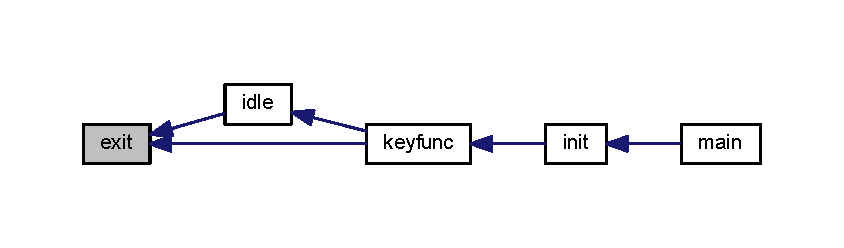
\includegraphics[width=350pt]{glut_8h_a6f255d924f7a6bb2c4be0c8c2f2d9ce3_icgraph}
\end{center}
\end{figure}


\index{glut.\+h@{glut.\+h}!glut\+Add\+Menu\+Entry@{glut\+Add\+Menu\+Entry}}
\index{glut\+Add\+Menu\+Entry@{glut\+Add\+Menu\+Entry}!glut.\+h@{glut.\+h}}
\subsubsection[{\texorpdfstring{glut\+Add\+Menu\+Entry(const char $\ast$label, int value)}{glutAddMenuEntry(const char *label, int value)}}]{\setlength{\rightskip}{0pt plus 5cm}{\bf G\+L\+U\+T\+A\+PI} void {\bf A\+P\+I\+E\+N\+T\+RY} glut\+Add\+Menu\+Entry (
\begin{DoxyParamCaption}
\item[{const char $\ast$}]{label, }
\item[{int}]{value}
\end{DoxyParamCaption}
)}\hypertarget{glut_8h_ad879b9b853c58e76b1a58c7b35eea7d9}{}\label{glut_8h_ad879b9b853c58e76b1a58c7b35eea7d9}
\index{glut.\+h@{glut.\+h}!glut\+Add\+Sub\+Menu@{glut\+Add\+Sub\+Menu}}
\index{glut\+Add\+Sub\+Menu@{glut\+Add\+Sub\+Menu}!glut.\+h@{glut.\+h}}
\subsubsection[{\texorpdfstring{glut\+Add\+Sub\+Menu(const char $\ast$label, int submenu)}{glutAddSubMenu(const char *label, int submenu)}}]{\setlength{\rightskip}{0pt plus 5cm}{\bf G\+L\+U\+T\+A\+PI} void {\bf A\+P\+I\+E\+N\+T\+RY} glut\+Add\+Sub\+Menu (
\begin{DoxyParamCaption}
\item[{const char $\ast$}]{label, }
\item[{int}]{submenu}
\end{DoxyParamCaption}
)}\hypertarget{glut_8h_a9556f1a5276612adef4ca7a883ce7bd7}{}\label{glut_8h_a9556f1a5276612adef4ca7a883ce7bd7}
\index{glut.\+h@{glut.\+h}!glut\+Attach\+Menu@{glut\+Attach\+Menu}}
\index{glut\+Attach\+Menu@{glut\+Attach\+Menu}!glut.\+h@{glut.\+h}}
\subsubsection[{\texorpdfstring{glut\+Attach\+Menu(int button)}{glutAttachMenu(int button)}}]{\setlength{\rightskip}{0pt plus 5cm}{\bf G\+L\+U\+T\+A\+PI} void {\bf A\+P\+I\+E\+N\+T\+RY} glut\+Attach\+Menu (
\begin{DoxyParamCaption}
\item[{int}]{button}
\end{DoxyParamCaption}
)}\hypertarget{glut_8h_ad5b169c2158dfe62d7d8112ab92d22e7}{}\label{glut_8h_ad5b169c2158dfe62d7d8112ab92d22e7}
\index{glut.\+h@{glut.\+h}!glut\+Bitmap\+Character@{glut\+Bitmap\+Character}}
\index{glut\+Bitmap\+Character@{glut\+Bitmap\+Character}!glut.\+h@{glut.\+h}}
\subsubsection[{\texorpdfstring{glut\+Bitmap\+Character(void $\ast$font, int character)}{glutBitmapCharacter(void *font, int character)}}]{\setlength{\rightskip}{0pt plus 5cm}{\bf G\+L\+U\+T\+A\+PI} void {\bf A\+P\+I\+E\+N\+T\+RY} glut\+Bitmap\+Character (
\begin{DoxyParamCaption}
\item[{void $\ast$}]{font, }
\item[{int}]{character}
\end{DoxyParamCaption}
)}\hypertarget{glut_8h_a014d6c29378b2b5c7063ff5bcd7252e6}{}\label{glut_8h_a014d6c29378b2b5c7063ff5bcd7252e6}
\index{glut.\+h@{glut.\+h}!glut\+Bitmap\+Length@{glut\+Bitmap\+Length}}
\index{glut\+Bitmap\+Length@{glut\+Bitmap\+Length}!glut.\+h@{glut.\+h}}
\subsubsection[{\texorpdfstring{glut\+Bitmap\+Length(void $\ast$font, const unsigned char $\ast$string)}{glutBitmapLength(void *font, const unsigned char *string)}}]{\setlength{\rightskip}{0pt plus 5cm}{\bf G\+L\+U\+T\+A\+PI} int {\bf A\+P\+I\+E\+N\+T\+RY} glut\+Bitmap\+Length (
\begin{DoxyParamCaption}
\item[{void $\ast$}]{font, }
\item[{const unsigned char $\ast$}]{string}
\end{DoxyParamCaption}
)}\hypertarget{glut_8h_aeadb419eaa7a1513f6296c2f29b461fa}{}\label{glut_8h_aeadb419eaa7a1513f6296c2f29b461fa}
\index{glut.\+h@{glut.\+h}!glut\+Bitmap\+Width@{glut\+Bitmap\+Width}}
\index{glut\+Bitmap\+Width@{glut\+Bitmap\+Width}!glut.\+h@{glut.\+h}}
\subsubsection[{\texorpdfstring{glut\+Bitmap\+Width(void $\ast$font, int character)}{glutBitmapWidth(void *font, int character)}}]{\setlength{\rightskip}{0pt plus 5cm}{\bf G\+L\+U\+T\+A\+PI} int {\bf A\+P\+I\+E\+N\+T\+RY} glut\+Bitmap\+Width (
\begin{DoxyParamCaption}
\item[{void $\ast$}]{font, }
\item[{int}]{character}
\end{DoxyParamCaption}
)}\hypertarget{glut_8h_a4b9eee6f4d8b2a1134ce32b6612a872a}{}\label{glut_8h_a4b9eee6f4d8b2a1134ce32b6612a872a}
\index{glut.\+h@{glut.\+h}!glut\+Button\+Box\+Func@{glut\+Button\+Box\+Func}}
\index{glut\+Button\+Box\+Func@{glut\+Button\+Box\+Func}!glut.\+h@{glut.\+h}}
\subsubsection[{\texorpdfstring{glut\+Button\+Box\+Func(void(\+G\+L\+U\+T\+C\+A\+L\+L\+B\+A\+C\+K $\ast$func)(int button, int state))}{glutButtonBoxFunc(void(GLUTCALLBACK *func)(int button, int state))}}]{\setlength{\rightskip}{0pt plus 5cm}{\bf G\+L\+U\+T\+A\+PI} void {\bf A\+P\+I\+E\+N\+T\+RY} glut\+Button\+Box\+Func (
\begin{DoxyParamCaption}
\item[{void({\bf G\+L\+U\+T\+C\+A\+L\+L\+B\+A\+CK} $\ast$func)(int button, int state)}]{}
\end{DoxyParamCaption}
)}\hypertarget{glut_8h_a740459d23af262295e71e0fefddae9e2}{}\label{glut_8h_a740459d23af262295e71e0fefddae9e2}
\index{glut.\+h@{glut.\+h}!glut\+Change\+To\+Menu\+Entry@{glut\+Change\+To\+Menu\+Entry}}
\index{glut\+Change\+To\+Menu\+Entry@{glut\+Change\+To\+Menu\+Entry}!glut.\+h@{glut.\+h}}
\subsubsection[{\texorpdfstring{glut\+Change\+To\+Menu\+Entry(int item, const char $\ast$label, int value)}{glutChangeToMenuEntry(int item, const char *label, int value)}}]{\setlength{\rightskip}{0pt plus 5cm}{\bf G\+L\+U\+T\+A\+PI} void {\bf A\+P\+I\+E\+N\+T\+RY} glut\+Change\+To\+Menu\+Entry (
\begin{DoxyParamCaption}
\item[{int}]{item, }
\item[{const char $\ast$}]{label, }
\item[{int}]{value}
\end{DoxyParamCaption}
)}\hypertarget{glut_8h_a80fcca98dfa0922e456aefbf5c35ff5f}{}\label{glut_8h_a80fcca98dfa0922e456aefbf5c35ff5f}
\index{glut.\+h@{glut.\+h}!glut\+Change\+To\+Sub\+Menu@{glut\+Change\+To\+Sub\+Menu}}
\index{glut\+Change\+To\+Sub\+Menu@{glut\+Change\+To\+Sub\+Menu}!glut.\+h@{glut.\+h}}
\subsubsection[{\texorpdfstring{glut\+Change\+To\+Sub\+Menu(int item, const char $\ast$label, int submenu)}{glutChangeToSubMenu(int item, const char *label, int submenu)}}]{\setlength{\rightskip}{0pt plus 5cm}{\bf G\+L\+U\+T\+A\+PI} void {\bf A\+P\+I\+E\+N\+T\+RY} glut\+Change\+To\+Sub\+Menu (
\begin{DoxyParamCaption}
\item[{int}]{item, }
\item[{const char $\ast$}]{label, }
\item[{int}]{submenu}
\end{DoxyParamCaption}
)}\hypertarget{glut_8h_a810444cc98d47a4b49460bcda65793d3}{}\label{glut_8h_a810444cc98d47a4b49460bcda65793d3}
\index{glut.\+h@{glut.\+h}!glut\+Copy\+Colormap@{glut\+Copy\+Colormap}}
\index{glut\+Copy\+Colormap@{glut\+Copy\+Colormap}!glut.\+h@{glut.\+h}}
\subsubsection[{\texorpdfstring{glut\+Copy\+Colormap(int win)}{glutCopyColormap(int win)}}]{\setlength{\rightskip}{0pt plus 5cm}{\bf G\+L\+U\+T\+A\+PI} void {\bf A\+P\+I\+E\+N\+T\+RY} glut\+Copy\+Colormap (
\begin{DoxyParamCaption}
\item[{int}]{win}
\end{DoxyParamCaption}
)}\hypertarget{glut_8h_a5976cfe11e724b6f4491e7755035aae7}{}\label{glut_8h_a5976cfe11e724b6f4491e7755035aae7}
\index{glut.\+h@{glut.\+h}!glut\+Create\+Menu@{glut\+Create\+Menu}}
\index{glut\+Create\+Menu@{glut\+Create\+Menu}!glut.\+h@{glut.\+h}}
\subsubsection[{\texorpdfstring{glut\+Create\+Menu(void(\+G\+L\+U\+T\+C\+A\+L\+L\+B\+A\+C\+K $\ast$func)(int))}{glutCreateMenu(void(GLUTCALLBACK *func)(int))}}]{\setlength{\rightskip}{0pt plus 5cm}{\bf G\+L\+U\+T\+A\+PI} int {\bf A\+P\+I\+E\+N\+T\+RY} glut\+Create\+Menu (
\begin{DoxyParamCaption}
\item[{void({\bf G\+L\+U\+T\+C\+A\+L\+L\+B\+A\+CK} $\ast$func)(int)}]{}
\end{DoxyParamCaption}
)}\hypertarget{glut_8h_a3a359b0601f11d3ccf58f6804a691168}{}\label{glut_8h_a3a359b0601f11d3ccf58f6804a691168}
\index{glut.\+h@{glut.\+h}!glut\+Create\+Sub\+Window@{glut\+Create\+Sub\+Window}}
\index{glut\+Create\+Sub\+Window@{glut\+Create\+Sub\+Window}!glut.\+h@{glut.\+h}}
\subsubsection[{\texorpdfstring{glut\+Create\+Sub\+Window(int win, int x, int y, int width, int height)}{glutCreateSubWindow(int win, int x, int y, int width, int height)}}]{\setlength{\rightskip}{0pt plus 5cm}{\bf G\+L\+U\+T\+A\+PI} int {\bf A\+P\+I\+E\+N\+T\+RY} glut\+Create\+Sub\+Window (
\begin{DoxyParamCaption}
\item[{int}]{win, }
\item[{int}]{x, }
\item[{int}]{y, }
\item[{int}]{width, }
\item[{int}]{height}
\end{DoxyParamCaption}
)}\hypertarget{glut_8h_ad13a95066ec52d117aca24555c8e2ba9}{}\label{glut_8h_ad13a95066ec52d117aca24555c8e2ba9}
\index{glut.\+h@{glut.\+h}!glut\+Create\+Window@{glut\+Create\+Window}}
\index{glut\+Create\+Window@{glut\+Create\+Window}!glut.\+h@{glut.\+h}}
\subsubsection[{\texorpdfstring{glut\+Create\+Window(const char $\ast$title)}{glutCreateWindow(const char *title)}}]{\setlength{\rightskip}{0pt plus 5cm}{\bf G\+L\+U\+T\+A\+PI} int {\bf A\+P\+I\+E\+N\+T\+RY} glut\+Create\+Window (
\begin{DoxyParamCaption}
\item[{const char $\ast$}]{title}
\end{DoxyParamCaption}
)}\hypertarget{glut_8h_aeb55aa096bb7a2f81779b924b5eac215}{}\label{glut_8h_aeb55aa096bb7a2f81779b924b5eac215}
\index{glut.\+h@{glut.\+h}!glut\+Destroy\+Menu@{glut\+Destroy\+Menu}}
\index{glut\+Destroy\+Menu@{glut\+Destroy\+Menu}!glut.\+h@{glut.\+h}}
\subsubsection[{\texorpdfstring{glut\+Destroy\+Menu(int menu)}{glutDestroyMenu(int menu)}}]{\setlength{\rightskip}{0pt plus 5cm}{\bf G\+L\+U\+T\+A\+PI} void {\bf A\+P\+I\+E\+N\+T\+RY} glut\+Destroy\+Menu (
\begin{DoxyParamCaption}
\item[{int}]{menu}
\end{DoxyParamCaption}
)}\hypertarget{glut_8h_ad5555a0c69eb306fe6651f9ccab96731}{}\label{glut_8h_ad5555a0c69eb306fe6651f9ccab96731}
\index{glut.\+h@{glut.\+h}!glut\+Destroy\+Window@{glut\+Destroy\+Window}}
\index{glut\+Destroy\+Window@{glut\+Destroy\+Window}!glut.\+h@{glut.\+h}}
\subsubsection[{\texorpdfstring{glut\+Destroy\+Window(int win)}{glutDestroyWindow(int win)}}]{\setlength{\rightskip}{0pt plus 5cm}{\bf G\+L\+U\+T\+A\+PI} void {\bf A\+P\+I\+E\+N\+T\+RY} glut\+Destroy\+Window (
\begin{DoxyParamCaption}
\item[{int}]{win}
\end{DoxyParamCaption}
)}\hypertarget{glut_8h_a6b081fbdac8ae609c1883075d7f6bf82}{}\label{glut_8h_a6b081fbdac8ae609c1883075d7f6bf82}
\index{glut.\+h@{glut.\+h}!glut\+Detach\+Menu@{glut\+Detach\+Menu}}
\index{glut\+Detach\+Menu@{glut\+Detach\+Menu}!glut.\+h@{glut.\+h}}
\subsubsection[{\texorpdfstring{glut\+Detach\+Menu(int button)}{glutDetachMenu(int button)}}]{\setlength{\rightskip}{0pt plus 5cm}{\bf G\+L\+U\+T\+A\+PI} void {\bf A\+P\+I\+E\+N\+T\+RY} glut\+Detach\+Menu (
\begin{DoxyParamCaption}
\item[{int}]{button}
\end{DoxyParamCaption}
)}\hypertarget{glut_8h_a7342114cf710e8953898f2ad5eb61f35}{}\label{glut_8h_a7342114cf710e8953898f2ad5eb61f35}
\index{glut.\+h@{glut.\+h}!glut\+Device\+Get@{glut\+Device\+Get}}
\index{glut\+Device\+Get@{glut\+Device\+Get}!glut.\+h@{glut.\+h}}
\subsubsection[{\texorpdfstring{glut\+Device\+Get(\+G\+Lenum type)}{glutDeviceGet(GLenum type)}}]{\setlength{\rightskip}{0pt plus 5cm}{\bf G\+L\+U\+T\+A\+PI} int {\bf A\+P\+I\+E\+N\+T\+RY} glut\+Device\+Get (
\begin{DoxyParamCaption}
\item[{G\+Lenum}]{type}
\end{DoxyParamCaption}
)}\hypertarget{glut_8h_acec09f2f73f7c9ebf0b8de6e84ad8089}{}\label{glut_8h_acec09f2f73f7c9ebf0b8de6e84ad8089}
\index{glut.\+h@{glut.\+h}!glut\+Dials\+Func@{glut\+Dials\+Func}}
\index{glut\+Dials\+Func@{glut\+Dials\+Func}!glut.\+h@{glut.\+h}}
\subsubsection[{\texorpdfstring{glut\+Dials\+Func(void(\+G\+L\+U\+T\+C\+A\+L\+L\+B\+A\+C\+K $\ast$func)(int dial, int value))}{glutDialsFunc(void(GLUTCALLBACK *func)(int dial, int value))}}]{\setlength{\rightskip}{0pt plus 5cm}{\bf G\+L\+U\+T\+A\+PI} void {\bf A\+P\+I\+E\+N\+T\+RY} glut\+Dials\+Func (
\begin{DoxyParamCaption}
\item[{void({\bf G\+L\+U\+T\+C\+A\+L\+L\+B\+A\+CK} $\ast$func)(int dial, int value)}]{}
\end{DoxyParamCaption}
)}\hypertarget{glut_8h_a0ec70b5e34818d6ed6c95bb085661bce}{}\label{glut_8h_a0ec70b5e34818d6ed6c95bb085661bce}
\index{glut.\+h@{glut.\+h}!glut\+Display\+Func@{glut\+Display\+Func}}
\index{glut\+Display\+Func@{glut\+Display\+Func}!glut.\+h@{glut.\+h}}
\subsubsection[{\texorpdfstring{glut\+Display\+Func(void(\+G\+L\+U\+T\+C\+A\+L\+L\+B\+A\+C\+K $\ast$func)(void))}{glutDisplayFunc(void(GLUTCALLBACK *func)(void))}}]{\setlength{\rightskip}{0pt plus 5cm}{\bf G\+L\+U\+T\+A\+PI} void {\bf A\+P\+I\+E\+N\+T\+RY} glut\+Display\+Func (
\begin{DoxyParamCaption}
\item[{void({\bf G\+L\+U\+T\+C\+A\+L\+L\+B\+A\+CK} $\ast$func)(void)}]{}
\end{DoxyParamCaption}
)}\hypertarget{glut_8h_a03cb35d5ea9264067a4cf08be8973f4f}{}\label{glut_8h_a03cb35d5ea9264067a4cf08be8973f4f}
\index{glut.\+h@{glut.\+h}!glut\+Enter\+Game\+Mode@{glut\+Enter\+Game\+Mode}}
\index{glut\+Enter\+Game\+Mode@{glut\+Enter\+Game\+Mode}!glut.\+h@{glut.\+h}}
\subsubsection[{\texorpdfstring{glut\+Enter\+Game\+Mode(void)}{glutEnterGameMode(void)}}]{\setlength{\rightskip}{0pt plus 5cm}{\bf G\+L\+U\+T\+A\+PI} int {\bf A\+P\+I\+E\+N\+T\+RY} glut\+Enter\+Game\+Mode (
\begin{DoxyParamCaption}
\item[{void}]{}
\end{DoxyParamCaption}
)}\hypertarget{glut_8h_a198d7f54b0086e9ea69c43826103089b}{}\label{glut_8h_a198d7f54b0086e9ea69c43826103089b}
\index{glut.\+h@{glut.\+h}!glut\+Entry\+Func@{glut\+Entry\+Func}}
\index{glut\+Entry\+Func@{glut\+Entry\+Func}!glut.\+h@{glut.\+h}}
\subsubsection[{\texorpdfstring{glut\+Entry\+Func(void(\+G\+L\+U\+T\+C\+A\+L\+L\+B\+A\+C\+K $\ast$func)(int state))}{glutEntryFunc(void(GLUTCALLBACK *func)(int state))}}]{\setlength{\rightskip}{0pt plus 5cm}{\bf G\+L\+U\+T\+A\+PI} void {\bf A\+P\+I\+E\+N\+T\+RY} glut\+Entry\+Func (
\begin{DoxyParamCaption}
\item[{void({\bf G\+L\+U\+T\+C\+A\+L\+L\+B\+A\+CK} $\ast$func)(int state)}]{}
\end{DoxyParamCaption}
)}\hypertarget{glut_8h_a231ef65d63503ca71a27bec67cbf806d}{}\label{glut_8h_a231ef65d63503ca71a27bec67cbf806d}
\index{glut.\+h@{glut.\+h}!glut\+Establish\+Overlay@{glut\+Establish\+Overlay}}
\index{glut\+Establish\+Overlay@{glut\+Establish\+Overlay}!glut.\+h@{glut.\+h}}
\subsubsection[{\texorpdfstring{glut\+Establish\+Overlay(void)}{glutEstablishOverlay(void)}}]{\setlength{\rightskip}{0pt plus 5cm}{\bf G\+L\+U\+T\+A\+PI} void {\bf A\+P\+I\+E\+N\+T\+RY} glut\+Establish\+Overlay (
\begin{DoxyParamCaption}
\item[{void}]{}
\end{DoxyParamCaption}
)}\hypertarget{glut_8h_ab1debf8002b8b6685a91368be3a7fdfd}{}\label{glut_8h_ab1debf8002b8b6685a91368be3a7fdfd}
\index{glut.\+h@{glut.\+h}!glut\+Extension\+Supported@{glut\+Extension\+Supported}}
\index{glut\+Extension\+Supported@{glut\+Extension\+Supported}!glut.\+h@{glut.\+h}}
\subsubsection[{\texorpdfstring{glut\+Extension\+Supported(const char $\ast$name)}{glutExtensionSupported(const char *name)}}]{\setlength{\rightskip}{0pt plus 5cm}{\bf G\+L\+U\+T\+A\+PI} int {\bf A\+P\+I\+E\+N\+T\+RY} glut\+Extension\+Supported (
\begin{DoxyParamCaption}
\item[{const char $\ast$}]{name}
\end{DoxyParamCaption}
)}\hypertarget{glut_8h_ac74f1efbf5aefc746c2ce0b64c8ede9c}{}\label{glut_8h_ac74f1efbf5aefc746c2ce0b64c8ede9c}
\index{glut.\+h@{glut.\+h}!glut\+Force\+Joystick\+Func@{glut\+Force\+Joystick\+Func}}
\index{glut\+Force\+Joystick\+Func@{glut\+Force\+Joystick\+Func}!glut.\+h@{glut.\+h}}
\subsubsection[{\texorpdfstring{glut\+Force\+Joystick\+Func(void)}{glutForceJoystickFunc(void)}}]{\setlength{\rightskip}{0pt plus 5cm}{\bf G\+L\+U\+T\+A\+PI} void {\bf A\+P\+I\+E\+N\+T\+RY} glut\+Force\+Joystick\+Func (
\begin{DoxyParamCaption}
\item[{void}]{}
\end{DoxyParamCaption}
)}\hypertarget{glut_8h_a544ce7e70b3470eccf53cf16a7154856}{}\label{glut_8h_a544ce7e70b3470eccf53cf16a7154856}
\index{glut.\+h@{glut.\+h}!glut\+Full\+Screen@{glut\+Full\+Screen}}
\index{glut\+Full\+Screen@{glut\+Full\+Screen}!glut.\+h@{glut.\+h}}
\subsubsection[{\texorpdfstring{glut\+Full\+Screen(void)}{glutFullScreen(void)}}]{\setlength{\rightskip}{0pt plus 5cm}{\bf G\+L\+U\+T\+A\+PI} void {\bf A\+P\+I\+E\+N\+T\+RY} glut\+Full\+Screen (
\begin{DoxyParamCaption}
\item[{void}]{}
\end{DoxyParamCaption}
)}\hypertarget{glut_8h_a825ff1ec0f9324d7ef57ff1b48b36209}{}\label{glut_8h_a825ff1ec0f9324d7ef57ff1b48b36209}
\index{glut.\+h@{glut.\+h}!glut\+Game\+Mode\+Get@{glut\+Game\+Mode\+Get}}
\index{glut\+Game\+Mode\+Get@{glut\+Game\+Mode\+Get}!glut.\+h@{glut.\+h}}
\subsubsection[{\texorpdfstring{glut\+Game\+Mode\+Get(\+G\+Lenum mode)}{glutGameModeGet(GLenum mode)}}]{\setlength{\rightskip}{0pt plus 5cm}{\bf G\+L\+U\+T\+A\+PI} int {\bf A\+P\+I\+E\+N\+T\+RY} glut\+Game\+Mode\+Get (
\begin{DoxyParamCaption}
\item[{G\+Lenum}]{mode}
\end{DoxyParamCaption}
)}\hypertarget{glut_8h_a637cfc18087be547ca581d26dd8ab2d2}{}\label{glut_8h_a637cfc18087be547ca581d26dd8ab2d2}
\index{glut.\+h@{glut.\+h}!glut\+Game\+Mode\+String@{glut\+Game\+Mode\+String}}
\index{glut\+Game\+Mode\+String@{glut\+Game\+Mode\+String}!glut.\+h@{glut.\+h}}
\subsubsection[{\texorpdfstring{glut\+Game\+Mode\+String(const char $\ast$string)}{glutGameModeString(const char *string)}}]{\setlength{\rightskip}{0pt plus 5cm}{\bf G\+L\+U\+T\+A\+PI} void {\bf A\+P\+I\+E\+N\+T\+RY} glut\+Game\+Mode\+String (
\begin{DoxyParamCaption}
\item[{const char $\ast$}]{string}
\end{DoxyParamCaption}
)}\hypertarget{glut_8h_ae4aa9aaaf290ae03767e6dfd3434abc5}{}\label{glut_8h_ae4aa9aaaf290ae03767e6dfd3434abc5}
\index{glut.\+h@{glut.\+h}!glut\+Get@{glut\+Get}}
\index{glut\+Get@{glut\+Get}!glut.\+h@{glut.\+h}}
\subsubsection[{\texorpdfstring{glut\+Get(\+G\+Lenum type)}{glutGet(GLenum type)}}]{\setlength{\rightskip}{0pt plus 5cm}{\bf G\+L\+U\+T\+A\+PI} int {\bf A\+P\+I\+E\+N\+T\+RY} glut\+Get (
\begin{DoxyParamCaption}
\item[{G\+Lenum}]{type}
\end{DoxyParamCaption}
)}\hypertarget{glut_8h_a1dbcb6b634a9c7c63672aca9bdae4ee9}{}\label{glut_8h_a1dbcb6b634a9c7c63672aca9bdae4ee9}
\index{glut.\+h@{glut.\+h}!glut\+Get\+Color@{glut\+Get\+Color}}
\index{glut\+Get\+Color@{glut\+Get\+Color}!glut.\+h@{glut.\+h}}
\subsubsection[{\texorpdfstring{glut\+Get\+Color(int ndx, int component)}{glutGetColor(int ndx, int component)}}]{\setlength{\rightskip}{0pt plus 5cm}{\bf G\+L\+U\+T\+A\+PI} G\+Lfloat {\bf A\+P\+I\+E\+N\+T\+RY} glut\+Get\+Color (
\begin{DoxyParamCaption}
\item[{int}]{ndx, }
\item[{int}]{component}
\end{DoxyParamCaption}
)}\hypertarget{glut_8h_a8ddf598d6a6d8d935997202472c28949}{}\label{glut_8h_a8ddf598d6a6d8d935997202472c28949}
\index{glut.\+h@{glut.\+h}!glut\+Get\+Menu@{glut\+Get\+Menu}}
\index{glut\+Get\+Menu@{glut\+Get\+Menu}!glut.\+h@{glut.\+h}}
\subsubsection[{\texorpdfstring{glut\+Get\+Menu(void)}{glutGetMenu(void)}}]{\setlength{\rightskip}{0pt plus 5cm}{\bf G\+L\+U\+T\+A\+PI} int {\bf A\+P\+I\+E\+N\+T\+RY} glut\+Get\+Menu (
\begin{DoxyParamCaption}
\item[{void}]{}
\end{DoxyParamCaption}
)}\hypertarget{glut_8h_abba12063a4f153b32998533b75a505c9}{}\label{glut_8h_abba12063a4f153b32998533b75a505c9}
\index{glut.\+h@{glut.\+h}!glut\+Get\+Modifiers@{glut\+Get\+Modifiers}}
\index{glut\+Get\+Modifiers@{glut\+Get\+Modifiers}!glut.\+h@{glut.\+h}}
\subsubsection[{\texorpdfstring{glut\+Get\+Modifiers(void)}{glutGetModifiers(void)}}]{\setlength{\rightskip}{0pt plus 5cm}{\bf G\+L\+U\+T\+A\+PI} int {\bf A\+P\+I\+E\+N\+T\+RY} glut\+Get\+Modifiers (
\begin{DoxyParamCaption}
\item[{void}]{}
\end{DoxyParamCaption}
)}\hypertarget{glut_8h_aa1ca712cb006916ba712fccfdda84dc4}{}\label{glut_8h_aa1ca712cb006916ba712fccfdda84dc4}
\index{glut.\+h@{glut.\+h}!glut\+Get\+Window@{glut\+Get\+Window}}
\index{glut\+Get\+Window@{glut\+Get\+Window}!glut.\+h@{glut.\+h}}
\subsubsection[{\texorpdfstring{glut\+Get\+Window(void)}{glutGetWindow(void)}}]{\setlength{\rightskip}{0pt plus 5cm}{\bf G\+L\+U\+T\+A\+PI} int {\bf A\+P\+I\+E\+N\+T\+RY} glut\+Get\+Window (
\begin{DoxyParamCaption}
\item[{void}]{}
\end{DoxyParamCaption}
)}\hypertarget{glut_8h_a660d1612b47f2d0ea5795ae253b18c14}{}\label{glut_8h_a660d1612b47f2d0ea5795ae253b18c14}
\index{glut.\+h@{glut.\+h}!glut\+Hide\+Overlay@{glut\+Hide\+Overlay}}
\index{glut\+Hide\+Overlay@{glut\+Hide\+Overlay}!glut.\+h@{glut.\+h}}
\subsubsection[{\texorpdfstring{glut\+Hide\+Overlay(void)}{glutHideOverlay(void)}}]{\setlength{\rightskip}{0pt plus 5cm}{\bf G\+L\+U\+T\+A\+PI} void {\bf A\+P\+I\+E\+N\+T\+RY} glut\+Hide\+Overlay (
\begin{DoxyParamCaption}
\item[{void}]{}
\end{DoxyParamCaption}
)}\hypertarget{glut_8h_ade82bbf847ef99417224806532d15a2c}{}\label{glut_8h_ade82bbf847ef99417224806532d15a2c}
\index{glut.\+h@{glut.\+h}!glut\+Hide\+Window@{glut\+Hide\+Window}}
\index{glut\+Hide\+Window@{glut\+Hide\+Window}!glut.\+h@{glut.\+h}}
\subsubsection[{\texorpdfstring{glut\+Hide\+Window(void)}{glutHideWindow(void)}}]{\setlength{\rightskip}{0pt plus 5cm}{\bf G\+L\+U\+T\+A\+PI} void {\bf A\+P\+I\+E\+N\+T\+RY} glut\+Hide\+Window (
\begin{DoxyParamCaption}
\item[{void}]{}
\end{DoxyParamCaption}
)}\hypertarget{glut_8h_a6b64edd75bc235bde37462e1477cc3bd}{}\label{glut_8h_a6b64edd75bc235bde37462e1477cc3bd}
\index{glut.\+h@{glut.\+h}!glut\+Iconify\+Window@{glut\+Iconify\+Window}}
\index{glut\+Iconify\+Window@{glut\+Iconify\+Window}!glut.\+h@{glut.\+h}}
\subsubsection[{\texorpdfstring{glut\+Iconify\+Window(void)}{glutIconifyWindow(void)}}]{\setlength{\rightskip}{0pt plus 5cm}{\bf G\+L\+U\+T\+A\+PI} void {\bf A\+P\+I\+E\+N\+T\+RY} glut\+Iconify\+Window (
\begin{DoxyParamCaption}
\item[{void}]{}
\end{DoxyParamCaption}
)}\hypertarget{glut_8h_a6e7e9f1e877fd7a291108479a34374cd}{}\label{glut_8h_a6e7e9f1e877fd7a291108479a34374cd}
\index{glut.\+h@{glut.\+h}!glut\+Idle\+Func@{glut\+Idle\+Func}}
\index{glut\+Idle\+Func@{glut\+Idle\+Func}!glut.\+h@{glut.\+h}}
\subsubsection[{\texorpdfstring{glut\+Idle\+Func(void(\+G\+L\+U\+T\+C\+A\+L\+L\+B\+A\+C\+K $\ast$func)(void))}{glutIdleFunc(void(GLUTCALLBACK *func)(void))}}]{\setlength{\rightskip}{0pt plus 5cm}{\bf G\+L\+U\+T\+A\+PI} void {\bf A\+P\+I\+E\+N\+T\+RY} glut\+Idle\+Func (
\begin{DoxyParamCaption}
\item[{void({\bf G\+L\+U\+T\+C\+A\+L\+L\+B\+A\+CK} $\ast$func)(void)}]{}
\end{DoxyParamCaption}
)}\hypertarget{glut_8h_a52b8f31c71db8649f8cf769b1f614e92}{}\label{glut_8h_a52b8f31c71db8649f8cf769b1f614e92}
\index{glut.\+h@{glut.\+h}!glut\+Ignore\+Key\+Repeat@{glut\+Ignore\+Key\+Repeat}}
\index{glut\+Ignore\+Key\+Repeat@{glut\+Ignore\+Key\+Repeat}!glut.\+h@{glut.\+h}}
\subsubsection[{\texorpdfstring{glut\+Ignore\+Key\+Repeat(int ignore)}{glutIgnoreKeyRepeat(int ignore)}}]{\setlength{\rightskip}{0pt plus 5cm}{\bf G\+L\+U\+T\+A\+PI} void {\bf A\+P\+I\+E\+N\+T\+RY} glut\+Ignore\+Key\+Repeat (
\begin{DoxyParamCaption}
\item[{int}]{ignore}
\end{DoxyParamCaption}
)}\hypertarget{glut_8h_a5e88e6cbd44974b50ad37b3f873aa0b7}{}\label{glut_8h_a5e88e6cbd44974b50ad37b3f873aa0b7}
\index{glut.\+h@{glut.\+h}!glut\+Init@{glut\+Init}}
\index{glut\+Init@{glut\+Init}!glut.\+h@{glut.\+h}}
\subsubsection[{\texorpdfstring{glut\+Init(int $\ast$argcp, char $\ast$$\ast$argv)}{glutInit(int *argcp, char **argv)}}]{\setlength{\rightskip}{0pt plus 5cm}{\bf G\+L\+U\+T\+A\+PI} void {\bf A\+P\+I\+E\+N\+T\+RY} glut\+Init (
\begin{DoxyParamCaption}
\item[{int $\ast$}]{argcp, }
\item[{char $\ast$$\ast$}]{argv}
\end{DoxyParamCaption}
)}\hypertarget{glut_8h_a2bed9db3feab26e4087ce7e710126438}{}\label{glut_8h_a2bed9db3feab26e4087ce7e710126438}
\index{glut.\+h@{glut.\+h}!glut\+Init\+Display\+Mode@{glut\+Init\+Display\+Mode}}
\index{glut\+Init\+Display\+Mode@{glut\+Init\+Display\+Mode}!glut.\+h@{glut.\+h}}
\subsubsection[{\texorpdfstring{glut\+Init\+Display\+Mode(unsigned int mode)}{glutInitDisplayMode(unsigned int mode)}}]{\setlength{\rightskip}{0pt plus 5cm}{\bf G\+L\+U\+T\+A\+PI} void {\bf A\+P\+I\+E\+N\+T\+RY} glut\+Init\+Display\+Mode (
\begin{DoxyParamCaption}
\item[{unsigned int}]{mode}
\end{DoxyParamCaption}
)}\hypertarget{glut_8h_a2b7096cd64af1c2372f5f3953635d2ed}{}\label{glut_8h_a2b7096cd64af1c2372f5f3953635d2ed}
\index{glut.\+h@{glut.\+h}!glut\+Init\+Display\+String@{glut\+Init\+Display\+String}}
\index{glut\+Init\+Display\+String@{glut\+Init\+Display\+String}!glut.\+h@{glut.\+h}}
\subsubsection[{\texorpdfstring{glut\+Init\+Display\+String(const char $\ast$string)}{glutInitDisplayString(const char *string)}}]{\setlength{\rightskip}{0pt plus 5cm}{\bf G\+L\+U\+T\+A\+PI} void {\bf A\+P\+I\+E\+N\+T\+RY} glut\+Init\+Display\+String (
\begin{DoxyParamCaption}
\item[{const char $\ast$}]{string}
\end{DoxyParamCaption}
)}\hypertarget{glut_8h_a3fbdf5362eae63e91a90ec854ea86d98}{}\label{glut_8h_a3fbdf5362eae63e91a90ec854ea86d98}
\index{glut.\+h@{glut.\+h}!glut\+Init\+Window\+Position@{glut\+Init\+Window\+Position}}
\index{glut\+Init\+Window\+Position@{glut\+Init\+Window\+Position}!glut.\+h@{glut.\+h}}
\subsubsection[{\texorpdfstring{glut\+Init\+Window\+Position(int x, int y)}{glutInitWindowPosition(int x, int y)}}]{\setlength{\rightskip}{0pt plus 5cm}{\bf G\+L\+U\+T\+A\+PI} void {\bf A\+P\+I\+E\+N\+T\+RY} glut\+Init\+Window\+Position (
\begin{DoxyParamCaption}
\item[{int}]{x, }
\item[{int}]{y}
\end{DoxyParamCaption}
)}\hypertarget{glut_8h_a76cc6cf86f45849b366ceea0f527680f}{}\label{glut_8h_a76cc6cf86f45849b366ceea0f527680f}
\index{glut.\+h@{glut.\+h}!glut\+Init\+Window\+Size@{glut\+Init\+Window\+Size}}
\index{glut\+Init\+Window\+Size@{glut\+Init\+Window\+Size}!glut.\+h@{glut.\+h}}
\subsubsection[{\texorpdfstring{glut\+Init\+Window\+Size(int width, int height)}{glutInitWindowSize(int width, int height)}}]{\setlength{\rightskip}{0pt plus 5cm}{\bf G\+L\+U\+T\+A\+PI} void {\bf A\+P\+I\+E\+N\+T\+RY} glut\+Init\+Window\+Size (
\begin{DoxyParamCaption}
\item[{int}]{width, }
\item[{int}]{height}
\end{DoxyParamCaption}
)}\hypertarget{glut_8h_a9501b45b128db8d666d197715b7adf06}{}\label{glut_8h_a9501b45b128db8d666d197715b7adf06}
\index{glut.\+h@{glut.\+h}!glut\+Joystick\+Func@{glut\+Joystick\+Func}}
\index{glut\+Joystick\+Func@{glut\+Joystick\+Func}!glut.\+h@{glut.\+h}}
\subsubsection[{\texorpdfstring{glut\+Joystick\+Func(void(\+G\+L\+U\+T\+C\+A\+L\+L\+B\+A\+C\+K $\ast$func)(unsigned int button\+Mask, int x, int y, int z), int poll\+Interval)}{glutJoystickFunc(void(GLUTCALLBACK *func)(unsigned int buttonMask, int x, int y, int z), int pollInterval)}}]{\setlength{\rightskip}{0pt plus 5cm}{\bf G\+L\+U\+T\+A\+PI} void {\bf A\+P\+I\+E\+N\+T\+RY} glut\+Joystick\+Func (
\begin{DoxyParamCaption}
\item[{void({\bf G\+L\+U\+T\+C\+A\+L\+L\+B\+A\+CK} $\ast$func)(unsigned int button\+Mask, int x, int y, int z)}]{, }
\item[{int}]{poll\+Interval}
\end{DoxyParamCaption}
)}\hypertarget{glut_8h_a464b1e4d6c4080eab11b446ca32c9e3a}{}\label{glut_8h_a464b1e4d6c4080eab11b446ca32c9e3a}
\index{glut.\+h@{glut.\+h}!glut\+Keyboard\+Func@{glut\+Keyboard\+Func}}
\index{glut\+Keyboard\+Func@{glut\+Keyboard\+Func}!glut.\+h@{glut.\+h}}
\subsubsection[{\texorpdfstring{glut\+Keyboard\+Func(void(\+G\+L\+U\+T\+C\+A\+L\+L\+B\+A\+C\+K $\ast$func)(unsigned char key, int x, int y))}{glutKeyboardFunc(void(GLUTCALLBACK *func)(unsigned char key, int x, int y))}}]{\setlength{\rightskip}{0pt plus 5cm}{\bf G\+L\+U\+T\+A\+PI} void {\bf A\+P\+I\+E\+N\+T\+RY} glut\+Keyboard\+Func (
\begin{DoxyParamCaption}
\item[{void({\bf G\+L\+U\+T\+C\+A\+L\+L\+B\+A\+CK} $\ast$func)(unsigned char key, int x, int y)}]{}
\end{DoxyParamCaption}
)}\hypertarget{glut_8h_a5098c4d36b149b8ad436786ed24b03a3}{}\label{glut_8h_a5098c4d36b149b8ad436786ed24b03a3}
\index{glut.\+h@{glut.\+h}!glut\+Keyboard\+Up\+Func@{glut\+Keyboard\+Up\+Func}}
\index{glut\+Keyboard\+Up\+Func@{glut\+Keyboard\+Up\+Func}!glut.\+h@{glut.\+h}}
\subsubsection[{\texorpdfstring{glut\+Keyboard\+Up\+Func(void(\+G\+L\+U\+T\+C\+A\+L\+L\+B\+A\+C\+K $\ast$func)(unsigned char key, int x, int y))}{glutKeyboardUpFunc(void(GLUTCALLBACK *func)(unsigned char key, int x, int y))}}]{\setlength{\rightskip}{0pt plus 5cm}{\bf G\+L\+U\+T\+A\+PI} void {\bf A\+P\+I\+E\+N\+T\+RY} glut\+Keyboard\+Up\+Func (
\begin{DoxyParamCaption}
\item[{void({\bf G\+L\+U\+T\+C\+A\+L\+L\+B\+A\+CK} $\ast$func)(unsigned char key, int x, int y)}]{}
\end{DoxyParamCaption}
)}\hypertarget{glut_8h_af2f5d3a7d9eae641db7b1e6410d8d0f8}{}\label{glut_8h_af2f5d3a7d9eae641db7b1e6410d8d0f8}
\index{glut.\+h@{glut.\+h}!glut\+Layer\+Get@{glut\+Layer\+Get}}
\index{glut\+Layer\+Get@{glut\+Layer\+Get}!glut.\+h@{glut.\+h}}
\subsubsection[{\texorpdfstring{glut\+Layer\+Get(\+G\+Lenum type)}{glutLayerGet(GLenum type)}}]{\setlength{\rightskip}{0pt plus 5cm}{\bf G\+L\+U\+T\+A\+PI} int {\bf A\+P\+I\+E\+N\+T\+RY} glut\+Layer\+Get (
\begin{DoxyParamCaption}
\item[{G\+Lenum}]{type}
\end{DoxyParamCaption}
)}\hypertarget{glut_8h_a840d862b7c2f7e5b46401591e1a9e5ee}{}\label{glut_8h_a840d862b7c2f7e5b46401591e1a9e5ee}
\index{glut.\+h@{glut.\+h}!glut\+Leave\+Game\+Mode@{glut\+Leave\+Game\+Mode}}
\index{glut\+Leave\+Game\+Mode@{glut\+Leave\+Game\+Mode}!glut.\+h@{glut.\+h}}
\subsubsection[{\texorpdfstring{glut\+Leave\+Game\+Mode(void)}{glutLeaveGameMode(void)}}]{\setlength{\rightskip}{0pt plus 5cm}{\bf G\+L\+U\+T\+A\+PI} void {\bf A\+P\+I\+E\+N\+T\+RY} glut\+Leave\+Game\+Mode (
\begin{DoxyParamCaption}
\item[{void}]{}
\end{DoxyParamCaption}
)}\hypertarget{glut_8h_afa9a345cb734837434150ec4892cfa42}{}\label{glut_8h_afa9a345cb734837434150ec4892cfa42}
\index{glut.\+h@{glut.\+h}!glut\+Main\+Loop@{glut\+Main\+Loop}}
\index{glut\+Main\+Loop@{glut\+Main\+Loop}!glut.\+h@{glut.\+h}}
\subsubsection[{\texorpdfstring{glut\+Main\+Loop(void)}{glutMainLoop(void)}}]{\setlength{\rightskip}{0pt plus 5cm}{\bf G\+L\+U\+T\+A\+PI} void {\bf A\+P\+I\+E\+N\+T\+RY} glut\+Main\+Loop (
\begin{DoxyParamCaption}
\item[{void}]{}
\end{DoxyParamCaption}
)}\hypertarget{glut_8h_a9dab481c63c132f43ad05a1e8c0b5a0f}{}\label{glut_8h_a9dab481c63c132f43ad05a1e8c0b5a0f}
\index{glut.\+h@{glut.\+h}!glut\+Menu\+State\+Func@{glut\+Menu\+State\+Func}}
\index{glut\+Menu\+State\+Func@{glut\+Menu\+State\+Func}!glut.\+h@{glut.\+h}}
\subsubsection[{\texorpdfstring{glut\+Menu\+State\+Func(void(\+G\+L\+U\+T\+C\+A\+L\+L\+B\+A\+C\+K $\ast$func)(int state))}{glutMenuStateFunc(void(GLUTCALLBACK *func)(int state))}}]{\setlength{\rightskip}{0pt plus 5cm}{\bf G\+L\+U\+T\+A\+PI} void {\bf A\+P\+I\+E\+N\+T\+RY} glut\+Menu\+State\+Func (
\begin{DoxyParamCaption}
\item[{void({\bf G\+L\+U\+T\+C\+A\+L\+L\+B\+A\+CK} $\ast$func)(int state)}]{}
\end{DoxyParamCaption}
)}\hypertarget{glut_8h_a6451be871a0da2c0bb0270d876f17902}{}\label{glut_8h_a6451be871a0da2c0bb0270d876f17902}
\index{glut.\+h@{glut.\+h}!glut\+Menu\+Status\+Func@{glut\+Menu\+Status\+Func}}
\index{glut\+Menu\+Status\+Func@{glut\+Menu\+Status\+Func}!glut.\+h@{glut.\+h}}
\subsubsection[{\texorpdfstring{glut\+Menu\+Status\+Func(void(\+G\+L\+U\+T\+C\+A\+L\+L\+B\+A\+C\+K $\ast$func)(int status, int x, int y))}{glutMenuStatusFunc(void(GLUTCALLBACK *func)(int status, int x, int y))}}]{\setlength{\rightskip}{0pt plus 5cm}{\bf G\+L\+U\+T\+A\+PI} void {\bf A\+P\+I\+E\+N\+T\+RY} glut\+Menu\+Status\+Func (
\begin{DoxyParamCaption}
\item[{void({\bf G\+L\+U\+T\+C\+A\+L\+L\+B\+A\+CK} $\ast$func)(int status, int x, int y)}]{}
\end{DoxyParamCaption}
)}\hypertarget{glut_8h_aadc16896d80701943636cb22495abcfc}{}\label{glut_8h_aadc16896d80701943636cb22495abcfc}
\index{glut.\+h@{glut.\+h}!glut\+Motion\+Func@{glut\+Motion\+Func}}
\index{glut\+Motion\+Func@{glut\+Motion\+Func}!glut.\+h@{glut.\+h}}
\subsubsection[{\texorpdfstring{glut\+Motion\+Func(void(\+G\+L\+U\+T\+C\+A\+L\+L\+B\+A\+C\+K $\ast$func)(int x, int y))}{glutMotionFunc(void(GLUTCALLBACK *func)(int x, int y))}}]{\setlength{\rightskip}{0pt plus 5cm}{\bf G\+L\+U\+T\+A\+PI} void {\bf A\+P\+I\+E\+N\+T\+RY} glut\+Motion\+Func (
\begin{DoxyParamCaption}
\item[{void({\bf G\+L\+U\+T\+C\+A\+L\+L\+B\+A\+CK} $\ast$func)(int x, int y)}]{}
\end{DoxyParamCaption}
)}\hypertarget{glut_8h_a437895d0cd962908790ba033cb01e0f4}{}\label{glut_8h_a437895d0cd962908790ba033cb01e0f4}
\index{glut.\+h@{glut.\+h}!glut\+Mouse\+Func@{glut\+Mouse\+Func}}
\index{glut\+Mouse\+Func@{glut\+Mouse\+Func}!glut.\+h@{glut.\+h}}
\subsubsection[{\texorpdfstring{glut\+Mouse\+Func(void(\+G\+L\+U\+T\+C\+A\+L\+L\+B\+A\+C\+K $\ast$func)(int button, int state, int x, int y))}{glutMouseFunc(void(GLUTCALLBACK *func)(int button, int state, int x, int y))}}]{\setlength{\rightskip}{0pt plus 5cm}{\bf G\+L\+U\+T\+A\+PI} void {\bf A\+P\+I\+E\+N\+T\+RY} glut\+Mouse\+Func (
\begin{DoxyParamCaption}
\item[{void({\bf G\+L\+U\+T\+C\+A\+L\+L\+B\+A\+CK} $\ast$func)(int button, int state, int x, int y)}]{}
\end{DoxyParamCaption}
)}\hypertarget{glut_8h_aea5873dafdddd04820a338d438f8497b}{}\label{glut_8h_aea5873dafdddd04820a338d438f8497b}
\index{glut.\+h@{glut.\+h}!glut\+Overlay\+Display\+Func@{glut\+Overlay\+Display\+Func}}
\index{glut\+Overlay\+Display\+Func@{glut\+Overlay\+Display\+Func}!glut.\+h@{glut.\+h}}
\subsubsection[{\texorpdfstring{glut\+Overlay\+Display\+Func(void(\+G\+L\+U\+T\+C\+A\+L\+L\+B\+A\+C\+K $\ast$func)(void))}{glutOverlayDisplayFunc(void(GLUTCALLBACK *func)(void))}}]{\setlength{\rightskip}{0pt plus 5cm}{\bf G\+L\+U\+T\+A\+PI} void {\bf A\+P\+I\+E\+N\+T\+RY} glut\+Overlay\+Display\+Func (
\begin{DoxyParamCaption}
\item[{void({\bf G\+L\+U\+T\+C\+A\+L\+L\+B\+A\+CK} $\ast$func)(void)}]{}
\end{DoxyParamCaption}
)}\hypertarget{glut_8h_a1727642ed452086ddb61d7eb8791a1e7}{}\label{glut_8h_a1727642ed452086ddb61d7eb8791a1e7}
\index{glut.\+h@{glut.\+h}!glut\+Passive\+Motion\+Func@{glut\+Passive\+Motion\+Func}}
\index{glut\+Passive\+Motion\+Func@{glut\+Passive\+Motion\+Func}!glut.\+h@{glut.\+h}}
\subsubsection[{\texorpdfstring{glut\+Passive\+Motion\+Func(void(\+G\+L\+U\+T\+C\+A\+L\+L\+B\+A\+C\+K $\ast$func)(int x, int y))}{glutPassiveMotionFunc(void(GLUTCALLBACK *func)(int x, int y))}}]{\setlength{\rightskip}{0pt plus 5cm}{\bf G\+L\+U\+T\+A\+PI} void {\bf A\+P\+I\+E\+N\+T\+RY} glut\+Passive\+Motion\+Func (
\begin{DoxyParamCaption}
\item[{void({\bf G\+L\+U\+T\+C\+A\+L\+L\+B\+A\+CK} $\ast$func)(int x, int y)}]{}
\end{DoxyParamCaption}
)}\hypertarget{glut_8h_a5dd0b0c28f116a6b217d56e844898207}{}\label{glut_8h_a5dd0b0c28f116a6b217d56e844898207}
\index{glut.\+h@{glut.\+h}!glut\+Pop\+Window@{glut\+Pop\+Window}}
\index{glut\+Pop\+Window@{glut\+Pop\+Window}!glut.\+h@{glut.\+h}}
\subsubsection[{\texorpdfstring{glut\+Pop\+Window(void)}{glutPopWindow(void)}}]{\setlength{\rightskip}{0pt plus 5cm}{\bf G\+L\+U\+T\+A\+PI} void {\bf A\+P\+I\+E\+N\+T\+RY} glut\+Pop\+Window (
\begin{DoxyParamCaption}
\item[{void}]{}
\end{DoxyParamCaption}
)}\hypertarget{glut_8h_ac324e575191ff76fea304b0ec0d92d37}{}\label{glut_8h_ac324e575191ff76fea304b0ec0d92d37}
\index{glut.\+h@{glut.\+h}!glut\+Position\+Window@{glut\+Position\+Window}}
\index{glut\+Position\+Window@{glut\+Position\+Window}!glut.\+h@{glut.\+h}}
\subsubsection[{\texorpdfstring{glut\+Position\+Window(int x, int y)}{glutPositionWindow(int x, int y)}}]{\setlength{\rightskip}{0pt plus 5cm}{\bf G\+L\+U\+T\+A\+PI} void {\bf A\+P\+I\+E\+N\+T\+RY} glut\+Position\+Window (
\begin{DoxyParamCaption}
\item[{int}]{x, }
\item[{int}]{y}
\end{DoxyParamCaption}
)}\hypertarget{glut_8h_addc944fd8637d7ff7c21d7633b89ba14}{}\label{glut_8h_addc944fd8637d7ff7c21d7633b89ba14}
\index{glut.\+h@{glut.\+h}!glut\+Post\+Overlay\+Redisplay@{glut\+Post\+Overlay\+Redisplay}}
\index{glut\+Post\+Overlay\+Redisplay@{glut\+Post\+Overlay\+Redisplay}!glut.\+h@{glut.\+h}}
\subsubsection[{\texorpdfstring{glut\+Post\+Overlay\+Redisplay(void)}{glutPostOverlayRedisplay(void)}}]{\setlength{\rightskip}{0pt plus 5cm}{\bf G\+L\+U\+T\+A\+PI} void {\bf A\+P\+I\+E\+N\+T\+RY} glut\+Post\+Overlay\+Redisplay (
\begin{DoxyParamCaption}
\item[{void}]{}
\end{DoxyParamCaption}
)}\hypertarget{glut_8h_afcfa0f563920deaa3632bf027b56dbd3}{}\label{glut_8h_afcfa0f563920deaa3632bf027b56dbd3}
\index{glut.\+h@{glut.\+h}!glut\+Post\+Redisplay@{glut\+Post\+Redisplay}}
\index{glut\+Post\+Redisplay@{glut\+Post\+Redisplay}!glut.\+h@{glut.\+h}}
\subsubsection[{\texorpdfstring{glut\+Post\+Redisplay(void)}{glutPostRedisplay(void)}}]{\setlength{\rightskip}{0pt plus 5cm}{\bf G\+L\+U\+T\+A\+PI} void {\bf A\+P\+I\+E\+N\+T\+RY} glut\+Post\+Redisplay (
\begin{DoxyParamCaption}
\item[{void}]{}
\end{DoxyParamCaption}
)}\hypertarget{glut_8h_a4844b2228c60161628d1cd3b52d93a47}{}\label{glut_8h_a4844b2228c60161628d1cd3b52d93a47}
\index{glut.\+h@{glut.\+h}!glut\+Post\+Window\+Overlay\+Redisplay@{glut\+Post\+Window\+Overlay\+Redisplay}}
\index{glut\+Post\+Window\+Overlay\+Redisplay@{glut\+Post\+Window\+Overlay\+Redisplay}!glut.\+h@{glut.\+h}}
\subsubsection[{\texorpdfstring{glut\+Post\+Window\+Overlay\+Redisplay(int win)}{glutPostWindowOverlayRedisplay(int win)}}]{\setlength{\rightskip}{0pt plus 5cm}{\bf G\+L\+U\+T\+A\+PI} void {\bf A\+P\+I\+E\+N\+T\+RY} glut\+Post\+Window\+Overlay\+Redisplay (
\begin{DoxyParamCaption}
\item[{int}]{win}
\end{DoxyParamCaption}
)}\hypertarget{glut_8h_a6ed8ca14ff36fd6fda379a89b8f7bf58}{}\label{glut_8h_a6ed8ca14ff36fd6fda379a89b8f7bf58}
\index{glut.\+h@{glut.\+h}!glut\+Post\+Window\+Redisplay@{glut\+Post\+Window\+Redisplay}}
\index{glut\+Post\+Window\+Redisplay@{glut\+Post\+Window\+Redisplay}!glut.\+h@{glut.\+h}}
\subsubsection[{\texorpdfstring{glut\+Post\+Window\+Redisplay(int win)}{glutPostWindowRedisplay(int win)}}]{\setlength{\rightskip}{0pt plus 5cm}{\bf G\+L\+U\+T\+A\+PI} void {\bf A\+P\+I\+E\+N\+T\+RY} glut\+Post\+Window\+Redisplay (
\begin{DoxyParamCaption}
\item[{int}]{win}
\end{DoxyParamCaption}
)}\hypertarget{glut_8h_aea39e494d75668057445d333b0b9a37c}{}\label{glut_8h_aea39e494d75668057445d333b0b9a37c}
\index{glut.\+h@{glut.\+h}!glut\+Push\+Window@{glut\+Push\+Window}}
\index{glut\+Push\+Window@{glut\+Push\+Window}!glut.\+h@{glut.\+h}}
\subsubsection[{\texorpdfstring{glut\+Push\+Window(void)}{glutPushWindow(void)}}]{\setlength{\rightskip}{0pt plus 5cm}{\bf G\+L\+U\+T\+A\+PI} void {\bf A\+P\+I\+E\+N\+T\+RY} glut\+Push\+Window (
\begin{DoxyParamCaption}
\item[{void}]{}
\end{DoxyParamCaption}
)}\hypertarget{glut_8h_ac449ad8fb577eb843dd20fb07b6e28cd}{}\label{glut_8h_ac449ad8fb577eb843dd20fb07b6e28cd}
\index{glut.\+h@{glut.\+h}!glut\+Remove\+Menu\+Item@{glut\+Remove\+Menu\+Item}}
\index{glut\+Remove\+Menu\+Item@{glut\+Remove\+Menu\+Item}!glut.\+h@{glut.\+h}}
\subsubsection[{\texorpdfstring{glut\+Remove\+Menu\+Item(int item)}{glutRemoveMenuItem(int item)}}]{\setlength{\rightskip}{0pt plus 5cm}{\bf G\+L\+U\+T\+A\+PI} void {\bf A\+P\+I\+E\+N\+T\+RY} glut\+Remove\+Menu\+Item (
\begin{DoxyParamCaption}
\item[{int}]{item}
\end{DoxyParamCaption}
)}\hypertarget{glut_8h_afea40e85451d30fad99af0c5f0094790}{}\label{glut_8h_afea40e85451d30fad99af0c5f0094790}
\index{glut.\+h@{glut.\+h}!glut\+Remove\+Overlay@{glut\+Remove\+Overlay}}
\index{glut\+Remove\+Overlay@{glut\+Remove\+Overlay}!glut.\+h@{glut.\+h}}
\subsubsection[{\texorpdfstring{glut\+Remove\+Overlay(void)}{glutRemoveOverlay(void)}}]{\setlength{\rightskip}{0pt plus 5cm}{\bf G\+L\+U\+T\+A\+PI} void {\bf A\+P\+I\+E\+N\+T\+RY} glut\+Remove\+Overlay (
\begin{DoxyParamCaption}
\item[{void}]{}
\end{DoxyParamCaption}
)}\hypertarget{glut_8h_a331dc63969f4ab3bbf9f32a3aa4c6e9a}{}\label{glut_8h_a331dc63969f4ab3bbf9f32a3aa4c6e9a}
\index{glut.\+h@{glut.\+h}!glut\+Report\+Errors@{glut\+Report\+Errors}}
\index{glut\+Report\+Errors@{glut\+Report\+Errors}!glut.\+h@{glut.\+h}}
\subsubsection[{\texorpdfstring{glut\+Report\+Errors(void)}{glutReportErrors(void)}}]{\setlength{\rightskip}{0pt plus 5cm}{\bf G\+L\+U\+T\+A\+PI} void {\bf A\+P\+I\+E\+N\+T\+RY} glut\+Report\+Errors (
\begin{DoxyParamCaption}
\item[{void}]{}
\end{DoxyParamCaption}
)}\hypertarget{glut_8h_a733ba6aaa5c7cfc7f66839d1cde32937}{}\label{glut_8h_a733ba6aaa5c7cfc7f66839d1cde32937}
\index{glut.\+h@{glut.\+h}!glut\+Reshape\+Func@{glut\+Reshape\+Func}}
\index{glut\+Reshape\+Func@{glut\+Reshape\+Func}!glut.\+h@{glut.\+h}}
\subsubsection[{\texorpdfstring{glut\+Reshape\+Func(void(\+G\+L\+U\+T\+C\+A\+L\+L\+B\+A\+C\+K $\ast$func)(int width, int height))}{glutReshapeFunc(void(GLUTCALLBACK *func)(int width, int height))}}]{\setlength{\rightskip}{0pt plus 5cm}{\bf G\+L\+U\+T\+A\+PI} void {\bf A\+P\+I\+E\+N\+T\+RY} glut\+Reshape\+Func (
\begin{DoxyParamCaption}
\item[{void({\bf G\+L\+U\+T\+C\+A\+L\+L\+B\+A\+CK} $\ast$func)(int width, int height)}]{}
\end{DoxyParamCaption}
)}\hypertarget{glut_8h_a6b08a5b035a6a8c0f11b76b82aa83fc8}{}\label{glut_8h_a6b08a5b035a6a8c0f11b76b82aa83fc8}
\index{glut.\+h@{glut.\+h}!glut\+Reshape\+Window@{glut\+Reshape\+Window}}
\index{glut\+Reshape\+Window@{glut\+Reshape\+Window}!glut.\+h@{glut.\+h}}
\subsubsection[{\texorpdfstring{glut\+Reshape\+Window(int width, int height)}{glutReshapeWindow(int width, int height)}}]{\setlength{\rightskip}{0pt plus 5cm}{\bf G\+L\+U\+T\+A\+PI} void {\bf A\+P\+I\+E\+N\+T\+RY} glut\+Reshape\+Window (
\begin{DoxyParamCaption}
\item[{int}]{width, }
\item[{int}]{height}
\end{DoxyParamCaption}
)}\hypertarget{glut_8h_ad4bf6d18169e9f5728b4be412e475880}{}\label{glut_8h_ad4bf6d18169e9f5728b4be412e475880}
\index{glut.\+h@{glut.\+h}!glut\+Set\+Color@{glut\+Set\+Color}}
\index{glut\+Set\+Color@{glut\+Set\+Color}!glut.\+h@{glut.\+h}}
\subsubsection[{\texorpdfstring{glut\+Set\+Color(int, G\+Lfloat red, G\+Lfloat green, G\+Lfloat blue)}{glutSetColor(int, GLfloat red, GLfloat green, GLfloat blue)}}]{\setlength{\rightskip}{0pt plus 5cm}{\bf G\+L\+U\+T\+A\+PI} void {\bf A\+P\+I\+E\+N\+T\+RY} glut\+Set\+Color (
\begin{DoxyParamCaption}
\item[{int}]{, }
\item[{G\+Lfloat}]{red, }
\item[{G\+Lfloat}]{green, }
\item[{G\+Lfloat}]{blue}
\end{DoxyParamCaption}
)}\hypertarget{glut_8h_a9e95c888cf4711e07dd757d93f73217d}{}\label{glut_8h_a9e95c888cf4711e07dd757d93f73217d}
\index{glut.\+h@{glut.\+h}!glut\+Set\+Cursor@{glut\+Set\+Cursor}}
\index{glut\+Set\+Cursor@{glut\+Set\+Cursor}!glut.\+h@{glut.\+h}}
\subsubsection[{\texorpdfstring{glut\+Set\+Cursor(int cursor)}{glutSetCursor(int cursor)}}]{\setlength{\rightskip}{0pt plus 5cm}{\bf G\+L\+U\+T\+A\+PI} void {\bf A\+P\+I\+E\+N\+T\+RY} glut\+Set\+Cursor (
\begin{DoxyParamCaption}
\item[{int}]{cursor}
\end{DoxyParamCaption}
)}\hypertarget{glut_8h_af392b5960a629106e0be07060b81c158}{}\label{glut_8h_af392b5960a629106e0be07060b81c158}
\index{glut.\+h@{glut.\+h}!glut\+Set\+Icon\+Title@{glut\+Set\+Icon\+Title}}
\index{glut\+Set\+Icon\+Title@{glut\+Set\+Icon\+Title}!glut.\+h@{glut.\+h}}
\subsubsection[{\texorpdfstring{glut\+Set\+Icon\+Title(const char $\ast$title)}{glutSetIconTitle(const char *title)}}]{\setlength{\rightskip}{0pt plus 5cm}{\bf G\+L\+U\+T\+A\+PI} void {\bf A\+P\+I\+E\+N\+T\+RY} glut\+Set\+Icon\+Title (
\begin{DoxyParamCaption}
\item[{const char $\ast$}]{title}
\end{DoxyParamCaption}
)}\hypertarget{glut_8h_a8411bc0423f976a779e6242c9f72581f}{}\label{glut_8h_a8411bc0423f976a779e6242c9f72581f}
\index{glut.\+h@{glut.\+h}!glut\+Set\+Key\+Repeat@{glut\+Set\+Key\+Repeat}}
\index{glut\+Set\+Key\+Repeat@{glut\+Set\+Key\+Repeat}!glut.\+h@{glut.\+h}}
\subsubsection[{\texorpdfstring{glut\+Set\+Key\+Repeat(int repeat\+Mode)}{glutSetKeyRepeat(int repeatMode)}}]{\setlength{\rightskip}{0pt plus 5cm}{\bf G\+L\+U\+T\+A\+PI} void {\bf A\+P\+I\+E\+N\+T\+RY} glut\+Set\+Key\+Repeat (
\begin{DoxyParamCaption}
\item[{int}]{repeat\+Mode}
\end{DoxyParamCaption}
)}\hypertarget{glut_8h_ac3bf6ea5c5b697edf0cc743c024193c3}{}\label{glut_8h_ac3bf6ea5c5b697edf0cc743c024193c3}
\index{glut.\+h@{glut.\+h}!glut\+Set\+Menu@{glut\+Set\+Menu}}
\index{glut\+Set\+Menu@{glut\+Set\+Menu}!glut.\+h@{glut.\+h}}
\subsubsection[{\texorpdfstring{glut\+Set\+Menu(int menu)}{glutSetMenu(int menu)}}]{\setlength{\rightskip}{0pt plus 5cm}{\bf G\+L\+U\+T\+A\+PI} void {\bf A\+P\+I\+E\+N\+T\+RY} glut\+Set\+Menu (
\begin{DoxyParamCaption}
\item[{int}]{menu}
\end{DoxyParamCaption}
)}\hypertarget{glut_8h_a93c6f280fe66c8e6223ac7c2942aa8e7}{}\label{glut_8h_a93c6f280fe66c8e6223ac7c2942aa8e7}
\index{glut.\+h@{glut.\+h}!glut\+Setup\+Video\+Resizing@{glut\+Setup\+Video\+Resizing}}
\index{glut\+Setup\+Video\+Resizing@{glut\+Setup\+Video\+Resizing}!glut.\+h@{glut.\+h}}
\subsubsection[{\texorpdfstring{glut\+Setup\+Video\+Resizing(void)}{glutSetupVideoResizing(void)}}]{\setlength{\rightskip}{0pt plus 5cm}{\bf G\+L\+U\+T\+A\+PI} void {\bf A\+P\+I\+E\+N\+T\+RY} glut\+Setup\+Video\+Resizing (
\begin{DoxyParamCaption}
\item[{void}]{}
\end{DoxyParamCaption}
)}\hypertarget{glut_8h_ae704bac8178f5cc6c5c7982052106844}{}\label{glut_8h_ae704bac8178f5cc6c5c7982052106844}
\index{glut.\+h@{glut.\+h}!glut\+Set\+Window@{glut\+Set\+Window}}
\index{glut\+Set\+Window@{glut\+Set\+Window}!glut.\+h@{glut.\+h}}
\subsubsection[{\texorpdfstring{glut\+Set\+Window(int win)}{glutSetWindow(int win)}}]{\setlength{\rightskip}{0pt plus 5cm}{\bf G\+L\+U\+T\+A\+PI} void {\bf A\+P\+I\+E\+N\+T\+RY} glut\+Set\+Window (
\begin{DoxyParamCaption}
\item[{int}]{win}
\end{DoxyParamCaption}
)}\hypertarget{glut_8h_ae8bbf78c1bdf9381e694b6045c1160a7}{}\label{glut_8h_ae8bbf78c1bdf9381e694b6045c1160a7}
\index{glut.\+h@{glut.\+h}!glut\+Set\+Window\+Title@{glut\+Set\+Window\+Title}}
\index{glut\+Set\+Window\+Title@{glut\+Set\+Window\+Title}!glut.\+h@{glut.\+h}}
\subsubsection[{\texorpdfstring{glut\+Set\+Window\+Title(const char $\ast$title)}{glutSetWindowTitle(const char *title)}}]{\setlength{\rightskip}{0pt plus 5cm}{\bf G\+L\+U\+T\+A\+PI} void {\bf A\+P\+I\+E\+N\+T\+RY} glut\+Set\+Window\+Title (
\begin{DoxyParamCaption}
\item[{const char $\ast$}]{title}
\end{DoxyParamCaption}
)}\hypertarget{glut_8h_a5d13a1c8fe3efd73a5e808bad1004942}{}\label{glut_8h_a5d13a1c8fe3efd73a5e808bad1004942}
\index{glut.\+h@{glut.\+h}!glut\+Show\+Overlay@{glut\+Show\+Overlay}}
\index{glut\+Show\+Overlay@{glut\+Show\+Overlay}!glut.\+h@{glut.\+h}}
\subsubsection[{\texorpdfstring{glut\+Show\+Overlay(void)}{glutShowOverlay(void)}}]{\setlength{\rightskip}{0pt plus 5cm}{\bf G\+L\+U\+T\+A\+PI} void {\bf A\+P\+I\+E\+N\+T\+RY} glut\+Show\+Overlay (
\begin{DoxyParamCaption}
\item[{void}]{}
\end{DoxyParamCaption}
)}\hypertarget{glut_8h_a12742ccc282e821f685a440914d5d803}{}\label{glut_8h_a12742ccc282e821f685a440914d5d803}
\index{glut.\+h@{glut.\+h}!glut\+Show\+Window@{glut\+Show\+Window}}
\index{glut\+Show\+Window@{glut\+Show\+Window}!glut.\+h@{glut.\+h}}
\subsubsection[{\texorpdfstring{glut\+Show\+Window(void)}{glutShowWindow(void)}}]{\setlength{\rightskip}{0pt plus 5cm}{\bf G\+L\+U\+T\+A\+PI} void {\bf A\+P\+I\+E\+N\+T\+RY} glut\+Show\+Window (
\begin{DoxyParamCaption}
\item[{void}]{}
\end{DoxyParamCaption}
)}\hypertarget{glut_8h_a73cfdf652dbb5ca9618ef12ca9f2a4ce}{}\label{glut_8h_a73cfdf652dbb5ca9618ef12ca9f2a4ce}
\index{glut.\+h@{glut.\+h}!glut\+Solid\+Cone@{glut\+Solid\+Cone}}
\index{glut\+Solid\+Cone@{glut\+Solid\+Cone}!glut.\+h@{glut.\+h}}
\subsubsection[{\texorpdfstring{glut\+Solid\+Cone(\+G\+Ldouble base, G\+Ldouble height, G\+Lint slices, G\+Lint stacks)}{glutSolidCone(GLdouble base, GLdouble height, GLint slices, GLint stacks)}}]{\setlength{\rightskip}{0pt plus 5cm}{\bf G\+L\+U\+T\+A\+PI} void {\bf A\+P\+I\+E\+N\+T\+RY} glut\+Solid\+Cone (
\begin{DoxyParamCaption}
\item[{G\+Ldouble}]{base, }
\item[{G\+Ldouble}]{height, }
\item[{G\+Lint}]{slices, }
\item[{G\+Lint}]{stacks}
\end{DoxyParamCaption}
)}\hypertarget{glut_8h_a1edbbbd4f4c944fb078450e8a0fa59c8}{}\label{glut_8h_a1edbbbd4f4c944fb078450e8a0fa59c8}
\index{glut.\+h@{glut.\+h}!glut\+Solid\+Cube@{glut\+Solid\+Cube}}
\index{glut\+Solid\+Cube@{glut\+Solid\+Cube}!glut.\+h@{glut.\+h}}
\subsubsection[{\texorpdfstring{glut\+Solid\+Cube(\+G\+Ldouble size)}{glutSolidCube(GLdouble size)}}]{\setlength{\rightskip}{0pt plus 5cm}{\bf G\+L\+U\+T\+A\+PI} void {\bf A\+P\+I\+E\+N\+T\+RY} glut\+Solid\+Cube (
\begin{DoxyParamCaption}
\item[{G\+Ldouble}]{size}
\end{DoxyParamCaption}
)}\hypertarget{glut_8h_aa2a5ff4ea8620b9443fcbee9fb10828b}{}\label{glut_8h_aa2a5ff4ea8620b9443fcbee9fb10828b}
\index{glut.\+h@{glut.\+h}!glut\+Solid\+Dodecahedron@{glut\+Solid\+Dodecahedron}}
\index{glut\+Solid\+Dodecahedron@{glut\+Solid\+Dodecahedron}!glut.\+h@{glut.\+h}}
\subsubsection[{\texorpdfstring{glut\+Solid\+Dodecahedron(void)}{glutSolidDodecahedron(void)}}]{\setlength{\rightskip}{0pt plus 5cm}{\bf G\+L\+U\+T\+A\+PI} void {\bf A\+P\+I\+E\+N\+T\+RY} glut\+Solid\+Dodecahedron (
\begin{DoxyParamCaption}
\item[{void}]{}
\end{DoxyParamCaption}
)}\hypertarget{glut_8h_aa0372a3f6a7e9ddd9d915240154a75b4}{}\label{glut_8h_aa0372a3f6a7e9ddd9d915240154a75b4}
\index{glut.\+h@{glut.\+h}!glut\+Solid\+Icosahedron@{glut\+Solid\+Icosahedron}}
\index{glut\+Solid\+Icosahedron@{glut\+Solid\+Icosahedron}!glut.\+h@{glut.\+h}}
\subsubsection[{\texorpdfstring{glut\+Solid\+Icosahedron(void)}{glutSolidIcosahedron(void)}}]{\setlength{\rightskip}{0pt plus 5cm}{\bf G\+L\+U\+T\+A\+PI} void {\bf A\+P\+I\+E\+N\+T\+RY} glut\+Solid\+Icosahedron (
\begin{DoxyParamCaption}
\item[{void}]{}
\end{DoxyParamCaption}
)}\hypertarget{glut_8h_a50236a350e2001d7b1500053a76b0d2c}{}\label{glut_8h_a50236a350e2001d7b1500053a76b0d2c}
\index{glut.\+h@{glut.\+h}!glut\+Solid\+Octahedron@{glut\+Solid\+Octahedron}}
\index{glut\+Solid\+Octahedron@{glut\+Solid\+Octahedron}!glut.\+h@{glut.\+h}}
\subsubsection[{\texorpdfstring{glut\+Solid\+Octahedron(void)}{glutSolidOctahedron(void)}}]{\setlength{\rightskip}{0pt plus 5cm}{\bf G\+L\+U\+T\+A\+PI} void {\bf A\+P\+I\+E\+N\+T\+RY} glut\+Solid\+Octahedron (
\begin{DoxyParamCaption}
\item[{void}]{}
\end{DoxyParamCaption}
)}\hypertarget{glut_8h_a59b4906f54360b013b3f0d3025a686c2}{}\label{glut_8h_a59b4906f54360b013b3f0d3025a686c2}
\index{glut.\+h@{glut.\+h}!glut\+Solid\+Sphere@{glut\+Solid\+Sphere}}
\index{glut\+Solid\+Sphere@{glut\+Solid\+Sphere}!glut.\+h@{glut.\+h}}
\subsubsection[{\texorpdfstring{glut\+Solid\+Sphere(\+G\+Ldouble radius, G\+Lint slices, G\+Lint stacks)}{glutSolidSphere(GLdouble radius, GLint slices, GLint stacks)}}]{\setlength{\rightskip}{0pt plus 5cm}{\bf G\+L\+U\+T\+A\+PI} void {\bf A\+P\+I\+E\+N\+T\+RY} glut\+Solid\+Sphere (
\begin{DoxyParamCaption}
\item[{G\+Ldouble}]{radius, }
\item[{G\+Lint}]{slices, }
\item[{G\+Lint}]{stacks}
\end{DoxyParamCaption}
)}\hypertarget{glut_8h_a2e03042246b28f171150dbc8f4cd6a90}{}\label{glut_8h_a2e03042246b28f171150dbc8f4cd6a90}
\index{glut.\+h@{glut.\+h}!glut\+Solid\+Teapot@{glut\+Solid\+Teapot}}
\index{glut\+Solid\+Teapot@{glut\+Solid\+Teapot}!glut.\+h@{glut.\+h}}
\subsubsection[{\texorpdfstring{glut\+Solid\+Teapot(\+G\+Ldouble size)}{glutSolidTeapot(GLdouble size)}}]{\setlength{\rightskip}{0pt plus 5cm}{\bf G\+L\+U\+T\+A\+PI} void {\bf A\+P\+I\+E\+N\+T\+RY} glut\+Solid\+Teapot (
\begin{DoxyParamCaption}
\item[{G\+Ldouble}]{size}
\end{DoxyParamCaption}
)}\hypertarget{glut_8h_a5c8ddf8aa5b6c6c129bc54191905d3c5}{}\label{glut_8h_a5c8ddf8aa5b6c6c129bc54191905d3c5}
\index{glut.\+h@{glut.\+h}!glut\+Solid\+Tetrahedron@{glut\+Solid\+Tetrahedron}}
\index{glut\+Solid\+Tetrahedron@{glut\+Solid\+Tetrahedron}!glut.\+h@{glut.\+h}}
\subsubsection[{\texorpdfstring{glut\+Solid\+Tetrahedron(void)}{glutSolidTetrahedron(void)}}]{\setlength{\rightskip}{0pt plus 5cm}{\bf G\+L\+U\+T\+A\+PI} void {\bf A\+P\+I\+E\+N\+T\+RY} glut\+Solid\+Tetrahedron (
\begin{DoxyParamCaption}
\item[{void}]{}
\end{DoxyParamCaption}
)}\hypertarget{glut_8h_af4b5f2cadaa3c92010a07bd807eec435}{}\label{glut_8h_af4b5f2cadaa3c92010a07bd807eec435}
\index{glut.\+h@{glut.\+h}!glut\+Solid\+Torus@{glut\+Solid\+Torus}}
\index{glut\+Solid\+Torus@{glut\+Solid\+Torus}!glut.\+h@{glut.\+h}}
\subsubsection[{\texorpdfstring{glut\+Solid\+Torus(\+G\+Ldouble inner\+Radius, G\+Ldouble outer\+Radius, G\+Lint sides, G\+Lint rings)}{glutSolidTorus(GLdouble innerRadius, GLdouble outerRadius, GLint sides, GLint rings)}}]{\setlength{\rightskip}{0pt plus 5cm}{\bf G\+L\+U\+T\+A\+PI} void {\bf A\+P\+I\+E\+N\+T\+RY} glut\+Solid\+Torus (
\begin{DoxyParamCaption}
\item[{G\+Ldouble}]{inner\+Radius, }
\item[{G\+Ldouble}]{outer\+Radius, }
\item[{G\+Lint}]{sides, }
\item[{G\+Lint}]{rings}
\end{DoxyParamCaption}
)}\hypertarget{glut_8h_a5d55db5aa3d5c39ddc3be7ee0c811e18}{}\label{glut_8h_a5d55db5aa3d5c39ddc3be7ee0c811e18}
\index{glut.\+h@{glut.\+h}!glut\+Spaceball\+Button\+Func@{glut\+Spaceball\+Button\+Func}}
\index{glut\+Spaceball\+Button\+Func@{glut\+Spaceball\+Button\+Func}!glut.\+h@{glut.\+h}}
\subsubsection[{\texorpdfstring{glut\+Spaceball\+Button\+Func(void(\+G\+L\+U\+T\+C\+A\+L\+L\+B\+A\+C\+K $\ast$func)(int button, int state))}{glutSpaceballButtonFunc(void(GLUTCALLBACK *func)(int button, int state))}}]{\setlength{\rightskip}{0pt plus 5cm}{\bf G\+L\+U\+T\+A\+PI} void {\bf A\+P\+I\+E\+N\+T\+RY} glut\+Spaceball\+Button\+Func (
\begin{DoxyParamCaption}
\item[{void({\bf G\+L\+U\+T\+C\+A\+L\+L\+B\+A\+CK} $\ast$func)(int button, int state)}]{}
\end{DoxyParamCaption}
)}\hypertarget{glut_8h_ae599fd158fdecead2d758a0ef7f0b2ad}{}\label{glut_8h_ae599fd158fdecead2d758a0ef7f0b2ad}
\index{glut.\+h@{glut.\+h}!glut\+Spaceball\+Motion\+Func@{glut\+Spaceball\+Motion\+Func}}
\index{glut\+Spaceball\+Motion\+Func@{glut\+Spaceball\+Motion\+Func}!glut.\+h@{glut.\+h}}
\subsubsection[{\texorpdfstring{glut\+Spaceball\+Motion\+Func(void(\+G\+L\+U\+T\+C\+A\+L\+L\+B\+A\+C\+K $\ast$func)(int x, int y, int z))}{glutSpaceballMotionFunc(void(GLUTCALLBACK *func)(int x, int y, int z))}}]{\setlength{\rightskip}{0pt plus 5cm}{\bf G\+L\+U\+T\+A\+PI} void {\bf A\+P\+I\+E\+N\+T\+RY} glut\+Spaceball\+Motion\+Func (
\begin{DoxyParamCaption}
\item[{void({\bf G\+L\+U\+T\+C\+A\+L\+L\+B\+A\+CK} $\ast$func)(int x, int y, int z)}]{}
\end{DoxyParamCaption}
)}\hypertarget{glut_8h_a87a27b42fd4f91b6e49524ca85c94e2b}{}\label{glut_8h_a87a27b42fd4f91b6e49524ca85c94e2b}
\index{glut.\+h@{glut.\+h}!glut\+Spaceball\+Rotate\+Func@{glut\+Spaceball\+Rotate\+Func}}
\index{glut\+Spaceball\+Rotate\+Func@{glut\+Spaceball\+Rotate\+Func}!glut.\+h@{glut.\+h}}
\subsubsection[{\texorpdfstring{glut\+Spaceball\+Rotate\+Func(void(\+G\+L\+U\+T\+C\+A\+L\+L\+B\+A\+C\+K $\ast$func)(int x, int y, int z))}{glutSpaceballRotateFunc(void(GLUTCALLBACK *func)(int x, int y, int z))}}]{\setlength{\rightskip}{0pt plus 5cm}{\bf G\+L\+U\+T\+A\+PI} void {\bf A\+P\+I\+E\+N\+T\+RY} glut\+Spaceball\+Rotate\+Func (
\begin{DoxyParamCaption}
\item[{void({\bf G\+L\+U\+T\+C\+A\+L\+L\+B\+A\+CK} $\ast$func)(int x, int y, int z)}]{}
\end{DoxyParamCaption}
)}\hypertarget{glut_8h_a08e9301d982d1fe13382fa2f6e8b2059}{}\label{glut_8h_a08e9301d982d1fe13382fa2f6e8b2059}
\index{glut.\+h@{glut.\+h}!glut\+Special\+Func@{glut\+Special\+Func}}
\index{glut\+Special\+Func@{glut\+Special\+Func}!glut.\+h@{glut.\+h}}
\subsubsection[{\texorpdfstring{glut\+Special\+Func(void(\+G\+L\+U\+T\+C\+A\+L\+L\+B\+A\+C\+K $\ast$func)(int key, int x, int y))}{glutSpecialFunc(void(GLUTCALLBACK *func)(int key, int x, int y))}}]{\setlength{\rightskip}{0pt plus 5cm}{\bf G\+L\+U\+T\+A\+PI} void {\bf A\+P\+I\+E\+N\+T\+RY} glut\+Special\+Func (
\begin{DoxyParamCaption}
\item[{void({\bf G\+L\+U\+T\+C\+A\+L\+L\+B\+A\+CK} $\ast$func)(int key, int x, int y)}]{}
\end{DoxyParamCaption}
)}\hypertarget{glut_8h_a32cd95afa912b45f1b9b3eae0d72bce8}{}\label{glut_8h_a32cd95afa912b45f1b9b3eae0d72bce8}
\index{glut.\+h@{glut.\+h}!glut\+Special\+Up\+Func@{glut\+Special\+Up\+Func}}
\index{glut\+Special\+Up\+Func@{glut\+Special\+Up\+Func}!glut.\+h@{glut.\+h}}
\subsubsection[{\texorpdfstring{glut\+Special\+Up\+Func(void(\+G\+L\+U\+T\+C\+A\+L\+L\+B\+A\+C\+K $\ast$func)(int key, int x, int y))}{glutSpecialUpFunc(void(GLUTCALLBACK *func)(int key, int x, int y))}}]{\setlength{\rightskip}{0pt plus 5cm}{\bf G\+L\+U\+T\+A\+PI} void {\bf A\+P\+I\+E\+N\+T\+RY} glut\+Special\+Up\+Func (
\begin{DoxyParamCaption}
\item[{void({\bf G\+L\+U\+T\+C\+A\+L\+L\+B\+A\+CK} $\ast$func)(int key, int x, int y)}]{}
\end{DoxyParamCaption}
)}\hypertarget{glut_8h_ae226c68a11e7dc7bb919c8a500f071cb}{}\label{glut_8h_ae226c68a11e7dc7bb919c8a500f071cb}
\index{glut.\+h@{glut.\+h}!glut\+Stop\+Video\+Resizing@{glut\+Stop\+Video\+Resizing}}
\index{glut\+Stop\+Video\+Resizing@{glut\+Stop\+Video\+Resizing}!glut.\+h@{glut.\+h}}
\subsubsection[{\texorpdfstring{glut\+Stop\+Video\+Resizing(void)}{glutStopVideoResizing(void)}}]{\setlength{\rightskip}{0pt plus 5cm}{\bf G\+L\+U\+T\+A\+PI} void {\bf A\+P\+I\+E\+N\+T\+RY} glut\+Stop\+Video\+Resizing (
\begin{DoxyParamCaption}
\item[{void}]{}
\end{DoxyParamCaption}
)}\hypertarget{glut_8h_abaeb145ecfd2c5a0932dfb6d451e0fa6}{}\label{glut_8h_abaeb145ecfd2c5a0932dfb6d451e0fa6}
\index{glut.\+h@{glut.\+h}!glut\+Stroke\+Character@{glut\+Stroke\+Character}}
\index{glut\+Stroke\+Character@{glut\+Stroke\+Character}!glut.\+h@{glut.\+h}}
\subsubsection[{\texorpdfstring{glut\+Stroke\+Character(void $\ast$font, int character)}{glutStrokeCharacter(void *font, int character)}}]{\setlength{\rightskip}{0pt plus 5cm}{\bf G\+L\+U\+T\+A\+PI} void {\bf A\+P\+I\+E\+N\+T\+RY} glut\+Stroke\+Character (
\begin{DoxyParamCaption}
\item[{void $\ast$}]{font, }
\item[{int}]{character}
\end{DoxyParamCaption}
)}\hypertarget{glut_8h_a7b5fabed56d47500eb0c95b830582c00}{}\label{glut_8h_a7b5fabed56d47500eb0c95b830582c00}
\index{glut.\+h@{glut.\+h}!glut\+Stroke\+Length@{glut\+Stroke\+Length}}
\index{glut\+Stroke\+Length@{glut\+Stroke\+Length}!glut.\+h@{glut.\+h}}
\subsubsection[{\texorpdfstring{glut\+Stroke\+Length(void $\ast$font, const unsigned char $\ast$string)}{glutStrokeLength(void *font, const unsigned char *string)}}]{\setlength{\rightskip}{0pt plus 5cm}{\bf G\+L\+U\+T\+A\+PI} int {\bf A\+P\+I\+E\+N\+T\+RY} glut\+Stroke\+Length (
\begin{DoxyParamCaption}
\item[{void $\ast$}]{font, }
\item[{const unsigned char $\ast$}]{string}
\end{DoxyParamCaption}
)}\hypertarget{glut_8h_a58a5ff2a55bcc77d43e319402b728ce6}{}\label{glut_8h_a58a5ff2a55bcc77d43e319402b728ce6}
\index{glut.\+h@{glut.\+h}!glut\+Stroke\+Width@{glut\+Stroke\+Width}}
\index{glut\+Stroke\+Width@{glut\+Stroke\+Width}!glut.\+h@{glut.\+h}}
\subsubsection[{\texorpdfstring{glut\+Stroke\+Width(void $\ast$font, int character)}{glutStrokeWidth(void *font, int character)}}]{\setlength{\rightskip}{0pt plus 5cm}{\bf G\+L\+U\+T\+A\+PI} int {\bf A\+P\+I\+E\+N\+T\+RY} glut\+Stroke\+Width (
\begin{DoxyParamCaption}
\item[{void $\ast$}]{font, }
\item[{int}]{character}
\end{DoxyParamCaption}
)}\hypertarget{glut_8h_a568989800e4a9a694fd8f5d3a576a2f2}{}\label{glut_8h_a568989800e4a9a694fd8f5d3a576a2f2}
\index{glut.\+h@{glut.\+h}!glut\+Swap\+Buffers@{glut\+Swap\+Buffers}}
\index{glut\+Swap\+Buffers@{glut\+Swap\+Buffers}!glut.\+h@{glut.\+h}}
\subsubsection[{\texorpdfstring{glut\+Swap\+Buffers(void)}{glutSwapBuffers(void)}}]{\setlength{\rightskip}{0pt plus 5cm}{\bf G\+L\+U\+T\+A\+PI} void {\bf A\+P\+I\+E\+N\+T\+RY} glut\+Swap\+Buffers (
\begin{DoxyParamCaption}
\item[{void}]{}
\end{DoxyParamCaption}
)}\hypertarget{glut_8h_a2bac7044bca3fc35d484beab86d19bca}{}\label{glut_8h_a2bac7044bca3fc35d484beab86d19bca}
\index{glut.\+h@{glut.\+h}!glut\+Tablet\+Button\+Func@{glut\+Tablet\+Button\+Func}}
\index{glut\+Tablet\+Button\+Func@{glut\+Tablet\+Button\+Func}!glut.\+h@{glut.\+h}}
\subsubsection[{\texorpdfstring{glut\+Tablet\+Button\+Func(void(\+G\+L\+U\+T\+C\+A\+L\+L\+B\+A\+C\+K $\ast$func)(int button, int state, int x, int y))}{glutTabletButtonFunc(void(GLUTCALLBACK *func)(int button, int state, int x, int y))}}]{\setlength{\rightskip}{0pt plus 5cm}{\bf G\+L\+U\+T\+A\+PI} void {\bf A\+P\+I\+E\+N\+T\+RY} glut\+Tablet\+Button\+Func (
\begin{DoxyParamCaption}
\item[{void({\bf G\+L\+U\+T\+C\+A\+L\+L\+B\+A\+CK} $\ast$func)(int button, int state, int x, int y)}]{}
\end{DoxyParamCaption}
)}\hypertarget{glut_8h_ad81d2f8db8f012875866c944a8beb4c2}{}\label{glut_8h_ad81d2f8db8f012875866c944a8beb4c2}
\index{glut.\+h@{glut.\+h}!glut\+Tablet\+Motion\+Func@{glut\+Tablet\+Motion\+Func}}
\index{glut\+Tablet\+Motion\+Func@{glut\+Tablet\+Motion\+Func}!glut.\+h@{glut.\+h}}
\subsubsection[{\texorpdfstring{glut\+Tablet\+Motion\+Func(void(\+G\+L\+U\+T\+C\+A\+L\+L\+B\+A\+C\+K $\ast$func)(int x, int y))}{glutTabletMotionFunc(void(GLUTCALLBACK *func)(int x, int y))}}]{\setlength{\rightskip}{0pt plus 5cm}{\bf G\+L\+U\+T\+A\+PI} void {\bf A\+P\+I\+E\+N\+T\+RY} glut\+Tablet\+Motion\+Func (
\begin{DoxyParamCaption}
\item[{void({\bf G\+L\+U\+T\+C\+A\+L\+L\+B\+A\+CK} $\ast$func)(int x, int y)}]{}
\end{DoxyParamCaption}
)}\hypertarget{glut_8h_afe6e7a9c326a0bce285b4d5504d3985b}{}\label{glut_8h_afe6e7a9c326a0bce285b4d5504d3985b}
\index{glut.\+h@{glut.\+h}!glut\+Timer\+Func@{glut\+Timer\+Func}}
\index{glut\+Timer\+Func@{glut\+Timer\+Func}!glut.\+h@{glut.\+h}}
\subsubsection[{\texorpdfstring{glut\+Timer\+Func(unsigned int millis, void(\+G\+L\+U\+T\+C\+A\+L\+L\+B\+A\+C\+K $\ast$func)(int value), int value)}{glutTimerFunc(unsigned int millis, void(GLUTCALLBACK *func)(int value), int value)}}]{\setlength{\rightskip}{0pt plus 5cm}{\bf G\+L\+U\+T\+A\+PI} void {\bf A\+P\+I\+E\+N\+T\+RY} glut\+Timer\+Func (
\begin{DoxyParamCaption}
\item[{unsigned int}]{millis, }
\item[{void({\bf G\+L\+U\+T\+C\+A\+L\+L\+B\+A\+CK} $\ast$func)(int value)}]{, }
\item[{int}]{value}
\end{DoxyParamCaption}
)}\hypertarget{glut_8h_a3a5b2c8df487b9894f40ba22ade02d4d}{}\label{glut_8h_a3a5b2c8df487b9894f40ba22ade02d4d}
\index{glut.\+h@{glut.\+h}!glut\+Use\+Layer@{glut\+Use\+Layer}}
\index{glut\+Use\+Layer@{glut\+Use\+Layer}!glut.\+h@{glut.\+h}}
\subsubsection[{\texorpdfstring{glut\+Use\+Layer(\+G\+Lenum layer)}{glutUseLayer(GLenum layer)}}]{\setlength{\rightskip}{0pt plus 5cm}{\bf G\+L\+U\+T\+A\+PI} void {\bf A\+P\+I\+E\+N\+T\+RY} glut\+Use\+Layer (
\begin{DoxyParamCaption}
\item[{G\+Lenum}]{layer}
\end{DoxyParamCaption}
)}\hypertarget{glut_8h_ac94c8b8ddf060c9bf1ecc7d66a35d9e1}{}\label{glut_8h_ac94c8b8ddf060c9bf1ecc7d66a35d9e1}
\index{glut.\+h@{glut.\+h}!glut\+Video\+Pan@{glut\+Video\+Pan}}
\index{glut\+Video\+Pan@{glut\+Video\+Pan}!glut.\+h@{glut.\+h}}
\subsubsection[{\texorpdfstring{glut\+Video\+Pan(int x, int y, int width, int height)}{glutVideoPan(int x, int y, int width, int height)}}]{\setlength{\rightskip}{0pt plus 5cm}{\bf G\+L\+U\+T\+A\+PI} void {\bf A\+P\+I\+E\+N\+T\+RY} glut\+Video\+Pan (
\begin{DoxyParamCaption}
\item[{int}]{x, }
\item[{int}]{y, }
\item[{int}]{width, }
\item[{int}]{height}
\end{DoxyParamCaption}
)}\hypertarget{glut_8h_a4fe03a9b7b48c37bbe04bc05b80bc417}{}\label{glut_8h_a4fe03a9b7b48c37bbe04bc05b80bc417}
\index{glut.\+h@{glut.\+h}!glut\+Video\+Resize@{glut\+Video\+Resize}}
\index{glut\+Video\+Resize@{glut\+Video\+Resize}!glut.\+h@{glut.\+h}}
\subsubsection[{\texorpdfstring{glut\+Video\+Resize(int x, int y, int width, int height)}{glutVideoResize(int x, int y, int width, int height)}}]{\setlength{\rightskip}{0pt plus 5cm}{\bf G\+L\+U\+T\+A\+PI} void {\bf A\+P\+I\+E\+N\+T\+RY} glut\+Video\+Resize (
\begin{DoxyParamCaption}
\item[{int}]{x, }
\item[{int}]{y, }
\item[{int}]{width, }
\item[{int}]{height}
\end{DoxyParamCaption}
)}\hypertarget{glut_8h_ab50c7e2c957903f697caecb0d5952773}{}\label{glut_8h_ab50c7e2c957903f697caecb0d5952773}
\index{glut.\+h@{glut.\+h}!glut\+Video\+Resize\+Get@{glut\+Video\+Resize\+Get}}
\index{glut\+Video\+Resize\+Get@{glut\+Video\+Resize\+Get}!glut.\+h@{glut.\+h}}
\subsubsection[{\texorpdfstring{glut\+Video\+Resize\+Get(\+G\+Lenum param)}{glutVideoResizeGet(GLenum param)}}]{\setlength{\rightskip}{0pt plus 5cm}{\bf G\+L\+U\+T\+A\+PI} int {\bf A\+P\+I\+E\+N\+T\+RY} glut\+Video\+Resize\+Get (
\begin{DoxyParamCaption}
\item[{G\+Lenum}]{param}
\end{DoxyParamCaption}
)}\hypertarget{glut_8h_a4e92e5239863b13ae98c920cccfcc056}{}\label{glut_8h_a4e92e5239863b13ae98c920cccfcc056}
\index{glut.\+h@{glut.\+h}!glut\+Visibility\+Func@{glut\+Visibility\+Func}}
\index{glut\+Visibility\+Func@{glut\+Visibility\+Func}!glut.\+h@{glut.\+h}}
\subsubsection[{\texorpdfstring{glut\+Visibility\+Func(void(\+G\+L\+U\+T\+C\+A\+L\+L\+B\+A\+C\+K $\ast$func)(int state))}{glutVisibilityFunc(void(GLUTCALLBACK *func)(int state))}}]{\setlength{\rightskip}{0pt plus 5cm}{\bf G\+L\+U\+T\+A\+PI} void {\bf A\+P\+I\+E\+N\+T\+RY} glut\+Visibility\+Func (
\begin{DoxyParamCaption}
\item[{void({\bf G\+L\+U\+T\+C\+A\+L\+L\+B\+A\+CK} $\ast$func)(int state)}]{}
\end{DoxyParamCaption}
)}\hypertarget{glut_8h_ab33c5c9ce634c13115f8d6d3548cfdd8}{}\label{glut_8h_ab33c5c9ce634c13115f8d6d3548cfdd8}
\index{glut.\+h@{glut.\+h}!glut\+Warp\+Pointer@{glut\+Warp\+Pointer}}
\index{glut\+Warp\+Pointer@{glut\+Warp\+Pointer}!glut.\+h@{glut.\+h}}
\subsubsection[{\texorpdfstring{glut\+Warp\+Pointer(int x, int y)}{glutWarpPointer(int x, int y)}}]{\setlength{\rightskip}{0pt plus 5cm}{\bf G\+L\+U\+T\+A\+PI} void {\bf A\+P\+I\+E\+N\+T\+RY} glut\+Warp\+Pointer (
\begin{DoxyParamCaption}
\item[{int}]{x, }
\item[{int}]{y}
\end{DoxyParamCaption}
)}\hypertarget{glut_8h_a8bb075f7a0d0928795ba07db45b77632}{}\label{glut_8h_a8bb075f7a0d0928795ba07db45b77632}
\index{glut.\+h@{glut.\+h}!glut\+Window\+Status\+Func@{glut\+Window\+Status\+Func}}
\index{glut\+Window\+Status\+Func@{glut\+Window\+Status\+Func}!glut.\+h@{glut.\+h}}
\subsubsection[{\texorpdfstring{glut\+Window\+Status\+Func(void(\+G\+L\+U\+T\+C\+A\+L\+L\+B\+A\+C\+K $\ast$func)(int state))}{glutWindowStatusFunc(void(GLUTCALLBACK *func)(int state))}}]{\setlength{\rightskip}{0pt plus 5cm}{\bf G\+L\+U\+T\+A\+PI} void {\bf A\+P\+I\+E\+N\+T\+RY} glut\+Window\+Status\+Func (
\begin{DoxyParamCaption}
\item[{void({\bf G\+L\+U\+T\+C\+A\+L\+L\+B\+A\+CK} $\ast$func)(int state)}]{}
\end{DoxyParamCaption}
)}\hypertarget{glut_8h_aab9dea611aa71508115c481dc40aed4b}{}\label{glut_8h_aab9dea611aa71508115c481dc40aed4b}
\index{glut.\+h@{glut.\+h}!glut\+Wire\+Cone@{glut\+Wire\+Cone}}
\index{glut\+Wire\+Cone@{glut\+Wire\+Cone}!glut.\+h@{glut.\+h}}
\subsubsection[{\texorpdfstring{glut\+Wire\+Cone(\+G\+Ldouble base, G\+Ldouble height, G\+Lint slices, G\+Lint stacks)}{glutWireCone(GLdouble base, GLdouble height, GLint slices, GLint stacks)}}]{\setlength{\rightskip}{0pt plus 5cm}{\bf G\+L\+U\+T\+A\+PI} void {\bf A\+P\+I\+E\+N\+T\+RY} glut\+Wire\+Cone (
\begin{DoxyParamCaption}
\item[{G\+Ldouble}]{base, }
\item[{G\+Ldouble}]{height, }
\item[{G\+Lint}]{slices, }
\item[{G\+Lint}]{stacks}
\end{DoxyParamCaption}
)}\hypertarget{glut_8h_aa663cda7c12ce3d6a149821fc445bbf2}{}\label{glut_8h_aa663cda7c12ce3d6a149821fc445bbf2}
\index{glut.\+h@{glut.\+h}!glut\+Wire\+Cube@{glut\+Wire\+Cube}}
\index{glut\+Wire\+Cube@{glut\+Wire\+Cube}!glut.\+h@{glut.\+h}}
\subsubsection[{\texorpdfstring{glut\+Wire\+Cube(\+G\+Ldouble size)}{glutWireCube(GLdouble size)}}]{\setlength{\rightskip}{0pt plus 5cm}{\bf G\+L\+U\+T\+A\+PI} void {\bf A\+P\+I\+E\+N\+T\+RY} glut\+Wire\+Cube (
\begin{DoxyParamCaption}
\item[{G\+Ldouble}]{size}
\end{DoxyParamCaption}
)}\hypertarget{glut_8h_adca4200437868a3f92f237698f308af4}{}\label{glut_8h_adca4200437868a3f92f237698f308af4}
\index{glut.\+h@{glut.\+h}!glut\+Wire\+Dodecahedron@{glut\+Wire\+Dodecahedron}}
\index{glut\+Wire\+Dodecahedron@{glut\+Wire\+Dodecahedron}!glut.\+h@{glut.\+h}}
\subsubsection[{\texorpdfstring{glut\+Wire\+Dodecahedron(void)}{glutWireDodecahedron(void)}}]{\setlength{\rightskip}{0pt plus 5cm}{\bf G\+L\+U\+T\+A\+PI} void {\bf A\+P\+I\+E\+N\+T\+RY} glut\+Wire\+Dodecahedron (
\begin{DoxyParamCaption}
\item[{void}]{}
\end{DoxyParamCaption}
)}\hypertarget{glut_8h_a4a62df06330511cefe5f9dbf4a44eaa1}{}\label{glut_8h_a4a62df06330511cefe5f9dbf4a44eaa1}
\index{glut.\+h@{glut.\+h}!glut\+Wire\+Icosahedron@{glut\+Wire\+Icosahedron}}
\index{glut\+Wire\+Icosahedron@{glut\+Wire\+Icosahedron}!glut.\+h@{glut.\+h}}
\subsubsection[{\texorpdfstring{glut\+Wire\+Icosahedron(void)}{glutWireIcosahedron(void)}}]{\setlength{\rightskip}{0pt plus 5cm}{\bf G\+L\+U\+T\+A\+PI} void {\bf A\+P\+I\+E\+N\+T\+RY} glut\+Wire\+Icosahedron (
\begin{DoxyParamCaption}
\item[{void}]{}
\end{DoxyParamCaption}
)}\hypertarget{glut_8h_a23e5b9ab868b5f2122364dfe206f0ed9}{}\label{glut_8h_a23e5b9ab868b5f2122364dfe206f0ed9}
\index{glut.\+h@{glut.\+h}!glut\+Wire\+Octahedron@{glut\+Wire\+Octahedron}}
\index{glut\+Wire\+Octahedron@{glut\+Wire\+Octahedron}!glut.\+h@{glut.\+h}}
\subsubsection[{\texorpdfstring{glut\+Wire\+Octahedron(void)}{glutWireOctahedron(void)}}]{\setlength{\rightskip}{0pt plus 5cm}{\bf G\+L\+U\+T\+A\+PI} void {\bf A\+P\+I\+E\+N\+T\+RY} glut\+Wire\+Octahedron (
\begin{DoxyParamCaption}
\item[{void}]{}
\end{DoxyParamCaption}
)}\hypertarget{glut_8h_ab433362e0ff151190ffd43fa3ecd049f}{}\label{glut_8h_ab433362e0ff151190ffd43fa3ecd049f}
\index{glut.\+h@{glut.\+h}!glut\+Wire\+Sphere@{glut\+Wire\+Sphere}}
\index{glut\+Wire\+Sphere@{glut\+Wire\+Sphere}!glut.\+h@{glut.\+h}}
\subsubsection[{\texorpdfstring{glut\+Wire\+Sphere(\+G\+Ldouble radius, G\+Lint slices, G\+Lint stacks)}{glutWireSphere(GLdouble radius, GLint slices, GLint stacks)}}]{\setlength{\rightskip}{0pt plus 5cm}{\bf G\+L\+U\+T\+A\+PI} void {\bf A\+P\+I\+E\+N\+T\+RY} glut\+Wire\+Sphere (
\begin{DoxyParamCaption}
\item[{G\+Ldouble}]{radius, }
\item[{G\+Lint}]{slices, }
\item[{G\+Lint}]{stacks}
\end{DoxyParamCaption}
)}\hypertarget{glut_8h_a349539de2e22663ab63e0deb6d7cef13}{}\label{glut_8h_a349539de2e22663ab63e0deb6d7cef13}
\index{glut.\+h@{glut.\+h}!glut\+Wire\+Teapot@{glut\+Wire\+Teapot}}
\index{glut\+Wire\+Teapot@{glut\+Wire\+Teapot}!glut.\+h@{glut.\+h}}
\subsubsection[{\texorpdfstring{glut\+Wire\+Teapot(\+G\+Ldouble size)}{glutWireTeapot(GLdouble size)}}]{\setlength{\rightskip}{0pt plus 5cm}{\bf G\+L\+U\+T\+A\+PI} void {\bf A\+P\+I\+E\+N\+T\+RY} glut\+Wire\+Teapot (
\begin{DoxyParamCaption}
\item[{G\+Ldouble}]{size}
\end{DoxyParamCaption}
)}\hypertarget{glut_8h_a36f001c7f741ed0f9cea6d3e690e37d0}{}\label{glut_8h_a36f001c7f741ed0f9cea6d3e690e37d0}
\index{glut.\+h@{glut.\+h}!glut\+Wire\+Tetrahedron@{glut\+Wire\+Tetrahedron}}
\index{glut\+Wire\+Tetrahedron@{glut\+Wire\+Tetrahedron}!glut.\+h@{glut.\+h}}
\subsubsection[{\texorpdfstring{glut\+Wire\+Tetrahedron(void)}{glutWireTetrahedron(void)}}]{\setlength{\rightskip}{0pt plus 5cm}{\bf G\+L\+U\+T\+A\+PI} void {\bf A\+P\+I\+E\+N\+T\+RY} glut\+Wire\+Tetrahedron (
\begin{DoxyParamCaption}
\item[{void}]{}
\end{DoxyParamCaption}
)}\hypertarget{glut_8h_a64e2b4b8257d38d644dec87c61d3e4a2}{}\label{glut_8h_a64e2b4b8257d38d644dec87c61d3e4a2}
\index{glut.\+h@{glut.\+h}!glut\+Wire\+Torus@{glut\+Wire\+Torus}}
\index{glut\+Wire\+Torus@{glut\+Wire\+Torus}!glut.\+h@{glut.\+h}}
\subsubsection[{\texorpdfstring{glut\+Wire\+Torus(\+G\+Ldouble inner\+Radius, G\+Ldouble outer\+Radius, G\+Lint sides, G\+Lint rings)}{glutWireTorus(GLdouble innerRadius, GLdouble outerRadius, GLint sides, GLint rings)}}]{\setlength{\rightskip}{0pt plus 5cm}{\bf G\+L\+U\+T\+A\+PI} void {\bf A\+P\+I\+E\+N\+T\+RY} glut\+Wire\+Torus (
\begin{DoxyParamCaption}
\item[{G\+Ldouble}]{inner\+Radius, }
\item[{G\+Ldouble}]{outer\+Radius, }
\item[{G\+Lint}]{sides, }
\item[{G\+Lint}]{rings}
\end{DoxyParamCaption}
)}\hypertarget{glut_8h_abec4a5fe925b0b9e0c9be43e3e711816}{}\label{glut_8h_abec4a5fe925b0b9e0c9be43e3e711816}


\subsection{Variable Documentation}
\index{glut.\+h@{glut.\+h}!glut\+Bitmap8\+By13@{glut\+Bitmap8\+By13}}
\index{glut\+Bitmap8\+By13@{glut\+Bitmap8\+By13}!glut.\+h@{glut.\+h}}
\subsubsection[{\texorpdfstring{glut\+Bitmap8\+By13}{glutBitmap8By13}}]{\setlength{\rightskip}{0pt plus 5cm}{\bf G\+L\+U\+T\+A\+PI} void$\ast$ glut\+Bitmap8\+By13}\hypertarget{glut_8h_a8f2e1183e57f784e398b9d4e36cf6bd5}{}\label{glut_8h_a8f2e1183e57f784e398b9d4e36cf6bd5}
\index{glut.\+h@{glut.\+h}!glut\+Bitmap9\+By15@{glut\+Bitmap9\+By15}}
\index{glut\+Bitmap9\+By15@{glut\+Bitmap9\+By15}!glut.\+h@{glut.\+h}}
\subsubsection[{\texorpdfstring{glut\+Bitmap9\+By15}{glutBitmap9By15}}]{\setlength{\rightskip}{0pt plus 5cm}{\bf G\+L\+U\+T\+A\+PI} void$\ast$ glut\+Bitmap9\+By15}\hypertarget{glut_8h_ad22ab8ca3c4739db72045ba3f271c0fc}{}\label{glut_8h_ad22ab8ca3c4739db72045ba3f271c0fc}
\index{glut.\+h@{glut.\+h}!glut\+Bitmap\+Helvetica10@{glut\+Bitmap\+Helvetica10}}
\index{glut\+Bitmap\+Helvetica10@{glut\+Bitmap\+Helvetica10}!glut.\+h@{glut.\+h}}
\subsubsection[{\texorpdfstring{glut\+Bitmap\+Helvetica10}{glutBitmapHelvetica10}}]{\setlength{\rightskip}{0pt plus 5cm}{\bf G\+L\+U\+T\+A\+PI} void$\ast$ glut\+Bitmap\+Helvetica10}\hypertarget{glut_8h_a6d57e0271fd48ca0697689cbf4e13d89}{}\label{glut_8h_a6d57e0271fd48ca0697689cbf4e13d89}
\index{glut.\+h@{glut.\+h}!glut\+Bitmap\+Helvetica12@{glut\+Bitmap\+Helvetica12}}
\index{glut\+Bitmap\+Helvetica12@{glut\+Bitmap\+Helvetica12}!glut.\+h@{glut.\+h}}
\subsubsection[{\texorpdfstring{glut\+Bitmap\+Helvetica12}{glutBitmapHelvetica12}}]{\setlength{\rightskip}{0pt plus 5cm}{\bf G\+L\+U\+T\+A\+PI} void$\ast$ glut\+Bitmap\+Helvetica12}\hypertarget{glut_8h_af1da4ef00afcd5348c5ec67092986bf4}{}\label{glut_8h_af1da4ef00afcd5348c5ec67092986bf4}
\index{glut.\+h@{glut.\+h}!glut\+Bitmap\+Helvetica18@{glut\+Bitmap\+Helvetica18}}
\index{glut\+Bitmap\+Helvetica18@{glut\+Bitmap\+Helvetica18}!glut.\+h@{glut.\+h}}
\subsubsection[{\texorpdfstring{glut\+Bitmap\+Helvetica18}{glutBitmapHelvetica18}}]{\setlength{\rightskip}{0pt plus 5cm}{\bf G\+L\+U\+T\+A\+PI} void$\ast$ glut\+Bitmap\+Helvetica18}\hypertarget{glut_8h_afeeccbc1d58560fe99b298495fb84d3a}{}\label{glut_8h_afeeccbc1d58560fe99b298495fb84d3a}
\index{glut.\+h@{glut.\+h}!glut\+Bitmap\+Times\+Roman10@{glut\+Bitmap\+Times\+Roman10}}
\index{glut\+Bitmap\+Times\+Roman10@{glut\+Bitmap\+Times\+Roman10}!glut.\+h@{glut.\+h}}
\subsubsection[{\texorpdfstring{glut\+Bitmap\+Times\+Roman10}{glutBitmapTimesRoman10}}]{\setlength{\rightskip}{0pt plus 5cm}{\bf G\+L\+U\+T\+A\+PI} void$\ast$ glut\+Bitmap\+Times\+Roman10}\hypertarget{glut_8h_a8011e129e2c15dc5521d961ac46c1993}{}\label{glut_8h_a8011e129e2c15dc5521d961ac46c1993}
\index{glut.\+h@{glut.\+h}!glut\+Bitmap\+Times\+Roman24@{glut\+Bitmap\+Times\+Roman24}}
\index{glut\+Bitmap\+Times\+Roman24@{glut\+Bitmap\+Times\+Roman24}!glut.\+h@{glut.\+h}}
\subsubsection[{\texorpdfstring{glut\+Bitmap\+Times\+Roman24}{glutBitmapTimesRoman24}}]{\setlength{\rightskip}{0pt plus 5cm}{\bf G\+L\+U\+T\+A\+PI} void$\ast$ glut\+Bitmap\+Times\+Roman24}\hypertarget{glut_8h_af52b68752d10ea87ec2b0816158bc548}{}\label{glut_8h_af52b68752d10ea87ec2b0816158bc548}
\index{glut.\+h@{glut.\+h}!glut\+Stroke\+Mono\+Roman@{glut\+Stroke\+Mono\+Roman}}
\index{glut\+Stroke\+Mono\+Roman@{glut\+Stroke\+Mono\+Roman}!glut.\+h@{glut.\+h}}
\subsubsection[{\texorpdfstring{glut\+Stroke\+Mono\+Roman}{glutStrokeMonoRoman}}]{\setlength{\rightskip}{0pt plus 5cm}{\bf G\+L\+U\+T\+A\+PI} void$\ast$ glut\+Stroke\+Mono\+Roman}\hypertarget{glut_8h_a0c0898e93370396ca36cb4f138212612}{}\label{glut_8h_a0c0898e93370396ca36cb4f138212612}
\index{glut.\+h@{glut.\+h}!glut\+Stroke\+Roman@{glut\+Stroke\+Roman}}
\index{glut\+Stroke\+Roman@{glut\+Stroke\+Roman}!glut.\+h@{glut.\+h}}
\subsubsection[{\texorpdfstring{glut\+Stroke\+Roman}{glutStrokeRoman}}]{\setlength{\rightskip}{0pt plus 5cm}{\bf G\+L\+U\+T\+A\+PI} void$\ast$ glut\+Stroke\+Roman}\hypertarget{glut_8h_a1661489685de33b42abe1412e2de1bfa}{}\label{glut_8h_a1661489685de33b42abe1412e2de1bfa}

\section{Open\+G\+L\+Skeleton/main.cpp File Reference}
\label{main_8cpp}\index{Open\+G\+L\+Skeleton/main.\+cpp@{Open\+G\+L\+Skeleton/main.\+cpp}}
{\ttfamily \#include $<$iostream$>$}\\*
{\ttfamily \#include $<$string$>$}\\*
{\ttfamily \#include \char`\"{}glut.\+h\char`\"{}}\\*
{\ttfamily \#include $<$list$>$}\\*
{\ttfamily \#include $<$math.\+h$>$}\\*
{\ttfamily \#include $<$vector$>$}\\*
{\ttfamily \#include \char`\"{}main.\+h\char`\"{}}\\*
{\ttfamily \#include \char`\"{}drawtools.\+h\char`\"{}}\\*
{\ttfamily \#include \char`\"{}Enemy.\+h\char`\"{}}\\*
{\ttfamily \#include \char`\"{}Turret.\+h\char`\"{}}\\*
{\ttfamily \#include \char`\"{}Fired\+Bullet.\+h\char`\"{}}\\*
{\ttfamily \#include $<$fstream$>$}\\*
Include dependency graph for main.\+cpp\+:
% FIG 0
\subsection*{Macros}
\begin{DoxyCompactItemize}
\item 
\#define {\bf \+\_\+\+U\+S\+E\+\_\+\+M\+A\+T\+H\+\_\+\+D\+E\+F\+I\+N\+ES}
\end{DoxyCompactItemize}
\subsection*{Functions}
\begin{DoxyCompactItemize}
\item 
void {\bf init} ()
\item 
void {\bf read\+File} (string {\bf filename})
\item 
void {\bf raster} ()
\item 
void {\bf path} ()
\item 
void {\bf make\+Enemy} ()
\item 
void {\bf draw\+Enemy} ()
\item 
void {\bf draw\+Bullets} ({\bf PointF} pos\+Enemy, int j)
\item 
void {\bf make\+Turret} (float x, float y)
\item 
void {\bf draw\+Turret} ()
\item 
void {\bf draw\+Bullet} ()
\item 
void {\bf idle} (int value)
\item 
void {\bf reshape} (int w, int h)
\item 
void {\bf display} ()
\item 
void {\bf keyfunc} (unsigned char key, int x, int y)
\item 
int {\bf main} (int argc, char $\ast$argv[$\,$])
\end{DoxyCompactItemize}
\subsection*{Variables}
\begin{DoxyCompactItemize}
\item 
std\+::string {\bf keytext}
\item 
{\bf Draw\+List} {\bf draw\+List}
\item 
string {\bf filename} = \char`\"{}test\char`\"{}
\item 
int {\bf Player\+Health} = 100
\item 
int {\bf Player\+Score} = 0
\item 
string {\bf Map\+Name}
\item 
const int {\bf map\+Sizex} = 100
\item 
const int {\bf map\+Sizey} = 100
\item 
char {\bf Map} [{\bf map\+Sizex}][{\bf map\+Sizey}]
\item 
vector$<$ {\bf Enemy} $\ast$ $>$ {\bf enenemyvector}
\item 
vector$<$ {\bf Turret} $\ast$ $>$ {\bf turretvector}
\item 
vector$<$ {\bf Fired\+Bullet} $\ast$ $>$ {\bf bulletvector}
\item 
int {\bf start} = 0
\end{DoxyCompactItemize}


\subsection{Macro Definition Documentation}
\index{main.\+cpp@{main.\+cpp}!\+\_\+\+U\+S\+E\+\_\+\+M\+A\+T\+H\+\_\+\+D\+E\+F\+I\+N\+ES@{\+\_\+\+U\+S\+E\+\_\+\+M\+A\+T\+H\+\_\+\+D\+E\+F\+I\+N\+ES}}
\index{\+\_\+\+U\+S\+E\+\_\+\+M\+A\+T\+H\+\_\+\+D\+E\+F\+I\+N\+ES@{\+\_\+\+U\+S\+E\+\_\+\+M\+A\+T\+H\+\_\+\+D\+E\+F\+I\+N\+ES}!main.\+cpp@{main.\+cpp}}
\subsubsection[{\+\_\+\+U\+S\+E\+\_\+\+M\+A\+T\+H\+\_\+\+D\+E\+F\+I\+N\+ES}]{\setlength{\rightskip}{0pt plus 5cm}\#define \+\_\+\+U\+S\+E\+\_\+\+M\+A\+T\+H\+\_\+\+D\+E\+F\+I\+N\+ES}\label{main_8cpp_a525335710b53cb064ca56b936120431e}


\subsection{Function Documentation}
\index{main.\+cpp@{main.\+cpp}!display@{display}}
\index{display@{display}!main.\+cpp@{main.\+cpp}}
\subsubsection[{display()}]{\setlength{\rightskip}{0pt plus 5cm}void display (
\begin{DoxyParamCaption}
{}
\end{DoxyParamCaption}
)}\label{main_8cpp_a1e5b20fed15743656bb6d2e6a6ea6269}


Here is the call graph for this function\+:
% FIG 1




Here is the caller graph for this function\+:
% FIG 2


\index{main.\+cpp@{main.\+cpp}!draw\+Bullet@{draw\+Bullet}}
\index{draw\+Bullet@{draw\+Bullet}!main.\+cpp@{main.\+cpp}}
\subsubsection[{draw\+Bullet()}]{\setlength{\rightskip}{0pt plus 5cm}void draw\+Bullet (
\begin{DoxyParamCaption}
{}
\end{DoxyParamCaption}
)}\label{main_8cpp_a43d711f5646009700e97e8cce499d5fc}


Here is the caller graph for this function\+:
% FIG 3


\index{main.\+cpp@{main.\+cpp}!draw\+Bullets@{draw\+Bullets}}
\index{draw\+Bullets@{draw\+Bullets}!main.\+cpp@{main.\+cpp}}
\subsubsection[{draw\+Bullets(\+Point\+F pos\+Enemy, int j)}]{\setlength{\rightskip}{0pt plus 5cm}void draw\+Bullets (
\begin{DoxyParamCaption}
\item[{{\bf PointF}}]{pos\+Enemy, }
\item[{int}]{j}
\end{DoxyParamCaption}
)}\label{main_8cpp_ac38de32b006bf30195d8818e3a7a194e}


Here is the caller graph for this function\+:
% FIG 4


\index{main.\+cpp@{main.\+cpp}!draw\+Enemy@{draw\+Enemy}}
\index{draw\+Enemy@{draw\+Enemy}!main.\+cpp@{main.\+cpp}}
\subsubsection[{draw\+Enemy()}]{\setlength{\rightskip}{0pt plus 5cm}void draw\+Enemy (
\begin{DoxyParamCaption}
{}
\end{DoxyParamCaption}
)}\label{main_8cpp_a1cf88fce392d9a574a5bc8164f67c058}


Here is the call graph for this function\+:
% FIG 5




Here is the caller graph for this function\+:
% FIG 6


\index{main.\+cpp@{main.\+cpp}!draw\+Turret@{draw\+Turret}}
\index{draw\+Turret@{draw\+Turret}!main.\+cpp@{main.\+cpp}}
\subsubsection[{draw\+Turret()}]{\setlength{\rightskip}{0pt plus 5cm}void draw\+Turret (
\begin{DoxyParamCaption}
{}
\end{DoxyParamCaption}
)}\label{main_8cpp_a1e9bebd8dfdc2136dba6a711e43a5fa9}


Here is the caller graph for this function\+:
% FIG 7


\index{main.\+cpp@{main.\+cpp}!idle@{idle}}
\index{idle@{idle}!main.\+cpp@{main.\+cpp}}
\subsubsection[{idle(int value)}]{\setlength{\rightskip}{0pt plus 5cm}void idle (
\begin{DoxyParamCaption}
\item[{int}]{value}
\end{DoxyParamCaption}
)}\label{main_8cpp_aa1b7d944fc5d269240500e79c79745b9}


Here is the call graph for this function\+:
% FIG 8




Here is the caller graph for this function\+:
% FIG 9


\index{main.\+cpp@{main.\+cpp}!init@{init}}
\index{init@{init}!main.\+cpp@{main.\+cpp}}
\subsubsection[{init()}]{\setlength{\rightskip}{0pt plus 5cm}void init (
\begin{DoxyParamCaption}
{}
\end{DoxyParamCaption}
)}\label{main_8cpp_a02fd73d861ef2e4aabb38c0c9ff82947}


Here is the call graph for this function\+:
% FIG 10




Here is the caller graph for this function\+:
% FIG 11


\index{main.\+cpp@{main.\+cpp}!keyfunc@{keyfunc}}
\index{keyfunc@{keyfunc}!main.\+cpp@{main.\+cpp}}
\subsubsection[{keyfunc(unsigned char key, int x, int y)}]{\setlength{\rightskip}{0pt plus 5cm}void keyfunc (
\begin{DoxyParamCaption}
\item[{unsigned char}]{key, }
\item[{int}]{x, }
\item[{int}]{y}
\end{DoxyParamCaption}
)}\label{main_8cpp_ac4648a04ce3040e8ba3e561a9716e79e}


Here is the call graph for this function\+:
% FIG 12




Here is the caller graph for this function\+:
% FIG 13


\index{main.\+cpp@{main.\+cpp}!main@{main}}
\index{main@{main}!main.\+cpp@{main.\+cpp}}
\subsubsection[{main(int argc, char $\ast$argv[])}]{\setlength{\rightskip}{0pt plus 5cm}int main (
\begin{DoxyParamCaption}
\item[{int}]{argc, }
\item[{char $\ast$}]{argv[$\,$]}
\end{DoxyParamCaption}
)}\label{main_8cpp_a0ddf1224851353fc92bfbff6f499fa97}


Here is the call graph for this function\+:
% FIG 14


\index{main.\+cpp@{main.\+cpp}!make\+Enemy@{make\+Enemy}}
\index{make\+Enemy@{make\+Enemy}!main.\+cpp@{main.\+cpp}}
\subsubsection[{make\+Enemy()}]{\setlength{\rightskip}{0pt plus 5cm}void make\+Enemy (
\begin{DoxyParamCaption}
{}
\end{DoxyParamCaption}
)}\label{main_8cpp_a47debe550fd5b70944eae6af62ea3971}


Here is the caller graph for this function\+:
% FIG 15


\index{main.\+cpp@{main.\+cpp}!make\+Turret@{make\+Turret}}
\index{make\+Turret@{make\+Turret}!main.\+cpp@{main.\+cpp}}
\subsubsection[{make\+Turret(float x, float y)}]{\setlength{\rightskip}{0pt plus 5cm}void make\+Turret (
\begin{DoxyParamCaption}
\item[{float}]{x, }
\item[{float}]{y}
\end{DoxyParamCaption}
)}\label{main_8cpp_aa41f0bcd25e90a2c7d7ce37f9b575e2b}


Here is the caller graph for this function\+:
% FIG 16


\index{main.\+cpp@{main.\+cpp}!path@{path}}
\index{path@{path}!main.\+cpp@{main.\+cpp}}
\subsubsection[{path()}]{\setlength{\rightskip}{0pt plus 5cm}void path (
\begin{DoxyParamCaption}
{}
\end{DoxyParamCaption}
)}\label{main_8cpp_a6cab36a37ab2490834c45d7f507fa871}


Here is the caller graph for this function\+:
% FIG 17


\index{main.\+cpp@{main.\+cpp}!raster@{raster}}
\index{raster@{raster}!main.\+cpp@{main.\+cpp}}
\subsubsection[{raster()}]{\setlength{\rightskip}{0pt plus 5cm}void raster (
\begin{DoxyParamCaption}
{}
\end{DoxyParamCaption}
)}\label{main_8cpp_a7090504cbeaafddda05596cac43c8066}


Here is the call graph for this function\+:
% FIG 18




Here is the caller graph for this function\+:
% FIG 19


\index{main.\+cpp@{main.\+cpp}!read\+File@{read\+File}}
\index{read\+File@{read\+File}!main.\+cpp@{main.\+cpp}}
\subsubsection[{read\+File(string filename)}]{\setlength{\rightskip}{0pt plus 5cm}void read\+File (
\begin{DoxyParamCaption}
\item[{string}]{filename}
\end{DoxyParamCaption}
)}\label{main_8cpp_a7b17b0c78fa9e56e9e228bd54275cd93}


Here is the caller graph for this function\+:
% FIG 20


\index{main.\+cpp@{main.\+cpp}!reshape@{reshape}}
\index{reshape@{reshape}!main.\+cpp@{main.\+cpp}}
\subsubsection[{reshape(int w, int h)}]{\setlength{\rightskip}{0pt plus 5cm}void reshape (
\begin{DoxyParamCaption}
\item[{int}]{w, }
\item[{int}]{h}
\end{DoxyParamCaption}
)}\label{main_8cpp_acc1ffe65e6869931318610cae7210078}


Here is the call graph for this function\+:
% FIG 21




Here is the caller graph for this function\+:
% FIG 22




\subsection{Variable Documentation}
\index{main.\+cpp@{main.\+cpp}!bulletvector@{bulletvector}}
\index{bulletvector@{bulletvector}!main.\+cpp@{main.\+cpp}}
\subsubsection[{bulletvector}]{\setlength{\rightskip}{0pt plus 5cm}vector$<${\bf Fired\+Bullet}$\ast$$>$ bulletvector}\label{main_8cpp_a89d8c75a0feb64c03d7c4518b0c661f2}
\index{main.\+cpp@{main.\+cpp}!draw\+List@{draw\+List}}
\index{draw\+List@{draw\+List}!main.\+cpp@{main.\+cpp}}
\subsubsection[{draw\+List}]{\setlength{\rightskip}{0pt plus 5cm}{\bf Draw\+List} draw\+List}\label{main_8cpp_a83d31e00f72d27dad682e1ca6c120f9c}
\index{main.\+cpp@{main.\+cpp}!enenemyvector@{enenemyvector}}
\index{enenemyvector@{enenemyvector}!main.\+cpp@{main.\+cpp}}
\subsubsection[{enenemyvector}]{\setlength{\rightskip}{0pt plus 5cm}vector$<${\bf Enemy}$\ast$$>$ enenemyvector}\label{main_8cpp_a5c4660994873e64005af97f40bfd0fcc}
\index{main.\+cpp@{main.\+cpp}!filename@{filename}}
\index{filename@{filename}!main.\+cpp@{main.\+cpp}}
\subsubsection[{filename}]{\setlength{\rightskip}{0pt plus 5cm}string filename = \char`\"{}test\char`\"{}}\label{main_8cpp_a3a1a90139c2c8ab1fca0ea8b1790b7b2}
\index{main.\+cpp@{main.\+cpp}!keytext@{keytext}}
\index{keytext@{keytext}!main.\+cpp@{main.\+cpp}}
\subsubsection[{keytext}]{\setlength{\rightskip}{0pt plus 5cm}std\+::string keytext}\label{main_8cpp_a9e6b0a455cf17eae20ab1d846857a438}
\index{main.\+cpp@{main.\+cpp}!Map@{Map}}
\index{Map@{Map}!main.\+cpp@{main.\+cpp}}
\subsubsection[{Map}]{\setlength{\rightskip}{0pt plus 5cm}char Map[{\bf map\+Sizex}][{\bf map\+Sizey}]}\label{main_8cpp_a5036a192b04887f2465887ec1a0e1b81}
\index{main.\+cpp@{main.\+cpp}!Map\+Name@{Map\+Name}}
\index{Map\+Name@{Map\+Name}!main.\+cpp@{main.\+cpp}}
\subsubsection[{Map\+Name}]{\setlength{\rightskip}{0pt plus 5cm}string Map\+Name}\label{main_8cpp_ae2ab08c53f2ae5f55193ac41b2d241f7}
\index{main.\+cpp@{main.\+cpp}!map\+Sizex@{map\+Sizex}}
\index{map\+Sizex@{map\+Sizex}!main.\+cpp@{main.\+cpp}}
\subsubsection[{map\+Sizex}]{\setlength{\rightskip}{0pt plus 5cm}const int map\+Sizex = 100}\label{main_8cpp_ae3a4bcf287bf9cb22f76daebd58ae5c8}
\index{main.\+cpp@{main.\+cpp}!map\+Sizey@{map\+Sizey}}
\index{map\+Sizey@{map\+Sizey}!main.\+cpp@{main.\+cpp}}
\subsubsection[{map\+Sizey}]{\setlength{\rightskip}{0pt plus 5cm}const int map\+Sizey = 100}\label{main_8cpp_a2e13fd3ff728e2ab97c70b3bda2baf27}
\index{main.\+cpp@{main.\+cpp}!Player\+Health@{Player\+Health}}
\index{Player\+Health@{Player\+Health}!main.\+cpp@{main.\+cpp}}
\subsubsection[{Player\+Health}]{\setlength{\rightskip}{0pt plus 5cm}int Player\+Health = 100}\label{main_8cpp_a185f4542c638e29c9a6c41f3a22f42ea}
\index{main.\+cpp@{main.\+cpp}!Player\+Score@{Player\+Score}}
\index{Player\+Score@{Player\+Score}!main.\+cpp@{main.\+cpp}}
\subsubsection[{Player\+Score}]{\setlength{\rightskip}{0pt plus 5cm}int Player\+Score = 0}\label{main_8cpp_a9b76056b45ffe24a98d5ed9f9a9f53cc}
\index{main.\+cpp@{main.\+cpp}!start@{start}}
\index{start@{start}!main.\+cpp@{main.\+cpp}}
\subsubsection[{start}]{\setlength{\rightskip}{0pt plus 5cm}int start = 0}\label{main_8cpp_a37722a150250e2a5a98e5e0d11e53449}
\index{main.\+cpp@{main.\+cpp}!turretvector@{turretvector}}
\index{turretvector@{turretvector}!main.\+cpp@{main.\+cpp}}
\subsubsection[{turretvector}]{\setlength{\rightskip}{0pt plus 5cm}vector$<${\bf Turret}$\ast$$>$ turretvector}\label{main_8cpp_a4f88eb1a0811bdaaffe4907bdea53d39}

\hypertarget{main_8h}{}\section{Open\+G\+L\+Skeleton/main.h File Reference}
\label{main_8h}\index{Open\+G\+L\+Skeleton/main.\+h@{Open\+G\+L\+Skeleton/main.\+h}}
{\ttfamily \#include \char`\"{}glut.\+h\char`\"{}}\\*
{\ttfamily \#include \char`\"{}drawtools.\+h\char`\"{}}\\*
Include dependency graph for main.\+h\+:
% FIG 0
This graph shows which files directly or indirectly include this file\+:
% FIG 1
\subsection*{Functions}
\begin{DoxyCompactItemize}
\item 
int \hyperlink{main_8h_a0ddf1224851353fc92bfbff6f499fa97}{main} (int argc, char $\ast$argv\mbox{[}$\,$\mbox{]})
\item 
void \hyperlink{main_8h_a02fd73d861ef2e4aabb38c0c9ff82947}{init} ()
\item 
void \hyperlink{main_8h_acc1ffe65e6869931318610cae7210078}{reshape} (int w, int h)
\item 
void \hyperlink{main_8h_a1e5b20fed15743656bb6d2e6a6ea6269}{display} ()
\item 
void \hyperlink{main_8h_ac4648a04ce3040e8ba3e561a9716e79e}{keyfunc} (unsigned char key, int x, int y)
\item 
void \hyperlink{main_8h_a47debe550fd5b70944eae6af62ea3971}{make\+Enemy} ()
\item 
void \hyperlink{main_8h_aa41f0bcd25e90a2c7d7ce37f9b575e2b}{make\+Turret} (float x, float y)
\item 
void \hyperlink{main_8h_a1cf88fce392d9a574a5bc8164f67c058}{draw\+Enemy} ()
\item 
void \hyperlink{main_8h_a1e9bebd8dfdc2136dba6a711e43a5fa9}{draw\+Turret} ()
\item 
void \hyperlink{main_8h_a7090504cbeaafddda05596cac43c8066}{raster} ()
\item 
void \hyperlink{main_8h_ab2fa1a17f837164cf85183f1dd0745eb}{draw\+Bullets} (\hyperlink{drawtools_8h_adc4a66bcb59b74164130ed47cb387ec3}{PointF} pos\+Enemy, int i)
\item 
void \hyperlink{main_8h_a70905cc5bc8c0f833efdf0e0a5421ea9}{draw\+Bullet} (\hyperlink{drawtools_8h_adc4a66bcb59b74164130ed47cb387ec3}{PointF} pos\+Enemy, int i)
\item 
void \hyperlink{main_8h_a6cab36a37ab2490834c45d7f507fa871}{path} ()
\end{DoxyCompactItemize}
\subsection*{Variables}
\begin{DoxyCompactItemize}
\item 
const int \hyperlink{main_8h_a28a80955f4c5ad4e8fd20b9097c5efd8}{window\+Width} = 1024
\item 
const int \hyperlink{main_8h_ae754d7bb4fcb4ce8d3fa3406786f9a8c}{window\+Height} = 768
\item 
const char $\ast$ \hyperlink{main_8h_a872b3f0ee450b9254588899acc5e3928}{window\+Title} = \char`\"{}Final Task\+: Tower Defense by Martyn van Dijke\char`\"{}
\end{DoxyCompactItemize}


\subsection{Function Documentation}
\index{main.\+h@{main.\+h}!display@{display}}
\index{display@{display}!main.\+h@{main.\+h}}
\subsubsection[{\texorpdfstring{display()}{display()}}]{\setlength{\rightskip}{0pt plus 5cm}void display (
\begin{DoxyParamCaption}
{}
\end{DoxyParamCaption}
)}\hypertarget{main_8h_a1e5b20fed15743656bb6d2e6a6ea6269}{}\label{main_8h_a1e5b20fed15743656bb6d2e6a6ea6269}


Here is the call graph for this function\+:
% FIG 2




Here is the caller graph for this function\+:
% FIG 3


\index{main.\+h@{main.\+h}!draw\+Bullet@{draw\+Bullet}}
\index{draw\+Bullet@{draw\+Bullet}!main.\+h@{main.\+h}}
\subsubsection[{\texorpdfstring{draw\+Bullet(\+Point\+F pos\+Enemy, int i)}{drawBullet(PointF posEnemy, int i)}}]{\setlength{\rightskip}{0pt plus 5cm}void draw\+Bullet (
\begin{DoxyParamCaption}
\item[{{\bf PointF}}]{pos\+Enemy, }
\item[{int}]{i}
\end{DoxyParamCaption}
)}\hypertarget{main_8h_a70905cc5bc8c0f833efdf0e0a5421ea9}{}\label{main_8h_a70905cc5bc8c0f833efdf0e0a5421ea9}
\index{main.\+h@{main.\+h}!draw\+Bullets@{draw\+Bullets}}
\index{draw\+Bullets@{draw\+Bullets}!main.\+h@{main.\+h}}
\subsubsection[{\texorpdfstring{draw\+Bullets(\+Point\+F pos\+Enemy, int i)}{drawBullets(PointF posEnemy, int i)}}]{\setlength{\rightskip}{0pt plus 5cm}void draw\+Bullets (
\begin{DoxyParamCaption}
\item[{{\bf PointF}}]{pos\+Enemy, }
\item[{int}]{i}
\end{DoxyParamCaption}
)}\hypertarget{main_8h_ab2fa1a17f837164cf85183f1dd0745eb}{}\label{main_8h_ab2fa1a17f837164cf85183f1dd0745eb}


Here is the caller graph for this function\+:
% FIG 4


\index{main.\+h@{main.\+h}!draw\+Enemy@{draw\+Enemy}}
\index{draw\+Enemy@{draw\+Enemy}!main.\+h@{main.\+h}}
\subsubsection[{\texorpdfstring{draw\+Enemy()}{drawEnemy()}}]{\setlength{\rightskip}{0pt plus 5cm}void draw\+Enemy (
\begin{DoxyParamCaption}
{}
\end{DoxyParamCaption}
)}\hypertarget{main_8h_a1cf88fce392d9a574a5bc8164f67c058}{}\label{main_8h_a1cf88fce392d9a574a5bc8164f67c058}


Here is the call graph for this function\+:
% FIG 5




Here is the caller graph for this function\+:
% FIG 6


\index{main.\+h@{main.\+h}!draw\+Turret@{draw\+Turret}}
\index{draw\+Turret@{draw\+Turret}!main.\+h@{main.\+h}}
\subsubsection[{\texorpdfstring{draw\+Turret()}{drawTurret()}}]{\setlength{\rightskip}{0pt plus 5cm}void draw\+Turret (
\begin{DoxyParamCaption}
{}
\end{DoxyParamCaption}
)}\hypertarget{main_8h_a1e9bebd8dfdc2136dba6a711e43a5fa9}{}\label{main_8h_a1e9bebd8dfdc2136dba6a711e43a5fa9}


Here is the caller graph for this function\+:
% FIG 7


\index{main.\+h@{main.\+h}!init@{init}}
\index{init@{init}!main.\+h@{main.\+h}}
\subsubsection[{\texorpdfstring{init()}{init()}}]{\setlength{\rightskip}{0pt plus 5cm}void init (
\begin{DoxyParamCaption}
{}
\end{DoxyParamCaption}
)}\hypertarget{main_8h_a02fd73d861ef2e4aabb38c0c9ff82947}{}\label{main_8h_a02fd73d861ef2e4aabb38c0c9ff82947}


Here is the call graph for this function\+:
% FIG 8




Here is the caller graph for this function\+:
% FIG 9


\index{main.\+h@{main.\+h}!keyfunc@{keyfunc}}
\index{keyfunc@{keyfunc}!main.\+h@{main.\+h}}
\subsubsection[{\texorpdfstring{keyfunc(unsigned char key, int x, int y)}{keyfunc(unsigned char key, int x, int y)}}]{\setlength{\rightskip}{0pt plus 5cm}void keyfunc (
\begin{DoxyParamCaption}
\item[{unsigned char}]{key, }
\item[{int}]{x, }
\item[{int}]{y}
\end{DoxyParamCaption}
)}\hypertarget{main_8h_ac4648a04ce3040e8ba3e561a9716e79e}{}\label{main_8h_ac4648a04ce3040e8ba3e561a9716e79e}


Here is the call graph for this function\+:
% FIG 10




Here is the caller graph for this function\+:
% FIG 11


\index{main.\+h@{main.\+h}!main@{main}}
\index{main@{main}!main.\+h@{main.\+h}}
\subsubsection[{\texorpdfstring{main(int argc, char $\ast$argv[])}{main(int argc, char *argv[])}}]{\setlength{\rightskip}{0pt plus 5cm}int main (
\begin{DoxyParamCaption}
\item[{int}]{argc, }
\item[{char $\ast$}]{argv\mbox{[}$\,$\mbox{]}}
\end{DoxyParamCaption}
)}\hypertarget{main_8h_a0ddf1224851353fc92bfbff6f499fa97}{}\label{main_8h_a0ddf1224851353fc92bfbff6f499fa97}


Here is the call graph for this function\+:
% FIG 12


\index{main.\+h@{main.\+h}!make\+Enemy@{make\+Enemy}}
\index{make\+Enemy@{make\+Enemy}!main.\+h@{main.\+h}}
\subsubsection[{\texorpdfstring{make\+Enemy()}{makeEnemy()}}]{\setlength{\rightskip}{0pt plus 5cm}void make\+Enemy (
\begin{DoxyParamCaption}
{}
\end{DoxyParamCaption}
)}\hypertarget{main_8h_a47debe550fd5b70944eae6af62ea3971}{}\label{main_8h_a47debe550fd5b70944eae6af62ea3971}


Here is the caller graph for this function\+:
% FIG 13


\index{main.\+h@{main.\+h}!make\+Turret@{make\+Turret}}
\index{make\+Turret@{make\+Turret}!main.\+h@{main.\+h}}
\subsubsection[{\texorpdfstring{make\+Turret(float x, float y)}{makeTurret(float x, float y)}}]{\setlength{\rightskip}{0pt plus 5cm}void make\+Turret (
\begin{DoxyParamCaption}
\item[{float}]{x, }
\item[{float}]{y}
\end{DoxyParamCaption}
)}\hypertarget{main_8h_aa41f0bcd25e90a2c7d7ce37f9b575e2b}{}\label{main_8h_aa41f0bcd25e90a2c7d7ce37f9b575e2b}


Here is the caller graph for this function\+:
% FIG 14


\index{main.\+h@{main.\+h}!path@{path}}
\index{path@{path}!main.\+h@{main.\+h}}
\subsubsection[{\texorpdfstring{path()}{path()}}]{\setlength{\rightskip}{0pt plus 5cm}void path (
\begin{DoxyParamCaption}
{}
\end{DoxyParamCaption}
)}\hypertarget{main_8h_a6cab36a37ab2490834c45d7f507fa871}{}\label{main_8h_a6cab36a37ab2490834c45d7f507fa871}


Here is the caller graph for this function\+:
% FIG 15


\index{main.\+h@{main.\+h}!raster@{raster}}
\index{raster@{raster}!main.\+h@{main.\+h}}
\subsubsection[{\texorpdfstring{raster()}{raster()}}]{\setlength{\rightskip}{0pt plus 5cm}void raster (
\begin{DoxyParamCaption}
{}
\end{DoxyParamCaption}
)}\hypertarget{main_8h_a7090504cbeaafddda05596cac43c8066}{}\label{main_8h_a7090504cbeaafddda05596cac43c8066}


Here is the call graph for this function\+:
% FIG 16




Here is the caller graph for this function\+:
% FIG 17


\index{main.\+h@{main.\+h}!reshape@{reshape}}
\index{reshape@{reshape}!main.\+h@{main.\+h}}
\subsubsection[{\texorpdfstring{reshape(int w, int h)}{reshape(int w, int h)}}]{\setlength{\rightskip}{0pt plus 5cm}void reshape (
\begin{DoxyParamCaption}
\item[{int}]{w, }
\item[{int}]{h}
\end{DoxyParamCaption}
)}\hypertarget{main_8h_acc1ffe65e6869931318610cae7210078}{}\label{main_8h_acc1ffe65e6869931318610cae7210078}


Here is the call graph for this function\+:
% FIG 18




Here is the caller graph for this function\+:
% FIG 19




\subsection{Variable Documentation}
\index{main.\+h@{main.\+h}!window\+Height@{window\+Height}}
\index{window\+Height@{window\+Height}!main.\+h@{main.\+h}}
\subsubsection[{\texorpdfstring{window\+Height}{windowHeight}}]{\setlength{\rightskip}{0pt plus 5cm}const int window\+Height = 768}\hypertarget{main_8h_ae754d7bb4fcb4ce8d3fa3406786f9a8c}{}\label{main_8h_ae754d7bb4fcb4ce8d3fa3406786f9a8c}
\index{main.\+h@{main.\+h}!window\+Title@{window\+Title}}
\index{window\+Title@{window\+Title}!main.\+h@{main.\+h}}
\subsubsection[{\texorpdfstring{window\+Title}{windowTitle}}]{\setlength{\rightskip}{0pt plus 5cm}const char$\ast$ window\+Title = \char`\"{}Final Task\+: Tower Defense by Martyn van Dijke\char`\"{}}\hypertarget{main_8h_a872b3f0ee450b9254588899acc5e3928}{}\label{main_8h_a872b3f0ee450b9254588899acc5e3928}
\index{main.\+h@{main.\+h}!window\+Width@{window\+Width}}
\index{window\+Width@{window\+Width}!main.\+h@{main.\+h}}
\subsubsection[{\texorpdfstring{window\+Width}{windowWidth}}]{\setlength{\rightskip}{0pt plus 5cm}const int window\+Width = 1024}\hypertarget{main_8h_a28a80955f4c5ad4e8fd20b9097c5efd8}{}\label{main_8h_a28a80955f4c5ad4e8fd20b9097c5efd8}

\section{Open\+G\+L\+Skeleton/resource.h File Reference}
\label{resource_8h}\index{Open\+G\+L\+Skeleton/resource.\+h@{Open\+G\+L\+Skeleton/resource.\+h}}
\subsection*{Macros}
\begin{DoxyCompactItemize}
\item 
\#define {\bf I\+D\+I\+\_\+\+I\+C\+O\+N1}~101
\end{DoxyCompactItemize}


\subsection{Macro Definition Documentation}
\index{resource.\+h@{resource.\+h}!I\+D\+I\+\_\+\+I\+C\+O\+N1@{I\+D\+I\+\_\+\+I\+C\+O\+N1}}
\index{I\+D\+I\+\_\+\+I\+C\+O\+N1@{I\+D\+I\+\_\+\+I\+C\+O\+N1}!resource.\+h@{resource.\+h}}
\subsubsection[{I\+D\+I\+\_\+\+I\+C\+O\+N1}]{\setlength{\rightskip}{0pt plus 5cm}\#define I\+D\+I\+\_\+\+I\+C\+O\+N1~101}\label{resource_8h_a455fef2a9349aae3af8ef8f24f6fc9d8}

\hypertarget{_turret_8cpp}{}\section{Open\+G\+L\+Skeleton/\+Turret.cpp File Reference}
\label{_turret_8cpp}\index{Open\+G\+L\+Skeleton/\+Turret.\+cpp@{Open\+G\+L\+Skeleton/\+Turret.\+cpp}}
{\ttfamily \#include \char`\"{}Turret.\+h\char`\"{}}\\*
Include dependency graph for Turret.\+cpp\+:\nopagebreak
\begin{figure}[H]
\begin{center}
\leavevmode
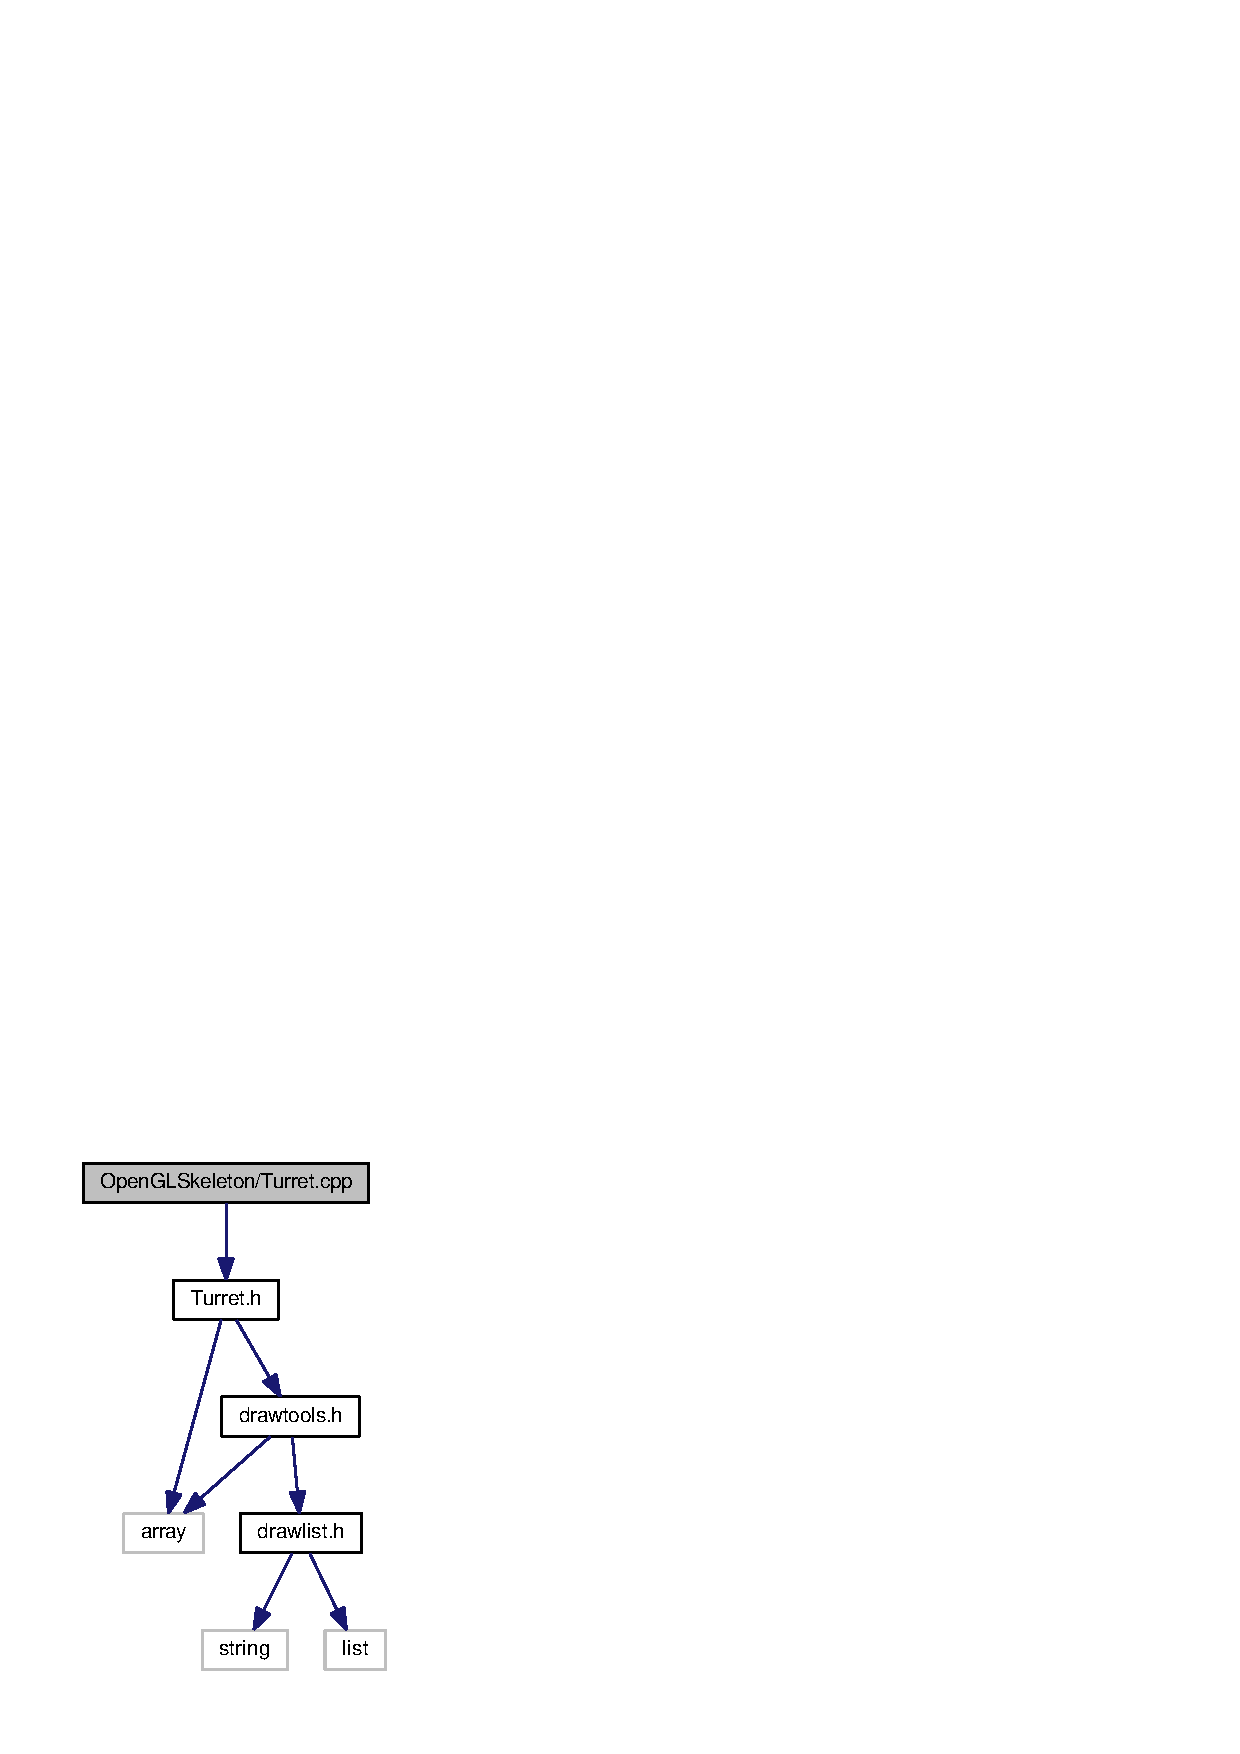
\includegraphics[width=225pt]{_turret_8cpp__incl}
\end{center}
\end{figure}

\hypertarget{_turret_8h}{}\section{Open\+G\+L\+Skeleton/\+Turret.h File Reference}
\label{_turret_8h}\index{Open\+G\+L\+Skeleton/\+Turret.\+h@{Open\+G\+L\+Skeleton/\+Turret.\+h}}
{\ttfamily \#include $<$array$>$}\\*
{\ttfamily \#include \char`\"{}drawtools.\+h\char`\"{}}\\*
Include dependency graph for Turret.\+h\+:
% FIG 0
This graph shows which files directly or indirectly include this file\+:
% FIG 1
\subsection*{Classes}
\begin{DoxyCompactItemize}
\item 
class \hyperlink{class_turret}{Turret}
\end{DoxyCompactItemize}

\hypertarget{zooi_8cpp}{}\section{Open\+G\+L\+Skeleton/zooi.cpp File Reference}
\label{zooi_8cpp}\index{Open\+G\+L\+Skeleton/zooi.\+cpp@{Open\+G\+L\+Skeleton/zooi.\+cpp}}

%--- End generated contents ---

% Index
\backmatter
\newpage
\phantomsection
\clearemptydoublepage
\addcontentsline{toc}{chapter}{Index}
\printindex

\end{document}
